%%%%%%%%%%%%%%%%%%%%%%%%%%%%%%%%%%%%%%
% yale_thesis.tex
% Alexander Cerjan
% 2014/04/07
%
% A bare, sample template for a Yale PhD thesis using yalephd.cls
%%%%%%%%%%%%%%%%%%%%%%%%%%%%%%%%%%%%%%

\documentclass[letterpaper,10pt]{yalephd}
% remove draft option for final printing.
% font size must be between 10pt-12pt.


\usepackage{soul}
\usepackage{enumitem}
\usepackage{bm}
\usepackage{amsmath}
\usepackage{gensymb}
\usepackage{subfigure}
\usepackage{multirow}
\usepackage{array}
\newcolumntype{L}{>{\centering\arraybackslash}m{2.5cm}}
\newcolumntype{K}{>{\centering\arraybackslash}m{2.2cm}}
\usepackage{hhline}
%\usepackage{minted}
\usepackage{listings}
\PassOptionsToPackage{hyphens}{url}
\usepackage{longtable}
\usepackage[font=small,labelfont=bf]{caption}

\usepackage{booktabs}

\usepackage{xcolor} % to access the named colour LightGray
\definecolor{LightGray}{gray}{0.95}

\usepackage{geometry} % you need this for yalephd.cls to work.
\usepackage{graphicx} % you probably want the rest of these.
\graphicspath{{./}{hsc_morph/images/}{gamornet/images/}{gampen/images/}{morph_den/images/}{intro_and_conc/images/}}
\usepackage{dcolumn}
\usepackage{bm}
\usepackage{amsfonts}
\usepackage{wrapfig}
\usepackage{amssymb}
\usepackage{appendix}
\usepackage{comment}
\usepackage{cite}
\usepackage{notoccite}
\usepackage{sectsty}
\usepackage[flushleft]{threeparttable}
\usepackage{pdflscape}
\usepackage{color}
\usepackage{hyperref}
\hypersetup{colorlinks=true, linkcolor = black, citecolor = blue}
\usepackage{xcolor}
\chapterfont{\Large\bfseries}
\sectionfont{\large\bfseries}
\usepackage{natbib}
\usepackage{bibentry}
\usepackage{commands}
\usepackage{rotating}
\usepackage[most]{tcolorbox}
\usepackage{tikz}

\makeatletter
\newcommand{\DrawLine}{%
  \begin{tikzpicture}
  \path[use as bounding box] (0,0) -- (\linewidth,0);
  \draw[color=blue!75!black,dashed,dash phase=2pt]
        (0-\kvtcb@leftlower-\kvtcb@boxsep,0)--
        (\linewidth+\kvtcb@rightlower+\kvtcb@boxsep,0);
  \end{tikzpicture}%
  }
\makeatother



\definecolor{codegreen}{rgb}{0,0.6,0}
\definecolor{codegray}{rgb}{0.5,0.5,0.5}
\definecolor{codepurple}{rgb}{0.58,0,0.82}
\definecolor{backcolour}{rgb}{0.95,0.95,0.92}

\lstdefinestyle{mystyle}{
    backgroundcolor=\color{backcolour},   
    commentstyle=\color{codegreen},
    keywordstyle=\color{magenta},
    numberstyle=\tiny\color{codegray},
    stringstyle=\color{codepurple},
    basicstyle=\ttfamily\footnotesize,
    breakatwhitespace=false,         
    breaklines=true,                 
    captionpos=b,                    
    keepspaces=true,                 
    numbers=left,                    
    numbersep=5pt,                  
    showspaces=false,                
    showstringspaces=false,
    showtabs=false,                  
    tabsize=2
}

\lstset{style=mystyle}


\usepackage{fontspec}
\newfontface{\bn}{kalpurush.ttf}


\newcommand\sersic{S\'ersic}
\newcommand\msun{$M_{\odot}$}
\newcommand\gamornet{G\textsc{a}M\textsc{or}N\textsc{et}}
\newcommand\gampen{GaMPEN}
\newcommand\lenstronomy{LENSTRONOMY}
\newcommand\grizy{\textit{grizy}}
\newcommand\uband{\textit{u}}
\newcommand\gb{\textit{g}}
\newcommand\rb{\textit{r}}
\newcommand\ib{\textit{i}}
\newcommand\zb{\textit{z}}
\newcommand\yb{\textit{y}}
\newcommand\om{\sim \mathcal{O}}


\begin{document}

% Need to define title before the abstract.
\title{Investigating Galaxy Morphology in Large Surveys Using Novel Machine Learning Frameworks} % capitalize the first letter in every word except conjunctions and prepositions
\author{\textbf{Aritra Ghosh} | \bn{অরিত্র ঘোষ}}
\advisor{Prof. C. M. Urry}
\date{December, 2023} % usually not \today.

% All the stuff at the front of your thesis.
\frontmatter

\begin{abstract}
asdjnfjins adsnfij snadijfn in iasndfinsjidnf ijjsndifjnsijdnf isjnadfn aoisjdfn iojansijdn
\end{abstract}


\maketitle
\makecopyright{2023} % change as needed.
\tableofcontents
\listoffigures % remove this if you have no figures.
\listoftables % remove this if you have no tables.

\chapter{Acknowledgements} % this needs to be before \mainmatter.


% Starts proper arabic numbering of pages and chapters.
\mainmatter

\chapter{Introduction} \label{chap:intro}

This is the introooooooo.
\chapter{Galaxy Morphology Network: A Convolutional Neural Network Used to Study Morphology and Quenching in $\sim 100,000$ SDSS and $\sim 20,000$ CANDELS Galaxies}

Originally published by the American Astronomical Society in \textit{The Astrophysical Journal}, Volume 895, Issue 2, pp. 112, DOI:\href{https://iopscience.iop.org/article/10.3847/1538-4357/ab8a47/meta}{10.3847/1538-4357/ab8a47}\\
{\large \emph{Aritra Ghosh, C. Megan Urry, Zhengdong Wang, Kevin Schawinski, Dennis Turp, and Meredith C. Powell} }\\


We examine morphology-separated color-mass diagrams to study the quenching of star formation in $\sim 100,000$ ($z\sim0$) Sloan Digital Sky Survey (SDSS) and $\sim 20,000$ ($z\sim1$) Cosmic Assembly Near-Infrared Deep Extragalactic Legacy Survey (CANDELS) galaxies. To classify galaxies morphologically, we developed Galaxy Morphology Network (\gamornet{}), a convolutional neural network that classifies galaxies according to their bulge-to-total light ratio. \gamornet{} does not need a large training set of real data and can be applied to data sets with a range of signal-to-noise ratios and spatial resolutions. \gamornet{}'s source code as well as the trained models are made public as part of this work (\href{http://www.astro.yale.edu/aghosh/gamornet.html}{Link\,1}$\vert$\href{http://gamornet.ghosharitra.com}{Link\,2}). We first trained \gamornet{} on simulations of galaxies with a bulge and a disk component and then transfer learned using $\sim25\%$ of each data set to achieve misclassification rates of $\lesssim5\%$. The misclassified sample of galaxies is dominated by small galaxies with low signal-to-noise ratios. Using the \gamornet{} classifications, we find that bulge- and disk-dominated galaxies have distinct color-mass diagrams, in agreement with previous studies. For both SDSS and CANDELS galaxies, disk-dominated galaxies peak in the blue cloud, across a broad range of masses, consistent with the slow exhaustion of star-forming gas with no rapid quenching. A small population of red disks is found at high mass ($\sim14$\% of disks at $z\sim0$ and 2\% of disks at $z \sim 1$). In contrast, bulge-dominated galaxies are mostly red, with much smaller numbers down toward the blue cloud, suggesting rapid quenching and fast evolution across the green valley. This inferred difference in quenching mechanism is in agreement with previous studies that used other morphology classification techniques on much smaller samples at $z\sim0$ and $z\sim1$.

\section{Introduction} \label{sec:intro}

We know from large-scale surveys that both local and high-redshift galaxies show a bimodal distribution in the galaxy color-mass space\,\citep{strateva_01,baldry_04,baldry_06,brammer_09} with a ``blue cloud,'' a ``red sequence'' and a ``green valley.'' Galaxy color-mass diagrams are useful for studying galactic evolution, as the stellar mass of a galaxy indicates its growth over time, and the color tracks its rate of star formation. The standard interpretation of the bimodal color-mass distribution is that, because there are few galaxies in the green valley, star formation in blue cloud galaxies must be quenched rapidly, perhaps aided by emission from an active galactic nucleus (AGN; \citealp{bell_04,faber_07}). Direct evidence of this AGN feedback remains murky, however \citep{harrison_17}.

Galaxy morphology adds a third interesting dimension to the color-mass space. Because elliptical galaxies typically form in major mergers, and galactic disks usually do not survive them, morphology can be used as a tracer of the recent merger history of a galaxy. The observed bimodality in the color-mass diagram (as well as interpretations therefrom) comes from superposing distinct populations with different morphological types, as first shown by \citet{schawinski_14_green_herring}, who used Galaxy Zoo morphological classifications to study local ($z\sim0$) galaxies. They suggested that there are two separate evolutionary tracks for galaxies: (1) major mergers forming ellipticals from disk-dominated galaxies, accompanied by AGN triggering and rapid quenching of star formation, and (2) slow, secular growth of disk-dominated galaxies, until they reach a critical halo mass, after which the remaining cold gas is slowly consumed and the stellar population gradually reddens. At $z\sim0$, the latter population is an order of magnitude larger than the merger-created ellipticals. 


\begin{figure*}[htbp]
	\begin{center}
	\begin{tabular}{cccc}
	\hline 
	\hline
	Disk-Dominated & Bulge-Dominated & Indeterminate & \\[0.15cm]
	\hline \\
    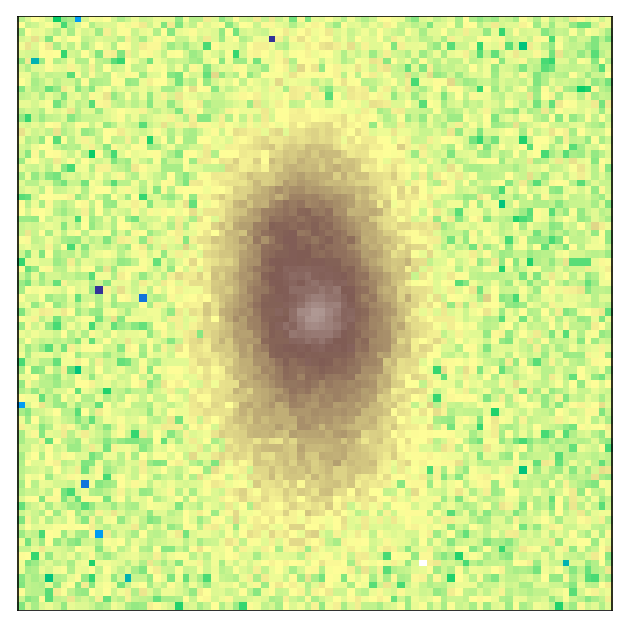
\includegraphics[width=3.25cm,height=3.25cm]{587722981750014081.pdf} & 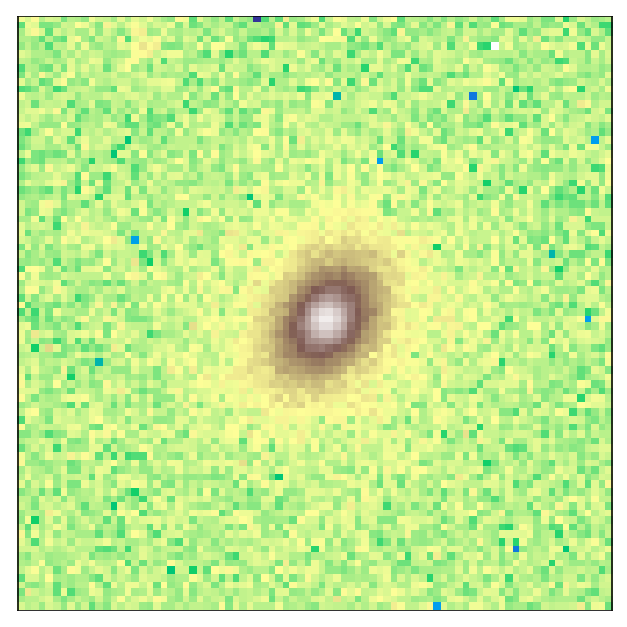
\includegraphics[width=3.25cm,height=3.25cm]{587724197741854834.pdf} & 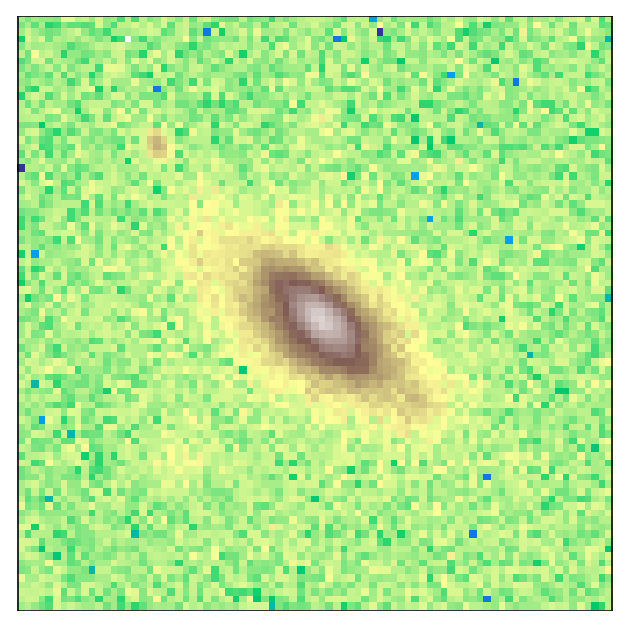
\includegraphics[width=3.25cm,height=3.25cm]{587722984443216081.pdf} &
     \multirow{2}{*}[2.5cm]{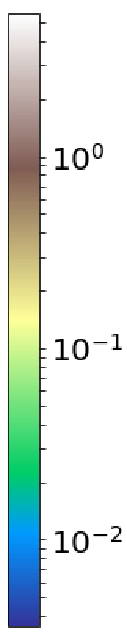
\includegraphics[height=6cm]{sdss_cbar.pdf}}
    \\[0.3cm]
     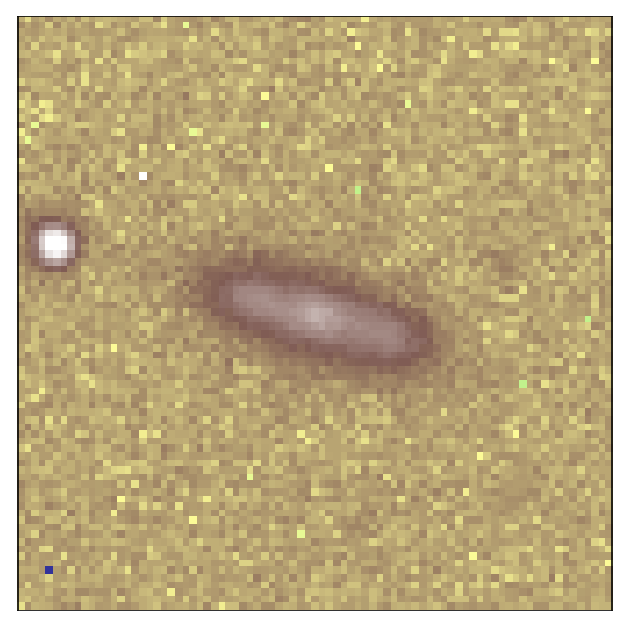
\includegraphics[width=3.25cm,height=3.25cm]{587722983369408606.pdf} & 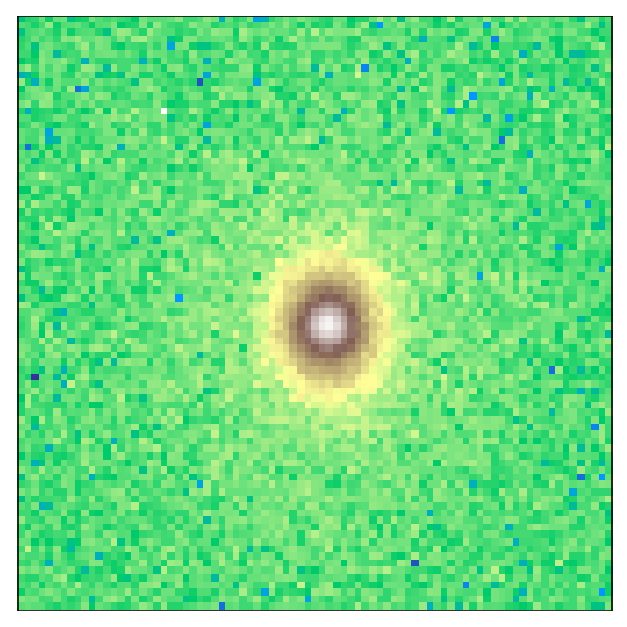
\includegraphics[width=3.25cm,height=3.25cm]{587724198278725806.pdf} & 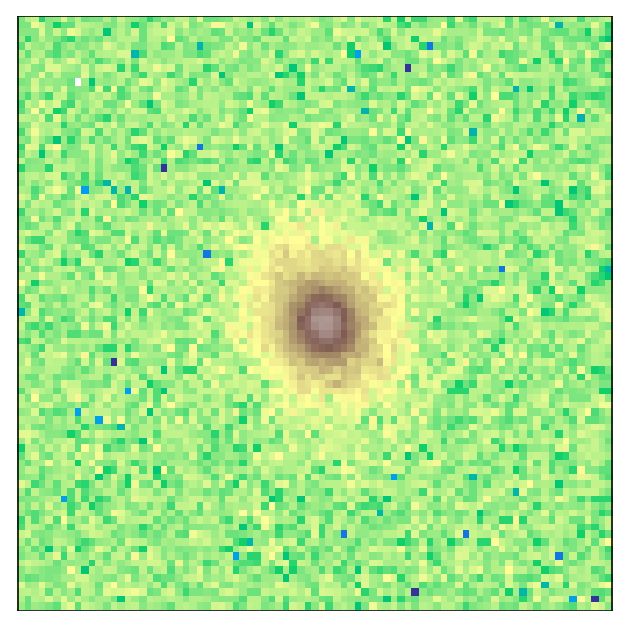
\includegraphics[width=3.25cm,height=3.25cm]{587724232641937529.pdf}
     &
     \\[0.3cm]
     \hline
     \\
      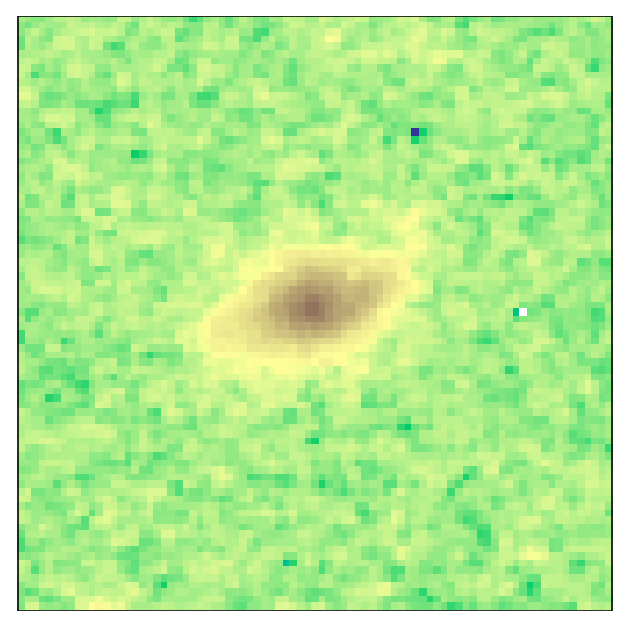
\includegraphics[width=3.25cm,height=3.25cm]{goodsn_93.pdf} & 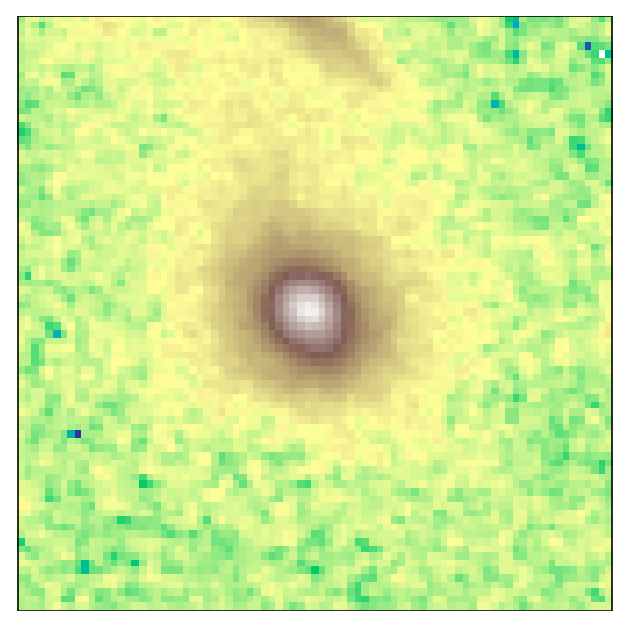
\includegraphics[width=3.25cm,height=3.25cm]{goodsn_750.pdf} & 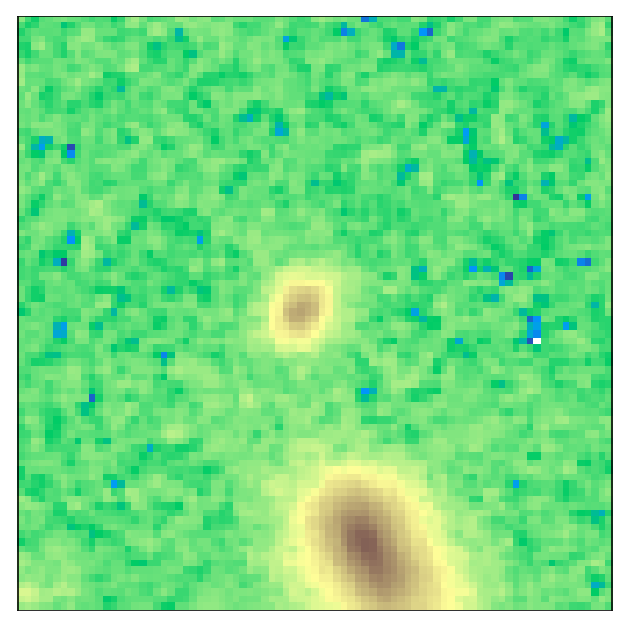
\includegraphics[width=3.25cm,height=3.25cm]{goodsn_88.pdf} &
     \multirow{2}{*}[2.5cm]{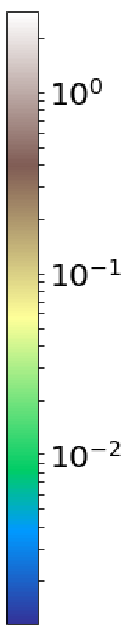
\includegraphics[height=6cm]{candels_cbar.pdf}}
     \\[0.3cm]
     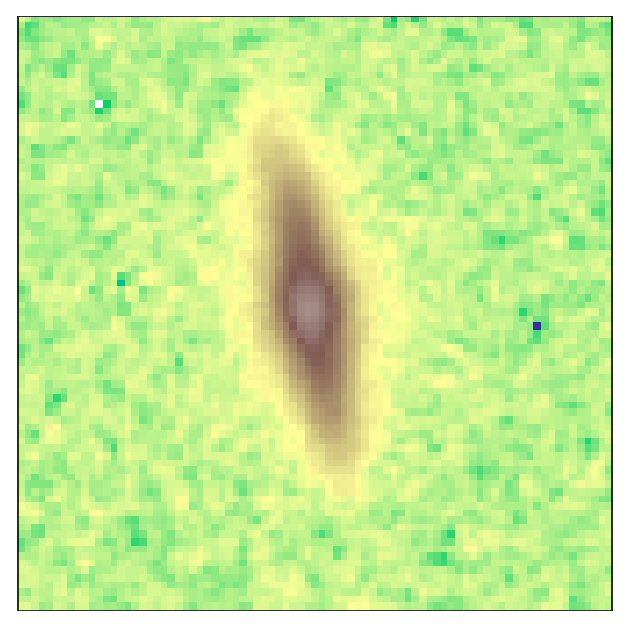
\includegraphics[width=3.25cm,height=3.25cm]{goodss_6472.pdf} & 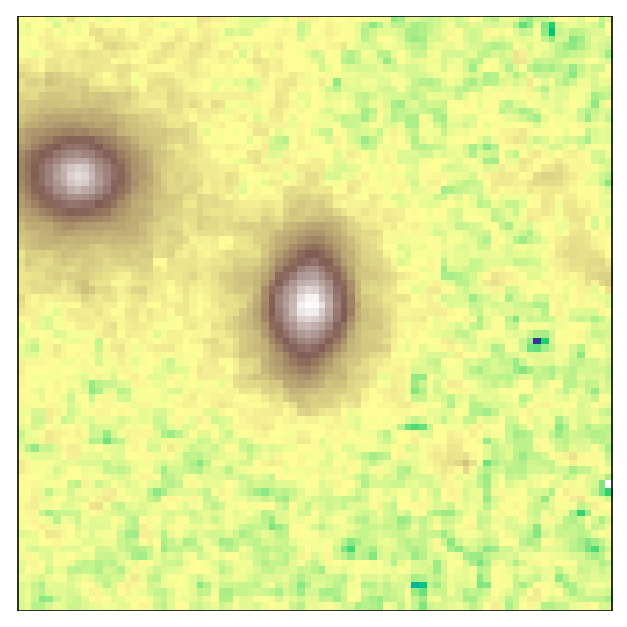
\includegraphics[width=3.25cm,height=3.25cm]{goodsn_1029.pdf} & 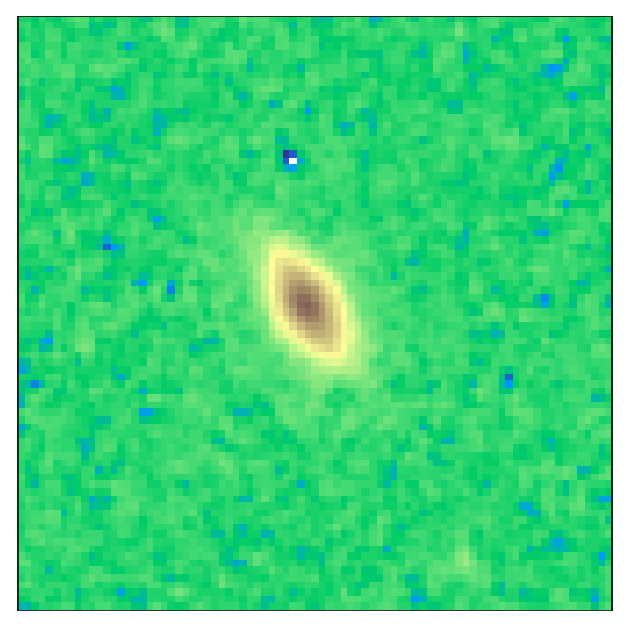
\includegraphics[width=3.25cm,height=3.25cm]{goodss_11555.pdf} 
     & 
     \\[0.3cm]
     \hline
    \end{tabular}
  \end{center}
  \caption{The above figure contains randomly chosen galaxies from both our data sets classified by \gamornet{} as being disk-dominated\,(left column panels), bulge-dominated\,(middle column panels) or indeterminate\,(right column panels). Refer to \S~\ref{sec:morph_results} for the definitions of these categories. The top two rows show SDSS cutouts, which are 33.07" $\times$ 33.07" (83 pixels $\times$ 83 pixels) and the bottom two rows show CANDELS cutouts, which are 4.98" $\times 4.98"$ (83 pixels $\times$ 83 pixels). During training, \gamornet{} focuses on galaxies located at the center of the image and, thus, can process cutouts with other objects in the frame besides the central galaxy, as is evident from the images above.}
  \label{fig:eg_images}
\end{figure*}


Still, most star formation and the most pronounced galaxy evolution happen not locally but at $z\sim1$ and above. Thus, it is important to investigate the galaxy color-mass diagram at $z\gtrsim1$. \citet{powell_17} studied galaxies from The Great Observatories Origins Deep Survey\,(GOODS)-N and GOODS-S at $z\sim1$ and found that disks and spheroids have distinct color-mass distributions in rough agreement with the results at $z\sim0$. From the distribution of X-ray-selected AGN hosts in this sample, they concluded that AGN feedback may quench star formation in galaxies that undergo major mergers, but these are still less than half the galaxy population. However, this study was done with a sample of only $2651$ disks and $126$ spheroids. Much larger studies, across a broader redshift range, will better illuminate the effect of mergers and AGN on galaxy evolution. 

The two traditional ways of obtaining morphological classifications --- visual classification and fitting light profiles --- are not easily scalable to the large data volumes expected from The Large Synoptic Survey Telescope\,(LSST), the Wide Field Infrared Survey Telescope\,(WFIRST) and Euclid. The most popular galaxy light profile fitting program, GALFIT\,\citep{galfit}, and automated versions of it like GALAPAGOS\,\citep{galapagos}, suffer from the fact that the quality of the fit depends heavily on the input parameters, and when dealing with hundreds of thousands of galaxies, such hand-refinement of input parameters is an impossible task. There have been attempts to employ visual classifications on large galaxy samples via citizen science projects like Galaxy Zoo\,\citep{gzoo_p1,gzoo_p2}, but even these will fail to keep up with the coming data volume. Moreover, reliable visual classifications require a decent signal-to-noise ratio (S/N), take time to set up and execute, and require an extremely careful de-biasing of the vote shares obtained \citep{gzoo_p1,gzoo_candels}. 

For these reasons, using machine learning to classify galaxy morphology is particularly attractive. Data available from the Sloan Digital Sky Survey\,(SDSS) inspired early attempts at using machine learning to classify galaxies morphologically on a large scale\,\citep[e.g.,][]{Ball2004GalaxyNetworks,Kelly2004MorphologicalSurvey,banerji_10}. These methods required the user to select proxies for morphology (such as color, concentration index, and spectral features) as inputs to the models. However, as the proxies could have an unknown and biased relation with galaxy morphology, these early networks were not ideal substitutes for the traditional classification methods. 

In the last few years, convolutional neural networks\,(CNNs) have revolutionized the field of image processing\,\citep{dl_1,dl_2}. They are ideal for galaxy morphology classification as they do not require selection of morphological proxies by hand and the network itself decides on which features of the image best discriminate among the different classes. The first serious attempt at using a CNN to classify galaxies morphologically came out of the ``Galaxy Challenge" organized by Galaxy Zoo, where teams competed to reproduce the vote shares of each question in Galaxy Zoo 2 using a CNN (the top entry was by \citealp{dieleman_15}). This was followed by the work of \citet{company_15}, who used a CNN to reproduce visual classifications for galaxies in the Cosmic Assembly Near-Infrared Deep Extragalactic Legacy Survey\,(CANDELS). \citet{tuccillo_18} used domain adaptation combined with one-component Se\'rsic simulations to reproduce morphological classifications for $\sim 5000$ CANDELS galaxies. There have also been attempts at using CNNs for measuring photometric redshifts from galaxy images\,\citep{ml_pz}, doing star/galaxy separation\,\citep{ml_sz}, detecting bars in galaxies\,\citep{ml_bars} and detecting mergers\,\citep{ml_mergers}. 

Most of the previous work involving the use of CNNs to study galaxy morphology has depended on the availability of a large training set of galaxies with known properties. However, if CNNs are to truly replace traditional methods for morphology classification, then there needs to be a single prescription/network that works across multiple data sets and does not require an already classified large training set. 

In this paper, we introduce Galaxy Morphology Network (\gamornet{}), a CNN that can classify galaxies according to their bulge-to-total ratio ($L_B/L_T$) for very different data sets without the need for a large,  pre-classified training set of real galaxies. We first trained our network on simulated galaxies with both bulge and disk components and then transfer learned on a small part of our real sample to produce bulge/disk classifications for $\sim80,000$ ($z \sim 0$) SDSS \textit{g}-band galaxies and $\sim20,000$ CANDELS ($z \sim 1$) \textit{H}-band galaxies. A collection of 12 randomly chosen galaxy image cutouts from both data sets with their \gamornet{} classifications is shown in Figure~\ref{fig:eg_images}. Using the morphology classifications, we then examine the color-mass diagrams of the two samples, separated by morphology, in order to study the quenching of star formation at $z\sim0$ and $1$. 

We describe the details of the SDSS and CANDELS data that we use in \S~\ref{sec:data}. In \S~\ref{sec:methods}, we describe our simulations, the CNNs we use, and our transfer learning algorithm. In \S~\ref{sec:results}, we present the results of the morphology classification, including the color-mass diagrams, and in \S~\ref{sec:disc}, we summarize our results and discuss future applications of \gamornet{}.

We make all of the source code used in this work public along with the trained CNN models. We also release the \gamornet{} morphological predictions for all of the SDSS and CANDELS galaxies in our data sets. All of the code is being made available under a GNU General Public License v3.0 and more details of the public data release are summarized in Appendix\,\ref{sec:ap:public_data_release}. 

\section{Data Sets Used} \label{sec:data}

One of the primary aims of this paper is to demonstrate how \gamornet{} can be used to identify bulge- and disk-dominated galaxies in different data sets without requiring extensive training on real data. Here, we work with two data sets: the SDSS \citep{sdss_tech_summary}, for nearby galaxies ($z\sim0$), and CANDELS \citep{candels_1,candels_2}, for galaxies at $z\sim1$. Together, these data allow us to probe galaxy evolution at different epochs of star formation and black hole growth.

We first created galaxy samples with which we train and test \gamornet{}. Specifically, we identified galaxies in each survey for which bulge/disk decomposition had already been done or which had already been morphologically classified in some other way. 

For the SDSS sample, we used $112,547$ galaxies in the redshift range $ 0.02 \leq z \leq 0.07$ that were imaged in the $g$ band and had bulge fractions determined by \citet{simard_11}, who fitted double \sersic{} profiles with fixed indices $n = 4$ (pure bulge) and $n=1$ (pure disk). For each galaxy, we prepared square cutouts of 167 pixels on a side, centered on the galaxy, with a resolution of $0.396''$ per pixel. We used 30,000 of these for the process of transfer learning, described in \S\,\ref{sec:tf_intro} and the remaining 82,547 galaxies to test the performance of the network. In order to calculate the \textit{u-r} color for each galaxy, we used extinction-corrected model SDSS magnitudes from the NYU-VAGC\,\citep{nyu_vagc_des} and adopted K corrections to $z=0.0$. We obtained aperture and extinction-corrected specific star formation rates (sSFR) and stellar masses from the MPA-JHU DR7 catalog\,\citep{mpa_jhu_2,mpa_jhu_1}, which are calculated using SDSS spectra and broadband photometry. 

For CANDELS reference data, we used \sersic{} indices from \citet{vdw_12}, who fitted the galaxy surface brightness profiles using GALFIT \citep{galfit} with a single (free) \sersic{} component. From this catalog, we selected galaxies with redshifts $0.7 \leq z \leq 1.3$ and ``good" fits (defined by \citealp{vdw_12} as matching the galaxy total magnitude, and having fits that converged, with parameters within an acceptable range). The ensuing sample of 28,946 $z\sim1$ galaxies from the five CANDELS fields includes 6276 from the Great Observatories Origins Deep Survey--North (GOODS-N), 3942 from the Great Observatories Origins Deep Survey--South (GOODS-S), 7425 from the Cosmic Evolution Survey (COSMOS), 4911 from the Ultra Deep Survey (UDS) and 6392 from the All Wavelength Extended Growth Strip International Survey (AEGIS). We downloaded WFC3/IR F160W(H) mosaics from the CANDELS website\footnote{\href{http://arcoiris.ucolick.org/candels/data\textunderscore access/Latest\textunderscore Release.html}{http://arcoiris.ucolick.org/candels/data\textunderscore access/Latest\textunderscore Release.html}}, then for each galaxy, we made square cutouts of $83$\,pixels$\times83$\,pixels with a resolution of $0.06''$ per pixel. We used 7200 galaxy images for transfer learning and the remaining 21,746 for testing the performance of \gamornet{}. We took the rest-frame \textit{U-R} color, stellar mass, and sSFR of each galaxy from the 3D-HST catalog \citep{3dhst}; the stellar masses are based on spectral energy distribution\,(SED) fits to stellar population models with the FAST code \citep{fast} as described in \citet{skelton_14}. The star formation rates used are from \cite{whitaker_14} and assume that UV light from massive stars is re-radiated in the far-infrared.


\begin{table*}[htbp]
\centering
\caption{Parameter Ranges for Simulated Galaxies  \label{tab:sim_para}}
\begin{tabular}{cccccc}
\hline
\hline
Component& \sersic{} & Radius & Magnitude & Axis Ratio & Position Angle \\ 
Name & Index & (Pixels) & (AB) &  & (degrees) \\
\hline
\hline
\multicolumn{6}{c}{SDSS sample at $z \sim 0$} \\
    \hline
    Disk & 1.0 & 10.0 - 30.0 & 15.0 - 22.0 & 0.3 - 1.0 & -90.0 - 90.0 \\
    %\hline
    Bulge & 4.0 & 4.0 - 17.0 & Disk $\pm\,(0,3.2)^{a}$ & 0.3 - 1.0 & Disk $\pm\,(0,15)^{b}$\\
    \hline
    \hline
    \multicolumn{6}{c}{CANDELS sample at $z \sim 1$} \\
    \hline
    Disk & 1.0 & 12.0 - 25.0 & 17.0 - 27.8 & 0.3 - 1.0 & -90.0 - 90.0\\
    %\hline
    Bulge & 4.0 & 4.0 - 14.0 & Disk $\pm\,(0,3.2)^{a}$ & 0.3 - 1.0 &  Disk $\pm\,(0,15)^{b}$ \\
    \hline
    \multicolumn{6}{p{0.9\textwidth}}{\vskip 0.01cm \small $^a$The bulge magnitude differs from the disk magnitude by a randomly chosen value between $-3.2$ and $+3.2$}\\
    \multicolumn{6}{p{0.9\textwidth}}{\small$^b$The bulge position angle differs from the disk position angle by a randomly chosen value between $-15$ and $+15$}\\
    \multicolumn{6}{p{0.9\textwidth}}{\small \texttt{NOTE-} The above table shows the ranges of the various \sersic{} profile parameters used to simulate the training data. Each simulated galaxy has an $n=1$ disk and an $n = 4 $ bulge component, where n is the \sersic{} index. The distributions of all the simulated parameters are uniform except those for the bulge magnitude and bulge position angle. See \S\,\ref{sec:simulation_code} for more details.}\\
\end{tabular}
\end{table*}


It is well known that dust extinction can redden galaxies, and significant reddening has been observed for high-redshift galaxies\,\citep{brammer_09,williams_09,cardamone_10}. For the SDSS sample, we make no reddening correction since \citet{schawinski_14_green_herring} showed that dust correction has a negligible effect on the color-mass diagram for local galaxies. However, for the higher redshift CANDELS sample, we corrected the \textit{U-R} colors using the \citet{calzetti_00} extinction law:

\begin{equation}
    \Delta (U-R) = 0.65 A_V  .
\end{equation}

\noindent
The $A_V$ values, taken from the 3D-HST catalog, come from SED fits to stellar population models \citep{3dhst}. 

For both data sets, we used only a fraction of the available sample for transfer learning, leaving a much larger fraction for testing the performance of \gamornet{}. This demonstrates that \gamornet{} can effectively be trained initially on (more extensive) simulations, then re-trained using a small set of real data. Thereafter, \gamornet{} can successfully classify a much larger set of real images because it learns to generalize beyond the training galaxies.


\section{Training our Convolutional Neural Network --- \gamornet{}} \label{sec:methods}

The first hurdle in training a neural network to do morphological classifications is finding a large data set that has already been accurately classified. However, if neural networks are to be used widely for astronomical analysis, we need a more flexible approach --- one that does not require extensive analysis by old, slow (legacy) methods during the training phase and that can be adapted easily to new data sets. Here, we describe how to use simulated galaxies for the initial training of the classification network, followed by the application of a machine learning technique known as ``transfer learning'', wherein a much smaller set of galaxies, classified using a legacy method, is used to fine tune a partially trained network. This ensures that the network becomes adept at classifying real galaxies without requiring too many of them for the training process.

The process of training \gamornet{} to classify galaxy morphologies consists of the following steps:
\begin{enumerate}[noitemsep]
\item Simulating galaxies corresponding to the desired data set (here, SDSS or CANDELS).
\item Initial training of the neural network on those simulated images.
\item Retraining the neural network using a small part of the real data at hand; this process is known as transfer learning.
\item Testing a similar amount of real data to validate the results.
\item Processing the remainder of the real data through the trained network to obtain morphological classifications. 
\end{enumerate}
 
The galaxy simulations are described in \S\,\ref{sec:simulation_code}. \S\,\ref{sec:network_description} contains a brief introduction to CNNs and describes the architecture of \gamornet{}, while \S\,\ref{sec:initial_training} describes the initial training of \gamornet{} on the simulations. In \S\,\ref{sec:tf_intro}, we describe how we perform transfer learning to produce the final trained state of \gamornet{}.

\subsection{Simulations} \label{sec:simulation_code}

\begin{figure*}[hbt]
	\begin{center}
    \subfigure[Initial Simulated Image]{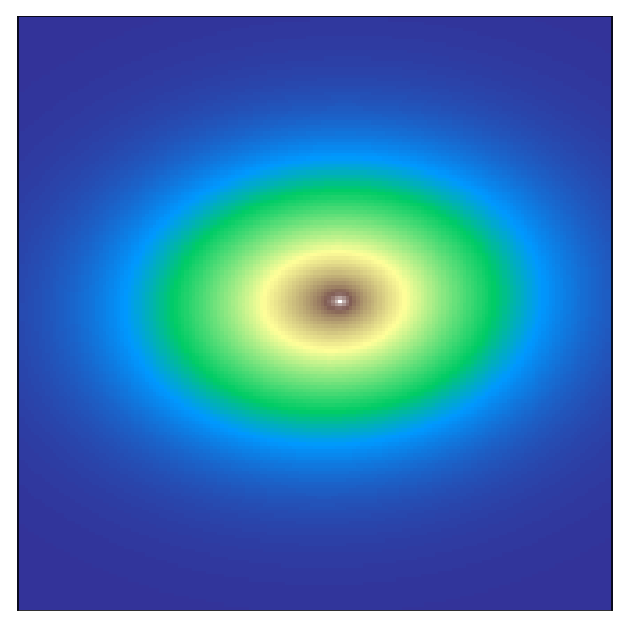
\includegraphics[width=4cm,height=4cm]{output_img_88728.pdf}} 
    \subfigure[Convolved with PSF]{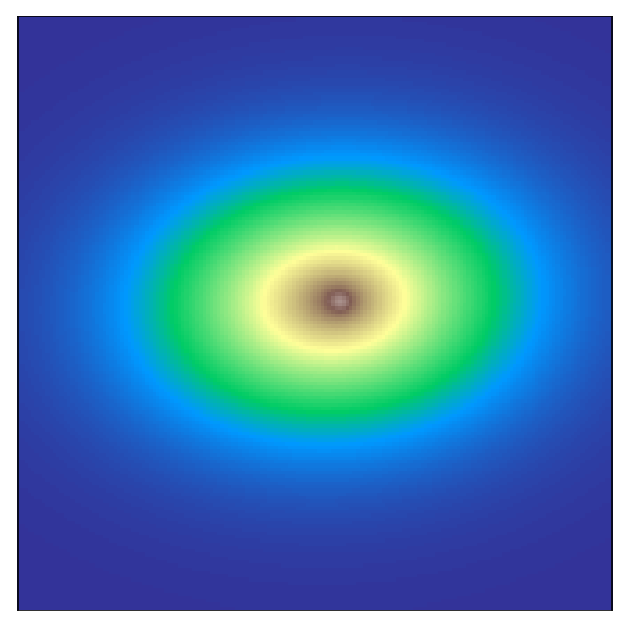
\includegraphics[width=4cm,height=4cm]{convolved_img_88728.pdf}} 
    \subfigure[Noise Added]{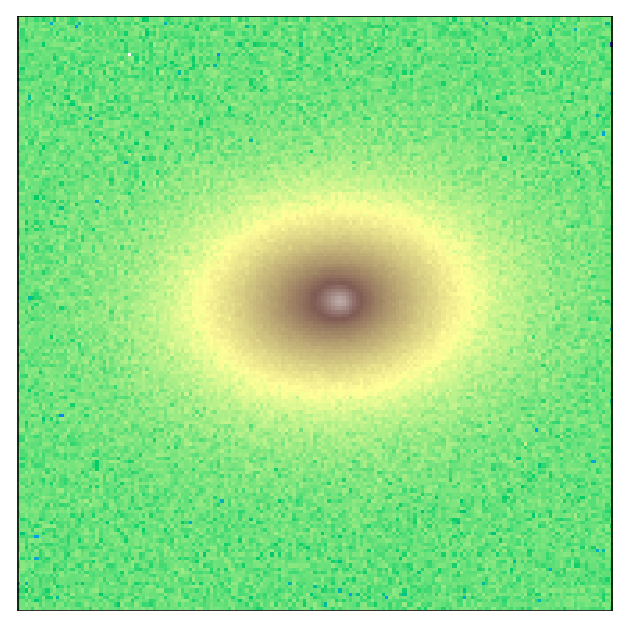
\includegraphics[width=4cm,height=4cm]{final_img_88728.pdf}} 
     \subfigure{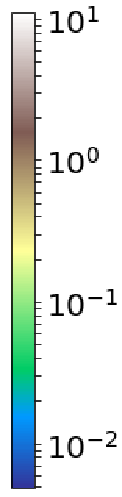
\includegraphics[height=4cm]{cbar_sim_noise.pdf}} 
  \end{center}
  \caption{Three stages in simulating an SDSS galaxy. Left (a): Light profile generated by GALFIT with a bulge-to-disk ratio of 0.24. Center (b): The left image convolved with the SDSS PSF. Right (c): SDSS noise added to the middle image. See \S\,\ref{sec:simulation_code} for details of the PSF convolution and noise addition.}
  \label{fig:psf_noise}
\end{figure*}

We simulated galaxies using the GALFIT program \citep{galfit}, which is usually used to fit two-dimensional light profiles of galaxies. Here, we use it instead to create two-dimensional light profiles appropriate for the data sets we are interested in analyzing with \gamornet{}.

For each data set, we simulated 100,000 galaxies consisting of a bulge (\sersic{} component with fixed index $n=4$;\,\citet{de_vac_48}) and disk (\sersic{} index $n=1$). The surface brightness for a galaxy with a \sersic{} profile is given by

\begin{equation}
\label{eq:sersic_fn}
\Sigma(r) = \Sigma_e \exp \left[ -\kappa \left( \left( \frac{r}{r_e}\right)^{1/n} - 1 \right) \right] ,
\end{equation}
where $\Sigma_e$ is the pixel surface brightness at the effective radius $r_e$, $n$ is the Se\'rsic index, which controls the concentration of the light profile, and $\kappa$ is a parameter coupled to $n$ that ensures that half of the total flux is enclosed within $r_e$.


The parameters required to generate the \sersic{} profiles are drawn from uniform distributions (except the bulge magnitude and position angle) and the ranges of the distributions used for both sets of simulations are summarized in Table~\ref{tab:sim_para}. The galaxy size parameters were chosen to be representative of bright, local galaxies \citep{binney_and_merrifield}; bulges were chosen to have a half-light radius between $3.0$\,kpc and $6.0$\,kpc and disks were assigned half-light radii between $6.0$\,kpc and $10.0$\,kpc. To obtain the corresponding pixel sizes, we placed the samples at $ z = 0.05$ and $z = 1.0$ (corresponding to the mean redshifts of the two samples described in \S\,\ref{sec:data}) using WMAP7 cosmology \citep{wmap7} and using the pixel scale for the appropriate data set. We ensured that the number of simulated galaxies was sufficiently large such that even when we consider subsets of galaxies with similar sizes, they not only span the entire range of $L_B/L_T$ values but also mimic the overall bulge-to-total light ratio distribution.  

The disk magnitudes were drawn from a uniform distribution chosen so as to include most galaxies at these redshifts, and the magnitude of each corresponding bulge is such that it differs from the disk magnitude by a randomly chosen value between $-3.2$ and $3.2$. This was done to ensure that the bulge-to-total ratio varies between $\sim 5\% - 95\%$. Not enforcing this condition and allowing the bulge magnitude to be independent of the disk magnitude causes most galaxies in the training set to have a very high or a very low bulge-to-total ratio, which is not the case for most galaxies and, in any case, is not detectable. Instead, we want to train the network on a sufficient number of galaxies with intermediate bulge-to-total ratios.  

To make the two-dimensional light profiles generated by GALFIT more closely resemble the actual data, we convolved them with a representative point-spread function (PSF), then added noise. For the SDSS simulations, we selected the coordinates of one of the real galaxies in our sample -- R.A.: $213.26064353$, Decl.: $0.14637573$ and then reconstructed the PSF at the corresponding location in the detector using the PSF information stored in the relevant psField file that we obtained from SDSS. To generate the representative noise, we randomly selected 1000 cutouts from our SDSS sample, masked the sources in each cutout using SourceExtractor \citep{s_extract} and then read-in the non-masked pixel values to generate a large sample of noise pixels. We sampled this collection of noise pixels randomly to make two-dimensional arrays of the same size as that of the simulated images and then added them to the images. To make sure that the PSF chosen is representative, we reconstructed the PSFs for 12 more randomly chosen galaxies in our sample and convolved each one with a simulated SDSS galaxy, before adding noise. By inspecting the difference images between each image created using one of the new PSFs and the image created using the originally used PSF, we found the average pixel value of each of these difference images to be at least three orders of magnitude lower than the average pixel value of the galaxy image created using the original PSF.


For the CANDELS sample, we used the model PSF generated by \citet{vdw_12} for the COSMOS field and added noise following the same method as for the SDSS simulations. To make sure that the COSMOS PSF is representative, we followed a procedure similar to what we did for SDSS using the GOODS-S and UDS PSFs. We again found the average pixel value of the difference images to be at least three orders of magnitude lower than the average pixel value of the galaxy image created using the original PSF. 

The effect of convolving the simulated galaxies with PSF and adding noise is depicted in Figure~\ref{fig:psf_noise}.

The goal behind convolving with the PSF and adding noise is not to recreate perfect replicas of the real galaxies in our samples but rather to train the network on realistic simulated images for which we know the intrinsic morphologies. This is why we arbitrarily selected the COSMOS PSF instead of making simulations for each field separately and used only one random SDSS PSF. If we were to make more of an effort to recreate exactly the real data in our sample, then the whole purpose having a CNN is lost. In that case, the neural network ends up having a low variance but an extremely high bias, as it is too closely tied to the training set. Instead, here, the CNN learns to generalize from fewer examples.  

Since the galaxies were independently simulated, the simulation code could be trivially parallelized, and we make the simulation code available as a part of our public data release (see Appendix \ref{sec:ap:galsim}).


\subsection{The Network} \label{sec:network_description}
Artificial neural networks, consisting of many connected units called artificial neurons, have been studied for more than five decades now. The neurons are arranged in multiple layers as shown in the schematic representation in Figure~\ref{fig:schematic_network}; each network has an input layer via which the data is fed into the network and an output layer that contains the result of propagating the data through the network, with additional hidden layer(s) in between. Each neuron is characterized by a weight vector $\bm{w}=(w_1,w_2,\ldots,w_n)$ and a bias $b$. The input to a neuron (coming from the outputs in the previous layer) is usually written as $\bm{x}=(x_1,x_2,\ldots,x_n)$ and the output of the neuron is given by 

\begin{equation}
y = \sigma(\bm{w} \cdot \bm{x} + b) ,
\label{eq:neuron_output}
\end{equation}
where $\sigma$ is the chosen activation function of the neuron. The process of ``training" an artificial neural network involves finding out the optimum set of weights and biases of all the neurons such that for a given vector of inputs, the output vector from the network, $\bm{y} = (y_1,y_2,\ldots,y_n)$, resembles the desired output vector $\bm{\hat{y}}=(\hat{y_1},\hat{y_2},\ldots,\hat{y_n})$ as closely as possible. The process of optimization is usually performed by minimizing a loss function, such as the popular cross-entropy loss function,

\begin{equation}
L = -\frac{1}{N}\sum_{j=1}^N \sum_{c=1}^M I_{j,c} \log(p_{j,c}) 
\label{eq:cross_entr_loss}
\end{equation}
where $I_{j,c}$ is a binary indicator function depicting whether class label $c$ is the correct classification for the $j^{th}$ observation. Also, $p$ is the predicted probability (by the network) that observation $j$ is from class $c$, $M$ is the total number of classes and $N$ is the total number of samples. 

\begin{figure}[htbp]
	\begin{center}
		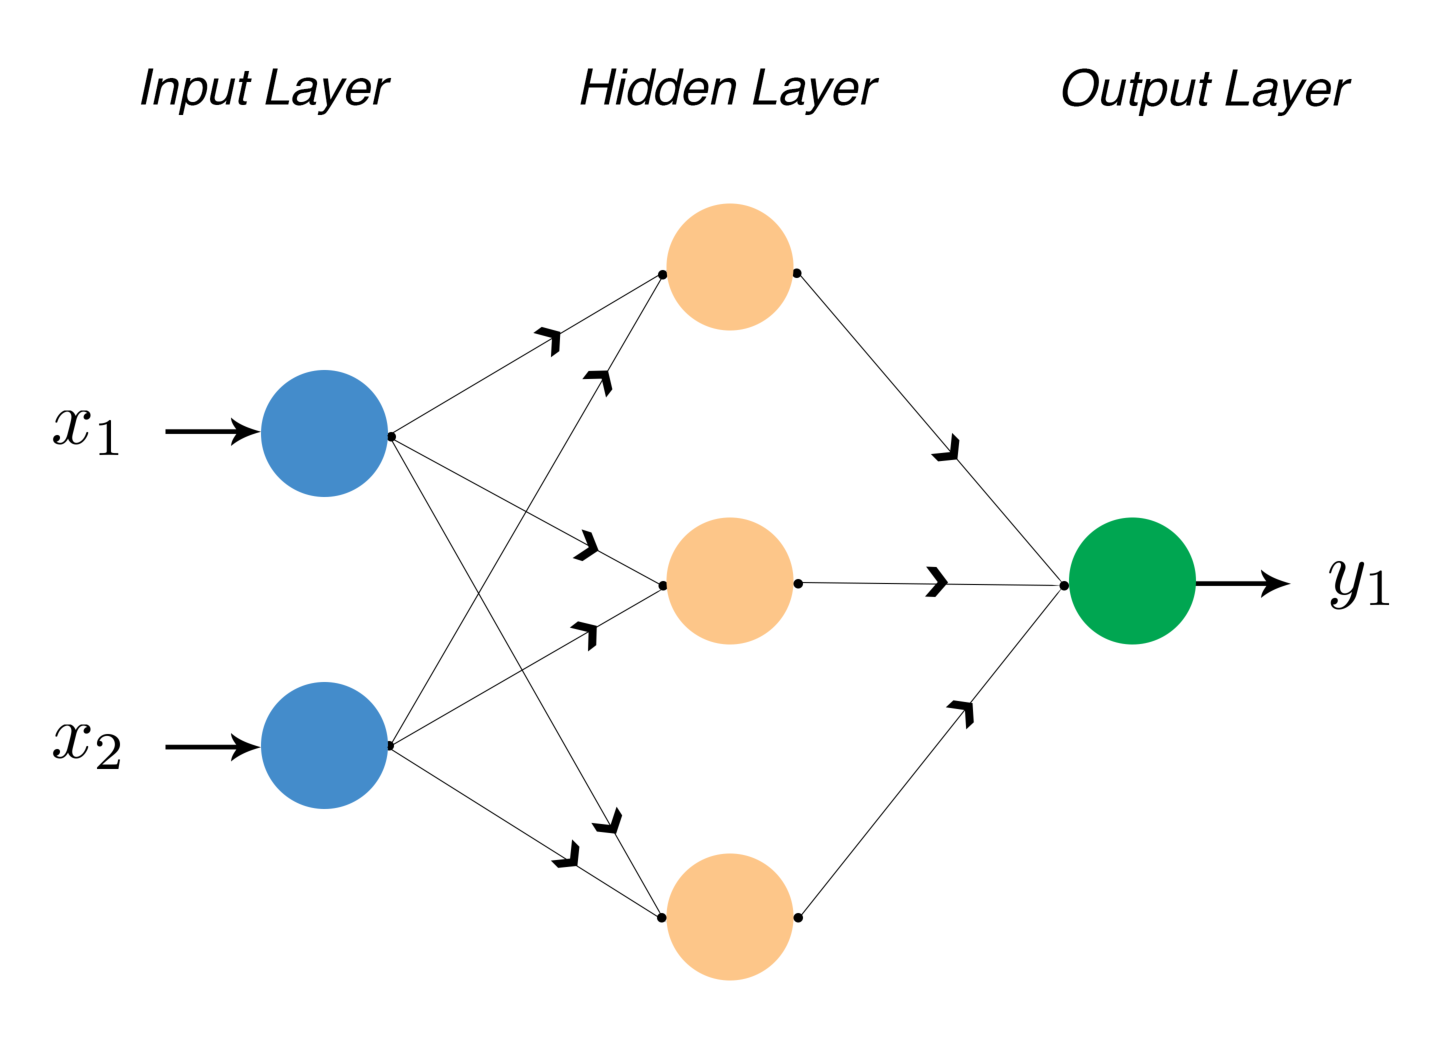
\includegraphics[width=0.6\textwidth]{schematic_toy_network.pdf}
	\end{center}
	\caption{A schematic diagram showing a simple artificial neural network with a single hidden layer.}
	\label{fig:schematic_network}
\end{figure}

Out of the various algorithms available to minimize the loss function, one that is used very widely is stochastic gradient descent\,(SGD) and its different variants \citep{nielsen}. In SGD, we estimate the gradient of $L$ using a mini-batch of training samples and update the weights and biases according to

\begin{equation}
\begin{aligned}
w' = w -\eta \frac{\partial L}{\partial w} \\
b' = b - \eta \frac{\partial L}{\partial b}
\end{aligned}
\label{eq:sgd}
\end{equation}
where $\eta$ is a small positive constant known as the learning rate. Calculation of the gradient is done using the back-propagation algorithm, and we refer the interested reader to \citet{rumelhart_88} for details.

\begin{table*}
  \centering
  \caption{Structure of \gamornet{} \label{tab:network_layers}}
  \begin{tabular}{cccc}
  \hline
  \hline
  Order & Type of Layer & Layer Description & Activation Function \\
  \hline
  1 & Input & $167\times167$(SDSS) $\vert$ $83\times83$(CANDELS) & --  \\
  \hline
  2 & Convolutional & Filters: 96 $\vert$ Filter Size: 11 $\vert$ Strides: 4 & ReLU\textsuperscript{a} \\
  \hline   
  3 & Max-Pooling & Kernel Size: 3 $\vert$ Strides: 2 & -- \\
  \hline
  4 & Loc. Response Norm. & -- & -- \\
  \hline
  5 & Convolutional & Filters: 256 $\vert$ Filter Size: 5 $\vert$ Strides: 1 & ReLU\textsuperscript{a} \\
  \hline   
  6 & Max-Pooling & Kernel Size: 3 $\vert$ Strides: 2 & -- \\
  \hline
  7 & Loc. Response Norm. & -- & -- \\
  \hline
  8 & Convolutional & Filters: 384 $\vert$ Filter Size: 3 $\vert$ Strides: 1 & ReLU\textsuperscript{a} \\
  \hline
  9 & Convolutional & Filters: 384 $\vert$ Filter Size: 3 $\vert$ Strides: 1 & ReLU\textsuperscript{a} \\
  \hline
  10 & Convolutional & Filters: 256 $\vert$ Filter Size: 3 $\vert$ Strides: 1 & ReLU\textsuperscript{a} \\
  \hline
  11 & Max-Pooling & Kernel Size: 3 $\vert$ Strides: 2 & -- \\
  \hline
  12 & Loc. Response Norm. & -- & -- \\
  \hline
  13 & Fully Connected & No. of neurons: 4096 & tanh \\
  \hline
  14 & Dropout & Dropout probability: 50$\%$ & -- \\
  \hline
  15 & Fully Connected & No. of neurons: 4096 & tanh \\
  \hline
  16 & Dropout & Dropout probability: 50$\%$ & -- \\
  \hline
  17 & Fully Connected & No. of neurons: 3 & softmax \\
  \hline
  \multicolumn{4}{p{0.93\textwidth}}{\vskip 0.1cm \small \textsuperscript{a}Rectified Linear Unit} \\
  \multicolumn{4}{p{0.93\textwidth}}{\small \texttt{NOTE-} The various layers of \gamornet{} along with the important parameters of each layer and the corresponding activation functions are shown in the table above. The architecture of \gamornet{} is based on AlexNet and, broadly speaking, consists of five convolutional layers followed by three fully connected layers. The source code for \gamornet{} is made public as described in Appendix\,\ref{sec:ap:gamornet_source_code}} \\
  \end{tabular}
\end{table*}

The artificial neural network that we use for this work is a Convolutional Neural Network (CNN; \citealp{fukushima_80, lecun_98}). This is a type of deep artificial neural network that has become extremely popular for image processing in recent years. The input to the network is the two-dimensional vector representation of an image, and in a convolutional layer, each unit receives input from a local image patch of the previous layer known as the receptive field. Convolution involves taking a filter of a particular size and repeatedly applying it (by moving it with a specific stride) to each part of the input image, resulting in a two-dimensional output map of activations called a feature map. The different units in the feature map share the same weight matrix, and hence, each feature map can be interpreted as trying to locate a particular feature at different locations in the image. Each convolutional layer is typically followed by a max-pooling layer wherein the dimensionality of the feature maps are reduced by only preserving the maximum value in a small patch and thus making the network invariant to minor distortions. The convolutional and max-pooling layers are usually followed by a few fully connected layers that use the output of the convolutional layers to infer the correct output for the input image. We refer an interested reader to \citet{nielsen} for a more detailed overview of the above concepts.

The architecture of \gamornet{} is based on AlexNet \citep{alexnet}, a CNN that won the 2012 ImageNet Large Scale Visual Recognition Challenge (ILVRS), wherein different teams compete to classify about 14 million hand-annotated images. Very broadly speaking, the architecture of \gamornet{} consists of five convolutional layers and three fully connected layers. Interspersed between these are local response normalization, max-pooling and dropout layers. The dropout layers help to prevent over-fitting by randomly ignoring or ``dropping out" some number of layer outputs. The size of the input layer corresponds to the size of the images being fed-in, and the output layer corresponds to the three classes into which the galaxies are separated, which are defined in \S\,\ref{sec:initial_training}. The output layer happens to have the softmax activation function and thus, the output value of the three output neurons can be interpreted as the network's prediction probability that the input galaxy is in the corresponding category. In total, \gamornet{} has 17 layers, the details of which are summarized in Table~\ref{tab:network_layers}. Figure~\ref{fig:galmnet_schematic} shows a schematic diagram of \gamornet{}.

We implemented \gamornet{} using TFLearn\footnote{\href{http://tflearn.org}{http://tflearn.org}}\footnote{Also available in Keras now as a part of the data release}, which is a high-level Application Program Interface for TensorFlow\footnote{\href{https://tensorflow.org}{https://tensorflow.org}}, an open source library widely used for large-scale machine learning applications. We make the source code of \gamornet{} available as a part of our public data release (see Appendix\,\ref{sec:ap:gamornet_source_code} for more details).

\begin{figure*}[htb]
    \centering
    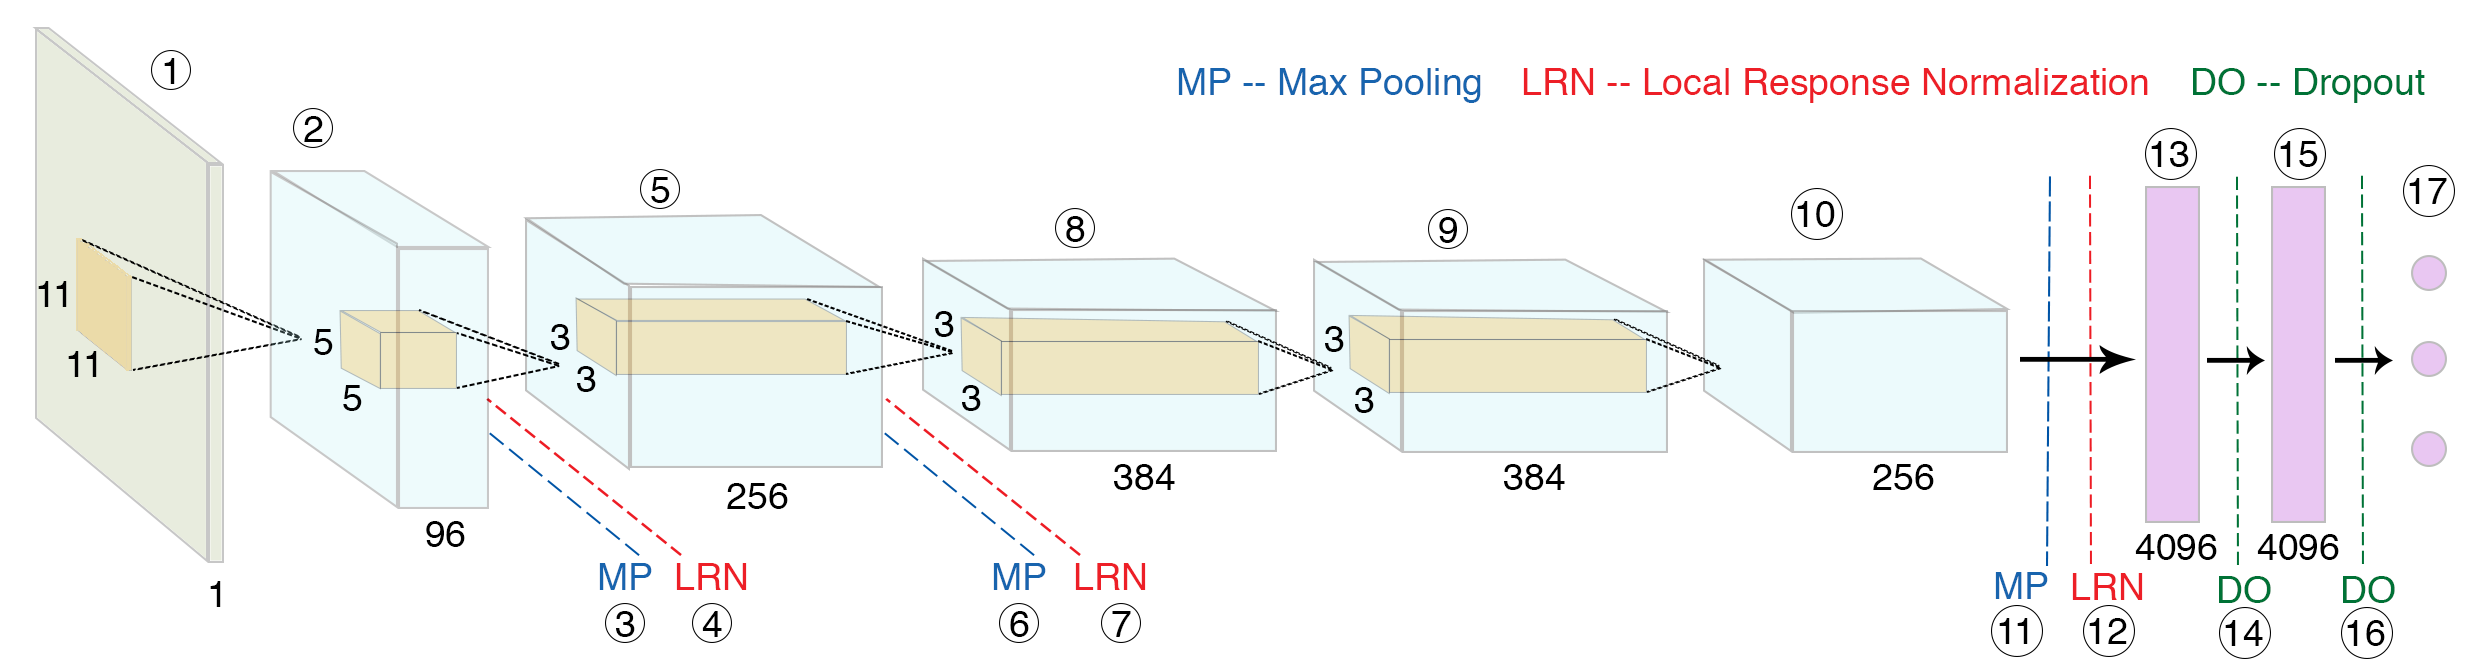
\includegraphics[width = \textwidth, height= 5.2cm]{galmnet_schematic_coloured.pdf}
    \caption{Schematic diagram of \gamornet{}, a CNN optimized to identify whether galaxies are bulge-dominated or disk-dominated. Its architecture, which is based on AlexNet\,\citep{alexnet}, consists of five convolutional layers and three fully connected layers. Between these layers are max-pooling, local response normalization, and dropout layers.t The numbers inside the circles refer to the layer number and corresponding details for each layer can be found by looking up the corresponding layer order number in Table~\ref{tab:network_layers}. }
    \label{fig:galmnet_schematic}
\end{figure*}

\subsection{Initial Training} \label{sec:initial_training}
 Using the two sets of simulations corresponding to the SDSS and CANDELS data sets, we trained two different networks, both with the same structure as described in \S\,\ref{sec:network_description}. Henceforth, we refer to the networks trained on SDSS and CANDELS simulations as \gamornet{}-S and \gamornet{}-C respectively. During the training process, we trained the networks to separate galaxies into three different categories:
\begin{enumerate}[noitemsep]
\item Galaxies with $L_B/L_T < 0.45 $, i.e., disk-dominated.
\item Galaxies with $L_B/L_T > 0.55 $, i.e., bulge-dominated.
\item Galaxies with $ 0.45 \leq L_B/L_T \leq 0.55 $, i.e., indeterminate.
\end{enumerate}
Here, $L_B$ is the luminosity of the bulge component, and $L_T$ is the total luminosity of the galaxy. Since these galaxies are simulated, we used our knowledge of the actual $L_B/L_T$ for each galaxy to train the network.

Of the 100,000 galaxies simulated for each data set, we used $90\%$ for training and the rest for validation. The validation set was used to tune the different hyper-parameters in the network (like the learning rate described in \S\,\ref{sec:network_description}). We use a learning rate of 0.0001 and a batch size of 64, as these lead to $>95\%$ accuracy on the validation set and run-times of $\sim\mathcal{O}(1\mathrm{\,hour})$ on Tesla P100 GPUs. The batch size refers to the number of training samples the network works through before the model's internal parameters are updated

During the training process, we used the categorical cross-entropy loss function and minimized it using the momentum optimizer, which is a variant of SGD and accelerates SGD in the relevant direction besides dampening oscillations during the minimization process. Both SGD and the categorical cross-entropy loss function are described in \S\,\ref{sec:network_description}. 

An ``epoch" of training refers to running all of the training images through the network once. After each epoch of training, we evaluated the value of the loss function and calculated the accuracy on the validation set. The process of calculating the accuracy involves running all of the images in the validation set through the network. Since the output layer in our network is a softmax layer, the output value of each neuron can be interpreted as the network's predicted probability of the galaxy image to belong to the particular category corresponding to that neuron. A galaxy is said to belong to the $L_B/L_T$ category for which the predicted probability is the highest, and the accuracy was calculated as the number of galaxies classified correctly divided by the total number of galaxies. It is important to note here that we used an additional criterion for classifying the real images later on, as described in \S\,\ref{sec:morph_results}.

We trained both the networks until the values of the accuracy and the loss function stabilized and a significant gain in accuracy did not seem probable with further training. This constituted training \gamornet{}-S for 1000 epochs and \gamornet{}-C for 400 epochs. Both learning curves are shown in Figure~\ref{fig:base_network_train}, which shows the accuracy as well as the value of the loss function after each epoch of training. \gamornet{}-S and \gamornet{}-C achieved net accuracies of $93.55\%$ and $88.33\%$, respectively, on the simulated images being used for validation; note that these are simulated images that the network did not ``see" during the process of training. 

\begin{figure*}[htb]
	\begin{center}
    \subfigure[SDSS]{\label{fig:sdss_base_network}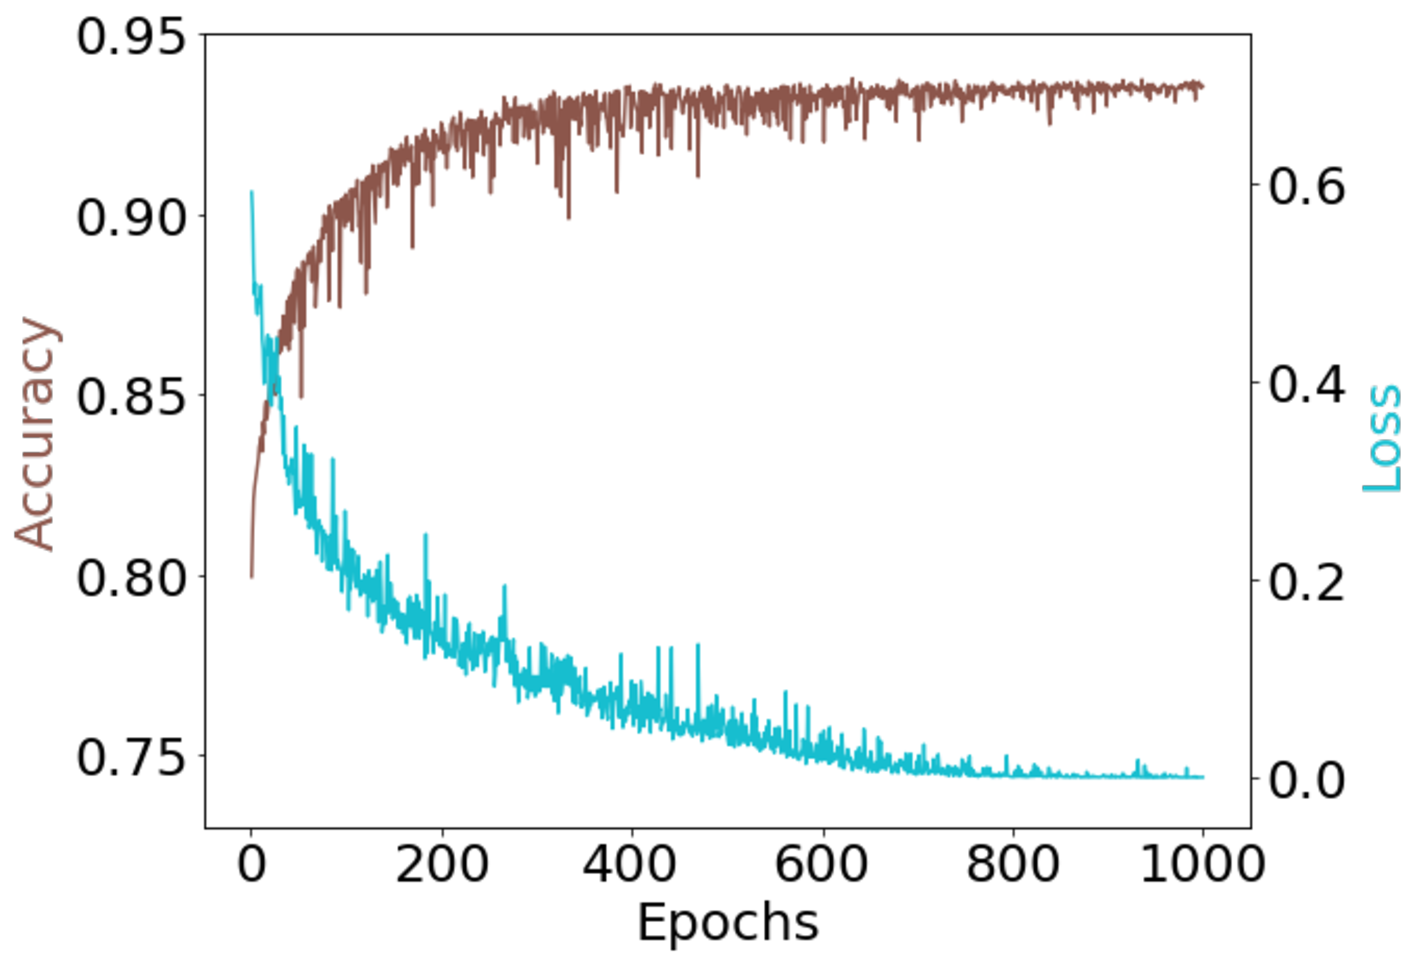
\includegraphics[width=0.45\textwidth]{run_sdssg_2a_acc_loss.pdf}}
    \subfigure[CANDELS]{\label{fig:candels_base_network}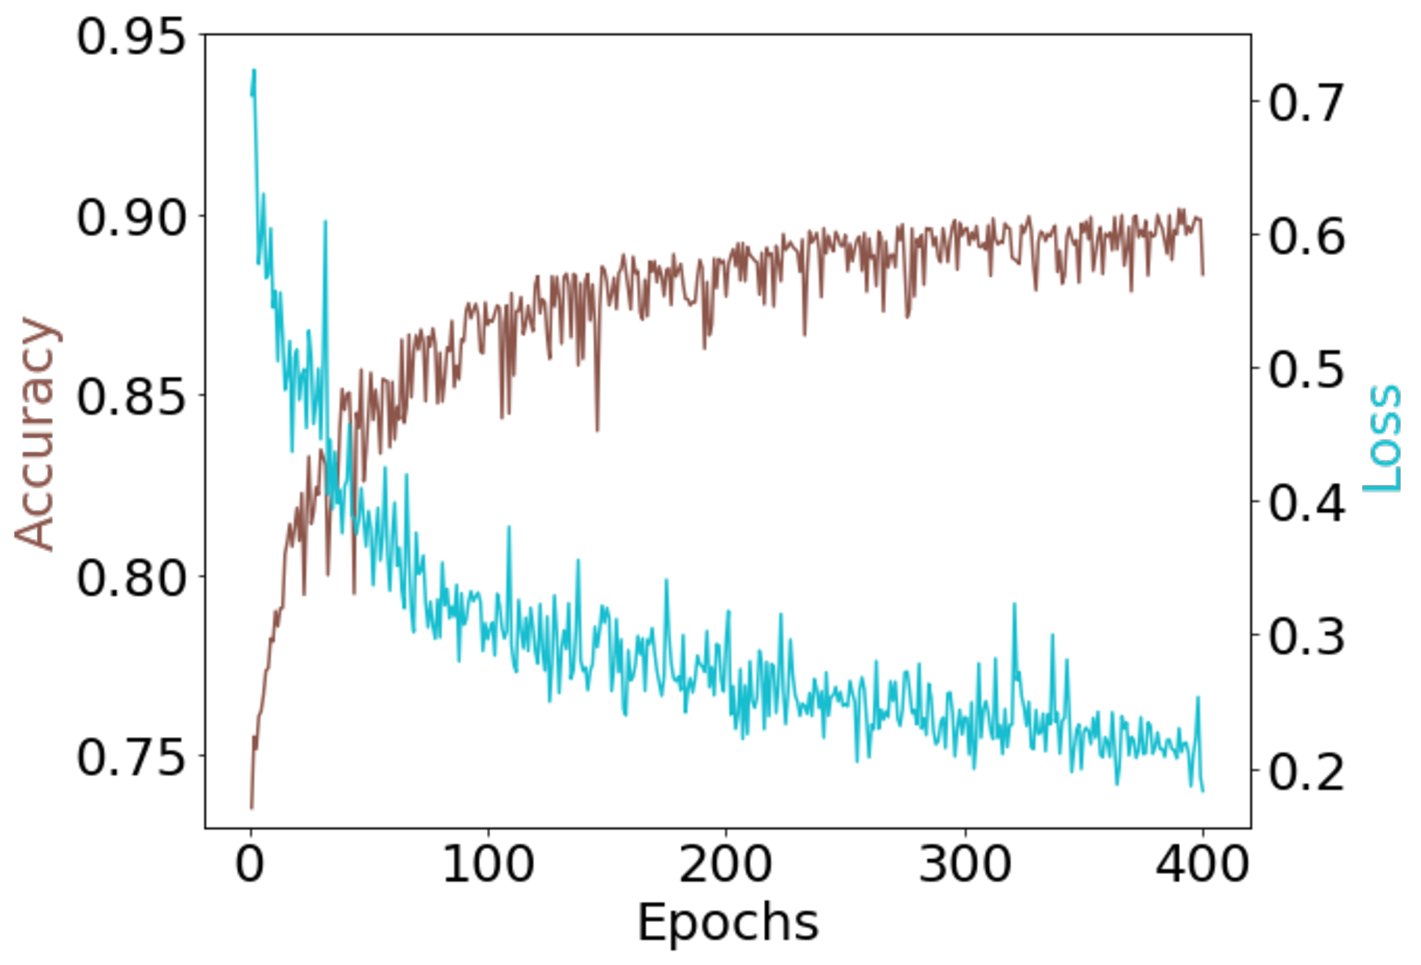
\includegraphics[width=0.45\textwidth]{run_candelsh_2b_acc_loss.pdf}}
  \end{center}
  \caption{Learning curves for the process of training \gamornet{} on simulated galaxy images. The accuracy evaluated on the validation set (brown curves, left axes) and the value of the loss function after each epoch of training (blue curves, right axes) are shown for both \gamornet{}-S and \gamornet{}-C (left and right panels, respectively). \gamornet{}-S achieves an accuracy of $93.55\%$ after 1000 epochs of training, and \gamornet{}-C achieves an accuracy of $88.33\%$ after 400 epochs of training. For more details about the training process, see \S\,\ref{sec:initial_training}.}
  \label{fig:base_network_train}
\end{figure*}

\subsection{Transfer Learning} \label{sec:tf_intro}

\begin{table}[htbp]
  \centering
  \caption{Transfer Learning Parameters \label{tab:tl_para}}
  \begin{tabular}{p{2.5cm}p{2.5cm}p{3.25cm}p{3.25cm}p{1.25cm}}
  \hline
  \hline
  Network & Non-Trainable Layers & Layers Trained from Previous Training & Layers Trained from Scratch & Learning Rate \\
  \hline
  \gamornet{}-S & None & All Convolutional Layers (2,5,8,9,10) & Last 3 Fully Connected Layers (13,15,17) & 0.00001 \\
  \hline
  \gamornet{}-C & First 3 Convolutional Layers (2,5,8) & Last 2 Convolutional Layers + First Fully Connected Layer (9,10,13)& Last 2 fully Connected Layers (15,17) & 0.00001 \\
  \hline
  \multicolumn{5}{p{0.9\textwidth}}{\vskip 0.1cm \small \textsubscript{a} These layers were optimized during the initial training on simulations and then frozen at those values for the transfer learning step.} \\
  \multicolumn{5}{p{0.9\textwidth}}{ \small \texttt{NOTE-} Details of the transfer learning algorithm used for both the SDSS and CANDELS networks. The numbers in parentheses refer to the layer numbers according to Table \ref{tab:network_layers}. The above parameters were chosen by heuristically testing various options and choosing the ones that maximized accuracy, while not showing any signs of over-training.}
  \end{tabular}
\end{table}

CNNs have an extremely large number of free parameters (weights and biases) that need to be tuned during the process of training, and thus, if the size of the training set is not sufficiently large, there is a chance of ``over-fitting" after a certain number of epochs of training. That is, with further training, the accuracy of the network increases on the training data but not on the test data, and hence, the network fails to generalize. 

Transfer learning involves taking a network trained on a particular data set and optimized for a particular task, and re-tuning the weights and biases for a slightly different task or data set. The advantage here is that a much smaller training set can be used to re-tune the network than to train it from scratch. Transfer learning as a data-science concept has been around since the 1990s \citep{Pan2010}, and has been applied to a wide variety of tasks, including image classification\,\citep{zhu2011,Kulis2011,Duan2012}. As an example, transfer learning was recently applied to detect galaxy mergers\,\citep{ml_mergers}, starting from a network that could accurately identify images of everyday objects like cars, cats, dogs, etc.

In the present work, since we want to enable morphological classification even in the absence of a large training set, we use only a small fraction of the SDSS and CANDELS data sets for training. Specifically, we take the network trained on simulations and then re-train it by transfer learning on $\sim25\%$ of the real SDSS and CANDELS galaxy images.

In transfer learning, it is common to freeze the weights and biases in the initial layers of the network (i.e., those close to the input layer), while allowing variations in layers close to the output layer. The logic behind this approach is that, in a CNN, the deeper feature maps identify more complicated features while the earlier layers identify more basic features (like lines, shapes, and edges). Since transfer learning re-trains a network to do a slightly different task than it was initially trained to do, it is the last few layers that need to be re-tuned for the task at hand. At the same time, since the earlier layers correspond to more basic features, we do not expect that they will need re-tuning. We heuristically tested a combination of the various options mentioned above, and chose the one that maximized accuracy, while not showing any signs of over-training. The details of the transfer learning method used in both cases are summarized in Table~\ref{tab:tl_para}.

For the SDSS data, we have access to estimates of $L_B/L_T$ for each galaxy from \citet{simard_11}, wherein each galaxy was fitted with an $n=4$ bulge and an $n=1$ disk component. We used this as the ``ground truth'' for separating galaxies into the three categories defined in \S~\ref{sec:initial_training}. We randomly selected 10,000 galaxies from each category to make up our transfer learning training data set; this constitutes about a quarter of the full SDSS sample. We found that during transfer learning, it is important to have an equal number of galaxies from each category in the training set because otherwise, the network attempts to maximize accuracy in the category with more samples at the cost of other categories. Since both our samples have many more disk-dominated than bulge-dominated galaxies, a randomly selected training set would result in a very high accuracy in classifying disk-dominated galaxies but a very low accuracy in classifying bulge-dominated galaxies. Using the configuration given in Table~\ref{tab:tl_para}, we trained \gamornet{}-S for 300 epochs.

\begin{figure}[hbt]
    \centering
    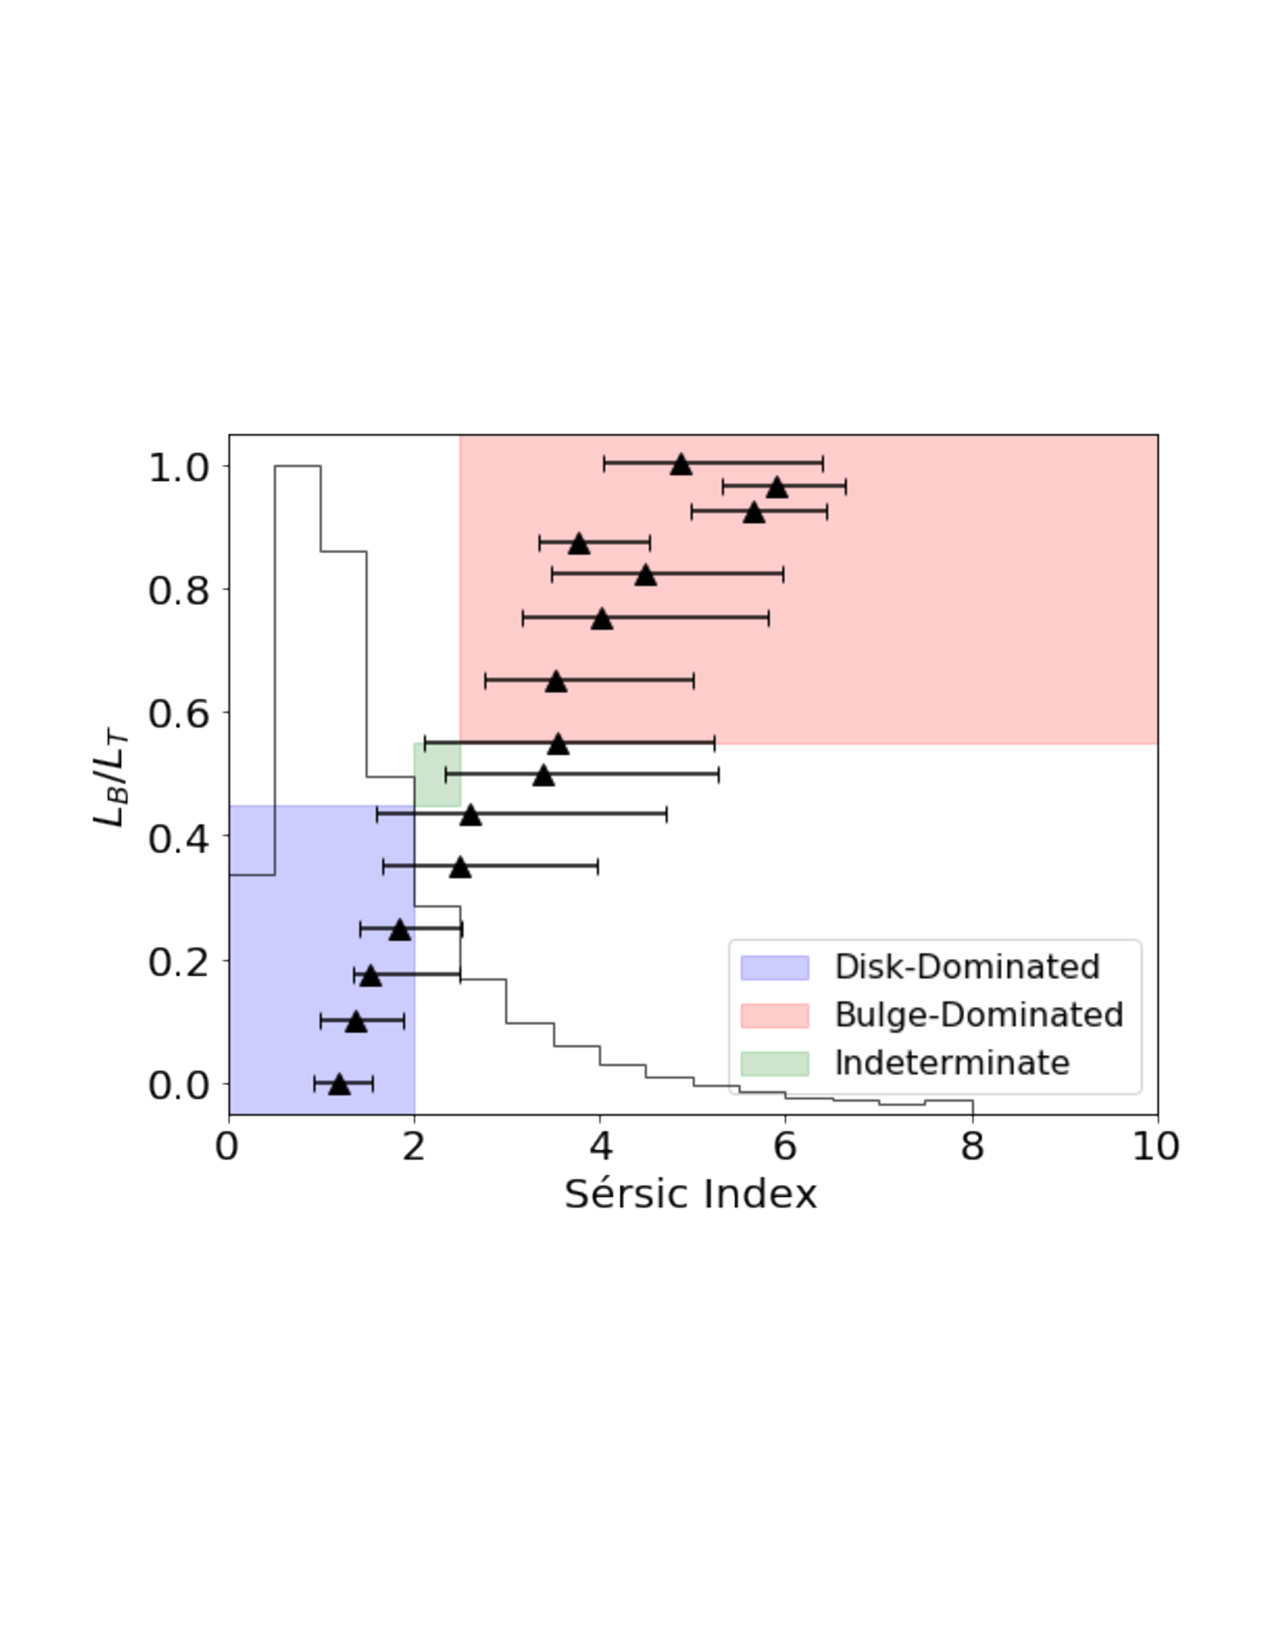
\includegraphics[width=0.55\textwidth]{btr_si.pdf}
    \caption{ The triangles show the input bulge-to-total ratio ($L_B/L_T$) versus fitted \sersic{} index for the galaxies simulated by \citeauthor{simmons_08} (\citeyear{simmons_08}; adapted from the lowest panel in their Figure 19). The plotted points are the median of each bin's distribution, and the error bars mark the central 68\% of sources in the bin. The shaded regions correspond to our definitions of the three output classes used by \gamornet{}-C. The histogram shows the distribution of the \sersic{} index for all the galaxies in our CANDELS sample, most of which are disk-dominated (see \S\,\ref{sec:data}). Clearly, all galaxies with $n<2$ are truly disk-dominated (i.e., have $L_B/L_T < 0.45$) but, because of the spread in \sersic{} indices, some disk-dominated or intermediate galaxies may get misclassified as bulge-dominated. Although a higher $n$ threshold (for, e.g., $n \sim 6$) would lead to a purer bulge-dominated sample, for reasons mentioned in \S\,\ref{sec:tf_intro}, it would make the transfer learning sample insufficiently small. Note that readers can choose different bin boundaries, doing their own transfer learning step on the simulation-trained network made available via \S\,\ref{sec:ap:gamornet_trained_models}}
    \label{fig:si_lb_lt}
\end{figure}{}
    
For the CANDELS data, no two-component bulge-disk decompositions were available in the literature. Thus, we translated the \sersic{} indices from \citet{vdw_12} into the three classifications used by \gamornet{} using results from \citet{simmons_08}, who analyzed CANDELS-depth HST ACS simulations of bulge+disk galaxies. The authors fitted single \sersic{} profiles to their simulations in order to find the correspondence between \sersic{} index and actual $L_B/L_T$. Guided by their result in the redshift bin $z=1.075$ (see their Fig.~19), appropriate for the CANDELS galaxies we wish to classify, we define galaxies with $n < 2.0$ as disk-dominated, $n > 2.5$ as bulge-dominated, and $ 2.0 \leq n \leq 2.5$ as indeterminate.
    
To illustrate these choices, we reproduce in Figure \ref{fig:si_lb_lt} the \citet{simmons_08} results, specifically, the range in \sersic{} index corresponding to different $L_B/L_T$ values for the simulated galaxies. The three broad classifications assigned by \gamornet{}-C --- disk-dominated, indeterminate, and bulge-dominated --- are shown as shaded regions. There is no unique or perfect way to go from \sersic{} index to $L_B/L_T$; although, the choice of $n<2$ is pretty clean, i.e., all such galaxies have $L_B/L_T < 0.45$ and are disk-dominated. For $n>2.5$, most galaxies are bulge-dominated (i.e., have $L_B/L_T > 0.55$) as is evident from the top-right portion of the figure; although, a few disk-dominated galaxies with $L_B/L_T \sim 0.4$ may be incorrectly included in that category. 
    
A higher $n$ threshold (for, eg., $n\sim6$) leads to a purer bulge-dominated sample, but drastically reduces the number of bulge-dominated galaxies available for transfer learning, as is evident from the histogram shown in Figure \ref{fig:si_lb_lt}. As mentioned previously, we need roughly equal numbers of galaxies in each bin for the training process during transfer learning, and thus, the upper limit on the total number of galaxies available for training is set by the size of the least populous bin. The above choices ensure a sufficient number of galaxies in each category (needed for the transfer learning step) and produce statistically acceptable classifications. Readers can set these boundaries differently, as appropriate to their science goals, using \gamornet{}-C models trained only on the bulge + disk simulations made publicly available via \S\,\ref{sec:ap:gamornet_trained_models}. Instructions on how to train these models for transfer learning are available in the GitHub repository.
    
Using the above definitions of the three classes, we re-trained the simulation-trained \gamornet{}-C for 75 epochs using the Transfer Learning configuration in Table~\ref{tab:tl_para}; note that only the weights and biases in the last two of the total five convolutional layers are adjusted during the transfer learning step. For this process, we used 2400 galaxies from each of the three morphological categories, or about a quarter of the total CANDELS sample.

\begin{table}[htbp]
  \centering
  \caption{Classification Probabilities for 82,547 SDSS Galaxies}
  \label{tab:lt_sdss}
  \begin{tabular}{ccccccc}
  \hline
  \hline
  ObjID\textsuperscript{a} & R.A. & Decl. & Disk & Bulge & Indetermi- & Classification \\
   & (deg) & (deg) & Prob. & Prob. & nate Prob.& \\ 
  \hline
  587722953\ldots & 237.4210352 & 0.2367580 & 0.1356 & 0.4439 & 0.4205 & indeterminate \\
  587722981\ldots & 202.6811651 & -1.0804622 & 1.0000 & 0.0000 & 0.0000 & disk-dominated\\
  587722982\ldots & 219.5687676 & -0.3497467 & 0.9384 & 0.0001 & 0.0615 & disk-dominated\\
  587722983\ldots & 213.2606435 & 0.1463757 & 0.9977 & 0.0000 & 0.0023 & disk-dominated\\
  587722983\ldots & 216.5747982 & 0.1543351 & 0.0590 & 0.7170 & 0.2240 & indeterminate\\
  \vdots & \vdots &\vdots &\vdots &\vdots &\vdots &\vdots\\
  \hline
  \multicolumn{7}{p{0.92\textwidth}}{\vskip 0.01cm \small \textsuperscript{a}These are pre-DR8 ObjIDs. Complete object IDs are not mentioned here for stylistic purposes.} \\
  \multicolumn{7}{p{0.92\textwidth}}{\small \texttt{NOTE-} \gamornet{}-S classification probabilities (of being disk-dominated, bulge-dominated, or indeterminate) and final classification for all the galaxies in our SDSS test sample. This table is published in its entirety as a part of the public data release (Appendix \ref{sec:ap:prob_tables}). The first five entries are shown here for guidance regarding its form and content.}
  \end{tabular}
  \end{table}

  \begin{table}[htbp]
    \centering
    \caption{Classification Summary for 82,547 SDSS Galaxies \label{tab:sdss_results}}
        \begin{tabular}{|>{\centering\arraybackslash}p{3cm}|>{\centering\arraybackslash}p{2.25cm}|>{\centering\arraybackslash}p{2.0cm}|>{\centering\arraybackslash}p{2.0cm}|}
        \hline
        \hline
        \multicolumn{4}{|c|}{Predictions:- Disks: 47,656 $|$ Bulges: 7963 $|$ Indeterminate: 26,928}\\
        \hline
        \hline
        \multicolumn{2}{|c|}{} & \multicolumn{2}{c|}{\gamornet{}-S classifications} \\
        \cline{3-4}
        \multicolumn{2}{|c|}{} & Disks & Bulges \\
        \hline
        \citet{simard_11}   & Disks & 47,526 & 329\\ \cline{2-4} classifications & Bulges & 94 & 7552 \\
        \hline
        \hline
        \multicolumn{4}{|c|}{Percentages} \\
        \hline
        \multicolumn{3}{|c|}{\gamornet{}-classified disks that SC\textsuperscript{a} also classified as disks} & $99.73\%$\\
        \multicolumn{3}{|c|}{\gamornet{}-classified disks that SC\textsuperscript{a} classified as bulges} & $0.20\%$\\
        \hline
        \multicolumn{3}{|c|}{\gamornet{}-classified bulges that SC\textsuperscript{a} also classified as bulges} & $94.84\%$\\
        \multicolumn{3}{|c|}{\gamornet{}-classified bulges that SC\textsuperscript{a} classified as disks} & $4.13\%$\\
        \hline
        \multicolumn{3}{|c|}{Total percentage of galaxies misclassified} & $0.7\%$\\
        \hline
        \multicolumn{4}{p{0.82\textwidth}}{\vskip 0.01cm \small \textsuperscript{a}SC refers to \citet{simard_11} classifications.} \\
        \multicolumn{4}{p{0.82\textwidth}}{\small \texttt{NOTE-} Results of running the entire SDSS test set of 82,547 galaxies through \gamornet{}-S. Values in the top section refer to the number of galaxies in each category as predicted by \gamornet{}-S with respect to the \citet{simard_11} classifications. For example, the top-left cell value of 47,526 means that out of the 47,656 predicted disks, 47,526 are also classified as disks by \citet{simard_11}.}
        \end{tabular}
    \end{table}

\section{Results} \label{sec:results}
\subsection{Morphology Results}\label{sec:morph_results}
After using about a quarter of the images for transfer learning, the remaining 82,547 galaxies in the SDSS sample were used as our test set. Since \gamornet{}'s output layer consists of three softmax neurons whose output values sum to $1$, each value can be interpreted as the probability that a galaxy belongs to that $L_B/L_T$ category. These probability values are the primary output of \gamornet{}. However, in order to compare our results with previous classifications and keeping in mind situations that necessitate rigid classifications, we transform the probability values into classifications.

After some experimentation, we arrived at this decision tree for classification:
\begin{enumerate}[noitemsep]
\item Disk-dominated when \gamornet{}-S reports $\geq 80\%$ probability that $L_B/L_T < 0.45$.
\item Bulge-dominated when \gamornet{}-S reports $\geq 80\%$ probability that $L_B/L_T > 0.55$.
\item Otherwise, indeterminate.
\end{enumerate}
This is slightly different than the criterion we used for the initial training, as those galaxies were idealized, and the classifications were unambiguous. For the real galaxies, simply taking the highest probability neuron, including probabilities below 80\%, made the classifications far less accurate. Requiring a threshold of 80\% greatly improved the classification accuracy at the expense of increasing the number of indeterminate galaxies.


For each galaxy, we have access to its bulge-to-total ratio, i.e., $L_B/L_T$ value from \citet{simard_11}, which we consider to be the ``true" value. For mapping $L_B/L_T$ to a classification of being bulge- or disk-dominated, we used the same criterion as during the initial training, outlined at the beginning of \S\,\ref{sec:initial_training}.

Individual morphological classifications by \gamornet{}-S are reported in Table~\ref{tab:lt_sdss} and Table~\ref{tab:sdss_results} compares the \gamornet{}-S and \citet{simard_11} classifications of SDSS galaxies. Assuming the latter are ``true", for disk-dominated galaxies, we achieved an accuracy of 99.7\% and for bulge-dominated galaxies, we achieved an accuracy of 94.8\%, resulting in a net misclassification rate of 0.7\%. A total of 26,928 galaxies, or $\sim 32$\% of the SDSS test set, were found to have indeterminate morphologies.

\begin{table}[htbp]
  \centering
  \caption{Classification Probabilities for 21,746 CANDELS galaxies \label{tab:lt_candels}}
  \begin{tabular}{cccccccc}
  \hline
  \hline
  Field & ID\textsuperscript{a} & R.A. & Decl. & Disk & Bulge & Indetermi- & Classification\\
  & & (deg) & (deg) & Prob. & Prob. & nate Prob.& \\
  \hline
  GOODSN & 19 & 189.146484 & 62.095764 & 0.3356 & 0.3372 & 0.3272 & indeterminate\\
  GOODSN & 32 & 189.131485 & 62.097328 & 0.3762 & 0.2722 & 0.3516 & disk-dominated\\
  GOODSN & 63 & 189.117432 & 62.101723 & 0.3709 & 0.2877 & 0.3414 & disk-dominated\\
  GOODSN & 68 & 189.149979 & 62.101768 & 0.4039 & 0.1798 & 0.4163 & indeterminate\\
  GOODSN & 72 & 189.143295 & 62.102295 & 0.3006 & 0.3312 & 0.3683 & indeterminate\\
  \vdots & \vdots &\vdots &\vdots &\vdots &\vdots &\vdots &\vdots\\
  \hline
  \multicolumn{8}{p{0.9\textwidth}}{\vskip 0.01cm \small ID refers to the IDs assigned by the CANDELS team\,\citep{candels_1,candels_2}}\\
  \multicolumn{8}{p{0.9\textwidth}}{\small \texttt{NOTE-} \gamornet{}-C classification probabilities (of being disk-dominated, bulge-dominated, or indeterminate) and final classification for all the galaxies in our CANDELS test sample. This table is published in its entirety as a part of the public data release (Appendix \ref{sec:ap:prob_tables}). The first five entries are shown here for guidance regarding its form and content.}\\
  \end{tabular}
\end{table}

\begin{table}[htbp]
  \centering
  \caption{Classification Summary for 21,746 CANDELS Galaxies \label{table:candels_results}}
  \begin{tabular}{|>{\centering\arraybackslash}p{4cm}|>{\centering\arraybackslash}p{2cm}|>{\centering\arraybackslash}p{2.0cm}|>{\centering\arraybackslash}p{2.0cm}|}
      \hline
      \hline
      \multicolumn{4}{|c|}{Predictions:- Disks: 12,549 $|$ Bulges: 580 $|$ Indeterminate: 8617}\\
      \hline 
      \hline
       \multicolumn{2}{|c|}{} & \multicolumn{2}{c|}{\gamornet{}-C classifications} \\
       \cline{3-4}
       \multicolumn{2}{|c|}{} & Disks & Bulges \\
       \hline
       \citet{vdw_12}  & Disks & 11,524 & 121 \\ \cline{2-4} classifications & Bulges & 992 & 456 \\
       \hline
       \hline
       \multicolumn{4}{|c|}{Percentages} \\
       \hline
       \multicolumn{3}{|c|}{\gamornet{}-classified disks that VdwC\textsuperscript{a} also classified as disks } & 91.83\%\\
       %\hline
       \multicolumn{3}{|c|}{\gamornet{}-classified disks that VdwC\textsuperscript{a} classified as bulges} & 7.90\%\\
       \hline
       \multicolumn{3}{|c|}{\gamornet{}-classified bulges that VdwC\textsuperscript{a} also classified as bulges} & 78.62\%\\
       %\hline
       \multicolumn{3}{|c|}{\gamornet{}-classified bulges that VdwC\textsuperscript{a} classified as disks} & 20.86\%\\
       \hline
       \multicolumn{3}{|c|}{Total percentage of galaxies misclassified} & 5.3\%\\
       \hline
       \multicolumn{4}{p{0.82\textwidth}}{\vskip 0.1cm \small \textsuperscript{a}\citet{vdw_12} Classifications}\\
       \multicolumn{4}{p{0.82\textwidth}}{\small \texttt{NOTE-}Results of running the entire CANDELS test set of 21,746 galaxies through \gamornet{}-C. Values in the top section refer to the number of galaxies in each category as predicted by \gamornet{}-C with respect to the \citet{vdw_12} classifications. For example, the top-left cell value of 11,524 means that out of the 12,549 predicted disks, 11,524 are also classified as disks by \citet{vdw_12}.}\\
  \end{tabular}
  \end{table}


For the CANDELS data set, there were 21,746 galaxies in the test set. We classified these using \gamornet{}-C and, again, experimented with thresholds for the final neuron values in order to arrive at an acceptable balance between accuracy and fraction with indeterminate morphologies. The thresholds for the CANDELS classification (which are different from those adopted for the SDSS data) are:
\begin{enumerate}[noitemsep]
    \item Bulge-dominated if \gamornet{}-C reports $\geq 55\%$ probability that $L_B/L_T > 0.55 $.
    \item Disk-dominated if \gamornet{}-C reports $\geq 36\%$ probability that $L_B/L_T < 0.45 $ {\it and} this probability exceeds the probabilities of $L_B/L_T > 0.55 $, $0.45 \leq L_B/L_T \leq 0.55 $.
    \item Otherwise, indeterminate.
\end{enumerate}
The choice of these confidence thresholds and their impact on the results is discussed later in this section. 

Table~\ref{tab:lt_candels} reports the individual morphological classifications by \gamornet{}-C, and
Table~\ref{table:candels_results} compares these to the results of \citet{vdw_12}. From the \sersic{} index of each galaxy \citep{vdw_12}, we derive its $L_B/L_T$ following \citet{simmons_08} as described in \S\,\ref{sec:tf_intro}. Thereafter, we map these values to a classification of being bulge- or disk-dominated using the same criterion as we did during initial training, as described in \S\,\ref{sec:initial_training}. Assuming these as the ``true" classifications, \gamornet{}-C has an accuracy of 91.8\% for disk-dominated galaxies and 78.6\% for bulge-dominated galaxies, or a net misclassification rate of 5.3\%. A total of 8617 galaxies were classified in the indeterminate category, which is $\sim39$\% of the CANDELS test set. 

The misclassification rate of CANDELS galaxies is higher than that of SDSS galaxies. To find out why, we investigated various relevant statistics for the misclassified galaxies. The two most significant variables were the S/N and the half-light radius (taken from \citealp{vdw_12}). Figure~\ref{fig:candels_misclf} shows the distribution of both the correctly classified and misclassified galaxies over these parameters. Although both the misclassified and correctly classified galaxies are distributed similarly over S/N, the misclassified population peaks much more sharply at a lower S/N, showing that a much larger fraction of the misclassifed sample has a low S/N compared to the correctly classified fraction. Similarly, a much larger fraction of the misclassified sample has low values of $r_e$ compared to the correctly classified galaxies. Therefore, we conclude that the misclassified galaxies are essentially galaxies with a small half-light radius comparable to the PSF and/or a low S/N, and thus, it is inherently difficult for \gamornet{}-C to correctly classify these galaxies. The misclassified population in the SDSS data set also peaks more sharply at a lower value of $r_e$ compared to the correctly classified galaxies; although, we have poor statistics for this, as the misclassification rate is $<1\%$. 


\begin{figure*}[htb]
	\begin{center}
    \subfigure[]{\label{fig:candels_sn}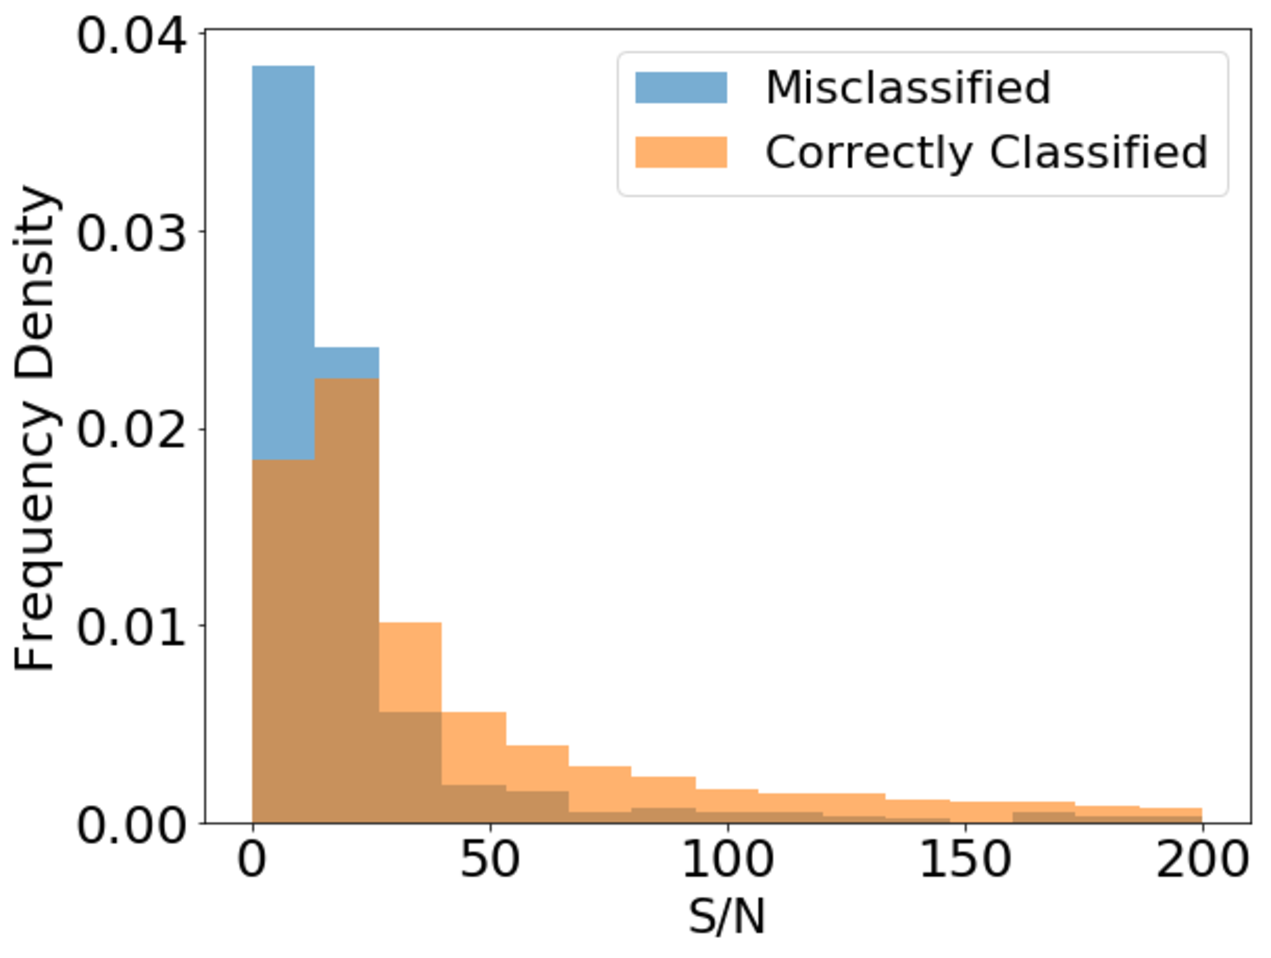
\includegraphics[width=0.50\textwidth]{candels_sn.pdf}}
    \subfigure[]{\label{fig:candels_re}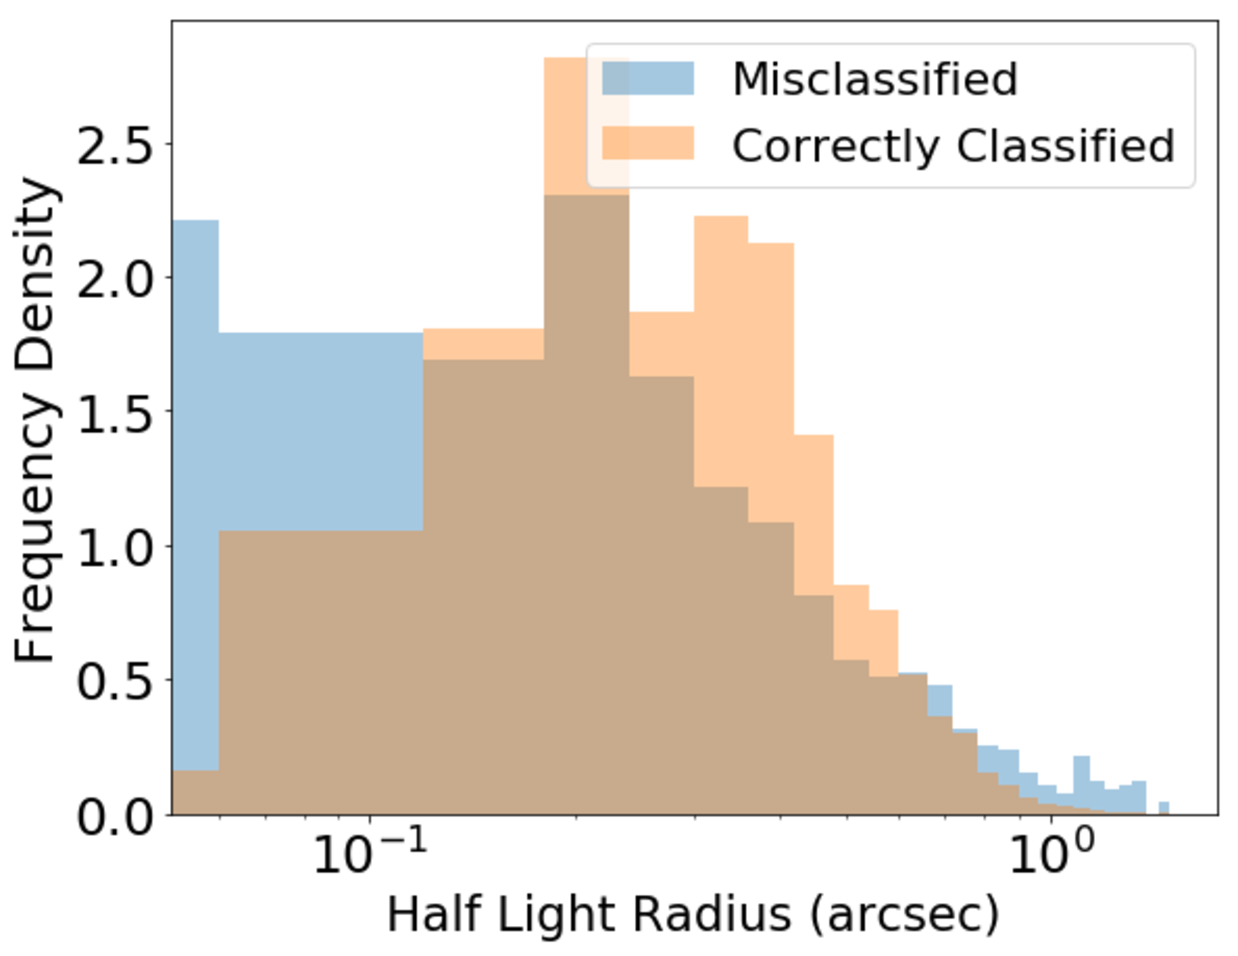
\includegraphics[width=0.48\textwidth]{candels_re.pdf}}
  \end{center}
  \caption{The normalized distribution of correctly classified and misclassifed CANDELS galaxies in the test set as a function of the signal-to-noise ratio (S/N) and half-light radius ($r_e$). Both plots show that compared to the correctly classified galaxies, a higher fraction of the misclassified galaxies have a low S/N ratio and/or small $r_e$. `Frequency density' refers to the number counts normalized to form a probability density.}
  \label{fig:candels_misclf}
\end{figure*}


\begin{figure*}[htb]
	\begin{center}
    \subfigure[]{\label{fig:sdss_unclass_threshold}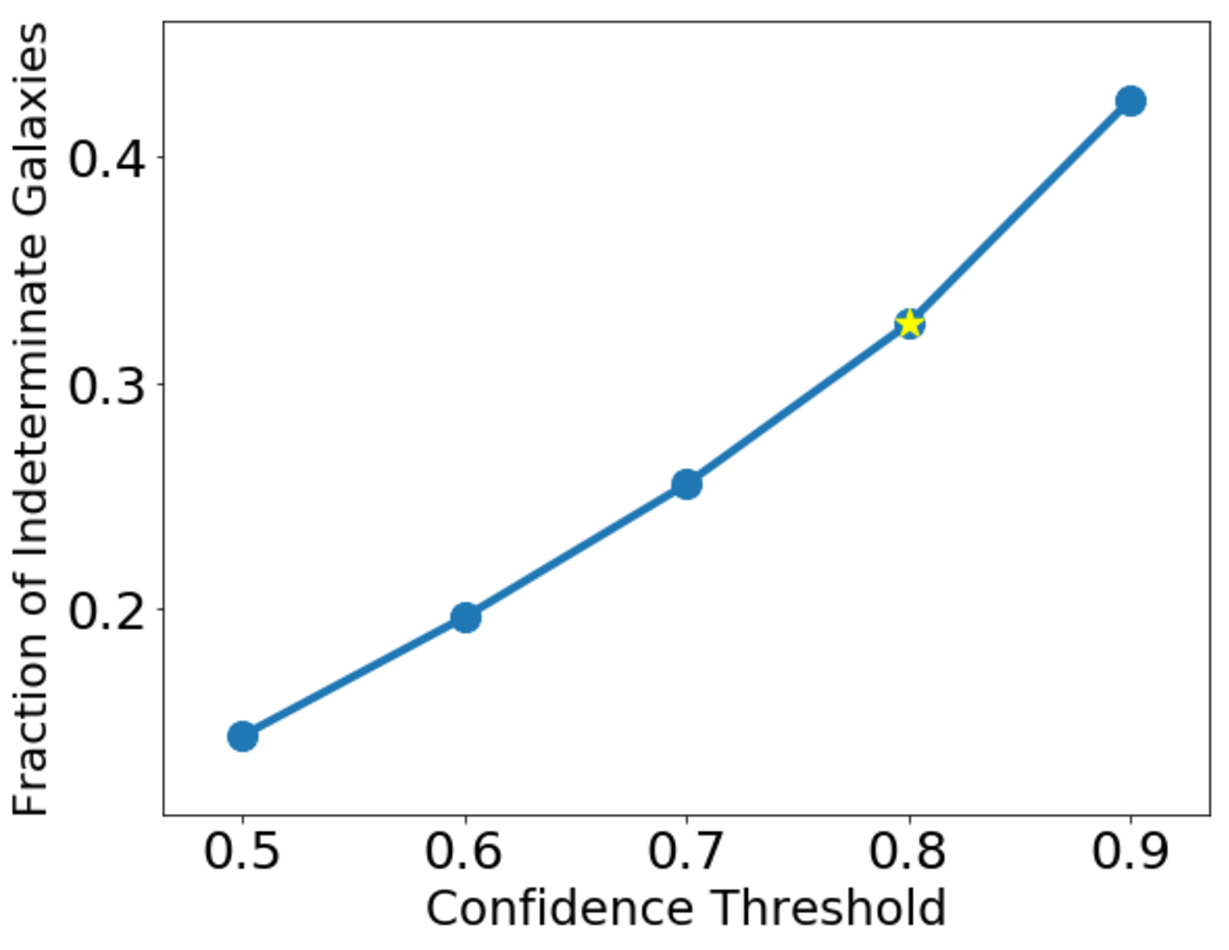
\includegraphics[width=0.41\textwidth]{sdss_unclass_threshold.pdf}}
    \subfigure[]{\label{fig:sdss_acc_threshold}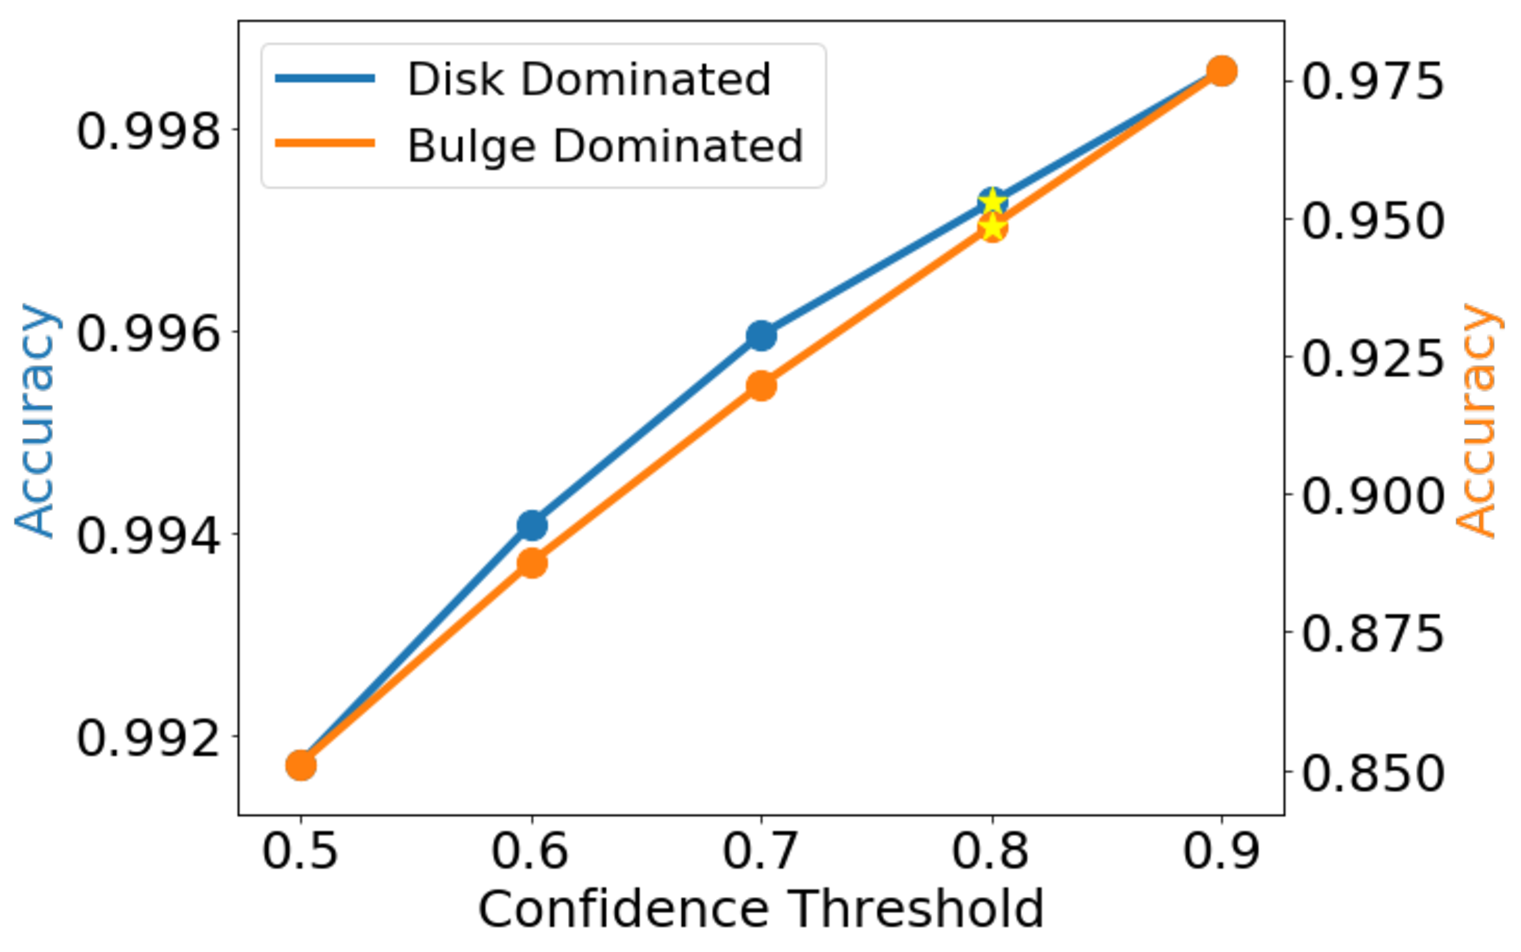
\includegraphics[width=0.50\textwidth]{sdss_acc_threshold.pdf}}
  \end{center}
  \caption{Relation of confidence threshold to completeness and accuracy of classification, for the SDSS data set. Left (a): The fraction of indeterminate galaxies increases with increasing confidence threshold.  Right (b): The accuracy of both disk-dominated (blue line, left axis) and bulge-dominated (orange line, right axis) classifications increases with increasing confidence threshold. We decided on a confidence threshold of 0.8 (or 80\%) for \gamornet{}-S (star in both plots) as the optimal compromise between accuracy and completeness.}
  \label{fig:sdss_threshold}
\end{figure*}


\begin{figure*}[htb]
	\begin{center}
    \subfigure[]{\label{fig:candels_acc_threshold_disk}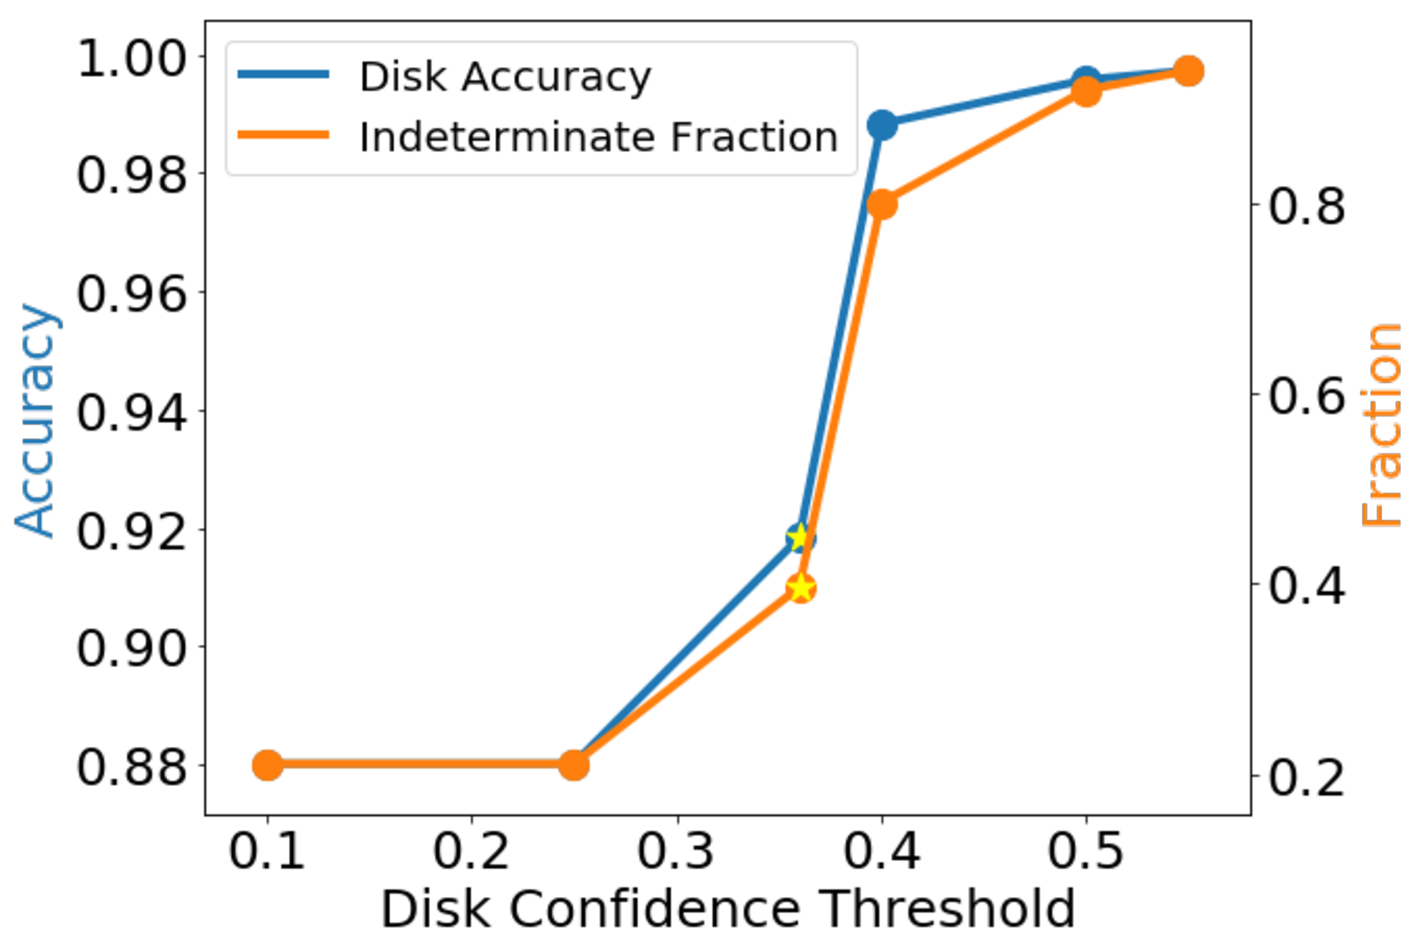
\includegraphics[width=0.45\textwidth]{candels_acc_threshold_disk.pdf}}
    \subfigure[]{\label{fig:candels_acc_threshold_ellips}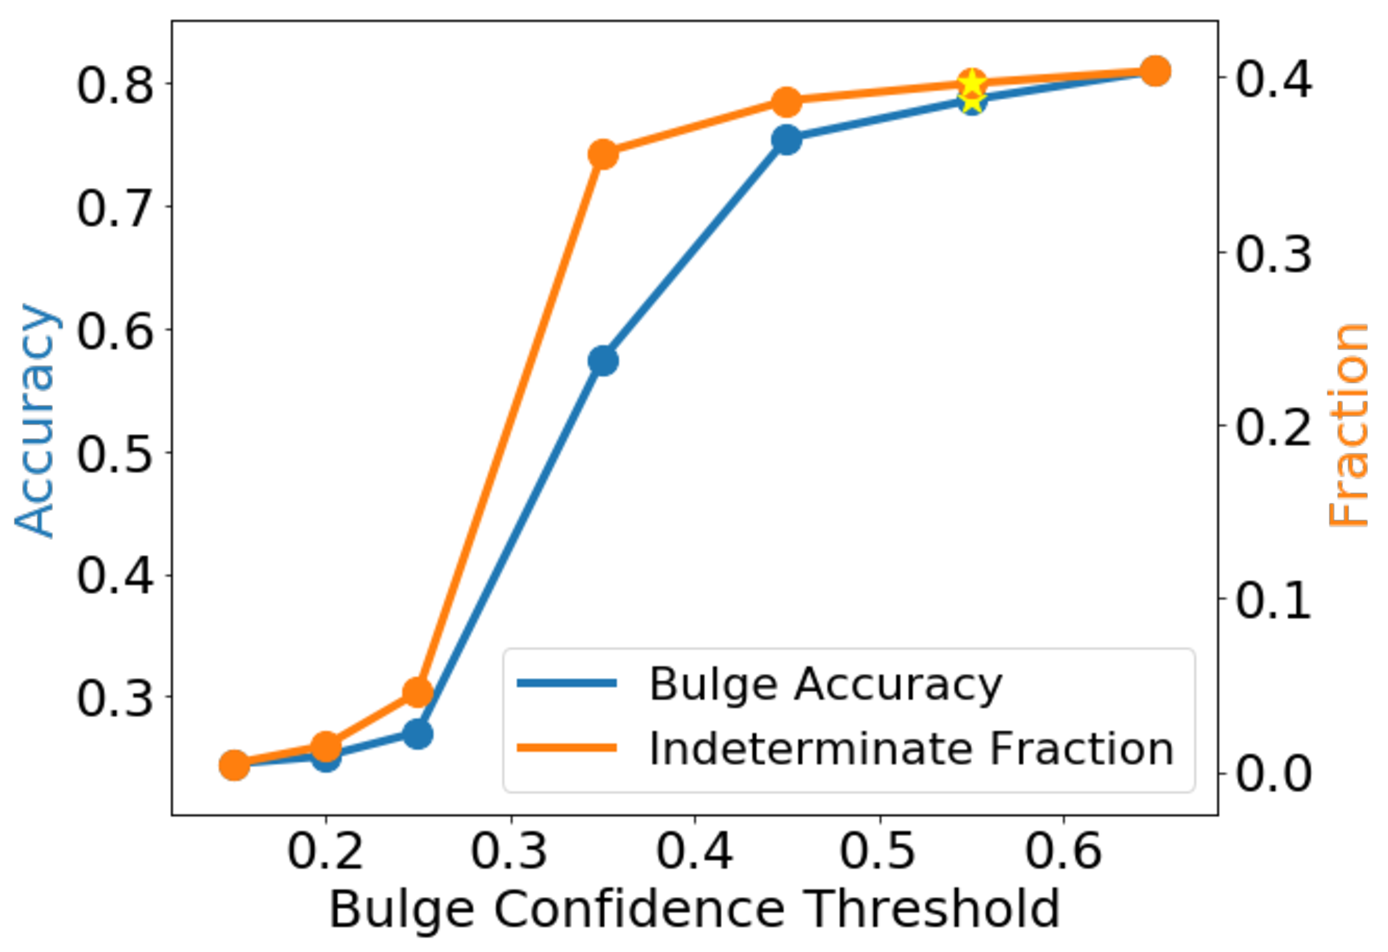
\includegraphics[width=0.45\textwidth]{candels_acc_threshold_ellips.pdf}}
  \end{center}
  \caption{Relation of confidence threshold to the accuracy (blue lines, left axes) and completeness (orange lines, right axes) of \gamornet{}-C classification of the CANDELS data set. Stars denote the adopted confidence thresholds.
  Left (a): For the chosen disk confidence threshold of 0.36, provided the probability of being disk-dominated exceeds the probabilities of being bulge-dominated or indeterminate, the classification accuracy is better than $92\%$ and the indeterminate fraction $<$40\%.
  Right (b): For the chosen bulge confidence threshold of 0.55, we obtain an accuracy of $>$80\% and indeterminate fraction $<$40\%. }
  \label{fig:candels_threshold}
\end{figure*}

The choice of the confidence threshold values to classify a galaxy as bulge- or disk-dominated primarily affects two parameters: the misclassification rate and the number of indeterminate galaxies. Having a high confidence threshold results in a low misclassification rate but a high number of indeterminate galaxies, and vice-versa. We show in Figure~\ref{fig:sdss_threshold} how changing the value of the confidence threshold affects the number of indeterminate galaxies and the accuracy of both the bulge- and disk-dominated galaxies for the SDSS sample. We chose a threshold value of 0.8 or $80\%$ but as the figure shows, even with a threshold of 60\%, it is possible to get $> 85\%$ accuracy for both bulge- and disk-dominated galaxies with an indeterminate fraction as low as $\sim 20\%$.

For the CANDELS data set, setting a common/joint threshold as high as we did for the SDSS data led to most of the data being classified as indeterminate. Thus, we use separate confidence thresholds for the disk and bulge classifications, and the variation of the indeterminate fraction and accuracy with both thresholds is shown in Figure~\ref{fig:candels_threshold}. We chose the final threshold values of 0.36 and 0.55 for the disk- and bulge-dominated galaxies, respectively, as a compromise between the two competing requirements of having a low indeterminate fraction and high accuracy. 

For our choice of confidence thresholds, the indeterminate fraction is $> 25\%$ of the test set for both SDSS and CANDELS. This indeterminate fraction consists of two kinds of galaxies: those with intermediate bulge-to-total ratios (i.e., $0.45 \leq L_B/L_T \leq 0.55$) and those for which the network is not confident enough to make a prediction, because of low S/Ns and/or small sizes. For comparison, \citet{powell_17} used GALFIT to do single \sersic{} fits to 4479 GOODS-S and GOODS-N galaxies; they found that $\sim 38\%$ of the population could not be classified due to poor fits ($\chi^2 > 1.5$) or galaxies having $2.0 < n < 2.5$. Similarly, large fractions of Galaxy Zoo classifications have $\lesssim 80\%$ agreement among classifiers \citep{land_2008}. Thus, even with stringent confidence threshold values, \gamornet{} is able to match the indeterminate fraction of traditional studies. 

The choice of the confidence threshold is arbitrary and should be chosen appropriately for the particular task at hand. Toward this end, Figures \ref{fig:sdss_threshold} and \ref{fig:candels_threshold} can be used to asses the trade-off between accuracy and completeness for both the samples. We have emphasized accuracy over completeness, since we have very large samples already and can show that the misclassified objects simply have lower S/Ns and/or are too compact to classify accurately.

\vspace{1.0cm}

\subsection{Color - Mass Results}\label{sec:cm_results}
In this section, we study the quenching of star formation in  $z\sim0$ (SDSS) and $z\sim1$ (CANDELS) galaxies by examining their color-mass diagrams constructed using the morphological classifications obtained in \S\,\ref{sec:morph_results}. Refer to \S\,\ref{sec:data} for details about the calculation of colors, masses, and sSFR for both samples. 

\begin{figure*}[htbp]
	\begin{center}
	\begin{tabular}{ll}
    \subfigure[Disk-dominated Galaxies]{\label{fig:sdss_disk_scatter}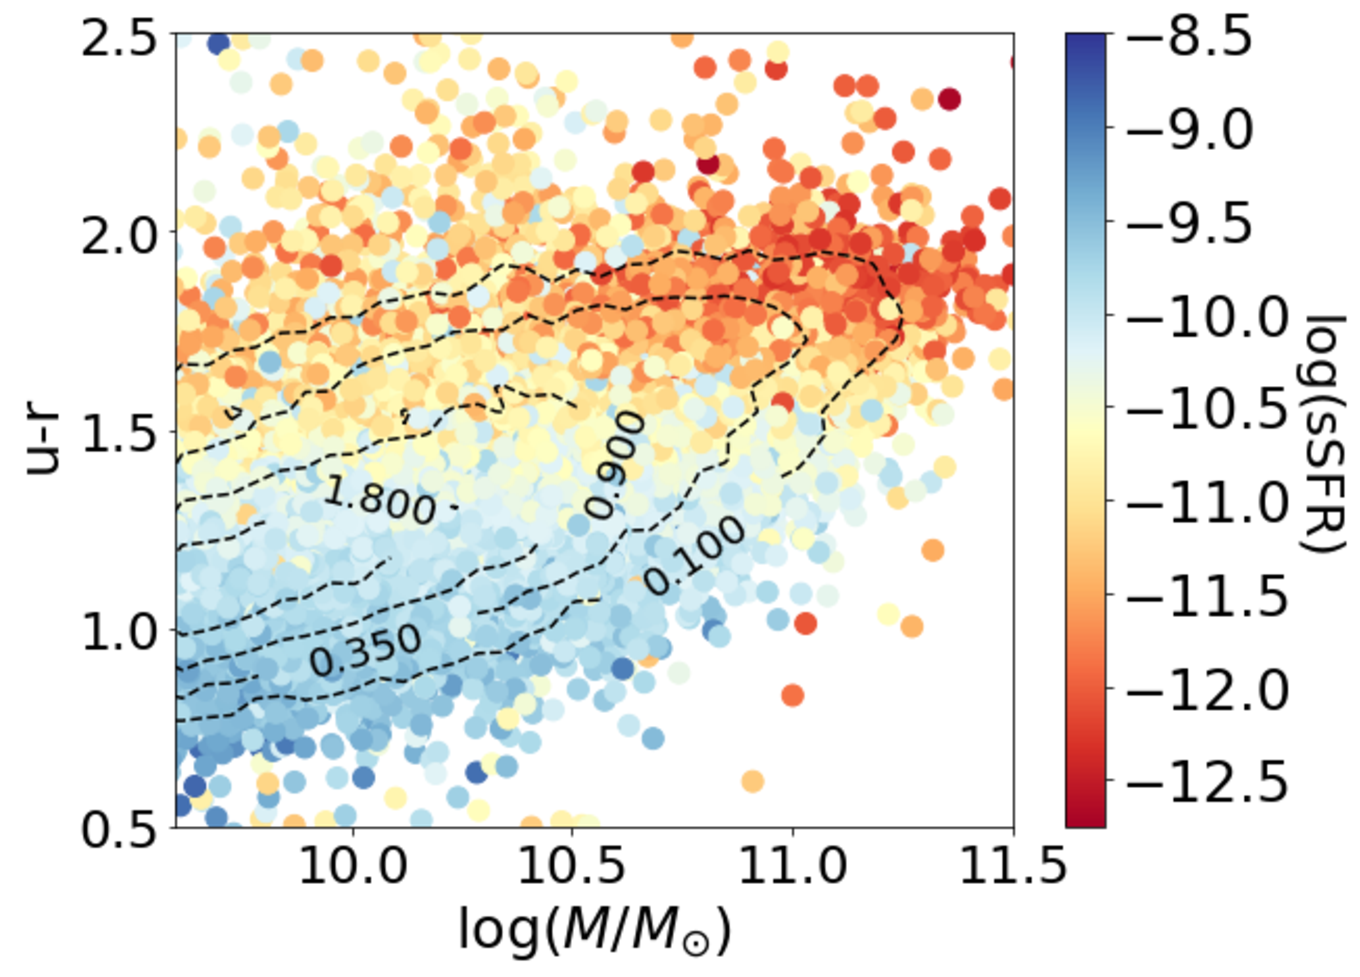
\includegraphics[width=0.47\textwidth]{sdss_disk_scatter.pdf}} &
    \subfigure[Bulge-dominated Galaxies]{\label{fig:sdss_ellips_scatter}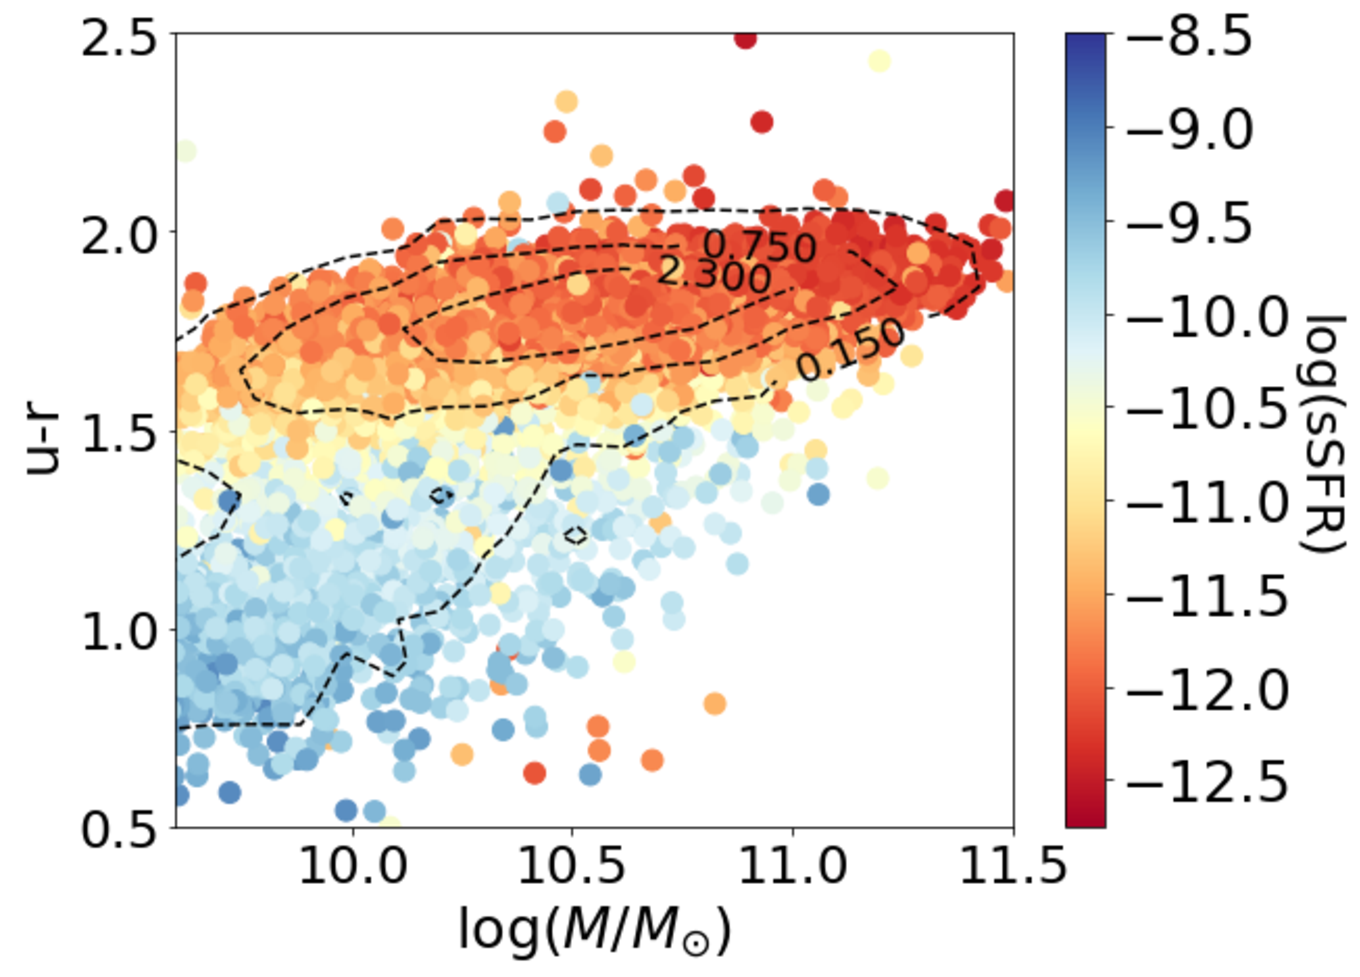
\includegraphics[width=0.47\textwidth]{sdss_ellips_scatter.pdf}} \\
    \subfigure[Disk-dominated Galaxies]{\label{fig:sdss_disk_density}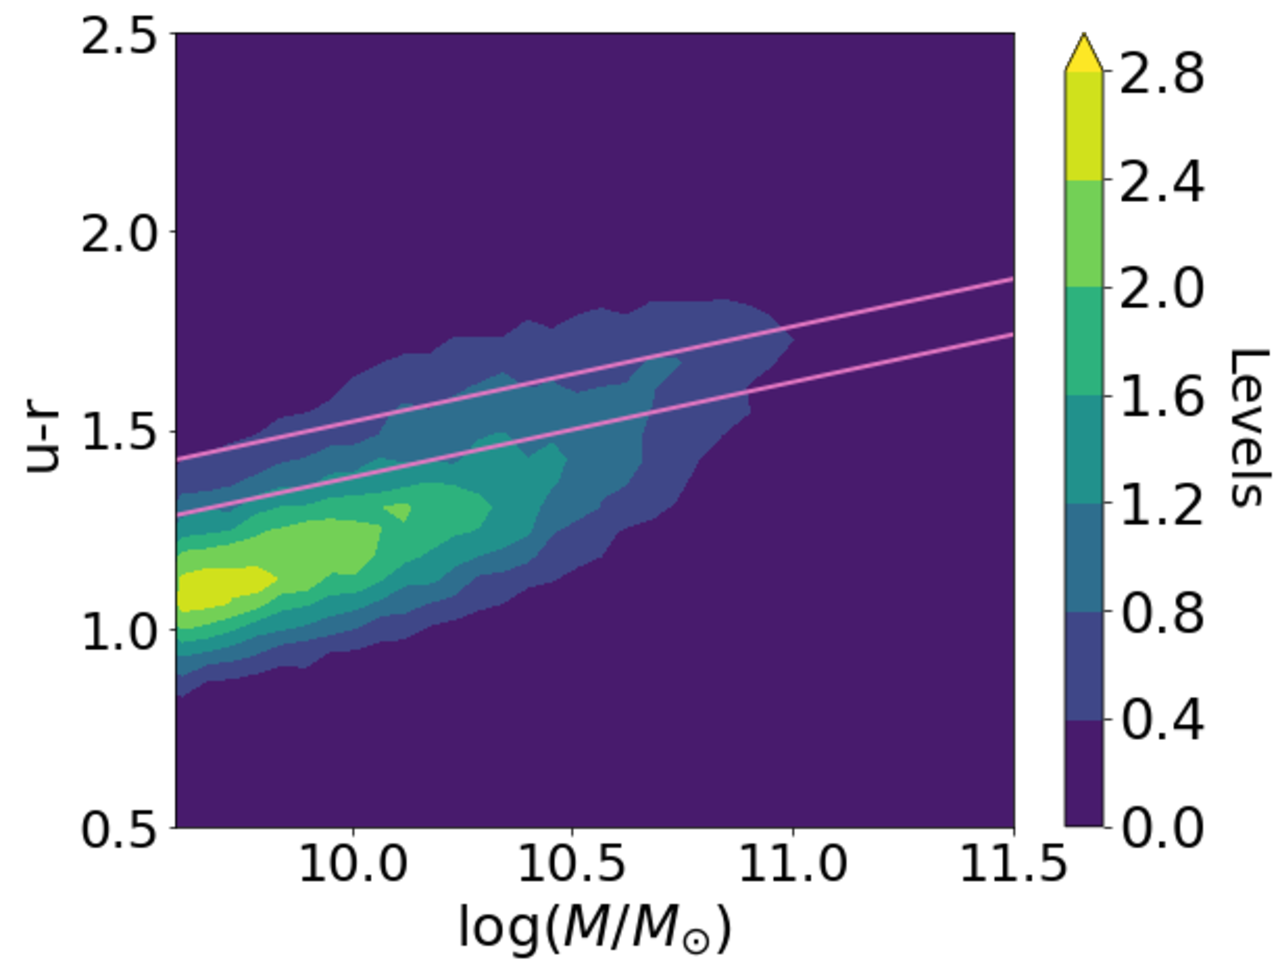
\includegraphics[width=0.47\textwidth]{sdss_disk_density.pdf}} &
    \subfigure[Bulge-dominated Galaxies]{\label{fig:sdss_ellips_density}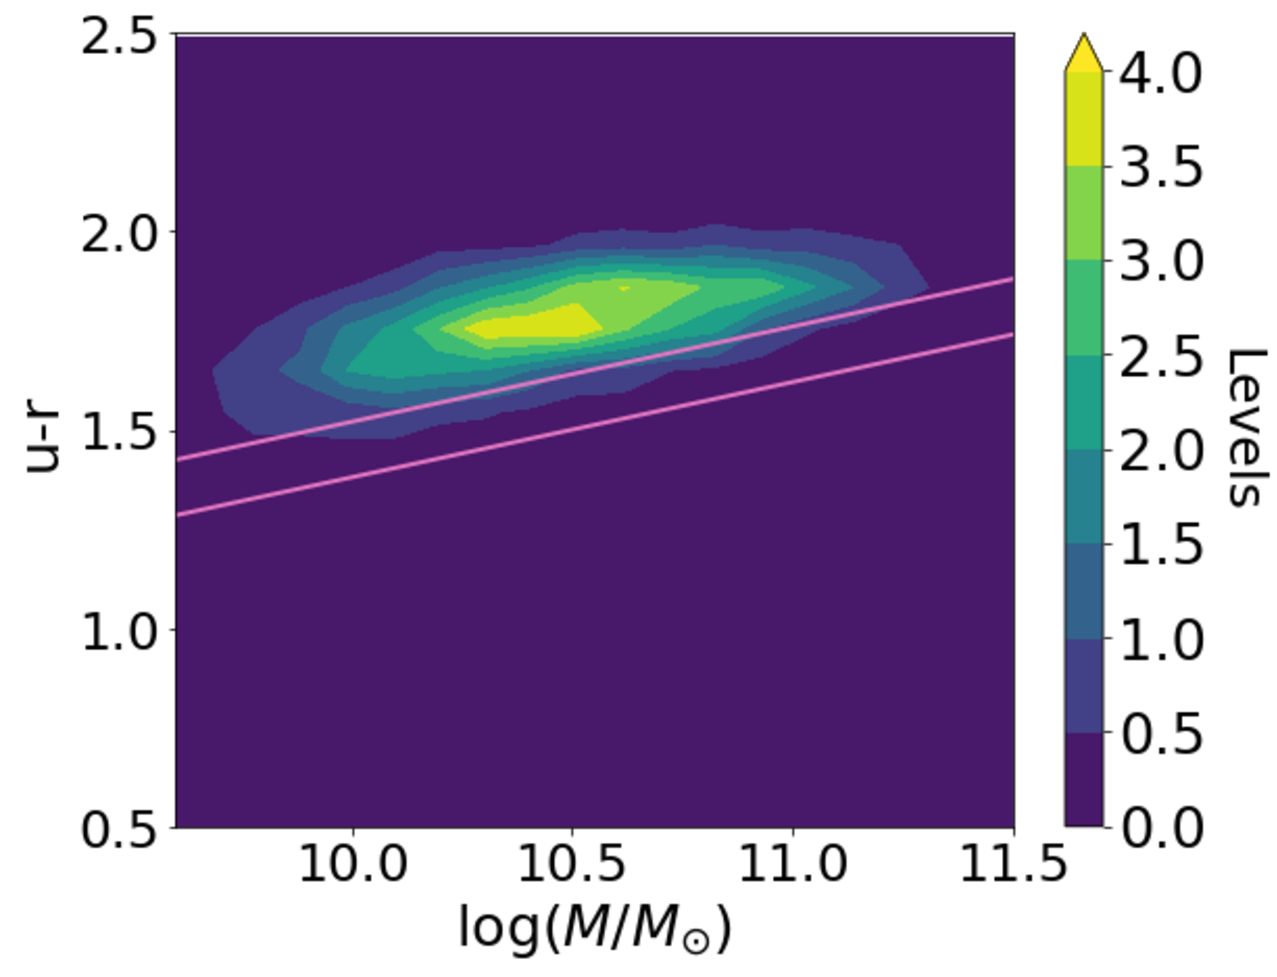
\includegraphics[width=0.47\textwidth]{sdss_ellips_density.pdf}} \\
    \end{tabular}
  \end{center}
  \caption{Color-mass diagrams for the galaxies in the SDSS test set, separated by morphology. Disk-dominated galaxies (panels (a) and (c)) are mostly blue until they reach high masses (and presumably high halo masses), at which point they evolve to the red. In contrast, bulge-dominated galaxies (panels (b) and (d)) are predominately red, and appear to evolve rapidly from a short-lived population of rare, blue ellipticals that likely formed from major mergers of disky star-forming galaxies. Panels (a) and (b) show individual data points, with color indicating the specific star formation rates (sSFR) for each galaxy in units of yr$^{-1}$. Contours show the linear density of galaxies in this plot, and the numbers refer to the levels of the contours. Panels (c) and (d) are the same data plotted in terms of galaxy density. The lines mark the position of the green valley.}
  \label{fig:sdss_cmd}
\end{figure*}


\begin{figure*}[htbp]
	\begin{center}
	\begin{tabular}{ll}
    \subfigure[Disk-dominated Galaxies ]{\label{fig:candels_disk_scatter}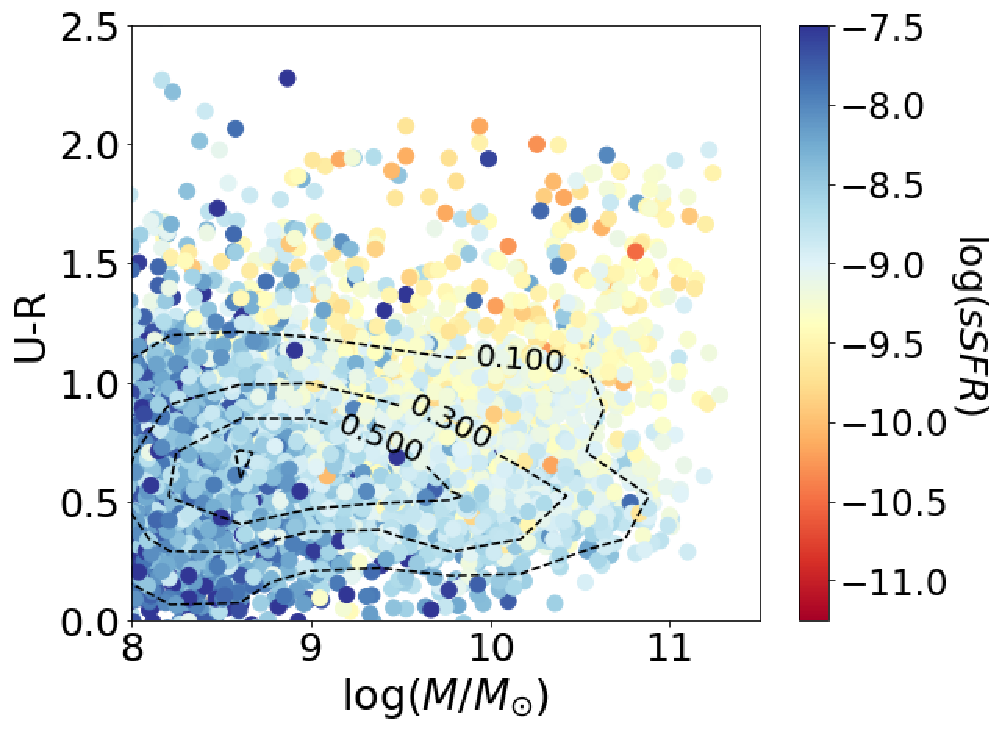
\includegraphics[width=0.47\textwidth]{candels_disk_scatter.pdf}} &
    \subfigure[Bulge-dominated Galaxies ]{\label{fig:candels_ellips_scatter}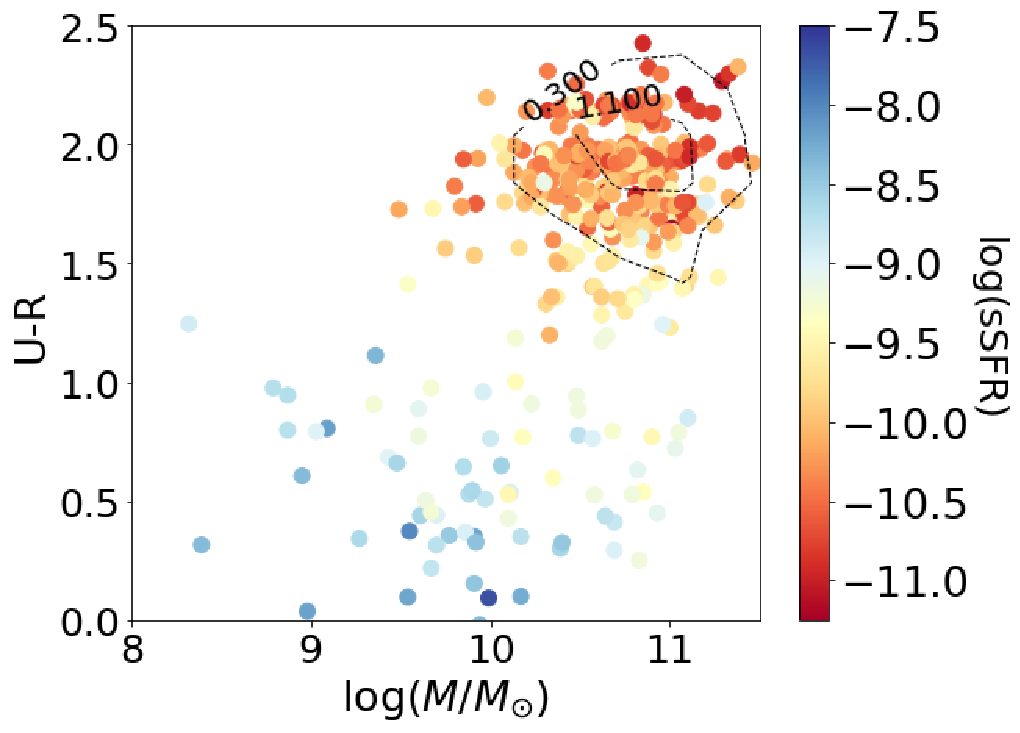
\includegraphics[width=0.47\textwidth]{candels_ellips_scatter.pdf}} \\
    \subfigure[Disk-dominated Galaxies]{\label{fig:candels_disk_density}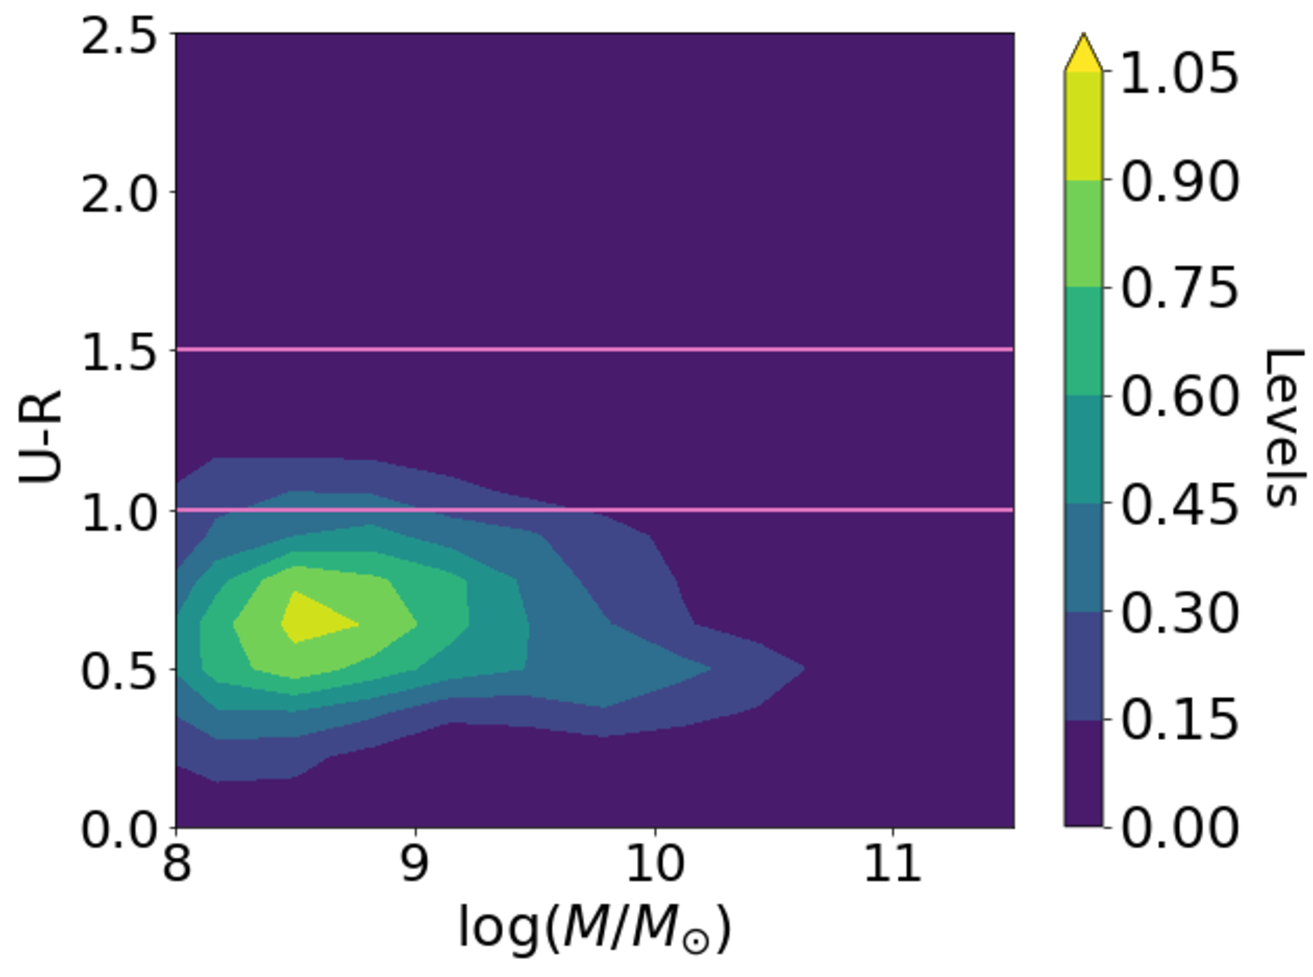
\includegraphics[width=0.47\textwidth]{candels_disk_density.pdf}} &
    \subfigure[Bulge-dominated Galaxies  ]{\label{fig:candels_ellips_density}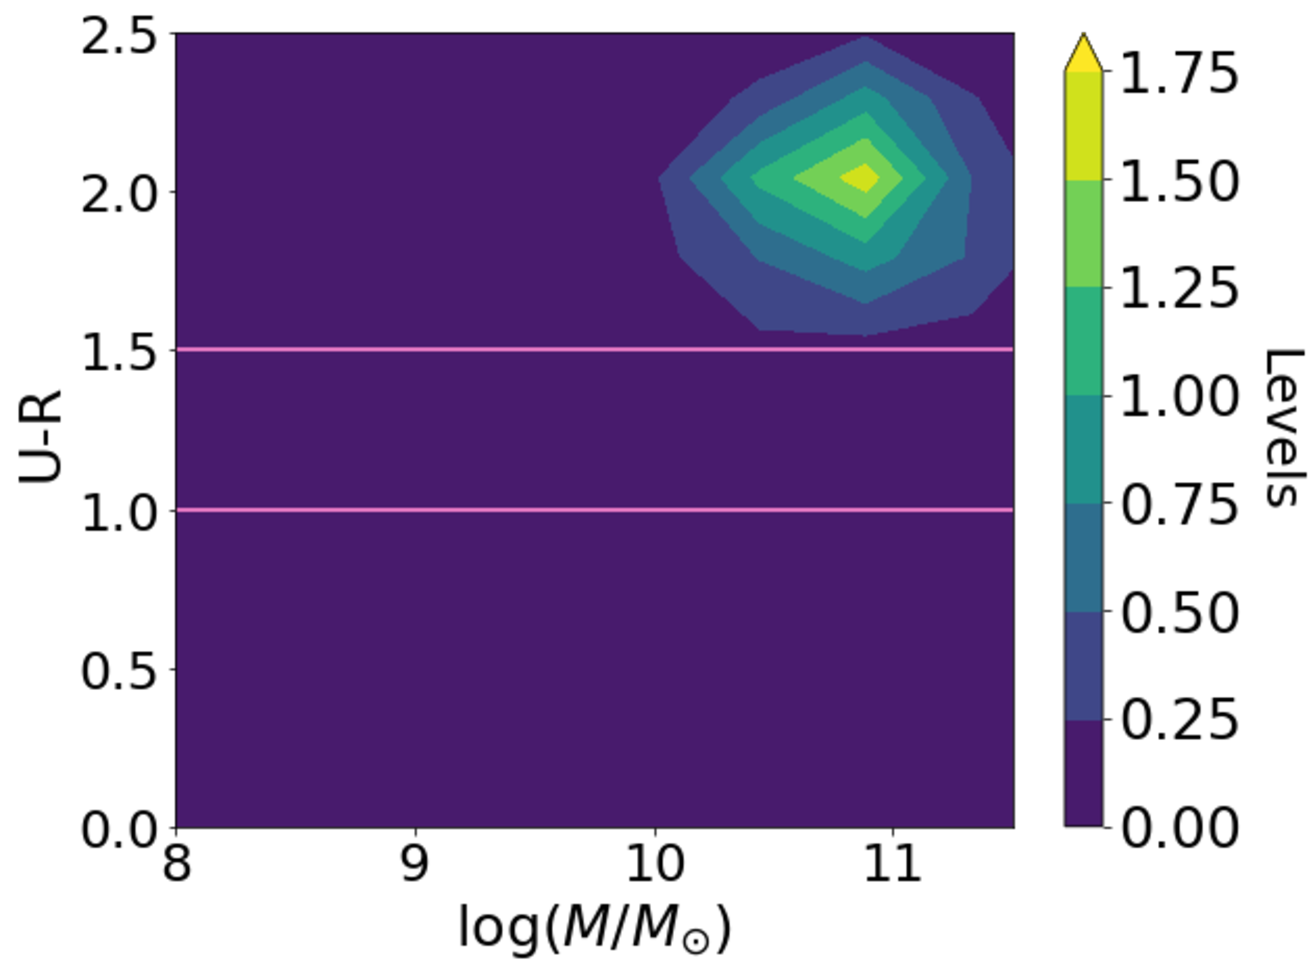
\includegraphics[width=0.47\textwidth]{candels_ellips_density.pdf}} \\
    \end{tabular}
  \end{center}
  \caption{Color-mass diagrams for the galaxies in the CANDELS test set, separated by morphology. Similar to Fig. \ref{fig:sdss_cmd}, disk-dominated galaxies (panels (a) and (c)) show signs of secular evolution, while bulge-dominated galaxies (panels (b) and (d)) appear to evolve rapidly from a short-lived population of rare, blue ellipticals. Panels (a) and (b) show individual data points, with color indicating the specific star formation rates (sSFR) for each galaxy in units of yr$^{-1}$. Contours show the linear density of galaxies in this plot and the numbers refer to the levels of the contours. Panels (c) and (d) are the same data plotted in terms of galaxy density. The lines mark the position of the green valley.}
  \label{fig:candels_cmd}
\end{figure*}

\begin{table}[htbp]
  \centering
  \caption{Statistics of the Color-Mass Diagrams \label{tab:cmd_stats}}
  \begin{tabular}{c|c|cc|cc}
      \hline
      \hline
      \multicolumn{2}{c}{} & \multicolumn{2}{|c|}{SDSS} & \multicolumn{2}{c}{CANDELS}\\ 
      \hline
      \multicolumn{2}{c|}{Galaxy Sample} & Number & Fraction & Number & Fraction\\
      \hline
      \multirow{4}{*}{Disk-dominated} & Blue Cloud & 32870 & 69.16$\%$ & 10614 & 87.10 $\%$ \\ & Green Valley & 7814 & 16.44$\%$ & 1330 & 10.91$\%$ \\ & Red Sequence & 6845 & 14.40$\%$ & 242 & 1.99$\%$ \\ \cline{2-6}
      & Total & 47529 & 100$\%$ & 12186 & 100$\%$ \\ 
      \hline
      \hline
      \multirow{4}{*}{Bulge-dominated} & Blue Cloud & 995 & 12.53$\%$ & 80 & 16.19$\%$ \\ & Green Valley & 633 & 7.97$\%$ & 39 & 7.89$\%$ \\ & Red Sequence & 6313 & 79.50$\%$ & 375 & 75.91$\%$ \\ \cline{2-6}
      & Total & 7941 & 100$\%$ & 494 & 100$\%$ \\
      \hline 
      \multicolumn{6}{p{0.82\textwidth}}{\vskip 0.01cm \small \texttt{NOTE-} The demographics of SDSS and CANDELS galaxies disaggregated by morphology and color. The green valley for both samples is defined in \S\,\ref{sec:cm_results} and the three zones are shown in Figs.\,\ref{fig:sdss_cmd} and \ref{fig:candels_cmd}. We omit galaxies used in training \gamornet{} ($\sim$25\% of each sample) as well as galaxies lacking estimates for the mass or sSFR ($\sim 0.7\%$ for SDSS and $\sim 3.4\%$ for CANDELS).}
  \end{tabular}
  \end{table}

Figure~\ref{fig:sdss_cmd} shows the \textit{u-r} color-mass diagram for the $z \sim 0$ SDSS test set separated by disk- and bulge-dominated morphologies. The color of each point in panels (a) and (b) refer to the specific star formation rate of each galaxy. The contours in all plots refer to the linear number density of galaxies, and the straight lines in panels (c) and (d) mark the location of the green valley, which we define to be the region between the colors mentioned below:

\begin{equation}
    u-r(M) = -1.02 + 0.24\times\log(M/M_{\odot})
\end{equation}

\begin{equation}
    u-r(M) = -0.88 + 0.24\times\log(M/M_{\odot}) .
\end{equation}

\noindent
The \textit{U-R} color-mass diagram for the $z\sim1$ CANDELS data is shown in Figure~\ref{fig:candels_cmd} and this figure is arranged in the same way as Figure~\ref{fig:sdss_cmd}. We define the green valley, in this case, as the region between \textit{U-R} colors $1.0$ and $1.5$. 

The demographics of galaxies by color and morphology for both samples is summarized in Table~\ref{tab:cmd_stats}. Note that the total number of galaxies in the table does not match that in \S\,\ref{sec:morph_results} as we have omitted galaxies that lack estimates of either mass or sSFR. The omitted fraction is $\sim 0.7\%$ and $\sim 3.4\%$ for the SDSS and CANDELS samples, respectively. 

For both the samples, we see that both bulge- and disk-dominated galaxies span the entire range of colors (i.e., we see examples of red disk-dominated galaxies as well blue bulge-dominated galaxies). As expected, the disk-dominated galaxies peak in the blue cloud while the bulge-dominated galaxies dominate the red sequence. The green valley is not a feature for either morphology; that is, there is no bimodality. Rather, the number density of galaxies declines monotonically from a red or blue peak. Thus, the green valley only arises when plotting the color-mass diagram of all galaxies together, as was first pointed out for $z\sim0$ galaxies by \citet{schawinski_14_green_herring}.

Figs.\,\ref{fig:sdss_disk_density} and \ref{fig:candels_disk_density} show that the disk-dominated galaxies peak in the blue cloud and decline gradually to the red sequence, in a unimodal way. This suggests that the disks undergo a gradual decline in star formation as opposed to being rapidly quenched through the green valley into the red sequence. At high masses, there are relatively more red disk-dominated galaxies, suggesting that high halo masses may play a role in shutting off the gas supply and quenching star formation. These conclusions agree with other studies of star formation in local galaxies \citep{tojeiro_13,schawinski_14_green_herring,lopes_16,powell_17}.

Conversely, bulge-dominated galaxies in both samples show a unimodal peak in the red sequence, with very few precursors at green and blue colors. 
This is consistent with a scenario in which bulge-dominated galaxies form from major mergers of disk-dominated blue galaxies and then are rapidly quenched through the green valley \citep{schawinski_14_green_herring}.

The morphology-sorted color-mass diagrams we obtained using \gamornet{} classifications largely agree with the previous results of \citet{schawinski_14_green_herring} at $z\sim0$ and \citet{powell_17} at $z \sim 1$; although, in the latter case, we present an order of magnitude more galaxies. For both samples, the galaxy fractions in the three zones of the color-mass diagram differ at the few percent level with respect to \citet{schawinski_14_green_herring} and \citet{powell_17}. It is important to note here that our definition of the green valley is slightly different from that used by \citet{schawinski_14_green_herring} due to their use of reddening corrected colors. Besides, \cite{schawinski_14_green_herring} and \cite{powell_17} used visual classification and GALFIT, respectively, compared to our use of \gamornet{}. Finally, our sample sizes are much larger: at $z \sim 0$, we have twice as many galaxies as \citet{schawinski_14_green_herring}, and at $z\sim1$, we have six times the galaxies analyzed by \citet{powell_17}. Larger samples are particularly important for bins with low statistics. For example, \cite{powell_17} identified only 5 bulge-dominated galaxies in the green valley, whereas we find 39, so the statistical uncertainties on that fraction are lower.

\begin{figure*}[htb]
	\begin{center}
    \subfigure[$z\sim0$ SDSS sample ]{\label{fig:ssfr_sdss}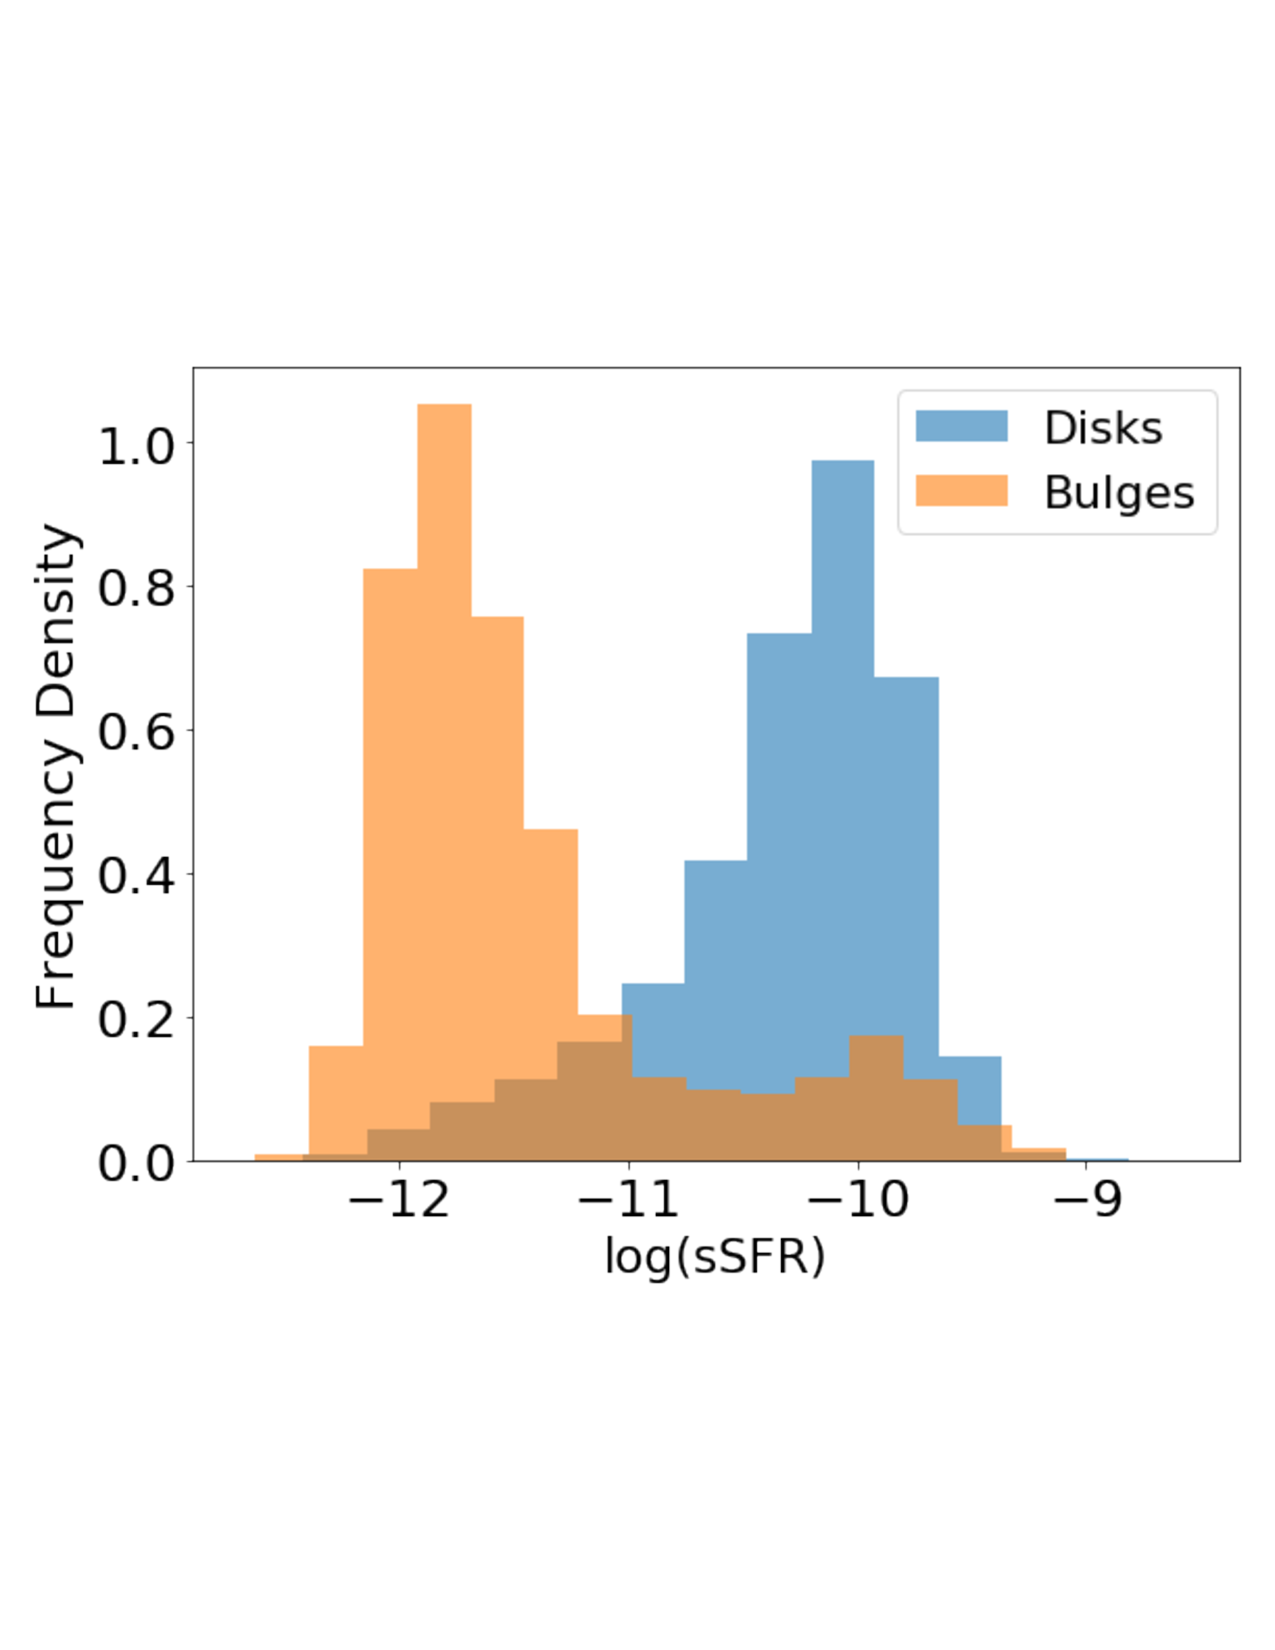
\includegraphics[width=0.47\textwidth]{ssfr_sdss.pdf}}
    \subfigure[$z\sim1$ CANDELS sample]{\label{fig:ssfr_candels}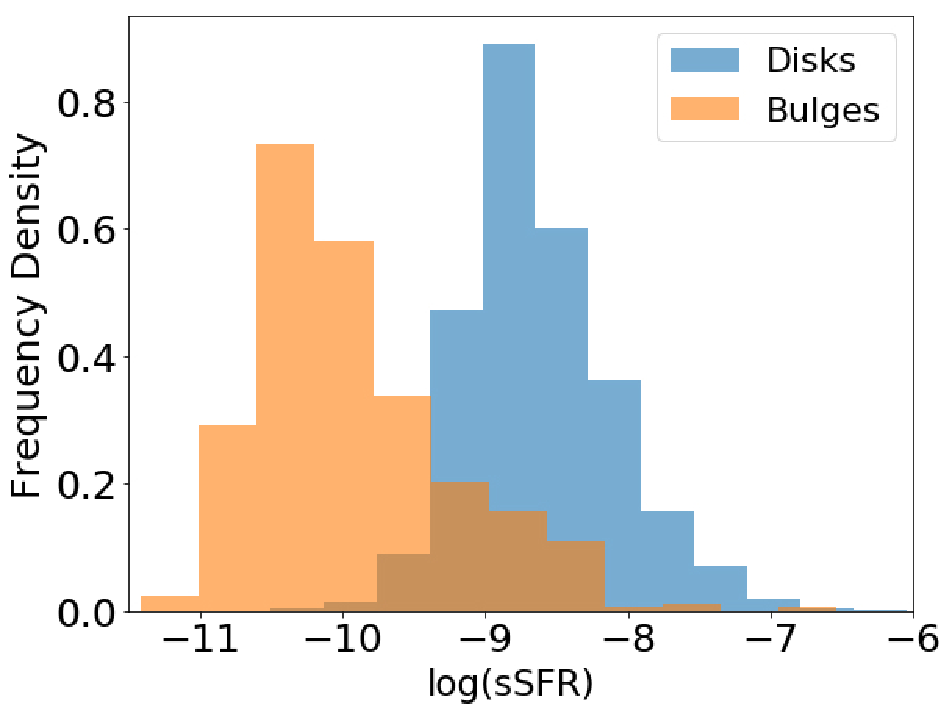
\includegraphics[width=0.48\textwidth]{ssfr_candels.pdf}}
  \end{center}
  \caption{The normalized distribution of the specific star formation rate\,(sSFR), separated by morphology, for the SDSS and CANDELS data sets as obtained from the MPA-JHU and 3D-HST catalogs, respectively. `Frequency density' refers to the number counts normalized to form a probability density.}
  \label{fig:ssfr_distr}
\end{figure*}

Figure~\ref{fig:ssfr_distr} shows the distribution of sSFR separated by morphology. For both samples, the distribution of bulge-dominated galaxies peaks at a lower sSFR, showing the association of disk-dominated galaxies with consistent secular star formation and bulge-dominated galaxies with recent quenching. 

\section{Summary and Discussion} \label{sec:disc}
In this article, we introduced \gamornet{}, a convolutional neural network\,(CNN) that can classify galaxies morphologically. We first trained \gamornet{} on simulations of galaxies with a bulge and a disk component (\S\,\ref{sec:simulation_code}) to separate galaxies according to their bulge-to-total ratio ($L_B/L_T$). To make the network better at handling real galaxies, we then transfer learned (\S\,\ref{sec:tf_intro}) on $\sim25\%$ of both the SDSS $z\sim0$ and CANDELS $z\sim1$ samples and thereafter tested the network on the remaining $\sim75\%$ of both the samples. The net misclassification rate (calculated by weighting the disk- and bulge-dominated accuracies appropriately) achieved for both samples is $\lesssim 5\%$. For the SDSS test set of 82,547 galaxies, we achieved accuracies of $99.7\%$ for disk-dominated galaxies and $94.8\%$ for bulge-dominated galaxies. The corresponding numbers for the CANDELS test set of 21,746 galaxies are $91.8\%$ and $78.6\%$. We showed in \S\,\ref{sec:morph_results} that the misclassified CANDELS galaxies are dominated by galaxies with a half-light radius comparable to the PSF and galaxy images with low S/Ns. 

Although it has previously been shown that CNNs can be used to recover single-component \sersic{} fits of galaxies and visual morphologies \citep[eg.][]{company_15,tuccillo_18}, according to our knowledge, this is the first time it has been demonstrated that CNNs can be used to classify galaxies according to their bulge-to-total ratios.

More importantly, this work demonstrates that \gamornet{} can be applied across different data sets to perform morphological classification without the need for a large training set of real galaxies. By using a roughly 25-75 train-test split during transfer learning, we have clearly demonstrated that even when training on $25\%$ of the total sample, \gamornet{} can generalize beyond the training data and classify galaxies with high accuracy. This has very important consequences, as the applicability of CNNs to future data-intensive surveys like LSST, WFIRST, and Euclid will depend on their ability to perform without the need for a large training set of real data.

We make the source code of \gamornet{}, the trained network models, as well the morphological classifications of all the galaxies in our sample available to the public (Appendix \ref{sec:ap:public_data_release}). Although \gamornet{}-S and -C were tuned for \textit{g}-band and \textit{H}-band images, respectively, the networks should perform with comparable accuracies in other nearby bands for all SDSS $z\sim0$ and CANDELS $z\sim1$ galaxies. We also make available the weights and biases of \gamornet{} before transfer learning, i.e., after training with simulations only, so that additional data sets can be used for transfer learning. Our general prescription of training on simulations and then transfer learning should work for morphological classifications of any data set.

In \S\,\ref{sec:cm_results}, we used the morphological classifications obtained using \gamornet{} (\S\,\ref{sec:morph_results}) to study the quenching of star formation using the color-mass diagrams of our samples at $z\sim0$ and $z\sim1$\,.

For both samples, the morphology-separated color-mass diagrams do not show any bimodality. The disk-dominated galaxies peak in the blue cloud and then gradually extend to the red sequence, suggesting that quenching in disks is a secular process. Conversely, bulge-dominated galaxies in both samples peak  in  the  red  sequence,  with  very few precursors in the green valley and blue cloud. This is consistent with a scenario in which bulge-dominated galaxies form from major mergers of disk-dominated blue galaxies and then are rapidly quenched through the green valley.

Our results largely agree with previous similar studies performed at these redshifts. Our sample sizes are twice and six times as large, respectively, as those in the two previous studies done using visual classifications \citep{schawinski_14_green_herring} and using GALFIT \citep{powell_17}. The reason that we were able to use such large sample sizes is that \gamornet{}, once trained, can process large data sets very quickly and easily compared to more traditional methods.

In the future, we aim to use \gamornet{} to study the correlation of AGN with host galaxy morphology. We also plan to take \gamornet{} beyond bulge/disk classification and use it to derive different properties of AGN host galaxies. 

\section*{Chapter Acknowledgements}
We would like to thank the anonymous referee for a thorough review of the manuscript and suggesting changes that greatly improved the quality and clarity of our manuscript.

This work used data from SDSS. Funding for the SDSS and SDSS-II has been provided by the Alfred P. Sloan Foundation, the Participating Institutions, the National Science Foundation, the U.S. Department of Energy, the National Aeronautics and Space Administration, the Japanese Monbukagakusho, the Max Planck Society, and the Higher Education Funding Council for England. The SDSS website is \href{http://www.sdss.org/}{http://www.sdss.org/}.

The SDSS is managed by the Astrophysical Research Consortium for the Participating Institutions. The Participating Institutions are the American Museum of Natural History, Astrophysical Institute Potsdam, University of Basel, University of Cambridge, Case Western Reserve University, University of Chicago, Drexel University, Fermilab, the Institute for Advanced Study, the Japan Participation Group, Johns Hopkins University, the Joint Institute for Nuclear Astrophysics, the Kavli Institute for Particle Astrophysics and Cosmology, the Korean Scientist Group, the Chinese Academy of Sciences (LAMOST), Los Alamos National Laboratory, the Max-Planck-Institute for Astronomy (MPIA), the Max-Planck-Institute for Astrophysics (MPA), New Mexico State University, Ohio State University, University of Pittsburgh, University of Portsmouth, Princeton University, the United States Naval Observatory, and the University of Washington.

This work is based on observations taken by the CANDELS Multi-Cycle Treasury Program with the NASA/ESA HST, which is operated by the Association of Universities for Research in Astronomy, Inc., under NASA contract NAS5-26555.

This work is based on observations taken by the 3D-HST Treasury Program with the NASA/ESA HST, which is operated by the Association of Universities for Research in Astronomy, Inc., under NASA contract NAS5-26555.

This material is based upon work supported by the National Science Foundation under grant No. 1715512

C.M.U would like to acknowledge support from National Aeronautics and Space Administration via ADAP Grant 80NSSC18K0418. 

\begin{subappendices}
    
\chapter*{Appendix}\label{ch:gamornet_appendix}

\section{Public Release of Code, Models, and Galaxy Morphological Classifications}\label{sec:ap:public_data_release}

Here, we provide an outline of all the material that we make public as a part of this work. An up-to-date record of this public data release will also be maintained at \href{http://gamornet.ghosharitra.com}{http://gamornet.ghosharitra.com} and \href{http://www.astro.yale.edu/aghosh/gamornet.html}{http://www.astro.yale.edu/aghosh/gamornet.html} in case any of the URLs below stop working over time.   

\subsection{\gamornet{} Source Code}\label{sec:ap:gamornet_source_code}

\gamornet{} was implemented using TFLearn\,\,(\href{http://tflearn.org}{http://tflearn.org}), which is a high-level Application Program Interface for TensorFlow\,\,(\href{https://tensorflow.org}{https://tensorflow.org}), an open source library widely used for large-scale machine learning applications.

The source code of \gamornet{} is maintained as a GitHub Repository and is available at \href{https://github.com/aritraghsh09/GaMorNet}{https://github.com/aritra ghsh09/GaMorNet}. Instructions for installing TFLearn and using \gamornet{} are available in the above GitHub repository. An implementation of \gamornet{} in Keras (\href{https://keras.io/}{https://keras.io/}) is also available at the above repository. 

\subsection{\gamornet{} Trained Models }\label{sec:ap:gamornet_trained_models}

Trained Models for both \gamornet{}-S and -C are being made available as a part of this data release. 

For more details about the various stages of training, refer to \S\,\ref{sec:initial_training} \& \ref{sec:tf_intro}. All of the models below are being made available via Yale Astronomy's Public FTP service \href{ftp://ftp.astro.yale.edu/pub/aghosh/gamornet/trained_models}{\url{ftp://ftp.astro.yale.edu/pub/aghosh/gamornet/trained\textunderscore models}}. 

You can copy and paste the above link into a browser window to download the files, or you can also issue the following commands from a terminal to login to the ftp server

\begin{verbatim}
ftp ftp.astro.yale.edu
\end{verbatim}

Use the username `anonymous' and keep the password field blank. After logging-in, do the following:

\begin{verbatim}
cd pub/aghosh/gamornet/<appropriate_subdirectory> 
get <file_name>
quit
\end{verbatim}

To list the files at your current location, you can use the `ls' command. 

The various subdirectories are named as follows in the list below:

\begin{enumerate}
    \item \gamornet{}-S model trained only on simulations $\xrightarrow{}$ \path{/trained_models/SDSS/sim_rained/}
    \item \gamornet{}-S model trained on simulations and transfer learned on real data $\xrightarrow{}$ \path{/trained_models/SDSS/tl/}
    \item \gamornet{}-C model trained only on simulations $\xrightarrow{}$ \path{/trained\_models/CANDELS/sim_trained/}
    \item \gamornet{}-C model trained on simulations and transfer learned on real data $\xrightarrow{}$ \path{/trained_models/CANDELS/tl/}
\end{enumerate}

Models 2 and 4 can be applied directly to SDSS \textit{g}-band data at $z\sim0$ and CANDELS \textit{H}-band data at $z\sim1$ (or data in other nearby bands), respectively, without any further training. However, if you plan to apply \gamornet{} to data that is different from the above mentioned data sets, we recommend using any of the models above and then transfer learning on your new data. The exact nature of the data will decide which of the models above is the best starting point for the transfer learning process. 

For more information on how to load these models in TFLearn and use them, refer to the documentation of the \gamornet{} GitHub repository mentioned in Sec.~\ref{sec:ap:gamornet_source_code}.

\subsection{ Tables with predicted probabilities and classifications}\label{sec:ap:prob_tables}
                                                                          
The predicted probabilities (of being disk-dominated, bulge-dominated, or indeterminate) and the final classifications for all the galaxies in our SDSS and CANDELS test sets, as determined by \gamornet{}-S and -C, are made available below as .txt files. These tables are the full versions of Tables~\ref{tab:lt_sdss} \&~\ref{tab:lt_candels}.

Both the tables are being made available via Yale Astronomy's Public FTP service \href{ftp://ftp.astro.yale.edu/pub/aghosh/gamornet/pred_tables}{\url{ftp://ftp.astro.yale.edu/ pub/aghosh/gamornet/pred\_tables}}. Instructions for accessing the service from the command line can be found in \S\,\ref{sec:ap:gamornet_trained_models}. The two files are located according to the list below:

\begin{itemize}
    \item Full version of Table~\ref{tab:lt_sdss} corresponding to the SDSS data set $\xrightarrow{}$ \path{/pred_tables/pred_table_sdss.txt}
    \item Full version of Table~\ref{tab:lt_candels} corresponding to the CANDELS data set $\xrightarrow{}$ \path{/pred_tables/pred_table_candels.txt}
\end{itemize}

\subsection{ GalaxySim Source Code }\label{sec:ap:galsim}

The code that was used to simulate the galaxies described in \S\,.\ref{sec:simulation_code} is available as a GitHub repository at \href{https://github.com/aritraghsh09/GalaxySim}{https://git hub.com/aritraghsh09/GalaxySim}

This code makes use of GALFIT\,\citep{galfit} to simulate idealized double component galaxies. Since the simulations of galaxy surface brightness profiles are independent of each other, the code could be trivially parallelized. Instructions for using GalaxySim are available in the above GitHub repository. 

\end{subappendices}
\chapter{GaMPEN: A Machine Learning Framework for Estimating Bayesian Posteriors of Galaxy Morphological Parameters}

Originally published by the American Astronomical Society in \textit{The Astrophysical Journal}, Volume 935, Issue 2, pp. 138, DOI:\href{https://iopscience.iop.org/article/10.3847/1538-4357/ac7f9e}{10.3847/1538-4357/ac7f9e}\\
{\large \emph{Aritra Ghosh, C. Megan Urry, Amrit Rau, Laurence Perreault-Levasseur, Miles Cranmer, Kevin Schawinski, Dominic Stark, Chuan Tian, Ryan Ofman, Tonima Tasnim Ananna, Connor Auge, Nico Cappelluti, David B. Sanders, and Ezequiel Treister} }\\


We introduce a novel machine learning framework for estimating the Bayesian posteriors of morphological parameters for arbitrarily large numbers of galaxies.
The Galaxy Morphology Posterior Estimation Network (\gampen{}) 
estimates values and uncertainties for a galaxy's bulge-to-total light ratio ($L_B/L_T$), effective radius ($R_e$), and flux ($F$). To estimate posteriors, \gampen{} uses the Monte Carlo Dropout technique and incorporates the full covariance matrix between the output parameters in its loss function. %The latter accounts for covariances among the output parameters, and thus the predicted posteriors can be calibrated properly.  
\gampen{} also uses a Spatial Transformer Network (STN) to automatically crop input galaxy frames to an optimal size before determining their morphology. This will allow it to be applied to new data without prior knowledge of galaxy size.
Training and testing \gampen{} on galaxies simulated to match $z < 0.25$ galaxies in Hyper Suprime-Cam Wide \textit{g}-band images, we demonstrate that \gampen{} achieves typical errors of $0.1$ in $L_B/L_T$, $0.17$ arcsec ($\sim 7\%$) in $R_e$, and $6.3\times10^4$ nJy ($\sim 1\%$) in $F$. \gampen{}'s predicted uncertainties
are well-calibrated and accurate ($<5\%$ deviation) -- for regions of the parameter space with high residuals, \gampen{} correctly predicts correspondingly large uncertainties.
%Testing shows that \gampen{} predictions become less precise for especially small ($R_e < 1\arcsec$) and/or faint ($F < 10^6$ nJy) galaxies,where \gampen{} correctly predicts correspondingly larger uncertainties.
We also demonstrate that we can apply categorical labels (i.e., classifications such as ``highly bulge-dominated") to predictions in regions with high residuals and verify that those labels are  $\gtrsim 97\%$ accurate. To the best of our knowledge, \gampen{} is the first machine learning framework for determining joint posterior distributions of multiple morphological parameters and is also the first application of an STN to optical imaging in astronomy.


\section{Introduction} \label{sec_c2:intro}
For almost a century, starting with \citeauthor{hubble_1926} in \citeyear{hubble_1926}, astronomers have linked the morphology of galaxies to the physics of  galaxy formation and evolution. Morphology has been shown to be related to many fundamental properties of the galaxy and its environment, including galaxy mass, star formation rate, stellar kinematics, merger history, cosmic environment, the influence of supermassive black holes \citep[e.g.,][]{Bender1992DynamicallyProperties,Tremaine2002TheCorrelation,pozzetti_10, wuyts_11, Schawinski2014TheGalaxies, Huertas-Company2016MassCANDELS,powell_17, Shimakawa2021Subaru0.30.6, Dimauro2022CoincidenceGrowth}. Studying the morphology of large samples of galaxies at different redshifts is crucial in order to understand the physics of galaxy formation and evolution. 

Over the last decade, machine learning (ML) has been increasingly employed by astronomers for a wide variety of tasks -- from identifying exoplanets to studying black holes \citep[e.g.,][]{ml_pz,ml_sz,Shallue2018IdentifyingKepler-90,Sharma2020ApplicationClassification,Natarajan2021QuasarNet:Holes}. Especially, Convolutional Neural Networks (CNNs)\footnote{CNNs are a specific form of machine learning algorithm that specializes in processing data with a grid-like topology, such as an image. See \S \ref{sec_c2:cnn_description} for more details.} have revolutionized the field of image processing and have become increasingly popular for determining galaxy morphology \citep[e.g.,][]{Dieleman2015Rotation-invariantPrediction, Huertas-Company2015ALEARNING, Tuccillo2018DeepFitting, Hausen2020MorpheusData, Walmsley2020GalaxyLearning, Cheng2021GalaxyNetworks, Vega-Ferrero2021PushingSurvey, Tarsitano2022ImageLearning}. Previously, we have developed a publicly available CNN, called \gamornet{} \citep{Ghosh2020GalaxyGalaxies}, that classifies galaxies morphologically with minimal real training data, and has been demonstrated to achieve accuracy $\gtrsim 95\%$ across multiple datasets. 

This use of CNNs has been driven by the fact that traditional methods of classifying morphologies---visual classification and template fitting to the surface brightness profile of a galaxy---are not scalable to the data volume expected from future surveys such as The Vera Rubin Observatory Legacy Survey of Space and Time \citep[LSST;][]{lsst}, the Nancy Grace Roman Space Telescope \citep[NGRST;][]{ngrst}, and Euclid \citep{euclid}. The quality of fits obtained using template fitting depends significantly on the initial input parameters, and when dealing with millions of galaxies, such hand-refinement of input parameters is an intractable task. Although large citizen science projects like Galaxy Zoo \citep{gzoo_original} have been successful in processing many surveys in the past, even these will fail to keep up with the upcoming data glut. Moreover, reliable visual classifications require a decent signal-to-noise ratio, take time to set up and execute, and require an extremely careful de-biasing of the vote shares obtained \citep[e.g.,][]{gzoo_original,gzoo_candels}. 

From early attempts at using a CNN to classify galaxies morphologically (e.g.,  \citealp{Dieleman2015Rotation-invariantPrediction}) to the largest CNN produced morphology catalogs currently available \citep{Cheng2021GalaxyNetworks, Vega-Ferrero2021PushingSurvey}, most
CNNs have provided broad, qualitative classifications, rather than 
numerical estimates of morphological parameters. Such studies typically entail classifying galaxies based on their morphological properties (e.g., based on whether the galaxy has a disk or a bulge or a bar, etc.) as opposed to predicting values of relevant morphological parameters that help characterize the galaxy (such as bulge-to-total light ratio, radius, etc.).
By contrast, \citet{Tuccillo2018DeepFitting} used a CNN to estimate the parameters of a single-component \sersic{} fit, though  without uncertainties. 
Meanwhile, the computation of full Bayesian posteriors for different morphological parameters is crucial for drawing scientific inferences that account for uncertainty and thus are indispensable in 
the derivation of robust scaling relations  \citep[e.g.,][]{Bernardi2013TheProfile, vanderWel20143D-HST+CANDELS:3} or tests of theoretical models using morphology \citep[e.g.,][]{Schawinski2014TheGalaxies}. Thus, producing posterior estimates will significantly increase the scientific potential of morphological catalogs produced using CNNs.

In this work, we introduce \gampen{} (the Galaxy Morphology Posterior Estimation Network), a novel machine learning framework that estimates the Bayesian posteriors for three morphological parameters: the bulge-to-total light ratio ($L_B/L_T$), the effective radius ($R_e$), and the total flux ($F$).
\gampen{} uses a %downstream 
CNN module to estimate the joint posterior probability distributions of these parameters. This is done by using the negative log-likelihood of the output parameters as the loss function combined with the Monte Carlo Dropout technique \citep{gal_2016}. We also used the full covariance matrix in the loss function, using a series of algebraic manipulations (see \S \ref{sec_c2:uncertainties}). The full covariance matrix accounts for dependencies among different output parameters and ensures that the posterior distributions for all three output variables are well calibrated.

Although the use of CNNs in the recent past has allowed astronomers to process large data volumes quickly, some challenges related to data pre-processing have remained. One of these challenges has to do with making cutouts of proper sizes. Most trained CNNs require input images of a fixed size---thus, most previous work (e.g., \citealp{Cheng2021GalaxyNetworks, Vega-Ferrero2021PushingSurvey}) has resorted to selecting a large cutout size for which ``most galaxies" would remain in the frame. However, this means that for many galaxies in the dataset, especially smaller ones, typical cutouts contain other galaxies in the frame, often leading to less accurate results. This problem is aggravated when designing a CNN applicable over an extensive range in redshift, which corresponds to a large range of galaxy sizes. Lastly, most previous work has used computations of $R_e$ from previous catalogs to estimate the correct cutout size to choose. This is, of course, not possible when one is trying to use a CNN on a new, unlabeled dataset. 

To address these challenges, \gampen{} automatically crops the input image frames using a Spatial Transformer Network (STN) module upstream of the CNN. STNs are self-consistent modules that can be used for the spatial manipulation of data within machine learning frameworks. In \gampen{}, based on the input image, the STN predicts the parameters of an affine transformation which is then applied to the input image. The transformed image is then passed onto the downstream CNN.
The inclusion of the STN in the framework greatly reduces the amount of time spent on data pre-processing as it trains simultaneously with the downstream CNN without additional supervision. We later show in \S \ref{subsec_c2:STN} how the STN automatically learns to make appropriate affine transformations (such as cropping) on the input data, which are helpful in the downstream task of morphological parameter estimation.

To the best of our knowledge, \gampen{} is the first ML framework to apply an STN to optical imaging data and is the first to estimate full Bayesian posteriors for galaxy morphological parameters. In order to have a robust understanding of the performance, bias, and limitations of \gampen{}, we train and test \gampen{} on simulations of galaxy images---the only situation where we have access to the ``ground truth" morphological parameters of the galaxies. We match our simulations to the observations of the Hyper Suprime-Cam (HSC) Wide survey \citep{hsc_pdr1}, as this is an obvious application (to be described in a forthcoming paper).
%In a future paper, we will describe the application of \gampen{} to real HSC data. 
We use real HSC Wide images, with their multiples galaxies, to validate the STN performance.


In \S \ref{sec_c2:sim_data}, we describe the simulated data used to train and test \gampen{}. We describe the structure and code of \gampen{} in \S \ref{sec_c2:cnn_description} and outline the entire mechanism behind the prediction of posteriors in \S \ref{sec_c2:uncertainties}. In \S \ref{sec_c2:training} we describe \gampen{}'s training procedure. We present our results in \S \ref{sec_c2:results}, and summarize our findings along with future applications of \gampen{} in \S \ref{sec_c2:conclusions}. \gampen{}'s data-access policies are described in Appendix  \ref{sec_c2:ap:data_access}. 

\section{Simulated Galaxies} \label{sec_c2:sim_data}
We train and test \gampen{} using mock galaxy image cutouts simulated to match \textit{g}-band data from the Hyper Suprime-Cam (HSC) Subaru Strategic Program wide-field optical survey \citep{hsc_pdr1}. The Subaru Strategic Program, ongoing since 2014, uses the HSC prime-focus camera, which provides extremely high sensitivity and resolving power due to the large 8.2 meter mirror of the Subaru Telescope. Its \textit{g}-band seeing, with median FWHM of $0.85''$, is a large improvement over the Sloan Digital Sky Survey (SDSS; \citealp{sdss_tech_summary}), which has a median \textit{g}-band seeing of $1.4''$.

To generate mock images, we used GalSim \citep{Rowe2015GalSim:Toolkit}, the modular galaxy image simulation toolkit. GalSim has been extensively tested and shown to yield very accurate rendered images of galaxies. We simulated 150,000 galaxies in total, with a mixture of both single and double components, in order to have a diverse training sample. To be exact, $75\%$ of the simulated galaxies consisted of both bulge and disk components, while the remaining $25\%$ had either a single disk or a bulge. 

For both the bulge and disk components, we used the \sersic{} profile, the surface brightness of which is given by  

\begin{equation}
\Sigma(R) = \Sigma_e \exp \left[ -\kappa \left( \left( \frac{R}{R_e}\right)^{1/n} - 1 \right) \right] ,
\label{eq:sersic_fn}
\end{equation}

\noindent
where $\Sigma_e$ is the pixel surface brightness at the effective radius $R_e$, $n$ is the Se\'rsic index, which controls the concentration of the light profile, and $\kappa$ is a parameter coupled to $n$ that ensures that half of the total flux is enclosed within $R_e$.
The standard formula for an exponential disk corresponds to $n=1$, and a de\,Vaucouleurs profiles is $n=4$.

\begin{table}[htbp]
    \centering
    \caption{Parameter Ranges of Simulated Galaxies  \label{tab_c2:sim_para}}
    \begin{tabular}{cccccc}
    \hline
    \hline
    Component & \sersic{} & Half-Light & Flux & Axis & Position \\ 
    Name &  Index & Radius & & Ratio & Angle \\
     &  & (arcsec) & (nJy) &  & (degrees) \\
     \hline 
     \hline
     \multicolumn{6}{c}{Single Component Galaxies} \\
     \hline
      & 0.8 - 1.2 or 3.5 - 5.0\textsuperscript{a} & 0.1 - 5.0 & $10^3$ - $5\times10^6$ & 0.25 - 1.0 & $-90.0$ - $90.0$ \\
     \hline
     \hline
     \multicolumn{6}{c}{Double Component Galaxies} \\
     \hline
     Disk & 0.8 - 1.2 & 0.1 - 5.0 & 0.0 - 1.0\textsuperscript{b} & 0.25 - 1.0 & $-90.0$ - 90.0\\
     %\hline
     Bulge & 3.5 - 5.0 & 0.1 - 3.0 & 1.0 - Disk \textsuperscript{b} & 0.25 - 1.0 &  Disk $\pm\,[0,15]$\textsuperscript{c} \\ 
     \hline
     \multicolumn{6}{p{0.95\textwidth}}{\vskip 0.01cm \small \textsuperscript{a} The single component galaxies are equally divided between galaxies with a \sersic{} index between 0.8 - 1.2 and galaxies with a \sersic{} index between 3.5 - 5.0.} \\
     \multicolumn{6}{p{0.95\textwidth}}{\textsuperscript{b} Fractional fluxes are noted here. The bulge flux fraction is chosen such that for each simulated galaxy it is added with the disk flux fraction to give $1.0$. The total flux of the galaxies is varied between $10^3$ and $5\times10^6$ nJy.} \\
     \multicolumn{6}{p{0.95\textwidth}}{\textsuperscript{c} The bulge position angle differs from the disk position angle by a randomly chosen value between $-15$ and $+15$ degrees.} \\
     \multicolumn{6}{p{0.95\textwidth}}{\texttt{NOTE-} The above table shows the ranges of the various \sersic{} profile parameters used to simulate training and testing data. $75\%$ of the simulated galaxies have both disk and bulge components, and the remainder have either a disk or a bulge component. The distributions of all the simulation parameters are uniform except for the position angle and flux of the double-component galaxies. For more details about these choices, please refer to  \S\,\ref{sec_c2:sim_data}.} \\
    \end{tabular}
\end{table}

The parameters required to generate the \sersic{} profiles were drawn from uniform distributions, over ranges given in Table \ref{tab_c2:sim_para}. For the disk and bulge components, we let the \sersic{} index vary between $0.8-1.2$ and $3.5-5.0$, respectively. We chose to have varying \sersic{} indices as opposed to fixed values for each component in order to have a training set with diverse light profiles. The parameter ranges for fluxes and half-light radii are quite expansive, such that the simulations represent most local galaxies \citep{binney_and_merrifield} at $z \leq 0.25$ (i.e., the simulation parameters are chosen to match HSC $z < 0.25$ galaxies).

Specifically, single-component galaxies were assigned a half-light radius between $0.25$ kpc and $11.5$ kpc. In the double-component galaxies, the disk half-light radius was varied across the same range, and the bulge half-light radius was varied between $0.25$ kpc and $7.0$ kpc. To obtain the corresponding angular sizes for simulation, we placed the sample at $ z = 0.125$ using the Planck18 cosmology ($H_0=67.7$ km/s/Mpc, \citealp{planck18}) and the appropriate pixel scale.

For the single-component galaxies, the total flux was varied between $10^3$ and $5\times10^6$ nJy ($m_{\mathrm{AB}}\sim14 - 23$). For the double component galaxies, we first draw $L_B/L_T$ from a uniform distribution between 0 and 1. Thereafter, the total flux of the galaxy is chosen from a uniform distribution with a range of $10^3 - 5\times10^6$ nJy. To assign fluxes to the bulge and disk components, we multiply $L_B/L_T$ and $(1 - L_B/L_T)$ respectively by the total flux. Not following this procedure and drawing the bulge and disk fluxes independently causes most galaxies in the training set to have a very high or a very low $L_B/L_T$, which is not the case for most galaxies, and in any case we already have single-component galaxies in our sample. For the double component sample, we wanted to have a sufficient number of galaxies with intermediate values of $L_B/L_T$.

What matters in training a CNN is not matching the observed distributions of the simulation parameters; rather, it is spanning the full range of those parameters. 
Having too many of any one type---even if that is the reality in real data---can result in lower accuracy for minority populations (e.g., \citealp{Ghosh2020GalaxyGalaxies}).
By not weighting the simulated galaxy sample in any specific regions of the parameter space, we are able to optimize \gampen{} for the full range of galaxy morophologies.
%a diverse set of galaxies and are also able to thoroughly investigate whether \gampen{} performs poorly in any specific regions of the parameter space.

\begin{figure}[htb]
    \centering
    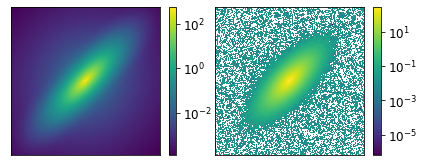
\includegraphics[width = 0.47\textwidth]{sim_process.png}
    \caption{Two stages of simulating an HSC galaxy. (\textit{Left}): A randomly chosen two-dimensional light profile generated by GalSim. (\textit{Right}): The same image after PSF convolution and noise addition. The white pixels represent (small) negative values that arise from the process of noise addition.}
    \label{fig_c2:sim_process}
\end{figure}

To make the two-dimensional light profiles generated by GalSim realistic, we convolved these with a representative point-spread function (PSF), and added appropriate noise. Figure \ref{fig_c2:sim_process} shows a randomly chosen simulated light profile, as well as the corresponding image cutout generated after PSF convolution and noise addition. 

To curate a collection of representative PSFs, we first selected 100 galaxies at random from the HSC PDR2 Wide field \citep{hsc_pdr3} with $z \leq 0.25$ and $m_g \leq 23$, and that did not have any quality flags set to True (the quality flags check for cosmic ray hits, interpolated pixels etc.). We then used the HSC PSF Picker Tool\footnote{\href{https://hsc-release.mtk.nao.ac.jp/psf/pdr3/}{https://hsc-release.mtk.nao.ac.jp/psf/pdr3/}} to obtain the PSF at the location of these 100 galaxies. Each simulated light profile was convolved with a randomly chosen PSF out of these 100. To make sure that the PSFs are representative (i.e., do not contain any outliers), we ran a test where we convolved each one with a simulated galaxy light profile, before adding noise. 
We then inspected all possible difference images for each convolved galaxy, to make sure the average pixel value of the difference image was always at least three orders of magnitude lower than the average pixel value of the convolved galaxy image.

To generate representative noise, we used one-thousand $2\times2$ arcsec ``sky objects" from the HSC PDR2 Wide field. Sky-objects are empty regions identified by the HSC pipeline that are outside object footprints and are recommended for being used in blank-sky measurements. We visually verified that our sky objects did not contain any sources. We then read in the pixel values of these sky objects to generate a large sample of noise pixels. We randomly sampled this collection of noise pixels to make two-dimensional arrays of the same size as that of the simulated images and then added them to the images.

\begin{figure*}[htb]
    \centering
    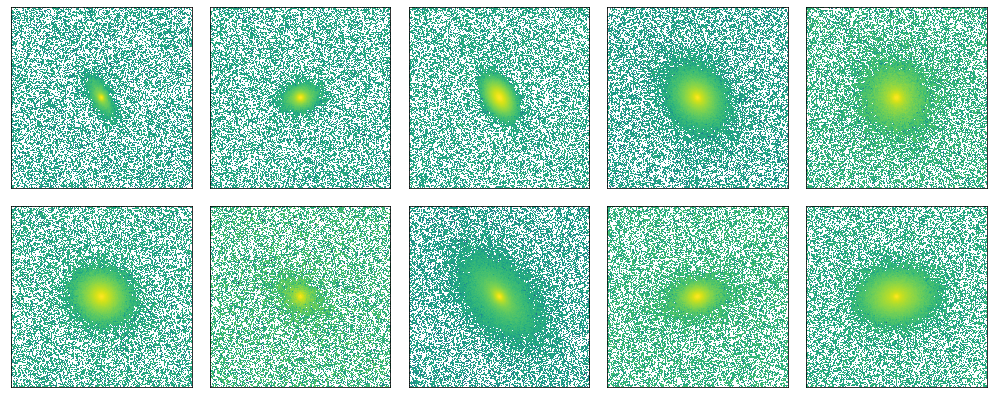
\includegraphics[width
    =\textwidth]{random_sim_galaxies.png}
    \caption{Ten randomly selected galaxies from our simulated dataset. The simulation parameters are chosen such that the simulated galaxies represent a diverse range of light profiles and include most bright, local galaxies at $z \lesssim 0.25$.}
    \label{fig_c2:random_sim_galaxies}
\end{figure*}

All the simulated galaxy cutouts were chosen to have a size of $239 \times 239$ pixels, which translates to roughly $40 \times 40$ arcsecs given HSC's pixel scale of $0.168$ arcsecs/pixel. Ten randomly chosen simulated galaxies from our dataset are shown in Figure \ref{fig_c2:random_sim_galaxies}. 


\section{\gampen{} Architecture} \label{sec_c2:cnn_description}

Artificial neural networks, consisting of many connected individual units called artificial neurons, have been studied for more than five decades. These artificial neurons are usually arranged in multiple layers and such networks typically have (a) an input layer to feed data into the network; (b) an output layer that contains the result of propagating the data through the network. In between, there are additional hidden layer(s). Each neuron is characterized by a weight vector $\bm{w}=(w_1,w_2,\ldots,w_n)$ and a bias $b$. The output of a single neuron in the network is given by 

\begin{equation}
y = \sigma(\bm{w} \cdot \bm{x} + b) ,
\label{eq:neuron_output}
\end{equation}

\noindent
where $\sigma$ is the chosen activation function of the neuron and $\bm{x}$ is the vector of inputs to the neuron. 
The process of training an artificial neural network involves finding the optimum set of weights and biases of all neurons such that, for a given set of inputs, the output of the network resembles the desired outputs as closely as possible. The optimization is usually performed by minimizing a loss function using stochastic gradient descent.

%\begin{figure}[htb]
%    \centering
%    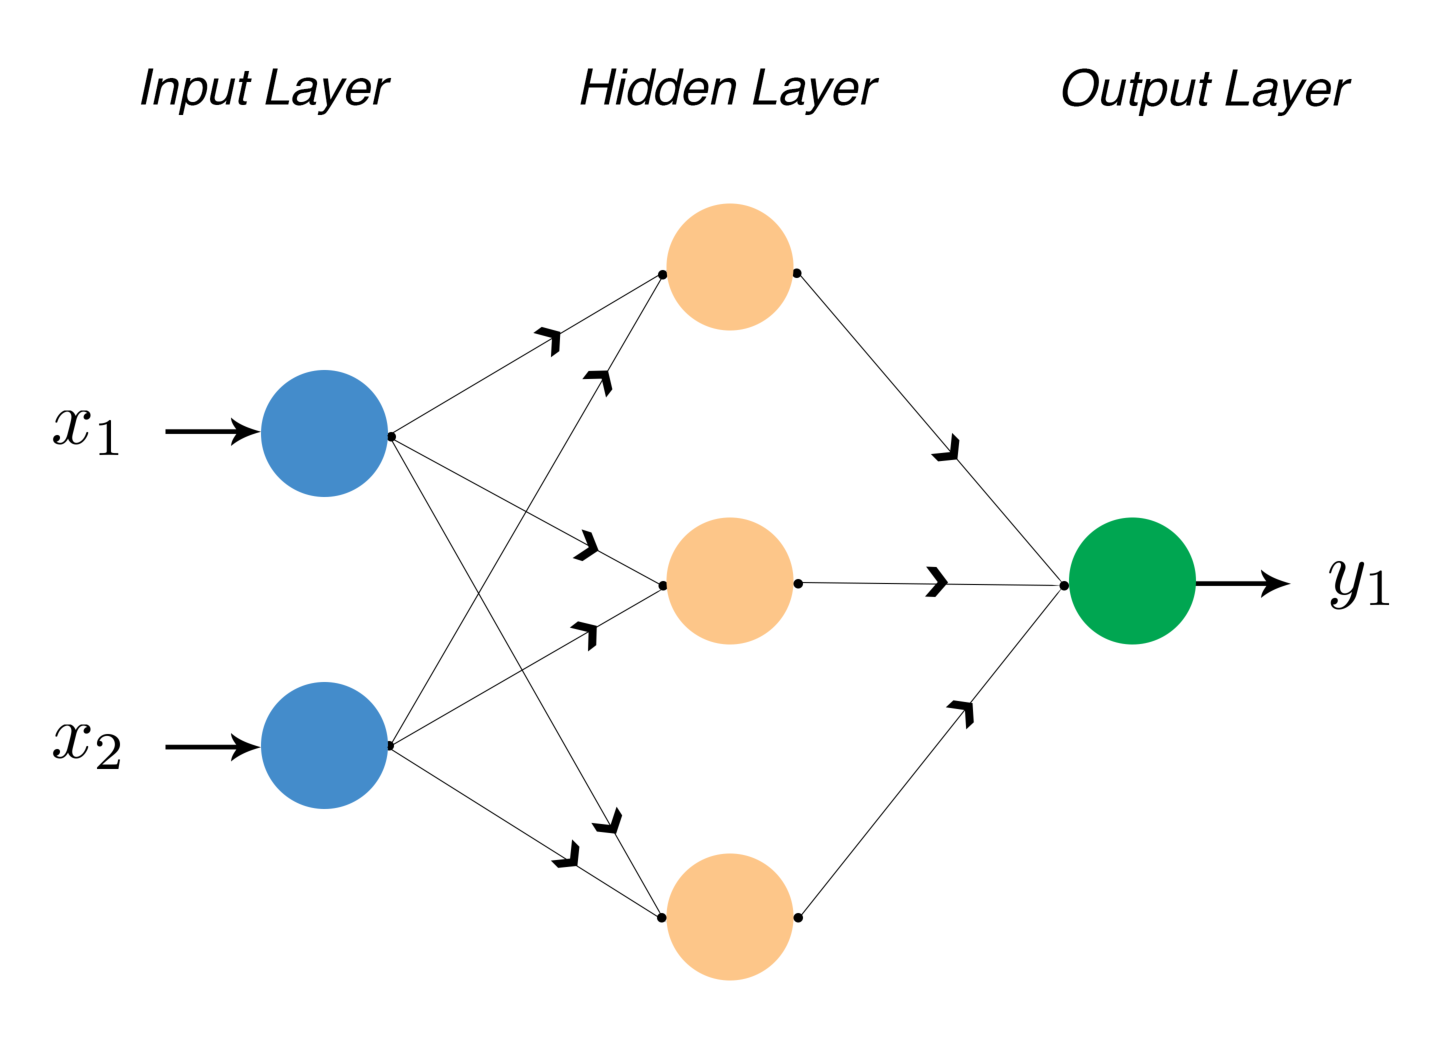
\includegraphics[width
%    =0.4\textwidth]{schematic_toy_network.pdf}
%    \caption{A schematic diagram showing a simple %artificial neural network with a single hidden %layer. Image reproduced from %\cite{Ghosh2020GalaxyGalaxies}.}
%    \label{fig_c2:toy_network_schematic}
%\end{figure}

The %form of artificial neural network that forms the 
backbone of \gampen{} is a Convolutional Neural Network (\citealp{fukushima_80, lecun_98}). %While traditional artificial neural networks learn global patterns in their input feature space, CNNs learn to identify thousands of local patterns in their input images that are translation invariant. 
Without convolutional layers, neural networks learn global patterns, whereas CNNs learn to identify thousands of local patterns in their input images that are translation invariant.
Additionally, CNNs learn the spatial hierarchies of these patterns, allowing them to process increasingly complex and abstract visual concepts. These two key features have allowed deep CNNs to revolutionize the field of image processing in the last decade \citep{lecun_15, dl_overview}. 

\begin{figure*}[htb]
    \centering
    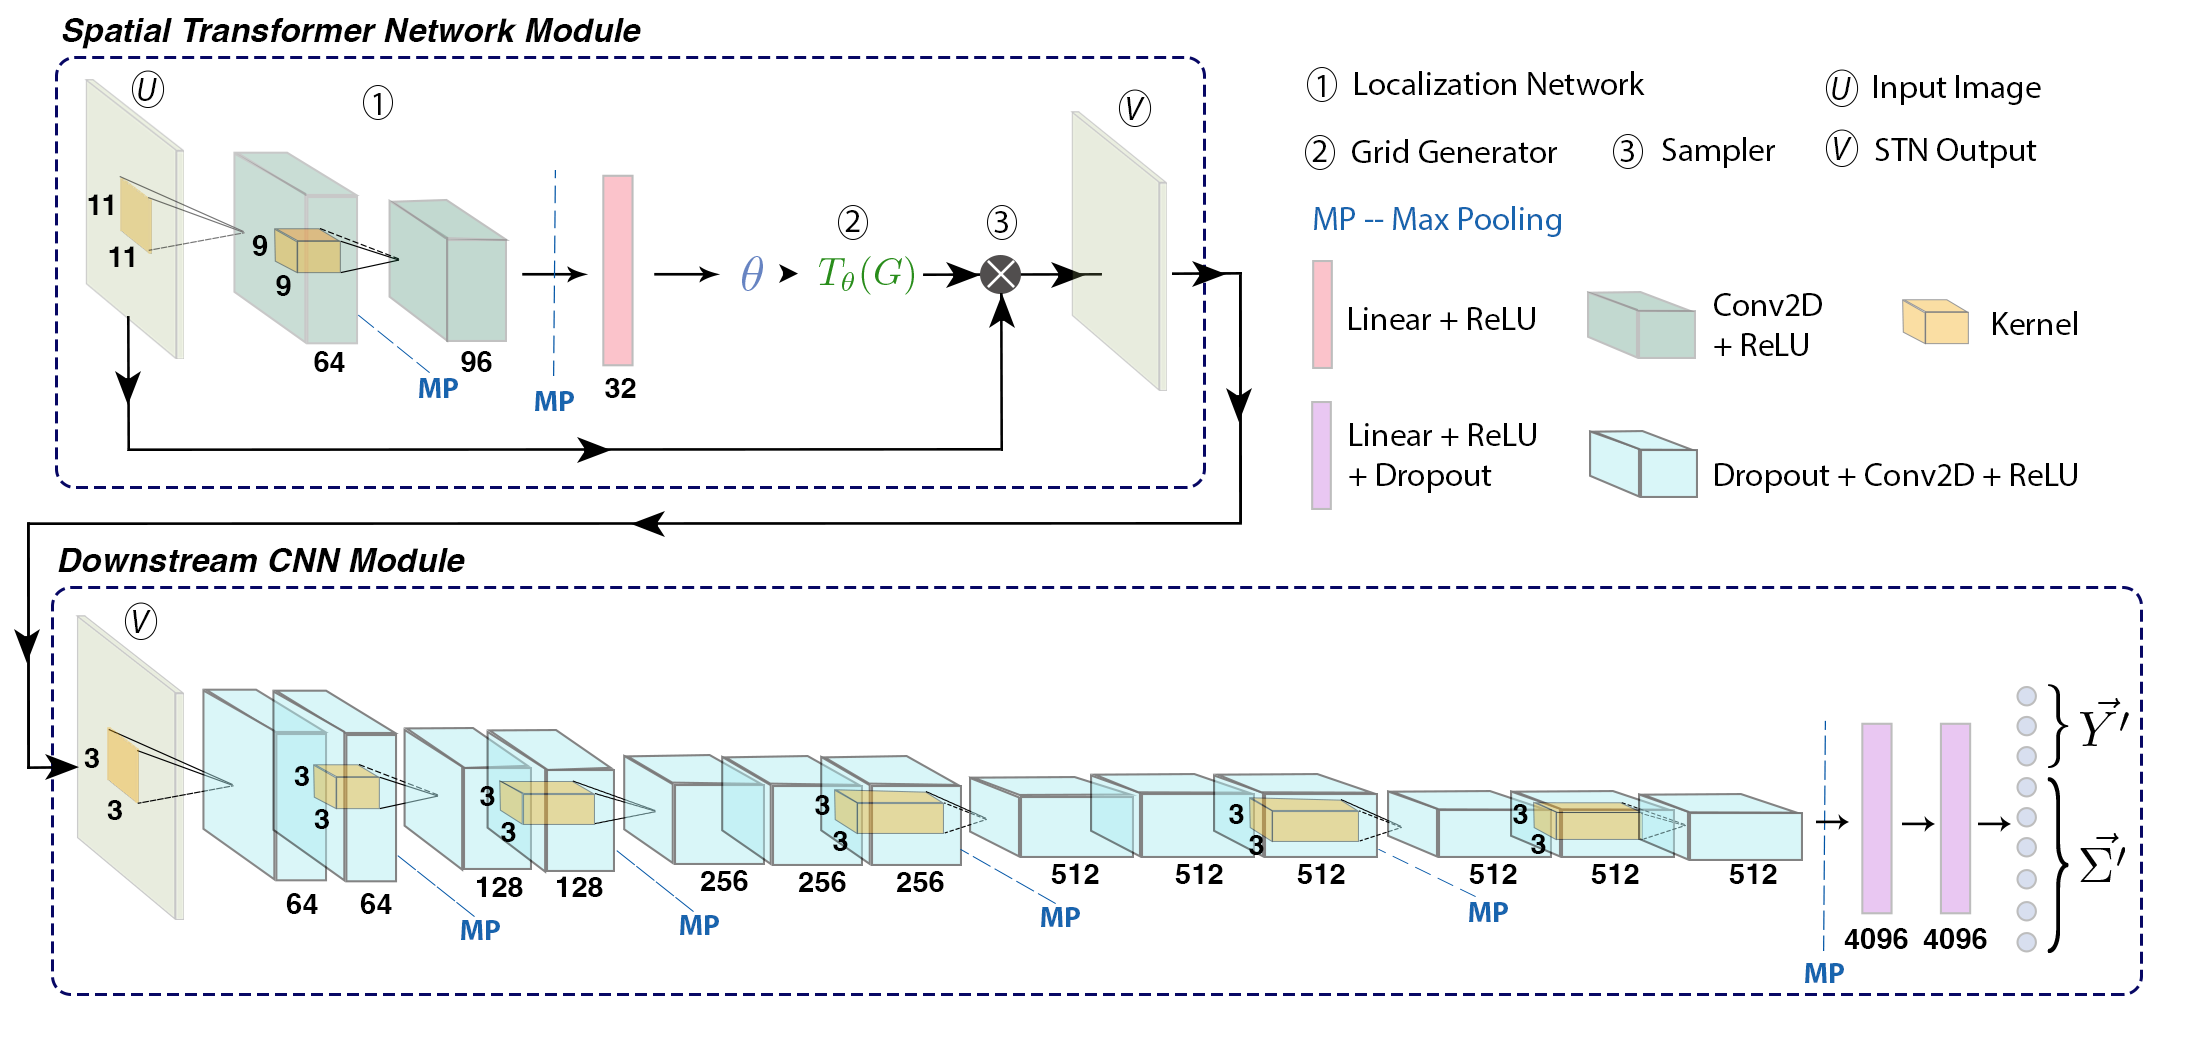
\includegraphics[width
    =\textwidth]{gampen_schematic.png}
    \caption{A schematic diagram of the Galaxy Morphology Posterior Estimation Network. \gampen's architecture consists of a downstream CNN module preceded by an upstream STN module. The CNN module empowers \gampen{} to estimate posterior distributions of galaxy morphology parameters. The upstream STN module trains without any extra supervision and learns to apply appropriate cropping transformations to the input image before passing it on to the CNN (for more details about these modules, see \S\S\,\ref{subsec_c2:STN}, \ref{subsec_c2:cnn}).
    The numbers below each layer refer to the number of filters/neurons in each layer. The yellow boxes inside the convolutional layers show the kernel and the number beside it refers to the corresponding kernel size. Only one kernel is shown per set of convolutional layers; all other layers in the set have kernels of the same size. Conv2D and ReLU refer to Convolutional Layers and Rectified Linear Units, respectively (described in \S.\ref{subsec_c2:cnn}).}
    \label{fig_c2:gampen_schematic}
\end{figure*}


The architecture of \gampen{} is shown in Figure\,\ref{fig_c2:gampen_schematic}. It consists of a Spatial Transformer Network module followed by a downstream CNN module, described in \S\,\ref{subsec_c2:STN} and \ref{subsec_c2:cnn}, respectively. The design of \gampen{} is based on our previously successful classification CNN, \gamornet{} \citep{Ghosh2020GalaxyGalaxies}, as well as different variants of the Visual Geometry Group (VGG) networks \citep{vgg}, which are highly effective at large-scale visual recognition. We tried different architectures of these ``base" models by varying the depth of the entire network and the sizes of the various layers. To quickly and systematically search this model-design space, we use ModulosAI's\footnote{\href{https://www.modulos.ai}{https://www.modulos.ai}} AutoML platform, which uses a Bayesian optimization strategy. The said strategy involves using the current model's performance to determine which variant to try next. When choosing new configurations, the optimizer balances the exploitation of well-performing search spaces and the exploration of unknown regions.

To implement \gampen{}, we use PyTorch,
%\footnote{\href{https://pytorch.org}{https://pytorch.org}}
 which is an open-source machine learning framework, written in Python.

\subsection{The Spatial Transformer Network Module } \label{subsec_c2:STN}
Spatial Transformer Networks (STNs) were introduced by \cite{jarderberg_15} as a learnable module that can be inserted into CNNs and explicitly allows for the spatial manipulation of data within the CNN. In the astronomical context, STNs have only been used by \cite{wu_2019} previously in morphological analysis of radio data. 

In \gampen{}, the STN is upstream of the CNN, where it applies a two-dimensional affine transformation to the input image, and the transformed image is then passed to the CNN. 
%The transformation applied by the STN depends on the specific input image, and the STN 
Each input image is transformed differently by the STN, which 
learns the appropriate cropping during the training of the downstream CNN without additional supervision. As shown in the upper part of Figure \ref{fig_c2:gampen_schematic}, the STN consists of (1) a localization network, (2) a parameterized grid generator, and (3) a sampler, as described below.

\begin{figure*}[htb]
    \centering
    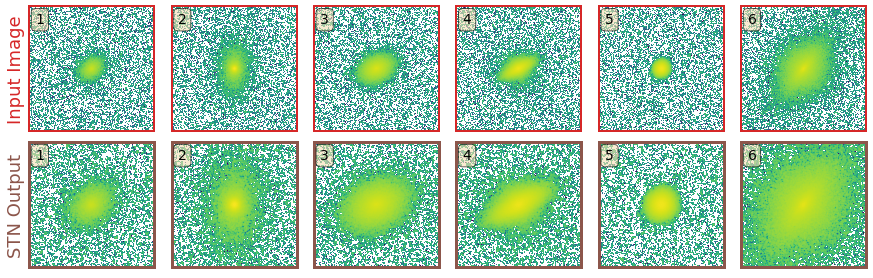
\includegraphics[width
    =\textwidth]{stn_examples.png}
    \caption{Examples of the transformation applied by the STN to six randomly selected input galaxy images. The top row shows the input galaxy images, and the bottom row shows the corresponding output from the STN. The numbers in the top-left yellow boxes help correspond the output images to the input images. As can be seen, the STN learns to apply an optimal amount of cropping for each input galaxy.}
    \label{fig_c2:stn_examples}
\end{figure*}

The localization network takes the input image, $U$ ($U \in \mathbb{R}^{H \times W \times C}$, with height $H$, width $W$, and $C$ channels), and outputs $\boldsymbol{\theta}$, the six-parameter matrix of the affine transformation, $\mathcal{T}_\theta$, to be applied to the input image.
%\boldsymbol{\theta}4=f_{\mathrm{loc}}(U)$. 
The localization network in the STN is a CNN with two convolutional layers followed by two fully connected layers at the end. 

%Next, the parameterized sampling grid helps to apply the transformation $\mathcal{T}_\theta$ to the input image. To transform the input image, the output pixels are computed by applying a sampling kernel on the input image. 

To perform the transformation, $\mathcal{T}_\theta$, the values of the output pixels are computed by applying a sampling kernel on the input image. As the first step in this process, the parameterized grid generator is used to generate a grid, $G$, of target coordinates, $ G_i =  \left( x_i^t, y_i^t \right) $, forming the output of the STN. For our case, $\mathcal{T}_\theta$ is a 2D affine transformation $A_{\theta}$, and the pointwise transformation is given by

\begin{equation}
\begin{split}
\left(\begin{array}{c}
x_{i}^{s} \\
y_{i}^{s}
\end{array}\right)=\mathcal{T}_{\theta}\left(G_{i}\right) & = \mathrm{A}_{\theta}\left(\begin{array}{c}
x_{i}^{t} \\
y_{i}^{t} \\
1
\end{array}\right) \\
& = \left[\begin{array}{lll}
\theta_{11} & \theta_{12} & \theta_{13} \\
\theta_{21} & \theta_{22} & \theta_{23}
\end{array}\right]\left(\begin{array}{c}
x_{i}^{t} \\
y_{i}^{t} \\
1
\end{array}\right) ,
\end{split}
\label{eq:stn_transformation}
\end{equation}

\noindent
where $ \left(x_i^s,y_i^s\right)$ are the source coordinates in the input image that define the sample points \citep{jarderberg_15}. The transformation shown in Equation\,\ref{eq:stn_transformation} allows for cropping, translation, rotation, and skewing to be applied to the input image. However, the simulated galaxy images in our dataset are already centered, and our primary aim of using the STN is to achieve optimal cropping; thus, we constrain the type of affine transformations allowed by modifying $\mathrm{A}_{\theta}$ such that 

\begin{equation}
\mathrm{A}_{\theta} = \left[\begin{array}{lll}
s & 0 & 0 \\
0 & s & 0
\end{array}\right] .
\label{eq:cropping_transformation}
\end{equation}

\noindent
The localization network predicts the optimal value of $s$ for each input image. As can be seen from Eq. \ref{eq:cropping_transformation}, $s=1$ results in an identity transformation (i.e., the image output by the STN and the input image are the same). For values of $s < 1$, lower fractions of the input image are retained in the output image. For example, when $s=0.7$, $70\%$ of each side (length/width) of the input image is retained in the output image.

Note that although \gampen{}'s STN does not perform rotations, we are able to induce rotational invariance using our training procedure.  Since our simulated training set is very large, it happens to be that there are many galaxies with different position angles, but similar (other) structural parameters.

In the final step, the sampler takes the set of sampling points $\mathcal{T}_\theta(G)$ along with the input image, $U$, to produce the output image, $V$. Each $ \left(x_i^s,y_i^s\right)$ coordinate in $\mathcal{T}_\theta(G)$ defines the spatial location in the input where a bilinear sampling kernel is applied to get the value at a particular pixel in the output image. This can be written as 

\begin{equation}
\begin{split}
V_{i}^{c}=\sum_{n}^{H} \sum_{m}^{W} U_{n m}^{c} & \max \left(0,1-\left|x_{i}^{s}-m\right|\right) \times \\ & \max \left(0,1-\left|y_{i}^{s}-n\right|\right) , 
\end{split}
\label{eq:smapling_v}
\end{equation}

\noindent
where $U_{n m}^{c}$ is the value at location ($n$,$m$) in channel $c$ of the input, and $V_{i}^{c}$ is the output value for pixel $i$ at location $\left(x_i^t,y_i^t\right)$ in channel $c$. To allow the backpropagation of the loss through this sampling mechanism, we can define the gradients with respect to $U$ and $G$. This allows loss gradients to flow back to the sampling grid coordinates and therefore back to the transformation parameter $s$ and the localization network.

Placing the STN upstream in the \gampen{} framework allows the network to learn how to actively transform the input image to minimize the overall loss function during training. Because the transformation we use is differentiable with respect to the parameters, gradients can be backpropagated through the sampling points $\mathcal{T}_\theta(G)$ to the localization network output $\boldsymbol{\theta}$. This crucial property allows the STN to be trained using standard backpropagation along with the downstream CNN, without any additional supervision. 

Figure \ref{fig_c2:stn_examples} shows examples of the transformations applied by the STN of a trained \gampen{} framework to simulated HSC data. As can be seen, the STN learns to apply an optimal amount of cropping for each input galaxy. 

\begin{figure*}[htb]
    \centering
    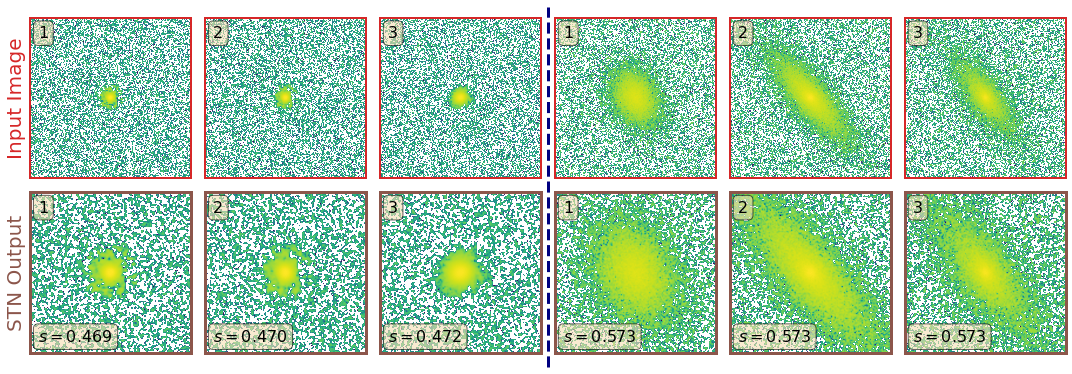
\includegraphics[width
    =\textwidth]{most_least_crops.png}
    \caption{(\textit{Left}): Galaxies in the testing dataset with the lowest values of $s$ (i.e., the most aggressive crops) (\textit{Right}): Galaxies in the testing dataset with the highest values of $s$ (i.e., the least aggressive crops). As can be seen, the STN correctly learns to apply the most aggressive crops to small galaxies; and the least aggressive crops to large galaxies.}
    \label{fig_c2:most_least_crops}
\end{figure*}

To further validate the performance of our STN, we process all images in our testing dataset through the STN module of a trained \gampen{} framework. After that, we sort all the processed images using the value of the parameter $s$ (from Eq. \ref{eq:cropping_transformation}) predicted by the localization network. Higher values of $s$ denote that a more significant fraction of the input image was retained in the output image produced by the STN  (i.e., minimal cropping). In Figure \ref{fig_c2:most_least_crops}, we show the images from our testing dataset with the highest and lowest values of $s$. Figure \ref{fig_c2:most_least_crops} demonstrates that the STN correctly learns to apply the most aggressive crops to smallest galaxies in our dataset, and the least aggressive crops to the largest galaxies.

\begin{figure}[htb]
    \centering
    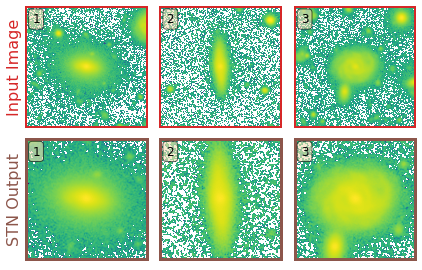
\includegraphics[width
    =0.45\textwidth]{real_galaxies_stn.png}
    \caption{Examples of the transformation applied by a trained STN to real HSC-Wide \textit{g}-band galaxies. The STN helps the downstream CNN to focus on the galaxy of interest at the center of the cutout by cropping out most secondary galaxies present in the input frame.}
    \label{fig_c2:real_galaxies_stn}
\end{figure}

Lastly, in order to demonstrate the purpose of including an STN in \gampen{}, we show its performance on real HSC galaxies. We apply the STN module of a trained \gampen{} framework to three randomly chosen \textit{g}-band galaxies in the HSC-Wide survey with $z \leq 0.25$ and $m_g \leq 23$. Each input image is $40 \times 40$ arcsec. (Note that, for this demonstration, we did not retrain \gampen{} on real galaxies in any way.) The results are shown in Figure\,\ref{fig_c2:real_galaxies_stn}. The STN learns to systematically crop out secondary galaxies in the cutouts and focus on the galaxy of interest at the center of the cutout. At the same time, the STN also correctly applies minimal cropping to the largest galaxies, making sure the entirety of these galaxies remains in the frame. 

\subsection{The Convolutional Neural Network Module} \label{subsec_c2:cnn}

The input image, once transformed by the STN, is passed to the downstream CNN module, as depicted in Figure \ref{fig_c2:gampen_schematic}. This downstream module predicts the posterior distribution of the bulge-to-total light ratio, effective radius, and total flux for each input galaxy. 

The architecture of this downstream CNN is based on the design of VGG-16 \citep{vgg}, a CNN that performed well in the 2014 ImageNet Large Scale Visual Recognition Challenge, wherein different teams compete to classify about 14 million hand-annotated images. The primary feature of the VGG class of networks is that they use tiny convolutional filters combined with significantly deep networks, which have been shown to be highly successful in computer vision. Broadly speaking, \gampen{}'s downstream CNN consists of thirteen convolutional layers, followed by three fully connected layers. The convolutional layers are arranged in five blocks, and in between each block is a max-pooling layer. Note that one of the primary differences between our network and VGG-16 is that all the convolutional layers in \gampen{} are preceded by a dropout layer in order to facilitate the prediction of epistemic uncertainties, as described further in \S \ref{subsec_c2:mcd}. 

The convolutional layers (Conv2D in Fig. \ref{fig_c2:gampen_schematic}) work in unison to identify hierarchies of translational invariant spatial patterns in the images. Each convolutional layer does this by using a collection of $3\times3$ pixel windows (called ``filters"), wherein each filter is a specific pattern that the CNN is looking for in the image. These windows slide around the input to generate a ``response-map" or ``feature-map", which quantifies the presence of the filter's pattern at different locations of the input. Each convolutional layer is preceded by a dropout layer, which is one of the most effective and commonly used regularization techniques that prevent over-fitting by randomly ``dropping" (i.e., setting to zero) several output features of the layer during training. The ``dropout rate" defines the fraction of features that are zeroed out. For \gampen{}, our choice of the dropout rate is guided by calibration of the predicted uncertainties and is described in \S \ref{sec_c2:training}.

The goal of the max-pooling layers (MP in Fig. \ref{fig_c2:gampen_schematic}) is to aggressively down-sample the outputs of the convolutional layer that they follow. Simply speaking, max-pooling is dividing the output of the convolutional layer into a collection of windows and then using the maximum value in each window as the output. Max-pooling can be thought of as a technique for detecting a given feature in a broad region of the image and then throwing away the exact positional information. The intuition is that once a feature has been found, its exact location is not as crucial as its rough location relative to other features. An additional advantage is that by aggressively down-sampling, max-pooling forces successive convolutional layers to look at increasingly large windows as a fraction of the input to the layer. This helps to induce spatial-filter hierarchies. 

Throughout the network, we use the rectified linear unit (ReLU in Fig. \ref{fig_c2:gampen_schematic}) as the activation function, except for the output layer, which is linear. The output of a ReLU unit with input $\mathbf{x}$, weight $\mathbf{w}$, and bias $b$ is given by $\max (0, \boldsymbol{w} \cdot \boldsymbol{x}+b)$. The application of the ReLU activation function makes the network non-linear. 

At the end of the network are three fully connected layers. They use the output of the convolutional layers, denoting the presence of various features in the image, to predict the correct output variables given an image. The output layer predicts nine parameters. Three of these construct the vector of means of the output variables $(\boldsymbol{\hat{\mu}})$, and the remaining six are used to construct the covariance matrix $\boldsymbol{\hat{\Sigma}}$. In \S\,\ref{sec_c2:uncertainties}, we describe more about how these two variables are used to generate the predicted distributions.

Table \ref{tab_c2:network_layers} in the Appendix gives extended descriptions of each \gampen\ layer. 
For more technical details about the various layers and functions described there, we refer the reader to \cite{nielsen,goodfellow_16,chollet_21}.


\section{Prediction of Posteriors} \label{sec_c2:uncertainties}
Traditional CNNs consist of neurons with fixed, deterministic values of weights and biases, resulting in deterministic outputs. However, if the weights in such a network are probability distributions, then the calculation can be defined within a Bayesian framework \citep{denker_91}. Such CNNs can then be used to capture the posterior probabilities of the outputs, resulting in well-defined estimates of uncertainties. The key distinguishing property of the Bayesian approach is marginalization over multiple networks rather than a single optimization run. 

Two primary sources of error contribute to the uncertainties in the parameters predicted by \gampen{}. The first arises from errors inherent to the input imaging data (e.g., noise and PSF blurring), and this is commonly referred to as aleatoric uncertainty. The second error comes from the limitations of the model being used for prediction (e.g., the number of free parameters in \gampen{}, the amount of training data, etc.); this is referred to as epistemic uncertainty. It is important to note that while epistemic uncertainties can be reduced with proper changes to the model (e.g., more training data, more flexible model), aleatoric uncertainties are determined by the input images and thus cannot be reduced. There has been much recent work on how to estimate uncertainties efficiently in deep learning \citep[e.g.,][]{gal_2016,Kendall2017WhatVision,Pawlowski2017ImplicitNetworks,Wilson2020BayesianGeneralization} and some of these techniques have also been applied to astrophysical problems \citep[e.g.,][]{PerreaultLevasseur2017UncertaintiesLensing, Walmsley2020GalaxyLearning, Wagner-Carena2021HierarchicalLensing, Cranmer2021ASystems}. The following two sections describe how we arrange for \gampen\ to estimate both parameter values and their uncertainties.
%as well as model para into the \gampen{} predictions. 

\subsection{Bayesian Implementation of \gampen{} and Epistemic Uncertainties} \label{subsec_c2:mcd}
To create a Bayesian framework while predicting morphological parameters, we have to treat the model itself as a random variable---or more precisely, the weights of our network %, $\boldsymbol{\omega}$, 
must be probabilistic distributions instead of single
%deterministic 
values. For a network with weights, $\boldsymbol{\omega}$, and a training dataset, $\mathcal{D}$, of size $N$ with input images $\left\{\boldsymbol{X}_{1}, \ldots, \boldsymbol{X}_{N}\right\}$ and output parameters $\left\{\boldsymbol{Y}_{1}, \ldots, \boldsymbol{Y}_{N}\right\}$, the posterior of the network weights, $p(\boldsymbol{\omega} \mid \left\{\boldsymbol{X}_{1}, \ldots, \boldsymbol{X}_{N}\right\}, \left\{\boldsymbol{Y}_{1}, \ldots, \boldsymbol{Y}_{N}\right\}) \equiv p(\boldsymbol{\omega} \mid \mathcal{D}) $ represents the plausible network parameters. To predict the probability distribution of the output variable $\boldsymbol{\hat{Y}}$ given a new test image $\boldsymbol{\hat{X}}$, we need to marginalize over all possible weights $\boldsymbol{\omega}$:

\begin{equation}
p(\boldsymbol{\hat{Y}} \mid \boldsymbol{\hat{X}}, \mathcal{D})=\int p(\boldsymbol{\hat{Y}} \mid \boldsymbol{\hat{X}}, \boldsymbol{\omega}) p(\boldsymbol{\omega} \mid \mathcal{D}) d \boldsymbol{\omega} .
\label{eq:out_y_pred}
\end{equation}

In order to calculate the above integral, we need to know $p(\boldsymbol{\omega}\mid\mathcal{D})$, i.e., how likely is a particular set of weights given the available training data, $\mathcal{D}$. Since we have trained only the one model, it does not tell us how likely different sets of weights are. Different approximations have been introduced in order to calculate this distribution, with variational inference \citep{Jordan1999IntroductionModels} being the most popular.

Now, the dropout technique was introduced by \cite{Srivastava2014Dropout:Overfitting} in order to prevent neural networks from overfitting; they temporarily removed random neurons from the network according to a Bernoulli distribution, i.e., individual nodes were set to zero with a probability, $p$, known as the dropout rate. This dropout process can also be interpreted as taking the trained model and permuting it into a different one \citep{Srivastava2014Dropout:Overfitting}.

Using variational inference and dropout, we can approximate the integral in Equation \ref{eq:out_y_pred} as 

\begin{equation}
\int p(\boldsymbol{\hat{Y}} \mid \boldsymbol{\hat{X}}, \boldsymbol{\omega}) p(\boldsymbol{\omega} \mid \mathcal{D}) d \boldsymbol{\omega} \approx \frac{1}{T} \sum_{t=1}^{T} p(\boldsymbol{\hat{Y}} \mid \boldsymbol{\hat{X}}, \boldsymbol{\omega}_t) ,
\label{eq:mcd_final}
\end{equation}

\noindent
wherein we perform $T$ forward passes with dropout enabled and $\boldsymbol{\omega}_t$ is the set of weights during the $t$\textsuperscript{th} forward pass. This procedure is what is referred to as Monte Carlo Dropout. For a detailed derivation of Equation \ref{eq:mcd_final}, please refer to Appendix \ref{sec_c2:ap:mcd_deri}

In order to obtain epistemic uncertainties for \gampen{}, we insert a dropout layer before every weight layer in the network. Each forward pass through \gampen{} samples the approximate parameter posterior. Thus, in order to obtain epistemic uncertainties, we feed every test image $\boldsymbol{\hat{X}}_i$ to the trained \gampen{} framework $T$ times and collect the outputs. In implementing the Monte Carlo Dropout technique, an often-ignored key step is tuning the dropout rate (i.e., the rate at which neurons are set to zero). We discuss the tuning of the dropout rate for \gampen{} in \S \ref{sec_c2:training}.

\vspace{0.8cm}


\subsection{Likelihood Calculation and Aleatoric Uncertainties}
\label{subsec_c2:aleatoric}
Our simulated training data consists of noisy input images by design, but we know the corresponding morphological parameters with perfect accuracy. However, due to the different amounts of noise in each image, the predictions of \gampen{} at test time should have different levels of uncertainties. Thus, in this situation, we want to use a heteroscedastic model -- a model that can capture different levels of uncertainties in its output predictions. We achieve this by training \gampen{} to predict the aleatoric uncertainties. 

As outlined in \S \ref{sec_c2:training}, \gampen{} predicts a multivariate log-normal distribution of output variables for any given input image. Thus, for a given set of network weights $\boldsymbol{\omega}$, the likelihood $p(\mathcal{D} \mid \boldsymbol{\omega})$ is simply the product of the probabilities that the \gampen{} output for each image is drawn from the associated multivariate Gaussian distribution $\mathcal{N}(\boldsymbol{\mu}, \boldsymbol{\Sigma})$ in $\mathbf{R^3}$ , with mean $\boldsymbol{\mu}$ and covariance matrix $\boldsymbol{\Sigma}$.

Although we would like to use \gampen{} to predict aleatoric uncertainties, the covariance matrix, $\boldsymbol{\Sigma}$, is not known {\it a priori}. Instead, we train \gampen{} to learn these values by minimizing the negative log-likelihood of the output parameters for the training set, which can be written as

\begin{equation}
\begin{split}
- \log \mathcal{L}_{VI} \propto  \sum_{n} & \frac{1}{2}\left[\boldsymbol{Y}_{n}-\boldsymbol{\hat{\mu}}_{n}\right]^{\top} \boldsymbol{\hat{\Sigma_n}}^{-1}\left[\boldsymbol{Y}_{n}-\boldsymbol{\hat{\mu}}_{n}\right] \\ 
& + \frac{1}{2} \log [\operatorname{det}(\boldsymbol{\hat{\Sigma_n}})] + \lambda \sum_{i}\left\|\boldsymbol{\omega_{i}}\right\|^{2} .
\end{split}
\label{eq:final_loss_fn}
\end{equation}

where $\boldsymbol{\hat{\mu}}_n$ and $\boldsymbol{\hat{\Sigma}}_n$ are the mean and covariance matrix of the multivariate Gaussian distribution predicted by \gampen{} for an image, $\boldsymbol{X}_n$. $\lambda$ is the strength of the regularization term, and $\boldsymbol{\omega}_i$ are sampled from $q(\boldsymbol{\omega})$. For a detailed derivation of Equation \ref{eq:final_loss_fn}, we refer an interested reader to Appendix \ref{sec_c2:ap:final_loss_deri}.

The covariance matrix here represents the uncertainties in the predicted parameters arising from inherent corruptions to the input or the output data. Note that using the full covariance matrix in Equation \ref{eq:final_loss_fn} instead of just the diagonal terms (i.e., assuming the output variables to be independent), helps \gampen{} to incorporate the structured relationship between the different output parameters. We further outline the effects of this in \S \ref{sec_c2:training}.


\subsection{Practical Implementation Details} \label{subsec_c2:uncertainty_implementation}

In order to predict $\boldsymbol{\mu}$ and $\boldsymbol{\Sigma}$, the final layer of \gampen{} contains nine output nodes (see Fig.\,\ref{fig_c2:gampen_schematic}). Three of these nodes are used to characterize $\boldsymbol{\mu}$. % = \mu_{k=1}^3$, where $k$ represents each output variable. 
Now, although $\boldsymbol{\Sigma}$ is a $3\times3$ matrix, we are able to characterize it with just six parameters due to its special properties. Because $\boldsymbol{\Sigma}$ is a symmetric, positive-definite matrix, we can use the LDL decomposition, a variant of the Cholesky decomposition \citep{cholesky}, to represent 

\begin{equation}
\boldsymbol{\Sigma} = \left(\begin{array}{ccc}
\sigma_{1}^{2} & \sigma_{12} & \sigma_{13} \\
\sigma_{21} & \sigma_{2}^{2} & \sigma_{23} \\
\sigma_{31} & \sigma_{32} & \sigma_{3}^{2}
\end{array}\right)
\label{eq:full_sigma_matrix}
\end{equation}

\noindent
as $\boldsymbol{\Sigma} = \boldsymbol{L}\boldsymbol{D}\boldsymbol{L}^{\top}$, where 

\begin{equation}
\boldsymbol{L} = \left(\begin{array}{lll}
1 & 0 & 0 \\
\sigma_{21} & 1 & 0 \\
\sigma_{31} & \sigma_{32} & 1
\end{array}\right)
\label{eq:form_of_L}
\end{equation}

\noindent
and 

\begin{equation}
D=\left(\begin{array}{ccc}
\sigma_{1}^{2} & 0 & 0 \\
0 & \sigma_{2}^{2} & 0 \\
0 & 0 & \sigma_{3}^{2}
\end{array}\right) .
\label{eq:form_of_D}
\end{equation}

\noindent
Thus, three of \gampen{}'s output nodes are used to predict the off-diagonal elements in Equation\,\ref{eq:form_of_L},
%$\sigma_{i>j\geq1}^{3}\sigma_{i,j}$ 
and three more are used to predict $_{i=1}^3s_i$ where $s_i=\log(\sigma_i^2)$. We predict $s_i$ instead of $\sigma_i^2$ in order to achieve better numerical stability during training. 

The loss function, outlined in Equation \ref{eq:final_loss_fn}, contains the determinant and the inverse of $\boldsymbol{\Sigma}$. Calculation of the determinant and the inverse of a matrix are potentially numerically unstable and slow operations. Thus, in order to achieve the maximum speed possible on our GPUs and for numerical stability, we replace these operations using the Cholesky decomposition outlined above and standard linear algebra. 
That is, $\boldsymbol{\Sigma}^{-1}$ can be written as $\boldsymbol{\Sigma}^{-1}=\left(\boldsymbol{L}^{-1}\right)^{\top} \boldsymbol{D}^{-1} \boldsymbol{L}^{-1}$, where 

\begin{equation}
\boldsymbol{D}^{-1}=\left(\begin{array}{ccc}
\frac{1}{\sigma_{1}^{2}} & 0 & 0 \\
0 & \frac{1}{\sigma_{2}^{2}} & 0 \\
0 & 0 & \frac{1}{\sigma_{3}^{2}}
\end{array}\right)
\label{eq:D_inv}
\end{equation}

\noindent
because $\boldsymbol{D}$ is a diagonal matrix. Because $\boldsymbol{L}$ is a lower triangular matrix, we can also write its inverse as  

\begin{equation}
\boldsymbol{L}^{-1}=(\boldsymbol{I}+\boldsymbol{N})^{-1}= \boldsymbol{I} +\sum_{k=1}^{2}(-1)^{k} \boldsymbol{N}^{k} ,
\label{eq:L_inv}
\end{equation}

\noindent
where $\boldsymbol{I}$ is a $3\times3$ identity matrix and $\boldsymbol{N}$ is a strictly lower triangular and nilpotent matrix such that $\boldsymbol{N} = \boldsymbol{L} - \boldsymbol{I}$.

Finally, we can write the $\log (\operatorname{det}(\boldsymbol{\Sigma}))$ as

\begin{equation}
\begin{split}
\log (\operatorname{det}(\boldsymbol{\Sigma})) 
& = \log (\operatorname{det} (\boldsymbol{L}\boldsymbol{D}\boldsymbol{L}^{\top})) \\
& = \log (\prod_i D_{ii}) \\
& = \sum \log D_{ii} .
\end{split}
\label{eq:log_det_sigma}
\end{equation}

\noindent
By combining Equations \ref{eq:D_inv}, \ref{eq:L_inv}, and \ref{eq:log_det_sigma}, we can calculate the log-likelihood outlined in Equation \ref{eq:final_loss_fn} without having to calculate the inverse or determinant of any matrix, allowing us to fully utilize the capabilities of a GPU and avoiding any numerical instabilities. 

\begin{figure*}[htb]
    \centering
    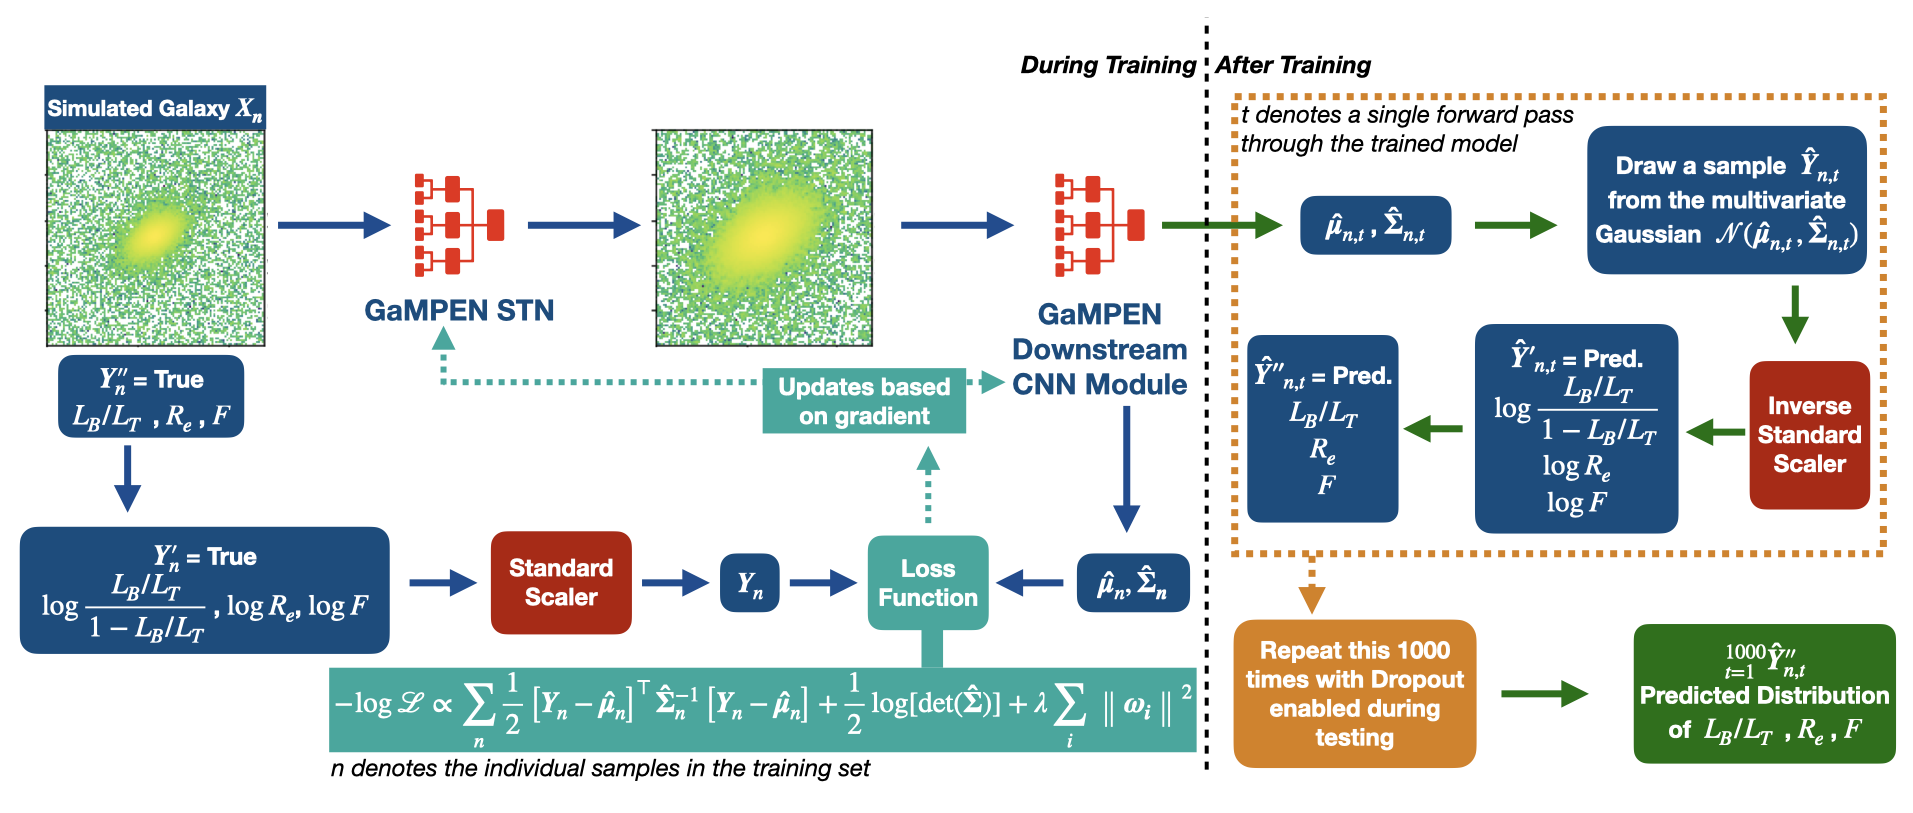
\includegraphics[width
    =\textwidth]{workflow_gampen.png}
    \caption{Diagram outlining the training (\textit{left}) and inference (\textit{right}) phases of the \gampen\ workflow. Training consists of feeding 105,000 simulated images (with known parameter values) through the STN and CNN modules, minimizing the loss function (Eqn.\,\ref{eq:final_loss_fn}) using Stochastic Gradient Descent. 
    During this process, we re-scale the variables as described in the text, and return them to the original variable space during inference.
    After the STN+CNN are trained, the inference step consists of 1000 forward passes with dropout enabled for each galaxy image. We draw a sample from the predicted multivariate Gaussian distribution during each forward pass, and the collection of these samples gives us the predicted posterior distribution.}
    \label{fig_c2:workflow}
\end{figure*}

\subsection{Combining Aleatoric and Epistemic Uncertainties}
\label{subsec_c2:combining_uncertainties}
To obtain the posterior distribution of the output variables, we need to combine the aleatoric and epistemic uncertainties. After training a model by maximizing the log-likelihood outlined in Equation \ref{eq:final_loss_fn}, we perform Monte Carlo Dropout. To do this, as outlined in Figure \ref{fig_c2:workflow}, we feed each input image, $\boldsymbol{\hat{X}}_n$, in the test set 1000 times into \gampen{} with dropout enabled. During each iteration, we collect the predicted set of $\left(\hat{\boldsymbol{\mu}}_{n,t},\boldsymbol{\hat{\Sigma}}_{n,t}\right)$ for the $t^{th}$ forward pass. Then, for each forward pass, we draw a sample $\boldsymbol{\hat{Y}_{n,t}}$ from the multivariate normal distribution $\mathcal{N}\left(\boldsymbol{\hat{\mu}}_{n,t},\boldsymbol{\hat{\Sigma}}_{n,t}\right)$. 

The distribution generated by the collection of all 1000 forward passes, $\boldsymbol{\hat{Y}_{n}}$,
%$_{t=1}^{1000}\boldsymbol{\hat{Y}_{n,t}}$ 
represents the predicted posterior distribution for the test image $\boldsymbol{\hat{X}}_n$. The different forward passes capture the epistemic uncertainties, and each prediction in this sample also has its associated aleatoric uncertainty represented by $\boldsymbol{\hat{\Sigma}_{n,t}}$. Thus the above procedure allows us to incorporate both aleatoric and epistemic uncertainties in the prediction of posteriors of morphological parameters by \gampen{}.

\section{Training \gampen } \label{sec_c2:training}
We split the dataset of 150,000 simulated galaxies into training, validation, and testing sets with $70\%$, $15\%$, and $15\%$ of the total sample, respectively. We train \gampen{} using the training set, and set the values of various hyper-parameters (e.g., learning rate, batch size; see below) using the validation set. Finally, we evaluate the trained model on the testing set (which has never been seen before by the network) and report the results in \S \ref{sec_c2:results}.

We pass all the images in the simulated dataset through the arsinh function to reduce the dynamic range of pixel values in the images. This function behaves linearly around zero and logarithmically for large values. Reducing the dynamic range of pixel values has been found to be helpful in neural network convergence \citep[e.g.,][]{zanisi_21,walmsley_decals,tanaka_22}, hence this approach. 

The three output variables that we predict with \gampen{} have quite different ranges, by orders of magnitude. Thus, we re-scale these ground-truth training values before feeding them into the network in order to prevent variables with larger numerical values from making a disproportionate contribution to the loss function. Additionally, we also need to make sure that none of the values predicted by \gampen{} happen to be unphysical; that is, we require all output values to adhere to the following ranges: $0 \leq L_B/L_T \leq 1$; $R_e > 0$; $F > 0$. 

\begin{figure*}[htb]
    \centering
    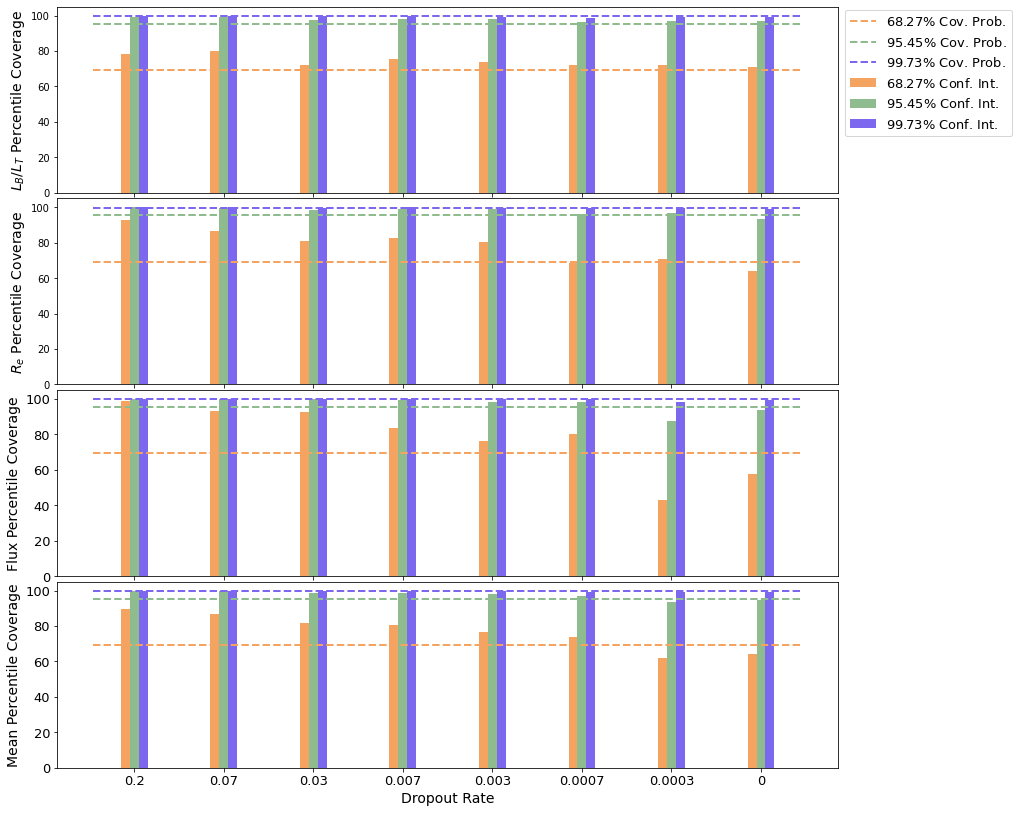
\includegraphics[width
    =\textwidth]{dropout_calibration_new.png}
    \caption{The calculated percentile coverage probabilities for different dropout rates. The top three rows show coverage probabilities for each output variable individually, while the bottom row shows the probabilities averaged over the three variables. The coverage probabilities are defined as the percentage of the total test examples where the  true  value  of  the  parameter  lies  within  a  particular confidence interval of the predicted distribution. A dropout rate of $7\times10^{-4}$ leads to coverage probabilities very close to their corresponding confidence levels.}
    \label{fig_c2:dropout_calibration}
\end{figure*}

Therefore, we first apply the logit transformation to $L_B/L_T$ and log transformations to $R_e$ and $F$: 

\begin{equation}
\boldsymbol{Y_n'} = f''(\boldsymbol{Y}_n'') = \left( \log \frac{L_B/L_T}{1 - L_B/L_T}, \log R_e, \log F \right) ,
\label{eq:transformation_f''}
\end{equation} 

\noindent
where $\boldsymbol{Y}_n'' = [{L_B/L_T,R_e,F}]$ is the set of ground-truth parameters corresponding to the simulated image, $\boldsymbol{X}_n$, and $f''$ is how we will refer to the transformation in Equation\,\ref{eq:transformation_f''}. Note that the uniformity of these transformations allows us to write the likelihood in terms of a multivariate Gaussian distribution. Next we apply the standard scaler to each parameter (calibrated on the training data), which amounts to subtracting the mean value of each parameter and scaling its variance to unity:
%This transformation, which we denote by $f'$, can be written as

\begin{equation}
\boldsymbol{Y}_n = f'(\boldsymbol{Y}_n')\,\,\,\,\,\mathrm{where}\,\,\,\,\,{Y}_{n,i} = \frac{Y'_{n,i} - \overline{Y'_{i}}}{\sqrt{\operatorname{var}(Y'_{i})} ,} 
\label{eq:transformation_f'}
\end{equation}

\noindent
where the $i$ subscript refers to each of the three parameters. Combining the above transformations, $f'$ and $f''$, ensures that all three variables have similar numerical ranges.  

Note that effectively \gampen{} is trained in the $\boldsymbol{Y}_n$ variable space, and the predictions made by \gampen{} are also in this space. Thus, post training, during inference, we need to apply the inverse of the standard scaler function, $f'^{-1}$ (with no re-tuning of the mean or variance), followed by the inverse of the logit and log transformations, $f''^{-1}$, as indicated in Figure\,\ref{fig_c2:workflow}. These final transformations also ensure that the predicted values are all within the physical ranges mentioned earlier.

We train \gampen{} by minimizing the loss function in Equation\,\ref{eq:final_loss_fn} using Stochastic Gradient Descent, wherein we estimate the gradient of the loss function using a mini-batch of training samples and update the network weights and biases accordingly. Calculation of the gradient is done using the back-propagation algorithm, and we refer an interested reader to \citet{rumelhart_88} for details.

The training process involves hyper-parameters that must be chosen: the learning rate (the step-size during gradient descent), momentum (acceleration factor used for faster convergence), strength of L2 regularization ($\lambda$ in the loss function in Eqn.\,\ref{eq:final_loss_fn}), and batch size (the number of images processed before weights and biases are updated).
To choose these hyper-parameters, we trained \gampen{} with a given set of hyper-parameters for forty epochs, then verified convergence by checking whether the value of the loss function and the mean-absolute-error on the validation set had stabilized over at least the last ten epochs. An epoch of training refers to running all of the images in the training set through the network once. We chose final hyper-parameters that resulted in the lowest value for the loss function. This resulted in the following values: Learning Rate, $5\times10^{-7}$; Momentum, 0.99; Strength of L2 regularization $\lambda=10^{-4}$, and Batch Size, 16. The grid of values we used for the hyper-parameter search is as follows:- Learning Rate - $10^{-5}$, $5 \times 10^{-5}$, $10^{-6}$, $5 \times 10^{-6}$, \ldots,  $5 \times 10^{-8}$; Momentum - 0.8, 0.9, 0.95, 0.99; $\lambda$ - $10^{-5}$,$10^{-4}$, \ldots, $10^{-2}$; Batch Size: 8, 16, 32, 64.

One of the most critical adjustable parameters is the dropout rate, as it directly affects the calculation of the epistemic uncertainties (as described in \S \ref{subsec_c2:mcd}). On average, higher dropout rates lead networks to estimate higher epistemic uncertainties. To determine the optimal value for the dropout rate, we trained variants of \gampen{} with dropout rates from 0 to 0.2, all with the same optimized values of momentum, learning rate, and batch size given above. After that, we performed inference using each model as outlined in Figure \ref{fig_c2:workflow}. 

To compare these models, we calculated the percentile coverage probabilities associated with each model, defined as the percentage of the total test examples where the true value of the parameter lies within a particular confidence interval of the predicted distribution. We calculate the coverage probabilities associated with the $68.27\%$, $95.45\%$, and $99.73\%$ central percentile confidence levels, corresponding to the $1\sigma$, $2\sigma$, and $3\sigma$ confidence levels for a normal distribution. For each distribution predicted by \gampen{}, we define the $68.27\%$ confidence interval as the region on the x-axis of the distribution that contains $68.27\%$ of the most probable values of the integrated probability distribution. In order to estimate the probability distribution function from the \gampen{} predictions (which are discrete), we use kernel density estimation, which is a non-parametric technique to estimate the probability density function of a random variable. 

We calculate the $95.45\%$ and $99.73\%$ confidence intervals of the predicted distributions in the same fashion. Finally, we calculate the percentage of test examples for which the true parameter values lie within each of these confidence intervals. An accurate and unbiased estimator should produce coverage probabilities equal to the confidence interval for which it was calculated (e.g., the coverage probability corresponding to the $68.27\%$ confidence interval should be $68.27\%$).

Figure \ref{fig_c2:dropout_calibration} shows the coverage probabilities for the three output parameters individually (top three panels), as well as the coverage probabilities averaged over the three output variables (bottom panel). As can be seen, higher values of the dropout rate lead to \gampen{} over-predicting the epistemic uncertainties, resulting in too high coverage probabilities. In contrast, extremely low values lead to \gampen{} under-predicting the epistemic uncertainties. For a dropout rate of $7\times10^{-4}$, the calculated coverage probabilities are very close to their corresponding confidence levels, resulting in accurately calibrated posteriors. The dropout rate is clearly a variational parameter of \gampen{}, and all the results shown hereafter correspond to a \gampen{} model trained with a dropout rate of $7\times10^{-4}$.

It is important to note that the inclusion of the full covariance matrix in the loss function allowed us to incorporate the relationships between the different output variables in \gampen{} predictions. This allowed us to achieve simultaneous calibration of the coverage probabilities for all three output variables. 
In contrast, using only the diagonal elements of the covariance matrix resulted in substantial disagreement, for a fixed dropout rate, among the coverage probabilities of the different parameters.
%Experiments, assuming the three output variables to be independent, did not result in simultaneous calibrated coverage probabilities. 
Additionally, when we used three different neural networks to predict each output variable, we achieved a poorer overall accuracy. Thus, using the full covariance matrix, facilitated by the linear algebraic tricks outlined in \S \ref{subsec_c2:uncertainty_implementation}, allows \gampen{} to predict accurate, calibrated posteriors.

\section{Results} \label{sec_c2:results}
After training \gampen{} and tuning its hyper-parameters on the training and validation sets, as outlined in \S \ref{sec_c2:training}, we perform inference using the testing set of 22,500 galaxies. 

\subsection{Inspecting the Predicted Posteriors} \label{subsec_c2:predicted_dists}

As outlined in Figure \ref{fig_c2:workflow} and \S \ref{subsec_c2:combining_uncertainties}, during the inference phase, we pass each image in the testing set 1000 times through \gampen{}. Note that due to our use of Monte-Carlo Dropout, each of these forward passes happens through a slightly different network because of how the technique drops out (sets to zero) randomly selected neurons according to a Bernoulli distribution. This technique allows us to effectively factor in the uncertainty about our predictive model into \gampen{} predictions. For each forward pass $t$ and for each test image $\boldsymbol{\hat{X}}_n$, \gampen{} predicts a vector of means $\boldsymbol{\hat{\mu}}_{n,t}$ and a covariance matrix $\boldsymbol{\hat{\Sigma}}_{n,t}$. These two parameters are used to define a multivariate Gaussian distribution $\mathcal{N}(\boldsymbol{\hat{\mu}}_{n,t},\boldsymbol{\hat{\Sigma}}_{n,t})$ from which we draw a sample $\boldsymbol{\hat{Y}}_{n,t}$. These are then processed through two sets of transformations ($f'^{-1}$ and $f''^{-1}$) outlined in \S \ref{sec_c2:training} resulting in the transformed prediction $\boldsymbol{\hat{Y}''}_{n,t}$. The collection of these samples for the 1000 forward passes $_{t=1}^{1000}\boldsymbol{\hat{Y}''}_{n,t}$ represents the posterior distribution predicted by \gampen{} for the test image $\boldsymbol{\hat{X}}_{n}$.

\begin{figure}[htb]
    \centering
    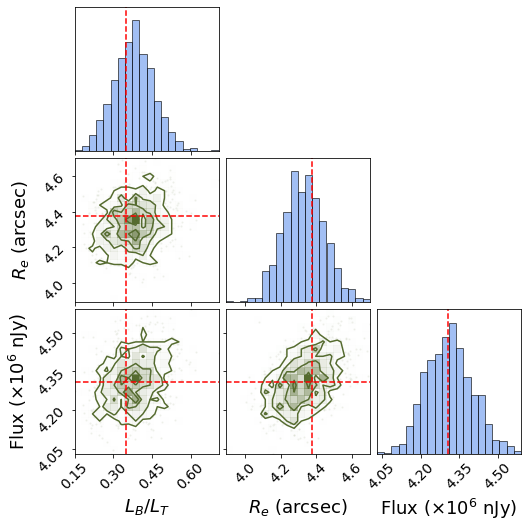
\includegraphics[width
    =0.47\textwidth]{corner.png}
    \caption{Joint and marginalized probability distributions predicted by \gampen{} for a randomly chosen galaxy in our testing set. The red dotted lines show the true values of the parameters.}
    \label{fig_c2:corner}
\end{figure}

\begin{figure*}[htb]
    \centering
    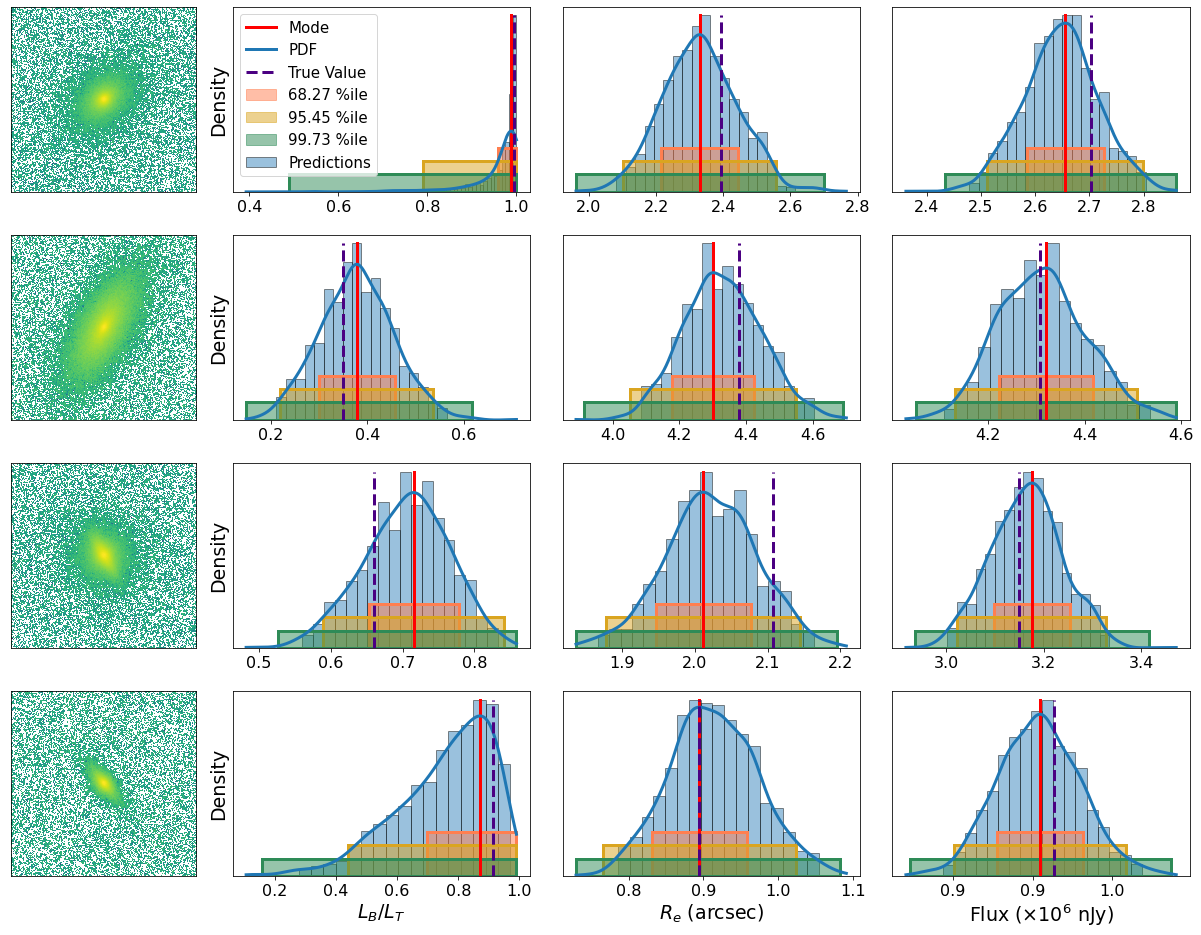
\includegraphics[width
    =\textwidth]{example_predicted_distributions_2.png}
    \caption{Examples of predicted posterior distributions for four randomly chosen simulated galaxies. The blue shaded histogram shows the predictions from \gampen\, and the blue solid lines show the associated probability distribution functions estimated by kernel density estimation. These are used to calculate the confidence intervals shown in the figure with pink, yellow, and green shading. The mode (red line) shows the most probable value of each morphological parameter. As expected, in most cases, the true value (purple line) lies within the $68.27\%$ confidence interval.}
    \label{fig_c2:example_pred_dists}
\end{figure*}

Using the above process, we extract the joint probability distribution of all the output parameters for each of the 22,500 galaxies in our test set. Figure \ref{fig_c2:corner} shows the two-dimensional joint distributions of the output parameters, as well the marginalized distributions, for a randomly chosen galaxy in our test set. 
%The red dotted lines in the figure show the true values of the parameters. 
The same galaxy %for which the joint distributions are plotted in Figure \ref{fig_c2:corner} 
is shown in the second row of Figure \ref{fig_c2:example_pred_dists},
which illustrates the predicted posterior distributions for a few more cases.
%Note that for this specific galaxy, the true values of the different parameters do lie in the densest parts of the probability density space predicted by \gampen{}. In order to show the predicted distributions for a few more cases and also to visually demonstrate the calculation of the probability density function as well as the confidence intervals, we show the marginalized histograms for a few more galaxies in Figure \ref{fig_c2:example_pred_dists}.
%In addition to the marginalized distributions, 
Figure \ref{fig_c2:example_pred_dists} also shows the image of each galaxy %in the leftmost column. 
at the left.
As expected, all the predicted distributions are unimodal, smooth, and resemble Gaussian or truncated Gaussian distributions. For each predicted distribution, the figure also shows the parameter space regions that contain $68.27\%$, $95.45\%$, and $99.73\%$ of the most probable values of the integrated probability distribution. We use kernel density estimation to estimate the probability distribution function (PDF; shown by a blue line in the figure) from the predicted values. The mode of this PDF is what we refer to as the predicted value when calculating residuals. In the figure, for most cases, the true value lies within the most probable $68.27\%$ percentile region. We also visually inspected the distributions predicted by \gampen{} for $\sim200$ galaxies to ensure that there were no systematic or catastrophic errors (e.g., substantial errors for a specific parameter only, or bi-modal or irregular distributions for specific kinds of galaxies, etc.). 

By design, \gampen{} predicts only physically possible values. This is especially apparent in the $L_B/L_T$ column of rows 1 and 4 of Figure \ref{fig_c2:example_pred_dists}. Note that to achieve this, we do not artificially truncate these distributions. Instead, we use the inverse of the logit transformation on the prediction space of \gampen{} as outlined in \S \ref{sec_c2:training}. This ensures that the predicted $L_B/L_T$ values are always between 0 and 1. Similarly, we also ensure  that the $R_e$ and $F$ values predicted by \gampen{} are positive through appropriate transformations. 

\begin{figure*}[htb]
    \centering
    \includegraphics[width
    =\textwidth]{pred_true.png}
    \caption{The true values of the galaxy parameters plotted against the most probable values predicted by \gampen{}. The black dashed line marks the $y=x$ diagonal on which perfectly recovered parameters should lie. The color of each hexagon corresponds to the number of galaxies it contains, as indicated by the colorbar at right.}
    \label{fig_c2:pred_true}
\end{figure*}

\subsection{Evaluating the Accuracy of \gampen{}} \label{subsec_c2:residuals}

In \S \ref{subsec_c2:predicted_dists}, we explored the predicted distributions for a handful of cases, where the true values of the parameters mostly lay within the densest parts of the probability distribution predicted by \gampen{}. In order to evaluate the accuracy of \gampen{}, we now report summary statistics that outline the framework's performance on the entire testing set.

\begin{table}[htbp]
    \centering
    \caption{Coverage Probabilities on the Test Set  \label{tab_c2:coverage_probs}}
    \begin{tabular}{c|ccc}
    \hline
    \hline
    Parameter & $68.27\%$ & $95.45\%$ & $99.73\%$ \\
    Name & Conf. Level & Conf. Level & Conf. Level \\
    \hline
    \hline
    $L_B/L_T$ & $71.8\%$ &  $96.9\%$ &  $98.9\%$\\
    $R_e$ &  $68.1\%$ &  $95.9\%$ &  $98.3\%$ \\
    $F$ &  $78.7\%$ &  $98.2\%$ &  $99.9\%$\\
    \hline
    Mean & $72.9\%$ &  $97.0\%$ & $99.0\%$\\
    \hline
    \multicolumn{4}{p{0.55\textwidth}}{\vskip 0.01cm \small \texttt{NOTE-} The coverage probabilities are defined as the percentage of the total test samples where the  true  value  of  the  parameter  lies  within  a particular confidence interval of the predicted distribution.}
    \end{tabular}
\end{table}

In Table \ref{tab_c2:coverage_probs}, we report the coverage probabilities that \gampen{} achieves on the test set. 
% (i.e., the percentage of test examples where the true values of the parameter lie within a particular confidence threshold of the predicted distribution, see \S\,\ref{sec_c2:training}). 
In the ideal situation, they would perfectly mirror the confidence levels; that is, $68.27\%$ of the time, the true value would lie within $68.27\%$ of the most probable volume of the predicted distribution.
(Note that in \S\,\ref{sec_c2:training} we tuned the dropout rate so they coincide over the validation set, whereas Table\,\ref{tab_c2:coverage_probs} is calculated on the testing set.) 
%Note that we tuned the dropout rate based on the coverage probabilities on the validation set in \S \ref{sec_c2:training}, whereas Table\,\ref{tab_c2:coverage_probs} is calculated on the testing set.
%Table \ref{tab_c2:coverage_probs} demonstrates that 
Clearly, \gampen{} produces well calibrated and accurate posteriors, 
%: although the coverage probabilities are not perfectly aligned for the all three parameters, they are 
consistently close to the claimed confidence levels.
%to allow the posteriors to be used for most practical purposes. 
Additionally, we note that even for the flux, for which the coverage probabilities are most discrepant, the uncertainties predicted by \gampen{} are in any case overestimates (i.e., conservative). %Thus, \gampen{} is not over-confident for any of the confidence thresholds. 
If \gampen{} were used in a scenario that requires perfect alignment of coverage probabilities, users could employ techniques such as importance sampling \citep{importance_sampling} on the distributions predicted by \gampen{}. 
%In future work, we plan to try techniques such as deep ensembles \citep{deep_ensembles} to see whether these lead to even better calibrated coverage probabilities. 

\begin{figure*}[htb]
    \centering
    \includegraphics[width
    =\textwidth]{residual_hists.png}
    \caption{Histograms of residuals for all galaxies in the testing set. We define the residuals as the difference between the true value and the most probable value predicted by \gampen{}. The dashed vertical line represents $x = 0$, denoting cases with perfectly recovered parameter values. 
    The mean ($\mu$), median ($\tilde{\mu}$), and standard deviation ($\sigma$) of each residual distribution are listed in each panel.
    %The box in the upper left corner mentions the mean ($\mu$), median ($\tilde{\mu}$), and the standard deviation ($\sigma$) of each residual distribution.
    }
    \label{fig_c2:residual_hists}
\end{figure*}

%We would like to note here again that predicting the joint posterior distribution allowed us to incorporate the structured relationship between the different output parameters within \gampen{}, allowing us to achieve simultaneous calibration of the coverage probabilities for all the three output variables. In experiments where we assumed the three output variables to be independent of each other didn't result in simultaneous calibration of coverage probabilities for all the three variables. 

Having defined the overall percentage of cases where the true values are within particular confidence levels of the predicted distributions, we now quantify the difference between the most probable values of the predicted parameters (i.e., modes of these predicted distributions) and the true values. 

Figure\,\ref{fig_c2:pred_true} shows the most probable values predicted by \gampen{} for the testing set versus the true values, %. The distribution of galaxies in this predicted v/s true space is shown 
%using a hexbin color plot, where the space is divided into 
in hexagonal bins of roughly equal size, with the number of galaxies represented according to the colorbar on the right. % side of Figure \ref{fig_c2:pred_true}. 
We have used a logarithmic colorbar to visualize even small clusters of galaxies in this plane. 
Most galaxies are clustered around the line of equality, showing that the most probable values of the distributions predicted by \gampen{} closely track the true values of the parameters. 

The middle panel of Figure\,\ref{fig_c2:pred_true} shows a small bias (note that the color scale is logarithmic) towards low predictions of $R_e$, especially for true $R_e > 4$ arcsec. Features like this have been seen before in other machine learning studies and are typically referred to as an “edge effect” -- that is, sometimes the model performs poorly at the edges of the parameter space on which it was trained. Here, since $R_e=5$ arcsec is the largest radius present in our training data, for some galaxies with $R_e$ close to 5 arcsec, the network is hesitant to predict the highest value it has ever seen and predicts a slightly lower value. This results in the small bias toward lower predicted values of $R_e$. However, note that despite this effect for a small number of galaxies; even at a  large radius, \gampen{} accurately estimates $R_e$ for the large majority of galaxies. Among some other larger deviations evident in Figure\,\ref{fig_c2:pred_true}, are predictions near the limits of $L_B/L_T$. We explore this further below. 

In Figure \ref{fig_c2:residual_hists}, we show the residual distribution for the three parameters predicted by \gampen{}. We define the residual for each parameter as the difference between the most probable predicted value and the true value, i.e., $\operatorname{Mode}(\boldsymbol{\hat{Y}_n}) - \boldsymbol{Y_n}$. The box in the upper left corner gives 
the mean ($\mu$), median ($\tilde{\mu}$), and standard deviation ($\sigma$) of each residual distribution. 
All three distributions are normally distributed (verified using the Shapiro Wilk test), and have $\mu \sim \tilde{\mu} \sim 0$.
The \gampen\ prediction of the bulge-to-total ratio is, in $\sim68.27\%$ of cases, within 0.1 of the true value.
The typical error in effective radius is $0.17$ arcsec.
Typical uncertainties in the flux are at the 0.1-1\% level.
%typical fluxes in our dataset are two-three orders of magnitude higher than these values. 
% The values of the reported standard deviations help us to understand the typical size of the errors in the values predicted by \gampen{}. For example, while predicting $L_B/L_T$, in $\sim68.27\%$ of cases, the error in the predicted value of $L_B/L_T$ is $\leq0.1$. The corresponding typical errors for $R_e$ and $F$ are $0.17$ arcsec, and $6.3\times10^4$ nJy respectively. 

Although Figures \ref{fig_c2:pred_true} and \ref{fig_c2:residual_hists} indicate the overall accuracy of \gampen{}, they do not reveal how those errors depend on location in the parameter space. This is critical information as this enables us to potentially ignore predictions for regions of parameter space that have large errors (according to the validation set).
Figure \ref{fig_c2:2d_residual_hists} shows the residuals for the three output parameters plotted against the true values. As in Figure \ref{fig_c2:pred_true}, we have split the parameter space into hexagonal bins and used a logarithmic color scale to denote the number of galaxies in each bin. The purpose of this plot is to identify regions of parameter space where \gampen{} performs especially well or badly, so that, in the future, we can flag predictions in these regions as ``very secure" or ``unreliable". Note that because we are performing the test here on simulated galaxies, we have access to the ground-truth values. However, in a scenario where \gampen{} is being used on real galaxies which have not been morphologically studied before, we won't have access to the ground-truth values, and any such cuts on the X-axis would need to be made based on the values predicted by \gampen{}. Thus, we created Figure \ref{fig_c2:2d_residual_hists_pred}, where we replaced the X-axis with the predicted values of the parameters instead of the true values. 

\begin{figure*}[htb]
    \centering
    \includegraphics[width
    =\textwidth]{2d_hist_residuals.png}
    \caption{Residuals of \gampen{} predicted parameter values plotted against the true values. The residual for each parameter is defined as the difference between the most probable predicted value and the true value, i.e., $\operatorname{Mode}(\boldsymbol{\hat{Y}_n}) - \boldsymbol{Y_n}$. The color of each hexagonal bin corresponds to the number of galaxies it contains, as shown by the colorbar on the right. The black dotted line ($y=0$) represents %the ideal scenario of 
    perfectly recovered parameters.}
    \label{fig_c2:2d_residual_hists}
\end{figure*}

\begin{figure*}[htb]
    \centering
    \includegraphics[width
    =\textwidth]{2d_hist_residuals_preds.png}
    \caption{Residuals of the output parameters plotted against the predicted values. This figure allows us to assign quality labels to \gampen{} predictions (e.g., flagging parameters that are unreliable) based on the output values. See \S\,\ref{subsec_c2:cuts} for details.}
    \label{fig_c2:2d_residual_hists_pred}
\end{figure*}

\begin{figure}[hbt]
    \centering
    \includegraphics[width
    =0.45\textwidth]{residual_hist_bt_sep.png}
    \caption{Histograms of $L_B/L_T$ residuals shown separately for single component galaxies, all double component galaxies, and double component galaxies with $0.1 < L_B/L_T < 0.85$. The standard deviation ($\sigma$) for each distribution is also shown in the top left. The dashed vertical line represents $x = 0$, denoting cases with perfectly recovered $L_B/L_T$. The apparent hard cutoffs in the distributions of the single component, and the restricted range double-component galaxies arise from the fact that the y-scale is logarithmic. We have verified that when plotted on a linear scale, the apparent hard cutoffs disappear.}
    \label{fig_c2:residual_hist_bt_sep}
\end{figure}

\begin{figure*}[htb]
    \centering
    \includegraphics[width
    =0.9\textwidth]{2d_hist_residuals_norm.png}
    \caption{Fractional residuals for the effective radius and flux plotted against their corresponding true values. Note that since we are plotting the absolute values, the ideal situation of perfectly recovered parameters is at the bottom of each panel. The right two panels show that both the residuals increase for fainter galaxies, while the top-middle panel shows that the radius residuals increase for smaller galaxies.}
    \label{fig_c2:2d_residual_hists_norm}
\end{figure*}


In both Figures \ref{fig_c2:2d_residual_hists} and \ref{fig_c2:2d_residual_hists_pred}, for most of the panels, the large majority of galaxies are clustered uniformly around the black dashed line, $y = 0$, which denotes the ideal case of perfectly recovered parameters.% with the residuals being equal to zero. 

There are a few other notable features in these two figures. In the top left panel, the $L_B/L_T$ residuals are highest near the limits of $L_B/L_T$. This is another manifestation of the edge-effect mentioned earlier, wherein sometimes machine learning algorithms perform poorly at the edges of the parameter space on which they were trained.  To delve deeper, we looked at the $L_B/L_T$ residuals separately for double and single component galaxies, as shown in Figure \ref{fig_c2:residual_hist_bt_sep}. 
For single-component galaxies, the typical $L_B/L_T$ residual ($\sigma=0.06$) is roughly half as large as for double-component galaxies ($\sigma=0.11$);
%(i.e., with both bulge and disk components). 
among the latter, the residuals are especially high when $L_B/L_T > 0.85$ or $L_B/L_T < 0.1$. In other words, accurately determining $L_B/L_T$ is challenging when both a bulge and a disk are present, and becomes even more difficult when one component strongly dominates the other. %This is not unexpected since precisely measuring the ratio of the fluxes of two galaxy components is inherently inaccurate if there are two galaxy components and one component completely dominates over the other. 
Larger residuals in the predictions near the limits of $L_B/L_T$ leads to the features seen in the top left panel of both figures.

This edge effect also results in the top and bottom streaks seen in the left panel of Figure \ref{fig_c2:pred_true}. Given the logarithmic  color bar used in this figure, note that most of the galaxies in the upper streak have true $L_B/L_T > 0.75$ and those in the bottom streak have true $L_B/L_T < 0.25$. For these cases, when one component completely dominates over the other component, precisely determining $L_B/L_T$ is challenging. For some of the galaxies with $0.25 > \mathrm{True}\,\,L_B/L_T > 0.75$, \gampen{} assigns almost the entirety of the light to the dominant component, resulting in the streaks in the left panel. We use a parameter transformation to mitigate this edge effect, as described in \S\,\ref{subsec_c2:cuts}. 

In the top-middle panels of Figures \ref{fig_c2:2d_residual_hists} and \ref{fig_c2:2d_residual_hists_pred}, there is a slight broadening of the residuals at low values of the effective radius. This result also makes sense: smaller galaxies are challenging to analyze for any image processing algorithm. Somewhat surprising features appear in the panels showing residuals of effective radius (mid-row, mid-column) and flux (bottom-row, right-column). The $R_e$ residuals increase in magnitude (with a bias towards negative values) toward increasing values of $R_e$, and the residual flux also grows rapidly with higher flux values. However, these increases are simply the result of the increasing numerical values of the parameters. To show this, Figure \ref{fig_c2:2d_residual_hists_norm} plots the dimensionless fractional $R_e$ and $F$ residuals (note that $L_B/L_T$ is inherently dimensionless), using their absolute values, such that the ideal scenario (i.e., zero residuals) is at the bottom of each panel instead of in the middle. 
In this presentation, both features noted above not only disappear but reverse.
For small values of effective radius, $R_e < 1.0$ arcsec, there is an increase in the magnitude of the residuals.
Similarly, the right two panels show that the residuals of $R_e$ and $F$ are systematically higher for faint galaxies, $F< 10^6$ nJy.% A somewhat surprising feature presents itself in the panel showing the residuals of $R_e$ v/s $R_e$ (mid-row; mid-column) and in the panel displaying residuals of the flux v/s the flux (bottom-row; right-column). The $R_e$ residuals seem to increase in magnitude (with a bias towards -ve values) at high values of $R_e$, while the residual flux also grows rapidly with higher flux values. However, it is essential to note that these increases in residuals might be trivially connected to the high numerical values of the parameters. In order to account for this, we plot the dimensionless fractional $R_e$ and $F$ residuals instead of their numerical values in Figure \ref{fig_c2:2d_residual_hists_norm} (note that $L_B/L_T$ is dimensionless inherently). Another difference is that in Figure \ref{fig_c2:2d_residual_hists_norm}, we plot the absolute values, and thus the ideal scenario (i.e., zero residuals) is at the bottom of each panel instead of being in the middle. In Figure \ref{fig_c2:2d_residual_hists_norm}, both the features noticed earlier not only disappear; but reverse. For the residuals of $R_e$ v/s $R_e$ (top row; middle column), we see that for values of $R_e < 1.0$ arcsec, there is an increase in the magnitude of the residuals. Similarly, the right two panels show that the residuals of $R_e$ and $F$ are systematically higher for galaxies fainter than $10^6$ nJy.

In other words, \gampen{} systematically becomes less accurate at predicting the radii of galaxies when their sizes become comparable to the seeing of the HSC-Wide Survey (\textit{g}-band median FWHM $\sim0.85\arcsec$). Similarly, \gampen{} finds it more challenging to predict the sizes and fluxes of fainter galaxies, just as one would expect.
%. This is in line with the fact that fainter and smaller galaxies are inherently difficult to work with using any analysis technique. 
With our previously published classification network, \gamornet{} \citep{Ghosh2020GalaxyGalaxies}, we observed a similar reduction in prediction accuracy for smaller and fainter galaxies. Figures \ref{fig_c2:2d_residual_hists}, \ref{fig_c2:2d_residual_hists_pred}, and \ref{fig_c2:2d_residual_hists_norm} help quantify the errors in \gampen{} predictions in different regions of parameter space. These will be essential in order to interpret results appropriately when applying \gampen{} to real galaxies. 
%We will also explore in \S \ref{subsec_c2:cuts} how transforming some of the predicted values can help us reduce the magnitude of the residuals. 

\vspace{0.8cm}

\subsection{Inspecting the Predicted Uncertainties} \label{subsec_c2:uncertainties}
The primary advantage of a Bayesian ML framework like \gampen{} is its ability to predict the full posterior distributions of the output parameters instead of just point estimates. Thus, we would expect such a network to inherently produce wider distributions (i.e., larger uncertainties) in regions of the parameter space where residuals are higher. Here we delineate regions of the parameter space for which \gampen{} predicts broader distributions and we see that these generally coincide with those that have the largest residuals (Figs.\,\ref{fig_c2:2d_residual_hists}, \ref{fig_c2:2d_residual_hists_pred}, \ref{fig_c2:2d_residual_hists_norm}).  

\begin{figure*}[htb]
	\centering
	\includegraphics[width
	=\textwidth]{2d_uncertainty_norm.png}
	\caption{Uncertainties predicted by \gampen{} for each parameter plotted against the true values. The $\sigma$ for each parameter is defined as the width of the $68.27\%$ confidence interval. %i.e., the parameter interval that contains $68.27\%$ of the most probable values;
	Note that we plot fractional uncertainties for radius and flux in order to make the y-axis dimensionless for all three rows.}
	\label{fig_c2:2d_uncertainty_hists_norm}
\end{figure*}

\begin{figure*}[htb]
	\centering
	\includegraphics[width
	=\textwidth]{uncer_resi.png}
	\caption{Uncertainties (widths of the $68.27\%$ confidence intervals)  predicted by \gampen{} for each parameter  versus the corresponding residuals (predicted mode minus true value). Fractional uncertainties and residuals are plotted for radius and flux in order to make all the quantities dimensionless. The trend in all three cases is that \gampen{}-estimated uncertainties increase for cases where its predictions are less accurate. The coverage probabilities reported on the test set (Table \ref{tab_c2:coverage_probs}) confirm that the predicted uncertainties are well-calibrated and correspond well to the quoted confidence intervals.}
	\label{fig_c2:uncer_resi}
\end{figure*}

Figure \ref{fig_c2:2d_uncertainty_hists_norm} shows the uncertainties for the three predicted parameters plotted against the true values of the different parameters. 
We define the uncertainty predicted for each parameter as the width of the $68.27\%$ confidence interval (i.e., the parameter interval that contains $68.27\%$ of the most probable values of the predicted distribution; see Fig.\,\ref{fig_c2:example_pred_dists}). 
The lower two panels have been normalized, so that all three panels show dimensionless fractional uncertainties.
%Note that to make the uncertainties for all three parameters dimensionless, we plot fractional uncertainties instead of numerical uncertainties .

The uncertainties in the predicted values of the radius increase sharply for galaxies with $R_e < 2$ arcsec and/or $F < 10^6$ nJy. Similarly, the uncertainties in flux increase for galaxies with $R_e < 1$ arcsec and/or $F < 10^6$ nJy. 
%Both these results show that the uncertainties predicted by \gampen{} perfectly align with our expectation that any model should be typically more uncertain in its predictions at smaller values of $R_e$ and $F$. These regions also correlate with regions where the residuals were higher, as shown in Figure \ref{fig_c2:2d_residual_hists_norm}. 
This aligns perfectly with what we expect: the sizes and fluxes of small galaxies and/or faint galaxies are not well constrained.
Just as the residuals for \gampen{} predictions were larger for small and/or faint galaxies (Figs.\,\ref{fig_c2:2d_residual_hists}, \ref{fig_c2:2d_residual_hists_pred}, \ref{fig_c2:2d_residual_hists_norm}), the uncertainties predicted by \gampen{} are also larger for these galaxies.
%compensates for the higher residuals obtained for smaller and fainter galaxies by predicting higher uncertainties in these regions. Therefore, despite having higher uncertainties in some areas of the parameter space, distributions predicted by \gampen{} are still accurate and well-calibrated, as shown in Table \ref{tab_c2:coverage_probs}.

The top left panel of Figure \ref{fig_c2:2d_uncertainty_hists_norm} shows that \gampen{} is reasonably certain of its predicted %$L_B/L_T$ values
bulge-to-total ratio across the full range of values but appears slightly more certain when $L_B/L_T \leq 0.2$ or $L_B/L_T \geq 0.8$. It turns out that the smaller uncertainties at the limits correspond to the single-component galaxies, while for the double-component galaxies, the edge effect is less pronounced, in agreement with the residuals observed in Figure \ref{fig_c2:residual_hist_bt_sep}.
%when a galaxy is completely disk dominated or bulge dominated, but is more uncertain when %$0.2 \leq L_B/L_T \leq 0.8$. 
%Therefore, \gampen{} assigns higher uncertainties to its $L_B/L_T$ predictions when there is a comparable amount of light in both the disk and bulge components. This is because such galaxies are intrinsically more challenging to classify as disk or bulge-dominated than galaxies where one component is significantly stronger than the other.
Not surprisingly, the predicted uncertainty in $R_e$ decreases with decreasing values of $L_B/L_T$ (i.e., galaxies with more dominant disks, which are on average larger than bulge-dominated galaxies in our simulation sample). 

%The top left panel of Figure \ref{fig_c2:2d_residual_hists_norm} also shows a slight trend in the same direction. We believe that this result is connected to the fact that disk-dominated galaxies have a higher maximum radius limit in our simulations, as shown in Table \ref{tab_c2:sim_para}. This causes the average radius of disk-dominated galaxies to be higher than bulge-dominated galaxies. Since the uncertainty in the predicted value of $R_e$ decreases at higher values of $R_e$, it results in disk-dominated galaxies having lower $\sigma R_e/R_e$ compared to bulge-dominated galaxies. 

In Figure \ref{fig_c2:uncer_resi}, we further assess the estimated uncertainties by investigating their relation to the measured residuals. Note that while the uncertainties represent the widths of the central $68.27\%$ confidence intervals, the residuals are the difference between the modes of the predicted distributions and the true values. Thus, we do not expect the two values to be linearly correlated; rather, on average, \gampen{} should predict larger uncertainties for galaxies with larger residuals, as is seen in all three panels of the figure. 
%Note that the streak of galaxies with extremely small $L_B/L_T$ residuals is dominated by single-components galaxies (as shown in Figure 15) for which \gampen{} correctly predicts correspondingly smaller uncertainties.
According to a Spearman's rank correlation test \citep[see][for more details]{spearman}, there is a positive correlation between the residuals and uncertainties for all three variables, and the null hypothesis of non-correlation can be rejected at extremely high significance ($p < 10^{-200}$). 
%We found the uncertainties and residuals to be positively correlated for all three variables with a correlation coefficient of 0.62, 0.46, and 0.28 for $L_B/L_T$, $R_e$, and flux respectively. This shows that for all three output variables, in general, \gampen{} produces higher uncertainties for cases where the residuals are higher -- resulting in the calibrated coverage probabilities shown in Table 2. This outlines the primary advantage of using a Bayesian framework like \gampen{} -- even in situations where the network is not perfectly accurate, it is able to predict the right level of precision, allowing its predictions to be reliable and well-calibrated.

 
The results shown in this section outline the primary advantage of using a Bayesian framework like \gampen{} -- even in situations where the network is not perfectly accurate, it is able to predict the right level of precision, allowing its predictions to be reliable and well-calibrated.

\subsection{Qualitative Transformation of \gampen{} Predictions} \label{subsec_c2:cuts}

Given that we know \gampen{} residuals are higher for certain regions of the parameter space, we explore how using only qualitative labels in those regions (instead of quantitative predictions) affects the overall residual values. The labeling is informed by the results of \S \ref{subsec_c2:residuals} and the labels are assigned by us based on the parameter values predicted by \gampen{}.
The labels are applied based on the predicted values of \gampen{} because we will not have access to true values of the parameters when applying \gampen{} to previously unanalyzed real galaxies. This is crucial given that when we apply \gampen{} to real data, techniques like this will provide us practical tools to deal with predictions in regions of the parameter-space where we know \gampen{} to be less accurate. 

\begin{figure*}[htb]
    \centering
    \includegraphics[width
    =\textwidth]{exclude_zones.png}
    \caption{The left panels show the residuals for bulge-to-total light ratio and radius plotted against their predicted values. The black dashed regions show the parameter-space where we replace the quantitative predictions with qualitative flags. Each corresponding histogram on the right shows the distribution of residuals before and after the transformation of output values.}
    \label{fig_c2:exclude_zones}
\end{figure*}

For the bulge-to-total ratio, we retain \gampen's numerical predictions for $0.1 < L_B/L_T < 0.85$, but label the more extreme galaxies as ``highly bulge-dominated" ($L_B/L_T \geq 0.85$) or ``highly disk-dominated" ($L_B/L_T \leq 0.1$).
%This is essentially saying that we are confident in \gampen{}'s exact determination of $L_B/L_T$ in the zone $0.1 < L_B/L_T < 0.85$. However, when \gampen{} predicts values  $L_B/L_T \geq 0.85$ or $\leq 0.1$, although we cannot trust the exact predicted value with a high degree of certainty, we can strongly assert that the galaxy is a strongly bulge-/disk-dominated galaxy respectively.%For $L_B/L_T$, we transform the predictions by \gampen{} such that we retain all quantitative predictions in the range $0.1 < L_B/L_T < 0.85$; but transform all values of $L_B/L_T \geq 0.85$ to a flag---``highly bulge-dominated" and all values of $L_B/L_T \leq 0.1$ to a flag---``highly disk-dominated". This is essentially saying that we are confident in \gampen{}'s exact determination of $L_B/L_T$ in the zone $0.1 < L_B/L_T < 0.85$. However, when \gampen{} predicts values  $L_B/L_T \geq 0.85$ or $\leq 0.1$, although we cannot trust the exact predicted value with a high degree of certainty, we can strongly assert that the galaxy is a strongly bulge-/disk-dominated galaxy respectively. 
The top left panel of Figure \ref{fig_c2:exclude_zones} shows the two labeled regions (black-shaded grid), which is where the residuals are highest. 
%As is evident from the figure, we choose the regions for the transformation based on the high residual values. 
The right panel of the top row shows the residual distributions including and excluding the extreme cases. As indicated by the standard deviation (top right corner), removing these extreme cases eliminates the largest errors in the predicted values of $L_B/L_T$. We also checked the accuracy of our assigned labels, and show the confusion matrix in Figure \ref{fig_c2:confusion_matrix}. From this, we calculate the net accuracy of our extreme $L_B/L_T$ labels to be $\gtrapprox99\%$. 

\begin{figure}[htb]
    \centering
    \includegraphics[width
    =0.5\textwidth]{confusion_matrix.png}
    \caption{Confusion matrix between the labels we assign when \gampen\ predicts extreme bulge-to-total ratios, $L_B/L_T <0.1$ or $>0.85$, and their true $L_B/L_T$ values. % for those galaxies. 
    The number in each block shows how many galaxies correspond to that panel, resulting in an overall accuracy $>99\%$.
    }
    \label{fig_c2:confusion_matrix}
\end{figure}

We apply similar labels to small predicted values of the effective radius. As shown in the bottom row of Figure\,\ref{fig_c2:exclude_zones}, we flag galaxies with $R_e < 1.0$ arcsec with the label ``galaxy with $R_e < 1$ arcsec" in place of the exact numerical value. %Similar to what we observed for $L_B/L_T$, the said transformation 
This reduces the typical error for $R_e$, as shown in the histogram on the right. We calculate the accuracy of this label to be $\sim97\%$.

Thus, replacing \gampen's quantitative predictions in certain small regions of the parameter space with qualitative flags results in a reduction of the typical residuals as well as highly accurate qualitative predictions.

%\subsection{Comparing \gampen{} predictions to values obtained by model fitting}
%\begin{itemize}
%    \item Description of model fitting procedure
%    \item Overall comparison of results
%    \item Conclusions you can draw from this
%\end{itemize}

%\subsection{Interpretability of the CNN?} \label{subsec_c2:interpretability}
%\begin{itemize}
%    \item Do you want to do this?
%    \item Adapt some of the results that you achieved previously for this new %regression network
%    \item Or confess that you did this for a previous classification version, but %are now releasing this. 
%\end{itemize}

\section{Discussion \& Conclusions} \label{sec:conclusions}
In this work, we introduced the Galaxy Morphology Posterior Estimation Network (\gampen{}), a machine learning framework that can estimate posterior distributions for a galaxy's bulge-to-total light ratio, effective radius, and flux. Although \gampen{} was trained to estimate these specific parameters, it can be adapted by users easily to predict other/additional morphological parameters (e.g., axis ratio, position angle, etc.). One important consideration while choosing how many parameters to predict using a single \gampen{} framework is that the number of terms in the covariance matrix will increase as $\mathcal{O}(n^2)$, where n is the number of output variables. Although the computation time will increase at a much less steep rate, the exact nature of the increase will depend on the specifics of the hardware being used.


We trained \gampen{} on two  NVIDIA Tesla P100/V100 GPUs with each training run taking about $\sim 12 - 16$ hours. \gampen{} is designed to use multiple GPUs during training and using more GPUs can reduce this training time even further. Our hyperparameter search required $\sim 30$ runs. Given that we expect $\sim 100,000$ images to always be enough to train \gampen{}, our framework can easily be trained on other datasets within a similar reasonable timescale. Once trained, it takes \gampen{} less than a millisecond to process each input galaxy image. Thus, to predict distributions ($\sim 1000$ inference runs for each image) for a million galaxies on two GPUs, \gampen{} needs $\sim 5$ days of runtime. Therefore, \gampen{} can be used to process data from future large surveys like LSST, NGRST, and Euclid within a reasonable timescale.

Training and testing \gampen{} on galaxies simulated to match Hyper Suprime-Cam Wide \textit{g}-band $z<0.25$ data, we found excellent agreement between the coverage probabilities and the corresponding confidence thresholds (Table \ref{tab_c2:coverage_probs}). 
This demonstrates that \gampen{} predicted posterior distributions are calibrated and accurate.

To account for both aleatoric and epistemic uncertainties in \gampen{} predictions, we incorporated the full covariance matrix in our loss function and used the Monte Carlo Dropout technique. Using the covariance matrix also allowed us to incorporate the structured relationships among the output parameters into \gampen{} predictions. This made it possible to achieve the simultaneous calibration of the posteriors of all three output variables (Fig. \ref{fig_c2:dropout_calibration}). In order to incorporate the covariance matrix in the loss function, we used the Cholesky decomposition and a set of linear algebraic tricks (\S \ref{subsec_c2:uncertainty_implementation}).

The typical values of errors in \gampen\ predictions are $0.10$, $0.17$ arcsec {($\sim 7\%$)}, and $6.3\times10^4$ nJy ($\sim 1\%$), for $L_B/L_T$, $R_e$, and $F$ respectively. The error in \gampen{} predictions of $R_e$ increases when $R_e < 1$ arcsec (i.e., when $R_e$ becomes comparable to the seeing of the HSC-Wide survey) and/or $F < 10^6$ nJy. Galaxies fainter than $10^6$ nJy also result in higher flux residuals. These trends result from the inherent challenge in analyzing small and faint galaxies. \gampen{} accounts for these high residuals by correctly predicting higher uncertainties in $R_e$ and $F$ for smaller and fainter galaxies. In other words, \gampen{} predicts broader distributions in regions where it is less precise.

The residuals in \gampen{} predictions of $L_B/L_T$ are high for $L_B/L_T \sim 0$ and $\sim 1$. We demonstrate that by applying qualitative labels for $0.1 \geq L_B/L_T \geq 0.85$ instead of quantitative values, we can reduce the typical error in $L_B/L_T$ to $0.076$. The produced qualitative labels (in the regions with high residuals) have extremely high accuracies of $\gtrapprox99\%$. Similarly, by labeling predictions for $R_e < 1$ arcsec, we achieve a similar reduction in the typical $R_e$ residual, and the produced labels are highly accurate. Thus, the qualitative transformation of the output values gives us tools to deal with regions of the parameter space where residuals in \gampen{} predictions are high.

It is difficult to accurately compare \gampen{}'s performance to existing morphology parameter estimation pipelines (such as GALFIT \citep{galfit}, GIM2D \citep{gim2d}, or \citet{Tuccillo2018DeepFitting}'s neural network) primarily due to the fact that none of them estimate Bayesian posteriors for the predicted parameters. GALFIT and GIM2D do include analytical estimates of errors, but \citet{haussler_07} found that both these algorithms severely underestimate the true uncertainties by an extremely large factor ($\geq 70\%$ for most galaxies). In contrast, \gampen{}'s predicted uncertainties are well-calibrated and accurate ($<5\%$ deviation). Although \gampen{}'s predictions are best used and interpreted in a probabilistic context, we compare below \gampen{}'s residuals (assuming the most probable value to be the predicted value) to the residuals achieved by other frameworks.

\citet{meert_13} used GALFIT to fit two-component light profiles to simulated Sloan Digital Sky Survey \citep[SDSS; ][]{sdss_tech_summary} galaxies and found the typical $R_e$ error to be $10\%$ and the typical magnitude error to be 0.075 mag. \gampen{} achieves a typical $R_e$ error of $\sim7\%$ and a typical magnitude error of 0.051 mag. \citet{haussler_07} used single-component fits to analyze simulated galaxies in the Hubble Space Telescope (HST) Galaxy Evolution from Morphology and SEDs \citep[GEMS; ][]{gems} survey  using GALFIT and GIM2D. They found the typical error in magnitude to be 0.05 mag using GALFIT and 0.10 mag using GIM2D. They found the typical ratio between the predicted and true $R_e$ to be $0.98\pm0.06$ using GALFIT and $1.01 \pm 0.11$ using GIM2D. The same value for \gampen{} is $0.98\pm0.08$. \citet{Tuccillo2018DeepFitting} used a CNN to obtain predictions for the parameters of a single component \sersic{} fit using simulations of HST Cosmic Assembly Near-Infrared Deep Extragalactic Legacy Survey \citep[CANDELS; ][]{candels_1} galaxies  and reported the degree of regression accuracy defined as

\begin{equation}
R^{2}=1-\frac{\sum_{i}^{n}\left(y_{i}-f_{i}\right)^{2}}{\sum_{i}^{n}\left(y_{i}-\bar{y}\right)^{2}}
\end{equation}

where $f_i$ is the predicted value of the true variable $y_i$ and $\bar{y}$ is the mean over all n samples. The $R^2$ for magnitude and $R_e$ were reported to be 0.997 and 0.972 respectively. The authors also analyzed the same galaxies using GALFIT and found the corresponding $R^2$ to be 0.983 and 0.877. The $R^2$ achieved by \gampen{} for magnitude and $R_e$ are 0.998 and 0.980 respectively. While \citet{haussler_07} and \citet{Tuccillo2018DeepFitting} did not have estimates of $L_B/L_T$ (as they used single-component fits), \citet{meert_13} did not report their residuals for $L_B/L_T$. Thus, it was not possible to compare \gampen{}'s $L_B/L_T$ residuals with these previous works. Although none of the above represent absolutely equivalent comparisons, they indicate that \gampen{}'s prediction accuracy is comparable to the most popular state-of-the-art morphology prediction tools.

\gampen{} contains a Spatial Transformer Network that enables it to crop the input image automatically. We demonstrated that \gampen{} does this based on galaxy size, without any need for specific instruction. % therein (without it being engineered to do so). 
Because the transformation is differentiable, loss gradients can be backpropagated, and thus the STN can be trained along with the rest of the framework without any additional supervision. The STN in \gampen{} will empower us to apply it to future large datasets over a broad range of redshifts without having to worry about optimal cutout sizes.  

Although in recent years there has been a significant increase in the use of CNNs for morphological determination, \gampen{} is the first machine learning framework that can robustly estimate posterior distributions of multiple morphological parameters. \gampen{} is also the first application of an STN to optical imaging in astronomy. 

By testing \gampen{} on simulated HSC \textit{g}-band galaxies, where we have access to robust ground-truth values, we demonstrated its effectiveness in recovering morphological parameters and we quantified errors/uncertainties in \gampen{} predictions across different regions of the parameter space. 

Note that, for this work, we trained and tested \gampen{} on single-band images. However, we have tested and verified that both the CNN and STN in \gampen{} can be easily adapted to intake an arbitrary number of channels, with each channel being a different band. To obtain separate morphological parameters for each band, the number of output parameters would need to be increased appropriately. We will perform a detailed evaluation of \gampen{}'s performance on multi-band images in future work.

In this work, we performed a thorough analysis of \gampen{}'s performance using HSC $z < 0.25$ simulations. However, \gampen{} can be applied to a wide variety of other datasets -- including real HSC images, imaging from other ground and space-based observatories as well as higher redshift data. However, in order to apply \gampen{} to real data, one would need to perform appropriate transfer-learning (i.e., fine-tuning the simulation trained \gampen{} models using a small amount of data from the application dataset). We refer an interested reader to \citet{Ghosh2020GalaxyGalaxies}, where we performed transfer-learning and demonstrated the application of our classification framework, \gamornet{}, to SDSS $z\sim0$ and CANDELS $z\sim1$ data.
    
Just like other image analysis methods, we expect \gampen{}'s performance to change based on the quality of the images being used (e.g., the pixel-scale of the survey, the noise, the redshift of the object). We will explore how \gampen{} performs in each of these above situations in future work.

\section*{Chapter Acknowledgments}

The authors would like to thank the anonymous referee for their insightful, encouraging, and extremely thorough comments about our manuscript.  Their constructive criticism has greatly assisted us in improving the manuscript, extending the discussion section, and making it more accessible to readers.

This material is based upon work supported by the National Science Foundation under Grant No. 1715512

CMU and AG would like to acknowledge support from the National Aeronautics and Space Administration via ADAP Grant 80NSSC18K0418. 

AG would like to acknowledge support received from the Yale Graduate School of Arts \& Sciences through the Dean's Emerging Scholars Research Award.

AG would like to acknowledge computing grants received through the Amazon Cloud Credits for Research Program and the Yale Center for Research Computing (YCRC) Resarch Credits Program. AG would also like to acknowledge computing support from YCRC and Yale Information Technology Services staff members and scientists. 

ET acknowledges support from FONDECYT Regular 1190818 and 1200495, ANID grants CATA-Basal AFB-170002, ACE210002, and FB210003, and Millennium Nucleus NCN19\_058.

The Hyper Suprime-Cam (HSC) collaboration includes the astronomical communities of Japan and Taiwan, and Princeton University. The HSC instrumentation and software were developed by the National Astronomical Observatory of Japan (NAOJ), the Kavli Institute for the Physics and Mathematics of the Universe (Kavli IPMU), the University of Tokyo, the High Energy Accelerator Research Organization (KEK), the Academia Sinica Institute for Astronomy and Astrophysics in Taiwan (ASIAA), and Princeton University. Funding was contributed by the FIRST program from Japanese Cabinet Office, the Ministry of Education, Culture, Sports, Science and Technology (MEXT), the Japan Society for the Promotion of Science (JSPS), Japan Science and Technology Agency (JST), the Toray Science Foundation, NAOJ, Kavli IPMU, KEK, ASIAA, and Princeton University. 

This paper makes use of software developed for the Large Synoptic Survey Telescope. We thank the LSST Project for making their code available as free software at  \href{http://dm.lsst.org}{http://dm.lsst.org}.

The Pan-STARRS1 Surveys (PS1) have been made possible through contributions of the Institute for Astronomy, the University of Hawaii, the Pan-STARRS Project Office, the Max-Planck Society and its participating institutes, the Max Planck Institute for Astronomy, Heidelberg and the Max Planck Institute for Extraterrestrial Physics, Garching, The Johns Hopkins University, Durham University, the University of Edinburgh, Queen’s University Belfast, the Harvard-Smithsonian Center for Astrophysics, the Las Cumbres Observatory Global Telescope Network Incorporated, the National Central University of Taiwan, the Space Telescope Science Institute, the National Aeronautics and Space Administration under Grant No. NNX08AR22G issued through the Planetary Science Division of the NASA Science Mission Directorate, the National Science Foundation under Grant No. AST-1238877, the University of Maryland, and Eotvos Lorand University (ELTE) and the Los Alamos National Laboratory.

Based, in part, on data collected at the Subaru Telescope and retrieved from the HSC data archive system, which is operated by Subaru Telescope and Astronomy Data Center at National Astronomical Observatory of Japan.



\begin{subappendices}
    
\chapter*{GaMPEN Appendix}\label{ch:gampen_appendix}

\section{Data Access}\label{sec_c2:ap:data_access}
The public data release for \gampen{} is hosted at the following two locations:

\begin{itemize}
    \item \href{http://www.ghosharitra.com/}{http://www.ghosharitra.com/}
    \item \href{http://www.astro.yale.edu/aghosh/}{http://www.astro.yale.edu/aghosh/}
\end{itemize}


\section{Extended Derivation for Bayesian Implementation of \gampen{}} \label{sec_c2:ap:mcd_deri}

In variational inference, the posterior, $p(\boldsymbol{\omega} \mid \mathcal{D})$ in Equation \ref{eq_c2:out_y_pred}, is replaced by an approximate variational distribution with an analytic form $q(\boldsymbol{\omega})$. Now, Equation \ref{eq_c2:out_y_pred} can be written as

\begin{equation}
p(\boldsymbol{\hat{Y}} \mid \boldsymbol{\hat{X}}) \approx \int p(\boldsymbol{\hat{Y}} \mid \boldsymbol{\hat{X}}, \boldsymbol{\omega}) q(\boldsymbol{\omega}) d \boldsymbol{\omega} .
\label{eq_c2:out_y_pred_vi}
\end{equation}

The choice of the variational distribution is arbitrary. 
One such choice, introduced by \cite{gal_2016}, involves dropping different neurons from some layers in order to assess the impact on the model. 
The dropout technique was introduced by \cite{Srivastava2014Dropout:Overfitting} in order to prevent neural networks from overfitting; they temporarily removed random neurons from the network according to a Bernoulli distribution, i.e., individual nodes were set to zero with a probability, $p$, known as the dropout rate. 

In the variational application, we use dropouts to interrogate the model. 
Specifically, 
if $p_{i}$ is the probability of a neuron being turned off, and
$\left[z_{i, j}\right]_{j=1}^{J_{i-1}}$ is a vector of length $J_{i-1}$ containing the Bernoulli-distributed random variables for unit $j=1, \ldots, J_{i-1}$ in the $(i-1)^{th}$ layer with probabilities $p_i$, then

\begin{equation}
%\begin{aligned}
\boldsymbol{\omega}_{i} =\boldsymbol{M}_{i} \cdot \operatorname{diag}\left(\left[z_{i, j}\right]_{j=1}^{J_{i-1}}\right) ,
%\end{aligned}
\label{eq_c2:bernoulli}
\end{equation}

\noindent
where $\boldsymbol{M}_i$ is the $J_i \times J_{i-1}$ matrix of variational parameters to be optimized. 

Thus, sampling from $q(\boldsymbol{\omega})$ is now equivalent to using dropouts on a set of layers, with weights $\boldsymbol{M}$ %corresponding to each 
(i.e., $\boldsymbol{M}_i$ for the $i^{th}$ layer). 
We perform inference on the trained network by 
% Once the network has been trained, we can perform inference by 
approximating Equation \ref{eq_c2:out_y_pred_vi} with a Monte Carlo integration: 

\begin{equation}
\int p(\boldsymbol{\hat{Y}} \mid \boldsymbol{\hat{X}}, \boldsymbol{\omega}) q(\boldsymbol{\omega}) d \boldsymbol{\omega} \approx \frac{1}{T} \sum_{t=1}^{T} p(\boldsymbol{\hat{Y}} \mid \boldsymbol{\hat{X}}, \boldsymbol{\omega}_t) ,
\end{equation}

\noindent
wherein we perform $T$ forward passes with dropout enabled and $\boldsymbol{\omega}_t$ is the set of weights during the $t$\textsuperscript{th} forward pass.

\section{Extended Derivation of the Loss Function} \label{sec_c2:ap:final_loss_deri}


As outlined in Equation \ref{eq_c2:out_y_pred}, we seek the most likely set of model parameters given our training data, %$\mathcal{D}$, 
i.e., we maximize 

\begin{equation}
p(\boldsymbol{\omega} \mid \mathcal{D}) \propto p(\mathcal{D} \mid \boldsymbol{\omega})p(\boldsymbol{\omega}) .
\label{eq_c2:bayes_rule}
\end{equation}

In Equation\,\ref{eq_c2:bayes_rule}, $p(\boldsymbol{\omega})$ is the prior on the neural networks weights -- which, for our case, happens to be Gaussian. Besides the weight prior, what also matters is the prior induced on the output parameters of \gampen{}. And as outlined above, we use a multivariate Gaussian prior for the output. Please refer to \cite{wilson_20} for a detained discussion on priors in Bayesian deep learning. 

\sloppy For a regression task using a standard CNN, wherein the network outputs predictions  $\hat{\boldsymbol{Y}}_{n}\left(\boldsymbol{\hat{X}}_{n}, \boldsymbol{\omega}\right)$ for true values $\boldsymbol{Y}_{n}$ , one popular choice is to minimize the squared-error loss function $\sum_{n} \left\|\boldsymbol{Y}_n-\boldsymbol{\hat{Y}}_n\left(\boldsymbol{\hat{X}}_n, \boldsymbol{\omega}\right)\right\|^{2}$, where the sum over $n$ denotes a sum over the training set. However, in contrast to the traditional approach, for each new test image $\boldsymbol{\hat{X}}$, \gampen{} needs to predict the parameters of a multivariate Gaussian distribution, $\mathcal{N}(\boldsymbol{\mu}, \boldsymbol{\Sigma})$. 

Now, as discussed in \S \ref{subsec_c2:mcd}, we replace $p(\boldsymbol{\omega} \mid \mathcal{D})$ in Equation \ref{eq_c2:out_y_pred} with an approximating variational distribution $q(\boldsymbol{\omega})$. This is performed by minimizing their Kullback-Leibler (KL) divergence, a measure of the similarity between two distributions. Since minimizing the KL divergence is equivalent to maximizing the log-evidence lower bound,

\begin{equation}
\log \mathcal{L}_{\mathrm{VI}}= \int q(\omega) \log p( \left\{\boldsymbol{Y}_{n=1}^{N}\right\} \mid \left\{\boldsymbol{X}_{n=1}^N\right\}, \boldsymbol{\omega}) d \boldsymbol{\omega}  - \mathrm{KL}(q(\omega) \| p(\omega)) .
\label{eq_c2:log_likelihood_vi}
\end{equation}

\noindent
The first term in Equation \ref{eq_c2:log_likelihood_vi} is the log-likelihood for the output parameters for the training set, and as shown in \cite{gal_2016}, the KL term can be approximated as an $L_2$ regularization. Therefore, Equation \ref{eq_c2:log_likelihood_vi} can be written as 

\begin{equation}
\log \mathcal{L}_{\mathrm{VI}} \sim \sum_{n=1}^{N} \log \mathcal{L}\left(\boldsymbol{Y}_{n}, \boldsymbol{\hat{Y}}_{n}\left(\boldsymbol{X}_{n}, \boldsymbol{\omega}\right)\right)-\lambda \sum_{i}\left\|\boldsymbol{\omega_{i}}\right\|^{2} ,
\label{eq_c2:log_likelihood_vi_2}
\end{equation}

\noindent
where $\log \mathcal{L}\left(\boldsymbol{Y}_{n}, \boldsymbol{\hat{Y}}_{n}\left(\boldsymbol{X}_{n}, \boldsymbol{\omega}\right)\right)$ is the log-likelihood of the network predictions $\boldsymbol{\hat{Y}}_{n}\left(\boldsymbol{X}_{n}, \boldsymbol{\omega}\right)$ for training input $\boldsymbol{X}_n$ with true values $\boldsymbol{Y}_n$, $\lambda$ is the strength of the regularization term, and $\boldsymbol{\omega}_i$ are sampled from $q(\boldsymbol{\omega})$. 

For the multivariate Gaussian distribution predicted by \gampen{}, $\mathcal{N}(\boldsymbol{\mu}, \boldsymbol{\Sigma})$, we can write the log-likelihood of the network predictions (first-term on the right side in Equation \ref{eq_c2:log_likelihood_vi_2}) as 

\begin{equation}
\log \mathcal{L} \propto  \sum_{n}  -\frac{1}{2}\left[\boldsymbol{Y}_{n}-\boldsymbol{\hat{\mu}}_{n}\right]^{\top} \boldsymbol{\hat{\Sigma}}_n^{-1}\left[\boldsymbol{Y}_{n}-\boldsymbol{\hat{\mu}}_{n}\right] -\frac{1}{2} \log [\operatorname{det}(\boldsymbol{\hat{\Sigma}}_n)] ,
\label{eq_c2:effective_log_likelihood}
\end{equation}

\noindent
where $\boldsymbol{\hat{\mu}}_n$ and $\boldsymbol{\hat{\Sigma}}_n$ are the mean and covariance matrix of the multivariate Gaussian distribution predicted by \gampen{} for an image, $\boldsymbol{X}_n$. 

We train \gampen{} by minimizing the negative log-likelihood of the output parameters for the training set, which by combining Eqs. \ref{eq_c2:log_likelihood_vi_2} and \ref{eq_c2:effective_log_likelihood}, can be written as

\begin{equation}
- \log \mathcal{L}_{VI} \propto  \sum_{n} \frac{1}{2}\left[\boldsymbol{Y}_{n}-\boldsymbol{\hat{\mu}}_{n}\right]^{\top} \boldsymbol{\hat{\Sigma_n}}^{-1}\left[\boldsymbol{Y}_{n}-\boldsymbol{\hat{\mu}}_{n}\right] + \frac{1}{2} \log [\operatorname{det}(\boldsymbol{\hat{\Sigma_n}})] + \lambda \sum_{i}\left\|\boldsymbol{\omega_{i}}\right\|^{2} .
\label{eq_c2:ap:final_loss_fn}
\end{equation}

\section{Additional Technical Details on \gampen{}}

In Table \ref{tab_c2:network_layers}, we have outlined the various layers of the \gampen{} framework along with the important parameters of each layer and the corresponding activation functions.


\begin{longtable}{cccc}
    \caption{Structure of GaMPEN}\\
    \label{tab_c2:network_layers}\\
    \hline
    \hline
    Order & Type of Layer & Layer Description & Activation Function \\
    \hline
    \hline
    \multicolumn{4}{c}{Upstream Spatial Transformer Network} \\
        \hline 
        \hline
        1 & Input & Size: $239\times239$ & --  \\
        %\hline
        2 & Convolutional & Filters: 64 $\vert$ Size: 11 & ReLU\textsuperscript{a} \\
        %\hline   
        3 & Max-Pooling & Kernel Size: 3 $\vert$ Strides: 2 & -- \\
        %\hline
        4 & Convolutional & Filters: 96 $\vert$ Size: 9 & ReLU \\
        %\hline
        5 & Max-Pooling & Kernel Size: 3 $\vert$ Strides: 2 & -- \\
        %\hline
        6 & Fully Connected & No. of neurons: 32 & ReLU \\
        %\hline
        7 & Fully Connected & No. of neurons: 1 & Linear \\
        %\hline
        & & & \\
        \hline
        \hline
        \multicolumn{4}{c}{Downstream Morphological Estimation Network} \\
        \hline
        \hline
        1 & Input & Size: $239\times239$ & --  \\
        2 & Convolutional & Filters: 64 $\vert$ Size: 3 $\vert$ Strides: 1 & ReLU \\
        3 & Dropout & - & - \\
        4 & Convolutional & Filters: 64 $\vert$ Size: 3 $\vert$ Strides: 1 & ReLU \\
        5 & Max-Pooling & Kernel Size: 2 $\vert$ Strides: 2 & -- \\
        6 & Dropout & - & - \\
        7 & Convolutional & Filters: 128 $\vert$ Size: 3 $\vert$ Strides: 1 & ReLU \\
        8 & Dropout & - & - \\
        9 & Convolutional & Filters: 128 $\vert$ Size: 3 $\vert$ Strides: 1 & ReLU \\
        10 & Max-Pooling & Kernel Size: 2 $\vert$ Strides: 2 & -- \\
        11 & Dropout & - & - \\
        12 & Convolutional & Filters: 256 $\vert$ Size: 3 $\vert$ Strides: 1 & ReLU \\
        13 & Dropout & - & - \\
        14 & Convolutional & Filters: 256 $\vert$ Size: 3 $\vert$ Strides: 1 & ReLU \\
        15 & Dropout & - & - \\
        16 & Convolutional & Filters: 256 $\vert$ Size: 3 $\vert$ Strides: 1 & ReLU \\
        17 & Max-Pooling & Kernel Size: 2 $\vert$ Strides: 2 & -- \\
        18 & Dropout & - & - \\
        19 & Convolutional & Filters: 512 $\vert$ Size: 3 $\vert$ Strides: 1 & ReLU \\
        20 & Dropout & - & - \\
        21 & Convolutional & Filters: 512 $\vert$ Size: 3 $\vert$ Strides: 1 & ReLU \\
        22 & Dropout & - & - \\
        23 & Convolutional & Filters: 512 $\vert$ Size: 3 $\vert$ Strides: 1 & ReLU \\
        24 & Max-Pooling & Kernel Size: 2 $\vert$ Strides: 2 & -- \\
        25 & Dropout & - & - \\
        26 & Convolutional & Filters: 512 $\vert$ Size: 3 $\vert$ Strides: 1 & ReLU \\
        27 & Dropout & - & - \\
        28 & Convolutional & Filters: 512 $\vert$ Size: 3 $\vert$ Strides: 1 & ReLU \\
        29 & Dropout & - & - \\
        30 & Convolutional & Filters: 512 $\vert$ Size: 3 $\vert$ Strides: 1 & ReLU \\
        31 & Max-Pooling & Kernel Size: 2 $\vert$ Strides: 2 & -- \\
        32 & Fully Connected & No. of neurons: 4096 & ReLU \\
        33 & Dropout & - & - \\
        34 & Fully Connected & No. of neurons: 4096 & ReLU \\
        35 & Dropout & - & - \\
        36 & Fully Connected & No. of neurons: 9 & Linear \\
        \hline 
        \multicolumn{4}{p{0.95\textwidth}}{\vspace{0.01cm} \small \textsuperscript{a} Rectified Linear Unit} \\
        \multicolumn{4}{p{0.95\textwidth}}{\small \texttt{NOTE-} The dropout rate of the various layers are set according to the calibration step described in \S \ref{sec_c2:training}} \\
\end{longtable}

\end{subappendices}
\chapter{Morphological Parameters and Associated Uncertainties for 8 Million Galaxies in the Hyper Suprime-Cam Wide Survey} \label{chap:hsc_morph}

Adapted from the version available on arXiv: \href{https://arxiv.org/abs/2212.00051}{2212.00051} | Accepted for publication by the American Astronomical Society in \textit{The Astrophysical Journal (in press)} \\
{\large \emph{Aritra Ghosh, C. Megan Urry, Aayush Mishra, Laurence Perreault-Levasseur, Priyamvada Nataranjan, David B. Sanders, Daisuke Nagai, Chuan Tian, Nico Cappelluti, Jeyhan S. Kartaltepe, Meredith C. Powell, Amrit Rau, and Ezequiel Treister}}\\


We use the Galaxy Morphology Posterior Estimation Network (GaMPEN) to estimate morphological parameters and associated uncertainties for $\sim 8$ million galaxies in the Hyper Suprime-Cam (HSC) Wide survey with $z \leq 0.75$ and $m \leq 23$. GaMPEN is a machine learning framework that estimates Bayesian posteriors for a galaxy's bulge-to-total light ratio ($L_B/L_T$), effective radius ($R_e$), and flux ($F$). By first training on simulations of galaxies and then applying transfer learning using real data, we trained GaMPEN with $<1\%$ of our data-set. This two-step process will be critical for applying machine learning algorithms to future large imaging surveys, such as the Rubin-Legacy 
Survey of Space and Time (LSST), the Nancy Grace Roman Space Telescope (NGRST), and Euclid. By comparing our results to those obtained using light-profile fitting, we demonstrate that GaMPEN's predicted posterior distributions are well-calibrated ($\lesssim 5\%$ deviation) and accurate. This represents a significant improvement over light profile fitting algorithms which underestimate uncertainties by as much as $\sim60\%$. For an overlapping sub-sample, we also compare the derived morphological parameters with values in two external catalogs and find that the results agree within the limits of uncertainties predicted by GaMPEN. This step also permits us to define an empirical relationship between the S\'ersic index and $L_B/L_T$ that can be used to convert between these two parameters. The catalog presented here represents a significant improvement in size ($\sim10 \times $), depth ($\sim4$ magnitudes), and uncertainty quantification over previous state-of-the-art bulge+disk decomposition catalogs. With this work, we also release GaMPEN's source code and trained models, which can be adapted to other data sets.


\section{Introduction} \label{sec_c3:intro}

The morphology of galaxies has been shown to be related to various other fundamental properties of galaxies and their environment, including galaxy mass, star formation rate, stellar kinematics, merger history, cosmic environment, and the influence of supermassive black holes \citep[e.g.,][]{Bender1992DynamicallyProperties,Tremaine2002TheCorrelation,pozzetti_10, wuyts_11, Huertas-Company2016MassCANDELS,powell_17, hsc_morph_den, Dimauro2022CoincidenceGrowth}. Therefore, quantitative measures of the morphological parameters for large samples of galaxies at different redshifts are of fundamental importance in understanding the physics of galaxy formation and evolution. 

Distributions of morphological quantities alone can place powerful constraints on possible galaxy formation scenarios. And when combined with other physical quantities, they can provide key insights into evolutionary processes at play or even reveal the role of new physical  mechanisms that impact evolution \citep[e.g.,][]{Kauffmann2004TheGalaxies,Weinmann2006PropertiesMass,Schawinski2007TheGalaxies,vanderWel2008TheMass,Schawinski2014TheGalaxies}. However, such studies often involve subtle correlations or hidden variables within strong correlations that demand greater statistics and measurement precision than what has been available in the preceding decades. %Traditionally, an 
An often-overlooked factor in such studies has been the computation of robust uncertainties. The computation of full Bayesian posteriors for different morphological parameters is crucial for drawing scientific inferences that account for uncertainty and, thus are indispensable in 
the derivation of robust scaling relations  \citep[e.g.,][]{Bernardi2013TheProfile, vanderWel20143D-HST+CANDELS:3} or tests of theoretical models using morphology \citep[e.g.,][]{Schawinski2014TheGalaxies}.

A quantitative description of galaxy morphology is typically expressed in terms of its structural parameters --- brightness, shape, and size --- all of which can be determined by fitting a single two dimensional analytic light profile to the galaxy image \citep[e.g.,][]{vdw_12,tarsitano_18}. However, moving beyond single-component determinations by using separate components to analyze galaxy sub-structure (e.g., disk, bulge, bar, etc.) can provide us additional insights into the formation mechanisms of these components: bulges, disks, and bars may be formed as a result of secular evolution \citep[e.g.,][]{kormendy_1979,kormendy_2004, genzel_2008, sellwood_2014} or due to the interaction of disk instabilities with smooth and clumpy cold streams \citep[e.g.,][]{dekel_09a,dekel_09b}. In this sense, contrary to what is often expected, bulges can also be formed without major galaxy mergers. 

Over the last decade, machine learning (ML) has been increasingly used for a wide variety of tasks---from identifying exoplanets to studying black holes \citep[e.g.,][]{ml_pz,ml_sz,Shallue2018IdentifyingKepler-90,Sharma2020ApplicationClassification,Natarajan2021QuasarNet:Holes}. Unsurprisingly, these algorithms have become increasingly popular for determining galaxy morphology as well. \citep[e.g.,][]{Dieleman2015Rotation-invariantPrediction, Huertas-Company2015ALEARNING, Tuccillo2018DeepFitting, gamornet_paper, Hausen2020MorpheusData, Walmsley2020GalaxyLearning, Cheng2021GalaxyNetworks, Vega-Ferrero2021PushingSurvey, Tarsitano2022ImageLearning}. The use of these techniques has been driven by the fact that  traditional methods of analyzing morphologies---visual classification and template fitting---are not scalable to the data volume expected from future surveys such as the Vera Rubin Observatory Legacy Survey of Space and Time \citep[LSST;][]{lsst}, the Nancy Grace Roman Space Telescope \citep[NGRST;][]{ngrst}, and Euclid \citep{euclid}. 

Most previous applications of ML to galaxy morphology produced broad, qualitative classifications rather than numerical estimates of morphological parameters. \citet{Tuccillo2018DeepFitting} did estimate parameters of single-component \sersic{} fits. However, they did not analyze galaxy sub-structures or provide uncertainties. In order to address these challenges, in Chapter \ref{ch:gampen}, we introduced The Galaxy Morphology Posterior Estimation Network (\gampen{}). \gampen{} is a machine learning framework that estimates full Bayesian posteriors for a galaxy's bulge-to-total light ratio ($L_B/L_T$), effective radius ($R_e$), and flux ($F$). \gampen{} takes into account covariances between the different parameters in its predictions and has been shown to produce calibrated, accurate posteriors. 

\gampen{} can also automatically crop input galaxy cutouts to an optimal size before determining their morphology. This feature is critical given that morphology-determination ML frameworks typically require input cutouts of a fixed size, and thus, cutouts of a ``typical" size often contain secondary objects in the frame. By cropping out most secondary objects in the frame, \gampen{} can make more accurate predictions over wide ranges of redshift and magnitude. 

\begin{figure}[htb]
    \centering
    \includegraphics[width = 0.65\textwidth]{hsc_depth.png}
    \caption{The limiting absolute magnitudes probed by the Hyper Suprime-Cam (HSC) Wide Survey and Sloan Digital Sky Survey (SDSS) at different redshifts.}
    \label{fig_c3:hsc_depth}
\end{figure}

In this chapter, we use \gampen{} to estimate Bayesian posteriors for $L_B/L_T$, $R_e$, and $F$ for $\sim 8$ million galaxies with $z \leq 0.75$ from the Hyper Suprime-Cam (HSC) Wide survey \citep{hsc_design}. A few recent works have studied the morphology of smaller subsets of HSC galaxies: \citet{hsc_morph_den} classified $\sim2\times10^5$ massive HSC galaxies into spiral and non-spiral galaxies, while \citet{hsc_mass_size} analyzed $\sim1.5\times10^6$ HSC galaxies using single-component \sersic{} fits. To date, the state-of-the-art morphological catalog that provided bulge+disk decomposition parameters at low redshift has been that of \citet{simard_11}, which used Sloan Digital Sky Survey \citep[SDSS; ][]{sdss_tech_summary} imaging to estimate morphological parameters of $\sim1$ million $m < 18$ galaxies, most with $z < 0.2$. As Figure \ref{fig_c3:hsc_depth} shows, HSC imaging allows us to probe much fainter magnitudes than SDSS with significantly better seeing (0.\arcsec85 for HSC-W \gb{} compared to 1.\arcsec4 for SDSS \gb{}). The catalog presented in this paper builds on \citet{simard_11} by providing an order of magnitude increase in sample size and probing four magnitudes deeper, to a higher redshift threshold. Along with estimates of parameters, this catalog also estimates robust uncertainties of the predicated parameters, which have typically been absent from previous large morphological catalogs. This catalog represents a significant step forward in our capability to quantify the shapes and sizes of galaxies in our universe. 


This paper also demonstrates that ML techniques can be used to study morphology in new surveys, which do not have already-classified large training sets available. Most previous works involving ML to study galaxy morphology have depended on the availability of an extensive training set of real galaxies with known properties from the same survey or a similar one. However, if Convolutional Neural Networks (CNNs) are to replace traditional methods for morphological analysis, we must be able to use them on new surveys that do not have a morphological catalog readily available to be used as a training set. In this paper, we demonstrate that by first training on simulations of galaxies and then using real data for transfer learning (fine-tuning the simulation-trained network), we can fully train \gampen{}, while having to label $<1\%$ of our dataset. This work outlines an easy pathway to apply morphological ML techniques to upcoming large imaging surveys.  

In \S \ref{sec_c3:data}, we describe the HSC data used in this study, along with the simulated two-dimensional light profiles. \S \ref{sec_c3:method} provides a description of how we train \gampen{}. In \S \ref{sec_c3:galfitting}, we outline how we determined the morphological parameters of $\sim60,000$ HSC-Wide galaxies for transfer learning and validating the results of our ML framework. \S \ref{sec_c3:results} provides detailed information on the accuracy of \gampen{}'s predictions. \S \ref{sec_c3:compare} compares our predictions to that of other catalogs. We end with a summary and discussion of our results in \S \ref{sec_c3:conclusions}.

The full Bayesian posteriors for all $\sim 8$ million galaxies are being released with the publication of this work. We are also releasing the source code of \gampen{}, along with the trained models and extensive documentation and tutorials on how to use \gampen{}. The public data release is described in Appendix \ref{sec_c3:ap:data_access}.

\section{Data} \label{sec_c3:data}

\subsection{Hyper Suprime-Cam Data} \label{sec_c3:hsc_data}

We apply \gampen{} to \textit{g},\textit{r},\textit{i}-band data from the Hyper Suprime-Cam (HSC) Subaru Strategic Program Public Data Release 2 \citep[PDR2;][]{hsc_pdr2}. The Subaru Strategic Program, ongoing since 2014, uses the HSC prime-focus camera, which provides extremely high sensitivity and resolving power due to the large 8.2 meter mirror of the Subaru Telescope. 
\begin{figure}[htb]
    \centering
    \includegraphics[width = 0.65\textwidth]{data_lambda.png}
    \caption{
    The filter used for each redshift bin is shown along with the wavelength range sampled by each filter. The blue line shows where rest-frame $450$ nm emission falls for redshifts labeled on the x-axis. As this figure shows, the chosen filters allow us to consistently perform morphology determination in the rest-frame \gb{}-band.}
    % The effective response curves of the broad-band HSC filters are shown along with the observed wavelength at different redshifts for emission at a rest-frame wavelength of $450$ $nm$. The upper x-axis shows the throughput of the different filters, and the bottom x-axis shows the redshift. The shaded regions demarcate the filter used for each redshift bin in order to consistently perform morphology determination in the rest-frame \gb{}-band.}
    %Effective response curves of the broad-band HSC filters, with throughput labeled on the upper x-axis. The blue line shows where rest-frame $450$ nm emission falls for redshifts labeled on the lower x-axis. Shaded regions indicate the filter analyzed for each redshift bin in order to consistently perform morphology determination in the rest-frame \gb{}-band.}
    \label{fig_c3:hsc_response}
\end{figure}

In order to have a large but uniform sample of HSC PDR2 galaxies, we focus on the largest volume HSC survey, namely, the Wide layer, which covers $1400$ deg$^2$ to the nominal survey depth in all filters and contains over 450 million primary objects. To consistently perform morphology determination in the rest-frame \gb-band across our entire sample, we use different filters for galaxies at different redshifts, as shown in Figure \ref{fig_c3:hsc_response}. We use \gb-band for $z\leq0.25$, \rb-band for $0.25<z\leq0.50$, and \ib-band for $0.50<z\leq0.75$. Given HSC's typical seeing, all objects with sizes $\lesssim5$\, kpc cannot be resolved beyond $z=0.75$. Therefore, given that the HSC-Wide light profiles of the large majority of galaxies beyond this redshift will be dominated by the PSF, we restrict this work till $z=0.75$ and will explore the application of \gampen{} to higher redshift deeper HSC data in future work. 

In order to select galaxies, we used the PDR2 galaxy catalog produced using forced photometry on coadded images. The HSC data has been reduced using a pipeline built on the prototype pipeline developed by the Rubin Observatory's Large Synoptic Survey Telescope's Data Management system, and we refer the interested reader to \citet{hsc_pipeline} for more details. We use the \texttt{extendedness\_value} flag only to select extended sources. The \texttt{extendedness\_value} flag relies on the difference between the Composite Model (CModel) and PSF magnitudes to separate galaxies from stars, and contamination (from stars) increases sharply for $m > 23$ for median HSC seeing in the Wide layer as outlined \href{https://hsc-release.mtk.nao.ac.jp/doc/index.php/stargalaxy-separation-2/}{here}\footnote{\href{https://hsc-release.mtk.nao.ac.jp/doc/index.php/stargalaxy-separation-2/}{https://hsc-release.mtk.nao.ac.jp/doc/index.php/stargalaxy-separation-2/}}. Thus, for each redshift bin, we  select galaxies with magnitude $m < 23$ (in the appropriate band). The full query to download the data in each redshift bin is available in Appendix \ref{ap:data}.

\begin{table}[htbp]
\centering
\caption{Data Characteristics  \label{tab_c3:data}}
\begin{tabular}{ccccc}
\hline
\hline
Sample & Redshift & Number & Imaging & Spectra \\
\hline
    \hline
    Low-z & $z\leq0.25$ & 820,566 & \gb{} & 7.4\% \\
    Mid-z & $0.25 < z\leq0.50$ & 2,937,871 & \rb{} & 2.4\% \\
    High-z & $0.50 < z\leq0.75$ & 4,247,208 & \ib{} & 1.6\% \\
\hline
\end{tabular}
\end{table}

\begin{figure}[htb]
    \centering
    \includegraphics[width = 0.95\textwidth]{z_mag_distr_old.png}
    \caption{Redshift ({\it left}) and magnitude ({\it right}) distributions for the $\sim8$ million galaxies used in this study.
    We used spectroscopic redshifts when available and high-quality photometric redshifts otherwise. The spectroscopic completeness
    of each sub-sample is shown in Table \ref{tab_c3:data}.}
    \label{fig_c3:z_mag_distr}
\end{figure}

We use spectroscopic redshifts when available ($\sim 2.5\%$) and high-quality photometric redshifts otherwise. The spectroscopic redshifts were collated by the HSC Subaru Strategic Program (SSP) team from a wide collection of spectroscopic surveys -- zCOSMOS DR3 \citep{lilly_09}, UDSz \citep{bradshaw_13}, 3D-HST \citep{momcheva_16}, FMOS-COSMOS \citep{silverman_15}, VVDS \citep{lefevre_13}, VIPERS PDR1 \citep{garilli_14}, SDSS DR12 \citep{alam_15}, GAMA DR2 \citep{liske_15}, WiggleZ DR1 \citep{drinkwater_10}, DEEP2 DR4 \citep{newman_13}, PRIMUS DR1 \citep{cool_13}, and VANDELS DR2 \citep{vandels}. The photometric redshifts in HSC PDR2 were calibrated based on the above spectroscopic sample and were calculated using the Direct Empirical Photometric code (DEmP; \citeauthor{demp} \citeyear{demp}), an empirical
quadratic polynomial photometric redshift fitting code, and Mizuki \citep{mizuki}, a Bayesian template fitting code. For an extended description, we refer the interested reader to \citet{photoz_hsc_pdr2}. To remove galaxies with unsecure photometric redshifts, we set the \texttt{photoz\_risk\_best} parameter $<0.1$, which controls the risk of the photometric redshift being outside the range $z_{\mathrm{true}} \pm 0.15(1+z_{\mathrm{true}})$, with 0 being extremely safe to 1 being extremely risky. Using the \texttt{cleanflags\_any} flag, we further excluded objects flagged to have any significant imaging issues (in the relevant band) by the HSC pipeline. This flag can be triggered by a wide range of issues; however, for $\sim 80\%$ of cases, the flag was triggered by cosmic ray hits, as shown in Appendix \ref{ap:data}. We checked and confirmed that none of the above cuts significantly modified the redshift or magnitude distribution of our galaxy sample. 

\begin{figure*}[htb]
    \centering
    \includegraphics[width = 0.95\textwidth]{real_data_examples.png}
    \caption{Four randomly chosen galaxy cutouts are shown here for each redshift bin, with the object of interest at the center of each cutout. Note that most of these cutouts have secondary objects in the frame, which can often cause ML algorithms to produce spurious classifications. \gampen{} uses a Spatial Transformer Network to crop most secondary objects out of the frame %, as outlined later.
    (see \S 3).}
    \label{fig_c3:real_data_eg}
\end{figure*}


The above process resulted in the selection of $\sim 8$ million galaxies, with $\sim1$ million, $\sim3$ million, $\sim4$ million galaxies in the low-z, mid-z, and high-z bins, as shown in Table \ref{tab_c3:data}. The magnitude and redshift distribution of the data is shown in Figure \ref{fig_c3:z_mag_distr}. Using the \href{https://hsc-release.mtk.nao.ac.jp/das_cutout/pdr2/}{HSC Image Cutout Service}\footnote{\href{https://hsc-release.mtk.nao.ac.jp/das_cutout/pdr2/}{https://hsc-release.mtk.nao.ac.jp/das\_cutout/pdr2/}}, we downloaded cutouts for each galaxy with sizes of $30\arcsec$, $24\arcsec$, $16\arcsec$ for the low-, mid-, and high-z bins, respectively. These sizes are large enough that they should capture all objects in the relevant bin. Using the results of our light-profile fitting analysis on a sub-sample, as outlined in \S \ref{sec_c3:galfitting}, we expect $\sim99.5\%$ of our sample to have a downloaded cutout size $\geq10\times$(size of the major axis of the galaxy). Figure \ref{fig_c3:real_data_eg} shows randomly chosen examples of galaxy cutouts for each redshift bin. 



\subsection{Simulated Galaxies for Initial Training} \label{sec_c3:sim_data}

As outlined later in \S \ref{sec_c3:sim_training}, we perform \gampen{}'s initial round of training on mock galaxy image cutouts, simulated to match HSC observations in the appropriate band. To generate mock images, we used the procedure outlined previously in \S \ref{sec_c2:sim_data}. We used GalSim to simulate 150,000 galaxies in each redshift bin, with a mixture of both single and double-component galaxies, in order to have a diverse training sample. To be exact, $75\%$ of the simulated galaxies consisted of both bulge and disk components, while the remaining $25\%$ had either a single disk or a bulge.

\begin{table}[htbp]
    \centering
    \caption{Parameter Ranges of Simulated Galaxies \label{tab_c3:sim_para}}
    \begin{tabular}{c|cccccc}
    \hline
    \hline
    Sample & Component & \sersic{} & Half-Light & Flux & Axis & Position\\
    Name & Name & Index & Radius & & Ratio & Angle \\
    & & & (arcsec) & (ADUs) & & (degrees) \\
    \hline
        \hline
        \multirow{5}{*}{Low-z} & \multicolumn{6}{c}{Single-Component Galaxies} \\
        %\cline{2-7}
        & & 0.8 - 1.2 or  & 0.1 - 5.0 & 30 - $1.35\times10^5$ & 0.25 - 1.0 & $-90.0$ - $90.0$ \\
        & & 3.5 - 5.0\textsuperscript{a} & & ($m_g \sim $ 14 - 23) & & \\
        \cline{2-7}
        & \multicolumn{6}{c}{Double-Component Galaxies} \\
        %\hline
        & Disk & 0.8 - 1.2 & 0.1 - 5.0 & 0.0 - 1.0\textsuperscript{b} & 0.25 - 1.0 & $-90.0$ - 90.0\\
        %\hline
        & Bulge & 3.5 - 5.0 & 0.1 - 3.0 & 1.0 - Disk\textsuperscript{b} & 0.25 - 1.0 &  Disk $\pm\,[0,15]$\textsuperscript{c} \\
        \hline
        \hline
        \multirow{5}{*}{Mid-z} & \multicolumn{6}{c}{Single-Component Galaxies} \\
        %\cline{2-7}
        & & 0.8 - 1.2 or & 0.1 - 3.0 & 30 - $3\times10^4$ & 0.25 - 1.0 & $-90.0$ - $90.0$ \\
        & & 3.5 - 5.0\textsuperscript{a}& & ($m_r \sim $ 15.5 - 23) & & \\
        \cline{2-7}
        & \multicolumn{6}{c}{Double-Component Galaxies} \\
        %\hline
        & Disk & 0.8 - 1.2 & 0.1 - 3.0 & 0.0 - 1.0\textsuperscript{b} & 0.25 - 1.0 & $-90.0$ - 90.0\\
        %\hline
        & Bulge & 3.5 - 5.0 & 0.1 - 2.0 & 1.0 - Disk\textsuperscript{b} & 0.25 - 1.0 &  Disk $\pm\,[0,15]$\textsuperscript{c} \\
        \hline
        \hline
        \multirow{5}{*}{High-z} & \multicolumn{6}{c}{Single-Component Galaxies} \\
        %\cline{2-7}
        & & 0.8 - 1.2 or & 0.1 - 2.0 & 30 - $2\times10^4$ & 0.25 - 1.0 & $-90.0$ - $90.0$ \\
        & & 3.5 - 5.0\textsuperscript{a}& & ($m_i \sim $ 16 - 23) & & \\
        \cline{2-7}
        & \multicolumn{6}{c}{Double-Component Galaxies} \\
        %\hline
        & Disk & 0.8 - 1.2 & 0.1 - 2.0 & 0.0 - 1.0\textsuperscript{b} & 0.25 - 1.0 & $-90.0$ - 90.0\\
        %\hline
        & Bulge & 3.5 - 5.0 & 0.1 - 1.5 & 1.0 - Disk\textsuperscript{b} & 0.25 - 1.0 &  Disk $\pm\,[0,15]$\textsuperscript{c} \\
        \hline
        \multicolumn{7}{p{0.95\textwidth}}{\vskip 0.01cm \small \textsuperscript{a} The single-component galaxies are equally divided between galaxies with a \sersic{} index between 0.8 - 1.2 and galaxies with a \sersic{} index between 3.5 - 5.0.} \\
        \multicolumn{7}{p{0.95\textwidth}}{\small \textsuperscript{b} Fractional fluxes are noted here. The bulge flux fraction is chosen such that for each simulated galaxy it is added with the disk flux fraction to give $1.0$. The total flux of the galaxies is varied between the values given in the top-row for each sample} \\
        \multicolumn{7}{p{0.95\textwidth}}{\small \textsuperscript{c} The bulge position angle differs from the disk position angle by a randomly chosen value between $-15$ and $+15$ degrees.} \\
        \multicolumn{7}{p{0.95\textwidth}}{\small \texttt{NOTE-} The above table shows the ranges of the various \sersic{} profile parameters used to simulate mock HSC cutouts. $75\%$ of the simulated galaxies have both disk and bulge components, and the remainder has either a disk or a bulge component. All the simulation parameters are drawn from uniform distributions.} \\
    \end{tabular}
    \end{table}

For both the bulge and disk components, we used the \sersic{} profile, and the parameters required to generate the \sersic{} profiles were drawn from uniform distributions over ranges given in Table \ref{tab_c3:sim_para}. For the disk and bulge components, we allow the \sersic{} index to vary between $0.8-1.2$ and $3.5-5.0$, respectively. We chose to have varying \sersic{} indices as opposed to fixed values for each component in order to have a training set with diverse light profiles. Note that the single-component galaxies were included in the simulations to have some examples of galaxies that are purely disk-dominated (i.e., no bulge component) and some that are purely bulge-dominated (i.e., no disk component). Thus, the \sersic{} indices chosen for the single-component galaxies mirror the values chosen for the disk and bulge components in the double-component galaxies.

The parameter ranges for fluxes, and half-light radii are quite expansive and are representative of most galaxies at the appropriate redshift range. To obtain these parameter ranges, we first start with a set of parameters that represent most local galaxies \citep{binney_and_merrifield}. Thereafter, we redshift these parameters for each galaxy using Planck18 cosmology ($H_0=67.7$ km/s/Mpc, \citealp{planck18}) and the appropriate pixel scale.

\begin{figure}[htb]
    \centering
    \includegraphics[width = 0.6\textwidth]{sim_process.png}
    \caption{Two stages of simulating an HSC galaxy. (\textit{Left}): A randomly chosen two-dimensional light profile generated by GalSim. (\textit{Right}): The same image after PSF convolution and noise addition. The white pixels represent (small) negative values that arise from the process of noise addition.}
    \label{fig_c3:sim_process}
\end{figure}

To make the two-dimensional light profiles generated by GalSim realistic, we convolved these with representative point-spread functions (PSFs) downloaded from the HSC survey. We also added realistic noise using one-thousand $2\arcsec\times2\arcsec$ ``sky objects" from the HSC PDR2 Wide field. Sky objects are empty regions identified by the HSC pipeline that are outside object footprints and are recommended for being used in blank-sky measurements. For PSF convolution and noise addition, we follow the procedure outlined previously in Chapter \ref{ch:gampen} and refer the interested reader to \S \ref{sec_c2:sim_data} for more details. Figure \ref{fig_c3:sim_process} shows a randomly chosen simulated light profile and the corresponding image cutout generated after PSF convolution and noise addition. All the simulated galaxy images in each redshift bin were chosen to have cutout sizes equal to their real data counterparts, as outlined in \S \ref{sec_c3:hsc_data}. 

We would like to note that even after PSF convolution and noise addition, our simulated galaxies are only semi-realistic and do not account for many specific features seen in real data (e.g., spiral arms, knots, non-classical bulges, etc.). The primary goal of the simulation dataset is to provide a large corpus of images on which the initial training can be done. The second step of fine-tuning \gampen{} on real data (described in \S \ref{sec_c3:transfer_learning}) ensures that the framework also learns about the existence of features in the real data that are missed by the simulations.

%\section{Brief Introduction to \gampen{}} \label{sec_c3:gampen}
%The Galaxy Morphology Posterior Estimation Network \citep[\gampen{};][]{gampen_software_paper} is a novel machine learning framework that can predict posterior distributions for a galaxy's bulge-to-total light ratio ($L_B/L_T$), effective radius ($R_e$), and flux ($F$). In this section, we provide a brief introduction to \gampen{}; however, for a complete understanding of \gampen{}'s architecture and how it predicts posteriors, we refer the reader to Appendix \ref{ap:gampen} and \citet{gampen_software_paper}.

%The architecture of \gampen{} consists of an upstream Spatial Transformer Network (STN) module followed by a downstream Convolutional Neural Network (CNN) module. The upstream STN is used to automatically crop each input image frame to an optimal size before morphology determination. Based on the input image, the STN predicts the parameters of an affine transformation which is then applied to the input image. The transformed image is then passed onto the downstream CNN, which estimates the joint posterior distributions of the morphological parameters. Because the transformation we use is differentiable, the STN can be trained using standard backpropagation along with the downstream CNN without any additional supervision.

%The inclusion of the STN in the framework greatly reduces the amount of time spent on data pre-processing as we do not have to worry about making cutouts of the ``proper size"---an inherently difficult task since most of the galaxies in our sample have not been morphologically analyzed before. More importantly, the STN greatly reduces the chance of spurious results by cropping most secondary objects out of frame (see \S \ref{sec_c3:stn_performance}).

%\begin{figure*}[htb]
%    \centering
%    \includegraphics[width
%    =\textwidth]{posterior_pred_workflow.png}
%    \caption{Diagram outlining the training (\textit{left}) and posterior inference (\textit{right}) phases of the \gampen{} workflow. Training consists of feeding galaxies (with pre-determined parameter values) through the STN and CNN modules, minimizing the loss function using Stochastic Gradient Descent. 
%    During this process, we re-scale the variables described in the text, and return them to the original variable space during inference.
%    After the STN+CNN networks are trained, the posterior inference step consists of 500 forward passes with dropout enabled for each galaxy image. We draw a sample from the predicted multivariate Gaussian distribution during each forward pass, and the collection of these samples gives us the predicted posterior distribution.}
%    \label{fig_c3:posterior_pred_workflow}
%\end{figure*}

%Two primary sources of error contribute to the uncertainties in the parameters predicted by \gampen{}. The first arises from errors inherent to the input imaging data (e.g., noise and PSF blurring), and this is commonly referred to as aleatoric uncertainty. The second source of error comes from the limitations of the model being used for prediction (e.g., the number of free parameters in \gampen{}, the amount of training data, etc.); this is referred to as epistemic uncertainty. 

%For every given input image, \gampen{} predicts a multivariate Gaussian distribution $\mathcal{N}(\boldsymbol{\mu}, \boldsymbol{\Sigma})$, with mean $\boldsymbol{\mu}$ and covariance matrix $\boldsymbol{\Sigma}$. Although we would like to use \gampen{} to predict aleatoric uncertainties, the covariance matrix, $\boldsymbol{\Sigma}$, is not known {\it a priori}. Instead, we train \gampen{} to learn these values by minimizing the negative log-likelihood of the output parameters for the training set. The covariance matrix here represents the aleatoric uncertainties in \gampen{}'s predictions.

%In order to obtain epistemic uncertainties, we use the Monte-Carlo Dropout technique \citep{Srivastava2014Dropout:Overfitting}, wherein during inference, each image is passed through the trained networks multiple times. During each forward pass, random neurons from the network are removed according to a Bernoulli distribution, i.e., individual nodes are set to zero with a probability, $p$, known as the dropout rate.

%The entire procedure used to estimate posteriors is summarized in Figure \ref{fig_c3:posterior_pred_workflow}. Once \gampen{} has been trained, we feed each input image, $\boldsymbol{\hat{X}}_n$, 500 times into the trained model with dropout enabled. During each iteration, we collect the predicted set of $\left(\hat{\boldsymbol{\mu}}_{n,t},\boldsymbol{\hat{\Sigma}}_{n,t}\right)$ for the $t^{th}$ forward pass. Then, for each forward pass, we draw a sample $\boldsymbol{\hat{Y}_{n,t}}$ from the multivariate normal distribution $\mathcal{N}\left(\boldsymbol{\hat{\mu}}_{n,t},\boldsymbol{\hat{\Sigma}}_{n,t}\right)$. The distribution generated by the collection of all 500 forward passes, $\boldsymbol{\hat{Y}_{n}}$,
%$_{t=1}^{500}\boldsymbol{\hat{Y}_{n,t}}$ 
%represents the predicted posterior distribution for the test image $\boldsymbol{\hat{X}}_n$. The different forward passes capture the epistemic uncertainties, and each prediction in this sample also has its associated aleatoric uncertainty represented by $\boldsymbol{\hat{\Sigma}_{n,t}}$. Thus the above procedure allows us to incorporate both aleatoric and epistemic uncertainties in \gampen{}'s predictions.


\section{Training \gampen{}} \label{sec_c3:method}
 
Since most of the galaxies described in \S \ref{sec_c3:hsc_data} have not been morphologically analyzed before, we devise a method to train \gampen{} with only $0.5\%$ of our sample of real galaxies. In order to achieve this, we first train \gampen{} using the simulated galaxies described in \S \ref{sec_c3:sim_data}. Thereafter, we apply ``transfer learning", wherein we fine-tune the already trained network using a small sample of real galaxies, analyzed using GALFIT \citep{galfit}. 

\begin{figure*}[htb]
    \centering
    \includegraphics[width
    =0.83\textwidth]{full_gampen_workflow.png}
    \caption{Diagram outlining the different stages of training \gampen{}. We first train \gampen{} using simulated light profiles described in \S \ref{sec_c3:sim_data}. Thereafter, we fine-tune the simulation-trained framework using $0.5\%$ of our real data sample, for which we pre-determined the morphological parameters using light-profile fitting, as described in \S \ref{sec_c3:galfitting}. Finally, we process all the $\sim 8$ million galaxies in our dataset through the trained \gampen{} framework to obtain estimates of their morphological parameters and associated uncertainties.}
    \label{fig_c3:full_gampen_workflow}
\end{figure*}

The process of training \gampen{} consists of the following steps, summarized in Figure \ref{fig_c3:full_gampen_workflow}.
\begin{itemize}
\item Simulating galaxies corresponding to the target data set (described previously in \S \ref{sec_c3:sim_data}).
\item Initial training of \gampen{} on the above simulated images (described further in \S \ref{sec_c3:sim_training}).
\item Fine-tuning \gampen{} using a small fraction of the real dataset. For this, we used $\sim0.5\%$ of the HSC data described in \S \ref{sec_c3:hsc_data}. This process is known as transfer learning and is described further in \S \ref{sec_c3:transfer_learning}.
\item Testing the performance of the fine-tuned network on a test set of real galaxies. For this, we used $\sim0.25\%$ of the HSC data described in \S \ref{sec_c3:hsc_data}.
\item Processing the remainder of the real data ($\sim99\%$ of the HSC data described in \S \ref{sec_c3:hsc_data}) through the trained framework.
\end{itemize}

We describe each of the above steps in detail below. 

%\subsection{Data Transformations} \label{sec_c3:transformations}

%To make the training process more robust against numerical instabilities, we transform the input images and target variables following the steps outlined in Chapter \ref{ch:gampen}.

%Since reducing the dynamic range of pixel values has been found to be helpful in neural network convergence \citep[e.g.,][]{zanisi_21,walmsley_decals,tanaka_22}, we pass all images in our dataset through the arsinh function. For all the target variables, we first apply the logit transformation to $L_B/L_T$ and log transformations to $R_e$ and $F$: 

%\begin{equation}
%\boldsymbol{Y_n'} = f''(\boldsymbol{Y}_n'') = \left( \log \frac{L_B/L_T}{1 - L_B/L_T}, \log R_e, \log F \right) ,
%\label{eq_c3:transformation_f''}
%\end{equation} 

%\noindent
%where $\boldsymbol{Y}_n'' = [{L_B/L_T,R_e,F}]$ is the target set of variables before transformation and $f''$ is how we will refer to the transformation in Equation\,\ref{eq_c3:transformation_f''}. Next, we apply the standard scalar transformation to each parameter (calibrated on the training data), which amounts to subtracting the mean value of each parameter and scaling its variance to unity. These two transformations ensure that all three variables have similar numerical ranges and prevent variables with larger numerical values from making a disproportionate contribution to the loss function.

%Post training, during inference, we apply the inverse of the standard scalar function (with no re-tuning of the mean or variance), followed by the inverse of the logit and log transformations, $f''^{-1}$, as indicated in Figure\,\ref{fig_c2:workflow}. Besides transforming the variables back to their original space, these final transformations also ensure that the predicted values always conform to physically meaningful ranges ($0 \leq L_B/L_T \leq 1$; $R_e > 0$; $F > 0$).


\subsection{Initial Training of \gampen{} on simulated galaxies} \label{sec_c3:sim_training}
The purpose of training \gampen{} initially on simulations is two-fold. Firstly, it greatly reduces the amount of real data needed for training the framework. Secondly, since simulated galaxies are the only situation where we have access to the ``ground-truth" morphological parameters, they provide the perfect dataset to assess \gampen{}'s typical accuracy for the different output parameters. 

In Chapter \ref{ch:gampen}, we extensively tested and reported on \gampen{}'s performance on simulated HSC $z \leq 0.25$ \gb{}-band galaxies. Here, we extend that to include simulated \rb{}-band $0.25 < z \leq 0.5$ and \ib{}-band $0.50 < z \leq 0.75$  galaxies. Out of the 150,000 galaxies simulated in each z-bin, we use $70\%$ to train the framework and $15\%$ as a validation set to determine the optimum value for various hyper-parameters (such as learning rate, batch size, etc.). Thereafter, we use the remaining $15\%$, which the framework has never encountered before, to evaluate the performance of the trained framework. 

We train \gampen{} by minimizing its loss function using Stochastic Gradient Descent. The different hyper-parameters that need to be tuned are: the learning rate (the step size during gradient descent), momentum (acceleration factor used for faster convergence), the strength of L2 regularization (the degree to which larger weight values are penalized), and batch size (the number of images processed before weights and biases is updated). To choose these hyper-parameters, we trained \gampen{} with different sets of hyper-parameters and chose the ones that resulted in the lowest value for the loss function on the validation set. The final %set of 
hyper-parameters for the trained models are given in Appendix \ref{ap:sec_c3:trained_models}.

\begin{figure*}[htb]
    \centering
    \includegraphics[width = 0.95\textwidth]{err_hist_sim_all_z.png}
    \caption{Histograms of residuals for simulated galaxies (in the test set) across all three redshift bins. We define the residuals as the difference between the true value and the most probable value predicted by \gampen{}. The dashed vertical line represents $x = 0$, denoting cases with perfectly recovered parameter values. 
    The mean ($\mu$), median ($\tilde{\mu}$), and standard deviation ($\sigma$) of each residual distribution are listed in each panel.}
    \label{fig_c3:resi_sim_all_z}
\end{figure*}

In order to test the robustness of our simulation-trained framework, we compare the predictions made by \gampen{} on the test set to the true values determined from the simulation parameters. The results are similar across all redshift bins and closely follow what we determined previously in Chapter \ref{ch:gampen}. The histograms of residuals for \gampen{}'s output parameters are shown in Figure \ref{fig_c3:resi_sim_all_z} across all three redshift bins. Note that to make all three parameters dimensionless, we report the (Residual $R_e$)/$R_e$, instead of simply Residual $R_e$. For each histogram, we also show the mean ($\mu$), median ($\tilde{\mu}$), and standard deviation $(\sigma)$. The mean and median help demonstrate that the distributions are all centered around zero, and the standard deviation indicates the value of the ``typical error" made by the framework (i.e., $68.27\%$ of the time, \gampen{}'s prediction errors are less than this value).

Note that for the simulated data, the typical error made by \gampen{} increases with redshift. This is expected given that in our simulations, galaxies in the higher redshift bins are preferentially smaller, fainter, and have lower signal-to-noise ratios than their lower redshift counterparts---thus, these galaxies are harder to analyze morphologically for any image processing algorithm. However, for all the parameters across all redshift bins, the \gampen{} error is typically always $\lesssim 15\%$ for the simulated sample.

We would like to note that \gampen{} does not explicitly predict the number of components a galaxy has, but we performed an analysis of its relative performance on single- and double-component galaxies in Chapter \ref{ch:gampen} (see Figure \ref{fig_c2:residual_hist_bt_sep} therein). We found that accurately determining $L_B/L_T$ is more challenging for double-component galaxies (compared to single-component galaxies); and becomes even more difficult when one of the components strongly dominates the other.

\subsection{Transfer Learning using Real Data} 
\label{sec_c3:transfer_learning}

Transfer Learning as a data-science concept has been around since the late 1990s \citep[e.g.,][]{blum_1998} and involves taking a network trained on a particular dataset and optimized for a specific task, and re-tuning/fine-tuning the weights and biases for a slightly different task or dataset.  In Chapter \ref{ch:gamornet}, we introduced the concept of training on simulated light-profiles and then transfer learning using real data for galaxy morphology analysis. Here, we employ the same idea, taking the networks trained on the simulated galaxies and then employing transfer learning using $\sim15,000$ real HSC-Wide galaxies in each redshift bin.

\begin{figure*}[htb]
    \centering
    \includegraphics[width = 0.95\textwidth]{tl_para_dist.png}
    \caption{Magnitude and redshift distributions for all galaxies in each redshift bin, plotted along with the galaxies selected for transfer learning (before and after applying quality cuts, as described in \S \ref{sec_c3:galfitting}). Note that we plot density on the y-axis, not the number of samples. The total number of galaxies used for transfer learning is $\sim0.5\%$ of all the galaxies in our dataset. The relative density of some magnitude bins is higher than others (e.g., $18 < m \leq 20$ for low-z) because they span a smaller range while having roughly the same number of galaxies as the other bins.}
    \label{fig_c3:tl_para_dist}
\end{figure*}

In order to select a sample of galaxies to use for transfer learning, we start with the galaxies summarized in Table \ref{tab_c3:data}. Note that what matters in training a CNN is not matching the observed distributions of the simulation parameters; rather, it is spanning the full range of those parameters with high fidelity. Having too many of a particular type---even if that is the reality in real data---can result in lower accuracy for minority populations (see \S \ref{sec:tf_intro}). As seen in Figure \ref{fig_c3:z_mag_distr}, the sample for all three redshift bins is heavily biased towards fainter galaxies. To ensure that \gampen{} gets to train on enough bright galaxies, we split the mid- and high-z samples into two sub-samples: $m \leq 21$ and $m > 21$. For the low-z sample, since it has a more substantial tail towards the lower m values (compared to the mid- and high-z samples), we use  three sub-samples---$m \leq 18$, $18 < m \leq 20$, $m > 20$. We select 20,000 galaxies from each redshift bin, making sure to sample equally across the magnitude bins mentioned above. Thereafter, we determine their morphological parameters using light-profile fitting, as described later in \S \ref{sec_c3:galfitting}. The magnitude and redshift distributions of the selected galaxies are shown in Figure \ref{fig_c3:tl_para_dist}. As seen from the figure, the transfer learning sample has sufficiently large numbers of examples from all parts of the parameter space. This empowers us to optimize \gampen{} for the full range of galaxy morphologies.

Out of the 20,000 galaxies selected in each redshift bin, we use $75\%$ for fine-tuning the simulation trained \gampen{} models and another $5\%$ for selecting the various hyper-parameters to be used during the transfer learning process. The remaining $20\%$ is used to evaluate the performance of the fully trained \gampen{} frameworks in \S \ref{sec_c3:results}.

In order to artificially augment the number of galaxies being used for transfer learning, we apply random rotations and horizontal/vertical flips on the galaxies earmarked for training. This takes the effective number of samples used for fine-tuning in each bin from $\sim15,000$ to $\sim90,000$. Using the values determined by light-profile fitting as the labels, we fine-tune the three \gampen{} models trained on simulations. We choose the values of the different hyper-parameters based on the loss computed on the validation set, and the final chosen hyper-parameters for transfer learning are reported in Appendix \ref{ap:sec_c3:trained_models}. 
    
\subsubsection{Fine-Tuning the Dropout Rate} \label{sec_c3:fine_tuning_dropout}

\begin{figure*}[htb]
    \centering
    \includegraphics[width = 0.8\textwidth]{dropout_calibration.png}
    \caption{The calculated percentile coverage probabilities for different dropout rates for the low-z bin. Note that the coverage probabilities have been averaged over the three output variables. The coverage probabilities are defined as the percentage of the total test examples where the value determined using light profile fitting lies  within  a  particular confidence interval of the predicted distribution. A dropout rate of $4\times10^{-4}$ leads to coverage probabilities very close to their corresponding confidence levels. A similar process of tuning in the mid-z and high-z bins leads to an optimal dropout rate of $2\times10^{-4}$ in both of them.}
    \label{fig_c3:dropout_calibration}
\end{figure*}

Aside from the hyper-parameters mentioned in \S \ref{sec_c3:sim_training}, there is one more adjustable parameter in \gampen{}---the dropout rate, which directly affects the calculation of the epistemic uncertainties outlined in \S \ref{sec_c2:uncertainties}. On average, higher dropout rates lead networks to estimate higher epistemic uncertainties. To determine the optimal value for the dropout rate, during transfer learning, we trained variants of \gampen{} with dropout rates from $10^{-3}$ to $10^{-5}$, all with the same optimized values of momentum, learning rate, and batch size mentioned in Appendix \ref{ap:sec_c3:trained_models}.

To compare these models, we calculate the percentile coverage probabilities associated with each model, defined as the percentage of the total test examples where the parameter value determined using light profile fitting lies within a particular confidence interval of the predicted distribution. We calculate the coverage probabilities associated with the $68.27\%$, $95.45\%$, and $99.73\%$ central percentile confidence levels, corresponding to the $1\sigma$, $2\sigma$, and $3\sigma$ confidence levels for a normal distribution. For each distribution predicted by \gampen{}, we define the $68.27\%$ confidence interval as the region on the x-axis of the distribution that contains $68.27\%$ of the most probable values of the integrated probability distribution. To estimate the probability distribution function from the \gampen{} predictions (which are discrete), we use kernel density estimation, which is a non-parametric technique to estimate the probability density function of a random variable. 

We calculate the $95.45\%$ and $99.73\%$ confidence intervals of the predicted distributions in the same fashion. Finally, we calculate the percentage of examples for which the GALFIT-ed parameter values lie within each of these confidence intervals. An accurate and unbiased estimator should produce coverage probabilities equal to the confidence interval for which it was calculated (e.g., the coverage probability corresponding to the $68.27\%$ confidence interval should be $68.27\%$). For every redshift bin, we choose the dropout rate for which the calculated coverage probabilities are the closest to their corresponding confidence levels. This leads to a dropout rate of $4\times10^{-4}$ for the low-z bin, and $2\times10^{-4}$ for the mid- and high-z bins. 

As an example, we show in Figure \ref{fig_c3:dropout_calibration} the coverage probabilities (averaged across the three output variables) for different dropout rates for the low-z sample. As can be seen, higher values of the dropout rate lead to \gampen{} over-predicting the epistemic uncertainties, resulting in too high coverage probabilities. In contrast, extremely low values lead to \gampen{} under-predicting the epistemic uncertainties. For a dropout rate of $4\times10^{-4}$, the calculated coverage probabilities are very close to their corresponding confidence levels, resulting in accurately calibrated posteriors. 


\section{Galfitting Galaxies for Transfer Learning \& Validation} \label{sec_c3:galfitting}

\begin{figure*}
    \centering
    \includegraphics[width = 0.95\textwidth]{galfit_example_fits.png}
    \caption{
     Steps used in our light-profile fitting pipeline to determine morphological parameters, for two representative galaxies in each redshift bin. From left to right we show the input image, the  mask generated by Source Extractor, the model generated by GALFIT, and the residuals. Note that since we do not explicitly model any Fourier bending modes or coordinate rotations, we expect features like spiral arms to show up in the residuals, as depicted in the second row.
    % Figure demonstrating the process of determining morphological parameters using our light-profile fitting pipeline. For two representative examples chosen from each redshift bin, we show the input image,the  mask generated by Source Extractor, the model generated by GALFIT, and the final residuals. Note that since we do not explicitly model any Fourier bending modes or coordinate rotations, we expect features like spiral arms to show up in the residuals, as depicted in the second row.} 
    }
    \label{fig_c3:galfit_example_fits}
\end{figure*}

\begin{figure*}[htb]
    \centering
    \includegraphics[width = 0.95\textwidth]{gfit_vs_simard.png}
    \caption{Morphological parameters determined for HSC-imaged galaxies using our light-profile fitting pipeline, versus morphological parameters for the same galaxies determined by \citet{simard_11} based on SDSS imaging. The black dashed diagonal corresponds to perfect agreement. The vertical line in the middle panel shows the median SDSS g-band seeing.}
    \label{fig_c3:gfit_vs_simard}
\end{figure*}

In this section, we describe a semi-automated pipeline that we developed and used to determine the morphological parameters of $\sim60,000$ galaxies ($\sim20,000$ in each z-bin), which are used for transfer learning and to test the efficacy of the trained \gampen{} frameworks.

In order to estimate the parameters, we use GALFIT, which is  a two-dimensional fitting algorithm designed to extract structural components from galaxy images. However, before running GALFIT, we run Source Extractor \citep{s_extract} on all the cutout frames in order to obtain segmentation maps for each input image. We use these segmentation maps to mask all secondary objects present in the cutout frame during light-profile fitting. We also use the Source Extractor estimates of various morphological parameters as the initial starting guesses during light profile fitting. Lastly, we use the Source Extractor estimates to pick a cutout size for each galaxy, which we set to be ten times the effective radius estimated by Source Extractor. 

Using GALFIT, we fit each galaxy with two \sersic{} components:- a disk-component with \sersic{} index, $n=1$, and a bulge component with $3.5 < n < 5.0$. For each galaxy, we perform two consecutive rounds of fitting:- first with some constraints placed on the values of the different parameters and second round with almost no constraints. This is to help the parameters converge quickly during the initial round while still allowing the full exploration of the parameter-space in the subsequent round. In the initial round, we constrain the radius of each galaxy to be between 0.5 - 90 pixels (0.85 - 15.12 arcsec) and the magnitude to be between $\pm7.5$ of the initial value guessed by Source Extractor. We also constrain the difference between the magnitudes of the two components to be between $-7.5$ and $+7.5$ ($0.001 < L_B/L_T < 0.999$), and the relative separation between the centers of the two light profiles to be not more than 30 pixels ($5.04$ arcsec). These constraints are much more expansive than what we expect galaxy parameters to be in this z-range and are similar to what has been used for many previous studies \citep[e.g.,][]{vdw_12,Tuccillo2018DeepFitting}. During the second round of fitting, we only use the constraints on the \sersic{} indices and the relative separation between the two components. After fitting the two components, we calculate the $R_e$ of each galaxy as the radius that contains $50\%$ of the total light in the combined disk + bulge model. Figure \ref{fig_c3:galfit_example_fits} shows the image cutouts, masks, fitted models, and residuals for two typical galaxies chosen from each redshift bin.

After the two rounds of fitting, we excluded galaxies for which GALFIT failed to converge ($\sim3.2\%$, $\sim3.8\%$, and $\sim2.9\%$ for the low-, mid-, and high-z bins, respectively). Thereafter, we visually inspected the fits of a randomly selected sub-sample of $\sim300$ galaxies from each redshift bin. The process of visually inspecting $\sim900$ galaxies helped us to identify three failure modes of our fitting pipeline: i) for some galaxies, GALFIT assigned an extremely small axis ratio to one of the components leading to an unphysical lopsided bulge/disk; ii) for some galaxies, the centroids of the two fitted components were too far away from each other; iii) some galaxies had residuals that were too large. Examples of each of these failure modes are shown in Appendix \ref{ap:sec_c3:galfit_failures}.

\begin{table}
\centering
\caption{GALFIT Quality Cuts \label{tab_c3:galfit_quality_cuts}}
\begin{tabular}{c|c|c}
\hline
\hline
Sample & Criteria & Excluded $\%$ \\
\hline
    \hline
    \multirow{3}{*}{Low-z} & (\texttt{problematic\_value\_flags == True})  & \multirow{3}{*}{26.04\%} \\
    & OR (Sep. Dist. $> 2''$) & \\
    & OR (\texttt{max\_iters\_flag == True} & \\ 
    & AND Red. $\chi^2 > 2.5$) & \\
    \hline
    \multirow{3}{*}{Mid-z} & (\texttt{problematic\_value\_flags == True})  & \multirow{3}{*}{32.10\%} \\
    & OR (Sep. Dist. $> 1''$) & \\
    & OR (\texttt{max\_iters\_flag == True} & \\ 
    & AND Red. $\chi^2 > 1.25$) & \\
    \hline
    \multirow{3}{*}{High-z} & (\texttt{problematic\_value\_flags == True})  & \multirow{3}{*}{34.13\%} \\
    & OR (Sep. Dist. $> 0''.7$) & \\
    & OR (\texttt{max\_iters\_flag == True} & \\ 
    & AND Red. $\chi^2 > 1.25$) & \\
    \hline
\end{tabular}
\end{table}

In order to get rid of these problematic fits from our GALFIT-ed sample, we use a mixture of GALFIT flags and calculated parameters. Specifically, as summarized in Table \ref{tab_c3:galfit_quality_cuts} and detailed below:

\begin{enumerate}[label=\alph*)]
    \item \texttt{problematic\_value\_flags}\footnote{Refer to Bullet 8 at \href{https://users.obs.carnegiescience.edu/peng/work/galfit/TOP10.html}{\url{https://users.obs.carnegiescience.edu/peng/work/galfit/TOP10.html}}} flags galaxies that have an extremely small axis-ratio ($<0.1$) or radius ($<0.5$ pixels), or any other parameters that caused issues with numerical convergence. 
    \item \texttt{max\_iters\_flag} flags galaxies for which GALFIT quit after reaching the maximum number of iterations (100).
    \item The reduced $\chi^2$ of the fit is poor.
    \item The distance between the centers of the two fitted components is too large.
\end{enumerate}


Table \ref{tab_c3:galfit_quality_cuts} shows the criteria used to exclude fits in each redshift bin. The variation in the thresholds with redshift is to account for the fact that galaxies at higher redshift are preferentially smaller, fainter, and have lower signal-to-noise ratios. Figure \ref{fig_c3:tl_para_dist} shows that the exclusion criteria do not selectively exclude more galaxies from certain regions of the magnitude/redshift parameter space compared to others. In order to determine appropriate thresholds for the various flags above, we balanced excluding too many galaxies against ensuring only good fits are included in the final transfer learning dataset. The choice of thresholds is arbitrary to a certain extent. In order to empower users to retrain \gampen{} using different criteria for their own scientific analysis, we are making public the entire catalog of GALFIT-ed values as outlined in Appendix \ref{sec_c3:ap:data_access}.

%In order to select appropriate thresholds for these flags and parameters, we had to balance between excluding too many galaxies v/s ensuring only good fits are included in the final transfer learning dataset. Based on this criteria, we came up with a criteria to include fits in each redshift bin and these are summarized in Table \ref{tab_c3:galfit_quality_cuts}. Figure \ref{fig_c3:tl_para_dist} shows that our exclusion criteria does not selectively exclude more galaxies from certain regions of the magnitude/redshift parameter space compared to others.  We have included extended arguments on why we chose these criteria in Appendix \ref{ap:sec_c3:galfit_failures}. However, we should not here that the choice of these values are arbitrary to a certain extent. In order to empower users to retrain \gampen{} using a different criteria , we are making public the entire catalog of GALFIT-ed values as outlined in Appendix \ref{sec_c3:ap:data_access}.

\textcolor{black}{To the best of our knowledge, there is no published large catalog of bulge+disk decomposition of HSC galaxies against which we can compare the results of our light-profile fitting pipeline. However, \citet{simard_11} performed bulge+disk decomposition using \gb{} and \rb{}-band imaging from the Sloan Digital Sky Survey (SDSS). We should note that HSC-Wide differs from SDSS in a multitude of ways, with the most significant differences being in median seeing [HSC-Wide: $0.\arcsec79$ compared to SDSS: $1.\arcsec4$ in the g-band] and pixel scale [HSC: 0.168 arcsecs/pixel compared to SDSS: 0.396 arcsecs/pixel]. Thus, we do not expect our analysis to yield the exact same results as that of \citet{simard_11}. However, given that a significant portion of our low-z sample overlaps with that of \citet{simard_11}, it is still useful to compare our results to that of \citet{simard_11}, as the overall trends should agree.}

Using an angular cross-match diameter of $0.15$ arcsec, we cross-matched our low-z GALFIT sample with that of \citet{simard_11} to obtain a sample of $\sim6500$ galaxies. Note that although our HSC sample extends to $g < 23$, the cross-matched galaxies are mostly $g < 20$ due to the shallower depth of the SDSS data. In Figure \ref{fig_c3:gfit_vs_simard}, we compare the results of our light-profile fitting results with that of \citet{simard_11}. The figure shows galaxies in hexagonal bins of roughly equal size, with the number of galaxies in each bin represented according to the colorbar on the right. Note that we are using a logarithmic colorbar to explore the full distribution of galaxies, down to 1 galaxy/bin. \textcolor{black}{Although there are outliers present for all three parameters, and the scatter of the relationship depends on the parameter, our GALFIT-derived parameters strongly correlate with that of \citet{simard_11}. According to the Spearman's rank correlation test \citep[see][for more details]{spearman}, there is a positive correlation for all three variables, and the null hypothesis of non-correlation can be rejected at extremely high significance ($p < 10^{-200}$). The correlation coefficients obtained for $L_B/L_T$, $R_e$, and $F$ are 0.85, 0.95, and 0.98, respectively.} For both our GALFIT predictions and that of \citet{simard_11}, we define $R_e$ for double-component fits as the radius that encompasses $50\%$ of the light from both components combined.

\textcolor{black}{Note that the higher scatter in the $L_B/L_T$ relation is expected, given that bulge+disk decomposition involves constraining two different imaging components simultaneously and is thus more sensitive to algorithmic differences and the differences in imaging quality between SDSS and HSC mentioned above. These differences in imaging quality, data-reduction pipeline, and filters \citep{hsc_filters} might also explain the slight offsets in the $R_e$ and flux measurements. It is also important to note that most of the differences in $R_e$ measurements are at effective radii values smaller than the median SDSS g-band seeing, as seen in the middle panel of Figure \ref{fig_c3:gfit_vs_simard}. } 

\section{Evaluating \gampen{}'s performance} \label{sec_c3:results}
After both rounds of training are complete, we apply the final trained \gampen{} models to all the $\sim 8$ million galaxies outlined in \S \ref{sec_c3:hsc_data}. In this section, we evaluate \gampen{}'s performance to assess the reliability of its predictions.


\subsection{Inspecting the Predicted Posteriors}


Using the procedure outlined in Figure \ref{fig_c2:workflow}, we use the trained \gampen{} frameworks to obtain joint probability distributions of all the output parameters for each of the $\sim 8$ million galaxies. Figure \ref{fig_c3:example_pred_dists} shows the marginalized posterior distributions for six randomly selected galaxies; along with the input cutouts fed to \gampen{}. All the predicted distributions are unimodal, smooth, and resemble Gaussian/skewed-Gaussian distributions. For each predicted distribution, the figure also shows the parameter space regions that contain $68.27\%$, $95.45\%$, and $99.73\%$ of the most probable values of the integrated probability distribution. We use kernel density estimation to estimate the probability distribution function (PDF; shown by a blue line in the figure) from the predicted values. The mode of this PDF is what we refer to as the ``predicted value" henceforth. The figure also demonstrates how \gampen{} predicts distributions of different widths based on the input frame (e.g., the $L_B/L_T$ distribution in the second row is wider compared to the first row), and we will explore this in more detail in \S \ref{sec_c3:uncertainties}. 

By design, \gampen{} predicts only physically possible values. This is especially apparent in the $L_B/L_T$ column of rows 1 and 4 of Figure \ref{fig_c3:example_pred_dists}. Note that to achieve this, we do not artificially truncate these distributions. Instead, we use data transformations, as outlined in \S \ref{sec_c2:training}. This ensures that the predicted $L_B/L_T$ values are always between 0 and 1. Similarly, we also ensure  that the $R_e$ and $F$ values predicted by \gampen{} are positive through appropriate transformations. 

While performing quality checks on the predicted posteriors of all the $\sim 8$ million galaxies, we noticed that sometimes \gampen{} predicts $R_e$ and F values outside the parameter range on which it was trained (e.g., $m > 23$). It has been shown that while machine learning frameworks are excellent at interpolation, one should be extremely cautious while trying to extrapolate too much beyond the training set \citep[e.g.,][]{candela_09, recht_19, taori_20}. Thus, for each redshift bin, we exclude galaxies with predicted $R_e$ and $F$ values which are outside the upper and lower bounds of the training set by more than 0.5 arcsecs or 0.5 mags, respectively. This led to $\sim6\%$, $\sim2.5\%$, and $\sim1.2\%$ of the data being excluded in the low-, mid-, and high-z bins.

\begin{figure*}
    \begin{center}
        \subfigure{\includegraphics[width=\textwidth]{example_pred_dists_1.png}} 
        \subfigure{\includegraphics[width=\textwidth]{example_pred_dists_2.png}} 
  \end{center}
  \caption{Examples of predicted posterior distributions for two randomly chosen galaxies from each redshift bin. The blue shaded histograms show the predictions from \gampen{}, and the solid blue lines show the associated probability distribution functions estimated by kernel density estimation. These are used to calculate the confidence intervals shown in the figure with pink, yellow, and green shading. The mode (solid red line) shows the most probable value of each morphological parameter. As expected, in most cases, the GALFIT-ed value (dashed black line) lies within the $68.27\%$ confidence interval.}
  \label{fig_c3:example_pred_dists}
\end{figure*}

%\begin{figure*}[]
%    \centering
%    \includegraphics[width = 0.7\textwidth]{example_pred_dists.png}
%    \caption{Examples of predicted posterior distributions for two randomly chosen galaxies from each redshift bin. The blue shaded histograms show the predictions from \gampen{}, and the solid blue lines show the associated probability distribution functions estimated by kernel density estimation. These are used to calculate the confidence intervals shown in the figure with pink, yellow, and green shading. The mode (solid red line) shows the most probable value of each morphological parameter. As expected, in most cases, the GALFIT-ed value (dashed black line) lies within the $68.27\%$ confidence interval.}
%    \label{fig_c3:example_pred_dists}
%\end{figure*}

\subsection{Evaluating the STN performance} \label{sec_c3:stn_performance}

\begin{figure*}[htb]
    \centering
    \includegraphics[width = 0.95\textwidth]{stn_random.png}
    \caption{Examples of the transformation applied by the STN to two randomly selected galaxies from each redshift bin. The top row shows the input galaxy images, and the bottom row shows the corresponding output from the STN. The numbers in the top-left yellow boxes help correspond the output images to the input images. As can be seen, the STN learns to crop most secondary objects present in the input frame.}
    \label{fig_c3:stn_random}
\end{figure*}

As can be seen from Rows 3, 4, and 5 of Figure \ref{fig_c3:example_pred_dists}, \gampen{} can accurately predict morphological parameters even when the primary galaxy of interest occupies a small portion of the input cutout, and secondary objects are present in the input frame. This is primarily enabled by the upstream STN in \gampen{} which, during training, learns to apply an optimal amount of cropping to each input image. 

Figure \ref{fig_c3:stn_random} shows examples of the transformations applied by the STN to randomly selected galaxies in all three redshift bins. As can be seen, the STN crops out most secondary galaxies present in the cutouts and helps the downstream CNN to focus on the galaxy of interest at the center.

\begin{figure*}[htb]
    \centering
    \includegraphics[width = 0.95\textwidth]{stn_min_max.png}
    \caption{(\textit{Left}): Galaxies in the low-z bin  with the lowest values of $s$ (i.e., the most aggressive crops) (\textit{Right}): Galaxies in the low-z bin with the highest values of $s$ (i.e., the least aggressive crops). The $s$ parameter denotes the fraction of the input image that was retained in the STN output. As can be seen, the STN correctly learns to apply the most aggressive crops to small galaxies; and the least aggressive crops to large galaxies.}
    \label{fig_c3:stn_min_max}
\end{figure*}

To further validate the performance of the STN, we measured the amount of cropping applied by the STN for all galaxies in the low-z bin. We chose the lowest redshift bin for this test as it has the largest range of galaxy radii among the different redshift bins. After that, we sorted all the processed images based on the amount of cropping applied to each input image. In Figure \ref{fig_c3:stn_min_max}, we show example images from our dataset with extremely high and extremely low values of applied crops. The $s$ parameter shown in the lower left of each panel denotes what fraction of the input image was retained in the STN output---higher values of $s$ denote that a more significant fraction of the input image was retained in the output image produced by the STN  (i.e., minimal cropping). Figure \ref{fig_c3:stn_min_max} demonstrates that (without us having to engineer this specifically), the STN correctly learns to apply the most aggressive crops to the smallest galaxies in our dataset, and the least aggressive crops to the largest galaxies

Thus, \gampen{}'s STN learns to systematically crop out secondary galaxies in the cutouts and focus on the galaxy of interest at the center of the cutout. At the same time, the STN also correctly applies minimal cropping to the largest galaxies, making sure the entirety of these galaxies remains in the frame. 

\subsection{Comparing \gampen{} predictions to GALFIT predictions} \label{sec_c3:gampen_v_galfit}

\begin{figure*}[htb]
    \centering
    \includegraphics[width = 0.85\textwidth]{cov_prob_all_z.png}
    \caption{Percentile coverage probabilities achieved on the test set shown separately for each redshift bin. The leftmost set of bars in each panel shows the coverage probabilities when averaged over the three output parameters, and the right three sets of bars show the coverage probabilities for each parameter individually. The mean coverage probability never deviates by more than $4.5\%$ from the claimed confidence interval, and when considered for each parameter separately, the coverage probability never deviates by more than $8.7\%$. This demonstrates that \gampen{} produces well-calibrated accurate uncertainties.}
    \label{fig_c3:cov_prob_all_z}
\end{figure*}

Out of the $60,000$ galaxies analyzed using GALFIT in \S \ref{sec_c3:galfitting}, we use $80\%$ as the training and validation sets. We use the remaining $20\%$, which the trained \gampen{} frameworks have never seen, to evaluate the accuracy of the predicted parameters. We refer to this as the ``test set" henceforth.

In Figure \ref{fig_c3:cov_prob_all_z}, we show the coverage probabilities achieved by \gampen{} on the test set. Note that in \S\,\ref{sec_c3:fine_tuning_dropout}, we tuned the dropout rate using the validation set, whereas the values in Figure \ref{fig_c3:cov_prob_all_z} are calculated on the test set. In the ideal situation, they would perfectly mirror the confidence levels; (e.g., $68.27\%$ of the time, the true value would lie within $68.27\%$ of the most probable volume of the predicted distribution). Clearly, the coverage probabilities achieved by \gampen{} are consistently close to the claimed confidence levels, both when averaged over the three output parameters, as well as for each parameter individually. The mean coverage probability never deviates by more than $4.5\%$ from the claimed confidence interval, and when considered for each parameter individually, the coverage probability never deviates by more than $8.7\%$ from the corresponding confidence interval. Additionally, we note that even for the case for which the coverage probabilities are most discrepant ($68\%$ flux confidence interval for the mid-z model), the uncertainties predicted by \gampen{} are in any case overestimates (i.e., conservative). If \gampen{} were used in a scenario that requires perfect alignment of coverage probabilities, users could employ techniques such as importance sampling \citep{importance_sampling} on the distributions predicted by \gampen{}. We note here that incorporating the covariances between the predicted parameters into our loss function was key to achieving simultaneous calibration of all three output variables. 

\begin{figure*}[htb]
    \centering
    \includegraphics[width = \textwidth]{pred_true_all_z.png}
    \caption{The most probable parameter values predicted by \gampen{} for all galaxies in the test set plotted against the values determined using GALFIT. Galaxies are plotted in hexagonal bins of roughly equal size, and the number of galaxies in each bin is represented according to the logarithmic colorbar to the right of each panel. The top, middle, and bottom rows show the results for the low-, mid-, and high-z bins, respectively. The dashed black $y=x$ line represents the line of equality. Across all three redshift bins, values predicted by \gampen{} closely mirror the values obtained using light-profile fitting.}
    \label{fig_c3:pred_true_all_z}
\end{figure*}

Having shown above that the posteriors predicted by \gampen{} are well calibrated, we now investigate how close the modes (most probable values) of the predicted distributions are to the parameter values determined using light-profile fitting. Figure \ref{fig_c3:pred_true_all_z} shows the most probable values predicted by \gampen{} for the test set plotted against the values determined using GALFIT in hexagonal bins of roughly equal size. The number of galaxies is represented according to the colorbar on the right. Note that we use a logarithmic colorbar to visualize even small clusters of galaxies in this plane, down to 1 galaxy/bin. Across all three redshift bins, a large majority of all the galaxies are clustered around the line of equality, showing that the most probable values of the distributions predicted by \gampen{} closely track the values obtained using light-profile fitting. The scatter obtained for $L_B/L_T$ is larger compared to the other two output parameters, and we explore that in more detail later in this section.

\begin{figure*}[htb]
    \centering
    \includegraphics[width = 0.95\textwidth]{resi_all_z.png}
    \caption{Distributions of residuals for all galaxies in the test set; specifically, the differences between the values predicted by \gampen{} and those obtained via light-profile fitting. The top, middle, and bottom rows show the results for the low-, mid-, and high-z bins, respectively. The boxes in the top-left corner of each panel show the mean ($\mu$), median ($\tilde{\mu}$), and standard deviation ($\sigma$) of each residual distribution. The $\sigma$ of each distribution identifies the typical disagreement for each parameter (e.g., for the low-z bin, in $68.27\%$ cases, the predicted magnitude is within $\pm0.41$ of the value determined by light profile fitting). The dashed red vertical line marks  $x=0$.}
    \label{fig_c3:resi_all_z}
\end{figure*}

\textcolor{black}{In Figure \ref{fig_c3:resi_all_z}, we show the residual distribution for \gampen{}'s output parameters in all three redshift bins. We define the residual for each parameter as the difference between the most probable value predicted by \gampen{} and the value determined using light profile fitting. The box in the upper left corner gives 
the mean ($\mu$), median ($\tilde{\mu}$), and standard deviation ($\sigma$) of each residual distribution. All nine distributions are normally distributed (verified using the Shapiro Wilk test), and have $\mu \sim \tilde{\mu} \sim 0$. The $\sigma$ of each distribution also identifies the typical disagreement for each parameter (e.g., for the low-z bin, in $68.27\%$ cases, the predicted $L_B/L_T$ value is within $\pm0.17$ of the value determined by light profile fitting). The residual $R_e$, when converted to physical units, correspond to typical disagreements of 0.32 arcsecs, 0.14 arcsecs, and 0.14 arcsecs for the low-, mid-, and high-z bins, respectively. The $L_B/L_T$ residuals are mostly constant across the three redshift bins, while the disagreement between \gampen{} and GALFIT predictions for $R_e$ and $F$ decrease slightly as we go from the low to the higher redshift bins. This could be driven by the fact that the HSC median seeing becomes better as we move from the g-band to the i-band (\gb{}-band: $0.\arcsec79$; \rb{}-band: $0.\arcsec75$; \ib{}-band: $0.\arcsec61$). Additionally, lower redshift galaxies have preferentially more resolved structural features (e.g., spiral arms), which are not accounted for in our disk + bulge GALFIT decomposition pipeline. This could lead to a higher disagreement between the GALFIT and \gampen{} predictions.}  

\begin{figure*}[htb]
    \centering
    \includegraphics[width = 0.95\textwidth]{2d_res_low_z.png}
    \caption{Residuals of the output parameters (difference between \gampen{} and GALFIT predictions) plotted against the values predicted by \gampen{} for all galaxies in the low-z test set. To make the y-axis dimensionless for all three parameters, we plot the fractional $R_e$ residuals instead of absolute values. This figure allows us to assign quality labels to \gampen{}'s predictions based on the output values (e.g., flagging regions of the parameter space with high levels of disagreement, as shown by the line-shaded region in the top-left panel). See \S\,\ref{sec_c3:gampen_v_galfit} for details. The equivalent figures for the mid- and high-z bins are shown in Appendix \ref{ap:sec_c3:2d_residuals}.}
    \label{fig_c3:2d_res_low_z}
\end{figure*}

Although Figures \ref{fig_c3:pred_true_all_z} and \ref{fig_c3:resi_all_z} indicate the overall agreement between \gampen{} and GALFIT, they do not reveal the dependence of this agreement on location in the parameter space. This is critical information as this identifies regions of parameter space where \gampen{} agrees especially well or badly with light-profile fitting results, so that future users can flag the reliability of predictions in these regions or use results only from certain regions of the parameter space for specific scientific analyses. Figure \ref{fig_c3:2d_res_low_z} shows the residuals for the three output parameters for the low-z bin plotted against the values predicted by \gampen{}. Note that in order to make the y-axis dimensionless for all three parameters, we plot the fractional $R_e$ residuals instead of absolute values. As in Figure \ref{fig_c3:pred_true_all_z},  we have split the parameter space into hexagonal bins and used a logarithmic color scale to denote the number of galaxies in each bin. The trends between the residuals and different parameters are very similar across all three redshift bins. Thus, to keep the main text concise, we have shown the plot for the low-z bin here and shown the same plot for the mid- and high-z bins in Appendix \ref{ap:sec_c3:2d_residuals}.

For most of the panels, the large majority of galaxies are clustered uniformly around the black dashed line, $y = 0$, which denotes the ideal case of perfectly recovered parameters (assuming the GALFIT parameters are correct). There are a few notable features on the top row, which depicts the $L_B/L_T$ residuals.  In the top left panel, the $L_B/L_T$ residuals are highest near the limits of $L_B/L_T$. We noticed the same effect when testing \gampen{} with simulated galaxies in Chapter \ref{ch:gampen}, and refer to this as the ``edge effect" 
%---that is, sometimes machine learning models perform poorly at the edges of the parameter space on which they were trained. Here 0 and 1 are the theoretical limits of $L_B/L_T$ and also depict the limits of the region on which \gampen{} was trained. 
For $L_B/L_T$ values near the edges (i.e., when the disk/bulge component completely dominates over the other component), precisely determining $L_B/L_T$ is challenging for \gampen{} --- in fact, this is difficult for any image analysis algorithm). In some of these cases, \gampen{} assigns almost the entirety of the light to the dominant component, resulting in the streaks seen at the edges of the figure. Poor structural parameter determination for galaxies with $L_B/L_T < 0.2$ and $L_B/L_T>0.8$ have also been independently observed in other studies using different algorithms \citep[e.g.,][]{euclid_morph, galapagos}


In order to mitigate this, \gampen{} users can choose to transform \gampen{}'s quantitative predictions in the region $0.2 \geq L_B/L_T \geq 0.8$ (demarcated by shaded lines in Figure \ref{fig_c3:2d_res_low_z}) to qualitative values such as ``highly bulge-dominated" ($L_B/L_T \geq 0.8$) or ``highly disk-dominated" ($L_B/L_T \leq 0.2$). We followed a similar procedure in Chapter \ref{ch:gampen} and found the net accuracy of these labels to be $\gtrapprox95\%$ (see Figure \ref{fig_c2:confusion_matrix}).

\textcolor{black}{The top-middle panel of Figure \ref{fig_c3:2d_res_low_z} also shows that $L_B/L_T$ residuals are higher for galaxies with smaller $R_e$. In other words, \gampen{} and GALFIT systematically disagree more for galaxies with smaller sizes---and this effect becomes more pronounced as the sizes become comparable to the seeing of the HSC-Wide Survey (\textit{g}-band: $0.79$ arcsec).} 

To comparatively evaluate the accuracy of \gampen{} and GALFIT specifically for smaller galaxies, we ran our GALFIT pipeline on a subset of simulated galaxies with $R_e \leq 2$ arcsec. Thereafter, we compared these results to the predictions made by \gampen{} for the same galaxies. As shown in Appendix \ref{ap:sec_c3:gapemn_v_galfit}, \gampen{} outperforms GALFIT for these smaller simulated galaxies. This provides preliminary evidence that \gampen{}'s predictions on the smaller galaxies referred to in the previous paragraph are more accurate than those obtained using GALFIT. However, we would like to note that our simulated galaxies are semi-realistic and do not represent the full range of complexities present in real data. In a future publication, we will compare \gampen{} and GALFIT's performance on more realistic simulated galaxies generated using radiative transfer from hydrodynamical simulations.

\subsection{Inspecting the Predicted Uncertainties} \label{sec_c3:uncertainties}

\begin{figure*}[htb]
    \centering
    \includegraphics[width = 0.95\textwidth]{2d_uncer_low_z.png}
    \caption{Uncertainties predicted by \gampen{} for each parameter plotted against the predicted values for the low-z test set. The $\sigma$ for each parameter is defined as the width of the $68.27\%$ confidence interval. Note that we plot fractional uncertainties for the radius in order to make the y-axis dimensionless for all three rows. The line-shaded region in the top-left panel shows the region where we recommend transforming quantitative $L_B/L_T$ predictions to qualitative labels (see \S \ref{sec_c3:gampen_v_galfit} for details).}
    \label{fig_c3:2d_uncer_low_z}
\end{figure*}

The primary advantage of a Bayesian ML framework like \gampen{} is its ability to predict the full posterior distributions of the output parameters instead of just point estimates. Thus, we would expect such a network to inherently produce wider distributions (i.e., larger uncertainties) in regions of the parameter space where residuals are higher. 

Figure \ref{fig_c3:2d_uncer_low_z} shows the uncertainties for the three predicted parameters plotted against the predicted values for the low-z test set. We define the uncertainty predicted for each parameter as the width of the $68.27\%$ confidence interval (i.e., the parameter interval that contains $68.27\%$ of the most probable values of the predicted distribution; see Fig.\,\ref{fig_c3:example_pred_dists}). The y-axis of the middle row has been normalized so that all three panels show dimensionless fractional uncertainties. The distributions of uncertainties look very similar across all redshifts; thus, we have shown the uncertainty distributions for the mid- and high-z bins in Appendix \ref{ap:sec_c3:2d_residuals}.

In Figure \ref{fig_c3:2d_res_low_z}, we saw that \gampen{}'s $L_B/L_T$ residuals are higher for lower values of $R_e$. Here, we see that \gampen{} accurately predicts higher $L_B/L_T$ uncertainties for lower values of $R_e$. This compensatory effect is what allows \gampen{} to achieve the calibrated coverage probabilities shown in Figure \ref{fig_c3:cov_prob_all_z}. 

In the right column, we see that for all three parameters, the uncertainty in \gampen{}'s predictions increase for fainter galaxies. This is in line with what we expect and had seen in Chapter \ref{ch:gampen}---morphological parameters for fainter galaxies are more difficult to constrain compared to brighter galaxies and thus should have higher uncertainties. 

\textcolor{black}{The top left panel of Figure \ref{fig_c3:2d_uncer_low_z} shows that \gampen{} is reasonably certain of its predicted %$L_B/L_T$ values
bulge-to-total ratio across the full range of values but appears slightly more certain when $L_B/L_T \leq 0.2$ or $L_B/L_T \geq 0.8$. We had also seen the same effect in Chapter \ref{ch:gampen} with simulated galaxies. We found that the smaller uncertainties at the limits corresponded to the single-component galaxies, while for the double-component galaxies, the edge effect is less pronounced (see Figure \ref{fig_c2:residual_hist_bt_sep}). Here, we are seeing the same effect--- \gampen{}'s uncertainties at the edges are systematically lower for galaxies that can be described completely by only a disk or bulge component. These lower uncertainties also contribute to the higher residuals near the edges of $L_B/L_T$ (as wider distributions would reduce the number of galaxies with high residuals at the edges). However, as can be seen from the top left panel of Figure \ref{fig_c3:2d_uncer_low_z}, most of the galaxies with very low uncertainties lie in the region $0.2 \geq L_B/L_T \geq 0.8$, where we recommend transforming the quantitative $L_B/L_T$ predictions to qualitative labels, as outlined in \S \ref{sec_c3:gampen_v_galfit}}.

The results shown in this section outline the primary advantage of using a Bayesian framework like \gampen{}--- even in situations where the network is not perfectly accurate, it can predict the right level of precision, allowing its predictions to be reliable and well-calibrated.

\subsection{Comparing \gampen{}'s Uncertainty Estimates to Other Algorithms}
\label{sec_c3:uncer_comp}

\begin{figure*}[htb]
    \centering
    \includegraphics[width = 0.8\textwidth]{cov_prob_euclud_comp.png}
    \caption{Percentile coverage probabilities for the $68.27\%$ confidence interval obtained by \gampen{} on our HSC sample compared to coverage probabilities obtained by various light-profile fitting algorithms on simulated Euclid data %as calculated in 
    (from \citealp{euclid_morph}). The rightmost set of bars shows the values calculated on the entire dataset, while the other sets display values calculated on sub-samples of galaxies with specific magnitude ranges (AB mag, shown on the x-axis). %As this figure shows, c
    Compared to light-profile fitting tools, the uncertainties predicted by \gampen{} are better calibrated by $\sim15-25\%$ overall and by as much as $\sim60\%$ for the brightest galaxies.}
    \label{fig_c3:cov_prob_comp_euclud}
\end{figure*}

As \S \ref{sec_c3:gampen_v_galfit} and \S\ref{sec_c3:uncertainties} demonstrate, \gampen{} predicts well-calibrated uncertainties on our HSC data. Previous studies \citep[e.g.,][]{haussler_07} have shown that analytical estimates of errors from traditional morphological analysis tools like GALFIT or GIM2D \citep{gim2d} are smaller than the true uncertainties by $\geq70\%$ for most galaxies.

Recently, \citet{euclid_morph} reported coverage probabilities obtained by five different light-profile fitting tools---Galapagos-2 \citep{galapagos}, Morfometryka \citep{morfometryka}, ProFit \citep{profit}, and SourceXtractor++\citep{srcx++}---on simulated Euclid data. The Euclid sample consisted of $\sim1.5$ million galaxies ranging from $I_E\sim15$ to $I_E\sim30$, simulated at $0.\arcsec1$ /pixel. The simulations included analytic \sersic{} profiles with one and two components, as well as more realistic galaxies generated with neural networks. 
As we did not have access to the simulated Euclid dataset, we could not test \gampen{}'s performance on the same data. 
Instead, we compared \gampen{}'s coverage probabilities for the HSC data set to those reported for the Euclid simulations. 
% Given that the simulated Euclid dataset is not publicly available, we could not test \gampen{}'s performance on the same data. In future work, we will explore the possibility of working with the Euclid collaboration to perform such an analysis. 
Although the %simulated Euclid dataset 
latter is significantly different from our HSC sample, coverage probabilities reflect the ability of the predicted uncertainty to capture the true uncertainty and are not necessarily correlated with accuracy (which often varies across different data sets). Moreover, \gampen{}'s predicted uncertainties can be tuned for specific data sets, as shown in Figure \ref{fig_c3:dropout_calibration}, which should only improve the \gampen{} outcome. Therefore, the results presented by \citet{euclid_morph} allow us to perform a preliminary comparison of \gampen{}'s uncertainty prediction to that of other algorithms.

Figure \ref{fig_c3:cov_prob_comp_euclud} shows the $68.27\%$ coverage probabilities achieved by \gampen{} on the HSC data compared to values for the four light profile fitting codes on the simulated Euclid dataset %. Note that we have 
(averaging over the different structural parameters). % while calculating these coverage probabilities. 
When considering all galaxies, \gampen{}'s uncertainties are at least $\sim15-25\%$ better calibrated than the other algorithms. 
The differences are much larger for brighter galaxies,
%Additionally, when considering galaxies in bins of different magnitudes, the coverage probabilities for the other algorithms drop drastically as we move toward brighter galaxies---this 
suggesting that the uncertainties predicted by these algorithms depend primarily on the flux of the object. In contrast, \gampen{}'s uncertainty predictions remain well-calibrated throughout and are better by as much as $\sim60\%$ for the brightest galaxies. The severe under-prediction of uncertainties seems to hold true even for Bayesian codes like ProFit. 
It is likely that 
\gampen{}'s robust implementation of aleatoric and epistemic uncertainties, along with a carefully selected transfer learning set spanning the entire magnitude range (see Fig. \ref{fig_c3:tl_para_dist}), allows it to predict well-calibrated uncertainties across a wide range of magnitudes. 



\section{Comparing Our Predictions to Other Catalogs} \label{sec_c3:compare}

\begin{figure*}[htb]
    \centering
    \includegraphics[width = \textwidth]{gampen_v_simard.png}
    \caption{\gampen{} predictions plotted against values estimated by \citet{simard_11} for a cross-matched sample of $\sim20,000$ galaxies with $z < 0.2$ and $m < 19$. The density of points in each histogram is represented according to the logarithmic colorbar on the right. The black dots show the median y values in bins of equal width along the x-axis, with the error bars depicting the average $68.27\%$ and $95.45\%$ confidence intervals predicted by \gampen{} in that bin. The dash-dotted vertical line in the middle panel shows the median SDSS \gb{}-band seeing.}
    \label{fig_c3:gampen_v_simard}
\end{figure*}

\begin{figure*}[htb]
    \centering
    \includegraphics[width = \textwidth]{gampen_v_lenstronomy.png}
    \caption{\gampen{} predictions plotted against values estimated by \citet{hsc_mass_size} for a cross-matched sample of $\sim200,000$ galaxies with $0.5 < z \leq 0.75$ and $m \leq 23$. Similar to Figure \ref{fig_c3:gampen_v_simard}, we show the median y-values and associated error bars in bins of equal width along the x-axis. The dash-dotted vertical line in the middle panel shows the median HSC \ib{}-band seeing.}
    \label{fig_c3:gampen_v_lenstronomy}
\end{figure*}

In \S \ref{sec_c3:gampen_v_galfit}, we compared \gampen{}'s predictions to the values determined using our light-profile fitting pipeline. In order to further assess the reliability of \gampen{}'s predictions, we now compare our predictions to two other morphological catalogs. 

In Figure \ref{fig_c3:gampen_v_simard}, we compare \gampen{}'s predictions to the fits of \citet{simard_11}. Using an angular cross-match diameter of $0.\arcsec15$, we cross-matched our entire sample to that of \citet{simard_11} to obtain an overlapping sample of $\sim20,000$ galaxies. A large majority of these galaxies have $m < 19.5$ and $z < 0.2$. We have included error bars in this figure to show the typical width of predicted distributions for different regions of the parameter space. We binned the x-axis of each parameter into bins of equal width and plotted the median y-value in each bin as a point, with the error bars showing the average $68.27\%$ and $95.45\%$ confidence intervals for all galaxies in that bin. 

\textcolor{black}{Despite the differences in SDSS and HSC imaging quality (with regards to pixel-scale and seeing), our results largely agree with those of \citet{simard_11} within the ranges of predicted uncertainties. Using Spearman's rank correlation test, we obtain correlation coefficients of 0.87, 0.96, and 0.98 for $L_B/L_T$, $R_e$, and $F$, respectively. It is also interesting to note that the widths of the error bars account for almost the entire scatter in the distribution of points, showing the robustness of \gampen{}'s uncertainty estimates.}

In the $L_B/L_T$ panel, there is a cluster of points near $L_B/L_T = 0.8$, and this is due to the edge-effect described in \S \ref{sec_c3:gampen_v_galfit}. \gampen{} and \citet{simard_11}'s $R_e$ predictions become discrepant (even when accounting for uncertainty) for $R_e \sim 1\arcsec$. This is not unexpected given that these $R_e$ values are almost $0.\arcsec4$ smaller than the median SDSS seeing, depicted by the dash-dotted vertical line in the middle panel of Figure \ref{fig_c3:gampen_v_simard}. The slight offset seen in the magnitude estimates is due to the differences in SDSS and HSC imaging quality, data-reduction pipeline, and filters \citep{hsc_filters}, given that this discrepancy disappears when we compare our results to another catalog that uses HSC imaging (see below). Note that some of the scatter in Figure 22 can also be attributed to the fact that \citet{simard_11} uses a morphology-determination pipeline that is significantly different from \gampen{}.

\textcolor{black}{In Figure \ref{fig_c3:gampen_v_lenstronomy}, we compare our results to that of \citet{hsc_mass_size}\footnote{Catalog obtained from John D. Silverman, private communication.}, wherein the authors fitted single \sersic{} light-profiles to $1.5\times10^6$ HSC \ib{}-band galaxies using \lenstronomy{} \citep{Birrer2018Lenstronomy:Package}, a multipurpose open-source gravitational lens modeling Python package. Following Figure \ref{fig_c3:gampen_v_simard}, we also show mean error bars in different bins of the fitted parameter in this figure. To compare results in the same band, we cross-matched our high-z sample with that of \citet{hsc_mass_size} to obtain a sample of $\sim200,000$ galaxies with $0.50 < z \leq 0.75$ and \ib{} $\leq23$. Note that the magnitude discrepancy present in Figure \ref{fig_c3:gampen_v_simard} now disappears. \gampen{} and \lenstronomy{} radius measurements are also in agreement within the limit of uncertainties, with the mean trend deviating slightly from the $y=x$ diagonal at $R_e$ values lower than the HSC median seeing, depicted by the dash-dotted vertical line in Figure \ref{fig_c3:gampen_v_lenstronomy}. It is also important to note that while we define $R_e$ as the radius that contains $50\%$ of the total light of the combined bulge + disk profile, \citet{hsc_mass_size} defines it as the semi-major axis of the ellipse that contains half of the total flux of the best-fitting \sersic{} model. The correlation coefficients for $R_e$ and magnitude are 0.87 and 0.96, respectively.} 

\textcolor{black}{Since \citet{hsc_mass_size} used single-component fits, we cannot compare our $L_B/L_T$ predictions with their catalog. However, the left panel of Figure \ref{fig_c3:gampen_v_lenstronomy} shows the correlation between fitted \sersic{} index ($n$) and measured bulge-to-total light ratio and can be used empirically to convert one measure into another. We find that, in line with expectations, higher \sersic{} indices generally correspond to higher values of $L_B/L_T$. A large majority of galaxies with $n \leq 1.5$ have most of their light in the disk component. Galaxies with $ n \geq 3$ have a large fraction of their light in the bulge component, although this fraction may vary from values as low as $40\%$ to $95\%$. Note that these trends largely agree with what was reported by \citet{simmons_08}.}


\section{Conclusions \& Discussion} \label{sec_c3:conclusions}
In this paper, we used \gampen{}, a Bayesian machine learning framework, to estimate morphological parameters ($L_B/L_T$, $R_e$, $F$) and associated uncertainties for $\sim8$ million galaxies in the HSC Wide survey with $z \leq 0.75$ and $m \leq 23$. Our catalog is one of the largest morphological catalogs and is the first publicly available structural parameter catalog for HSC galaxies. It provides an order of magnitude more galaxies compared to the current state-of-the-art disk+bulge decomposition catalog of \citet{simard_11} while probing four magnitudes deeper and having a higher redshift threshold. This represents an important step forward in our capability to quantify the shapes and sizes of galaxies and uncertainties therein.

We also demonstrated that by first training on simulations of galaxies and then utilizing transfer learning using real data, we are able to train \gampen{} using $<1\%$ of our total dataset for training. This is an important demonstration that ML frameworks can be used to measure galaxy properties in new surveys, which do not have already-classified large training sets readily available. Our implemented two-step process provides a new framework that can be easily used for upcoming large imaging surveys like the Vera Rubin Observatory Legacy Survey of Space and Time, Euclid, and the Nancy Grace Roman Space Telescope. 

\textcolor{black}{We showed that \gampen{}'s STN is adept at automatically cropping input frames and successfully removes secondary objects present in the frame for most input cutouts. Note that the trained STN framework can be detached from the rest of \gampen{}, and can be used as a pre-processing step in any image analysis pipeline.}

\textcolor{black}{By comparing \gampen{}'s predictions to values obtained using light-profile fitting, we demonstrated that the posteriors predicted by \gampen{} are well-calibrated and \gampen{} can accurately recover morphological parameters. We note that the full computation of Bayesian posteriors in \gampen{} represents a significant improvement over estimates of errors from traditional morphological analysis tools like GALFIT, Galapagos, or ProFit. We demonstrated that while the uncertainties predicted by \gampen{} are well calibrated with $\lesssim5\%$ deviation across a wide range of magnitudes, traditional light-profile fitting algorithms underestimate uncertainties by $\sim15-60\%$ depending on the flux of the galaxy being analyzed. These well-calibrated uncertainties will allow us to use \gampen{} for the derivation of robust scaling relations  \citep[e.g.,][]{Bernardi2013TheProfile, vanderWel20143D-HST+CANDELS:3} as well as for tests of theoretical models using morphology \citep[e.g.,][]{Schawinski2014TheGalaxies}.}


\textcolor{black}{\gampen{}'s residuals increase for smaller galaxies, but \gampen{} correctly accounts for that by predicting correspondingly higher uncertainties for these galaxies. \gampen{}'s $L_B/L_T$ residuals are also high when the bulge or disk component completely dominates over the other component. \gampen{}'s quantitative $L_B/L_T$ predictions for these galaxies ($0.2 \geq L_B/L_T \geq 0.8$) can be transformed into highly accurate qualitative labels with $\gtrsim95\%$ accuracy. We did not detect a decline in \gampen{}'s performance for fainter galaxies, and \gampen{}'s residual patterns were also fairly consistent across all three redshift bins used in this study.}

\textcolor{black}{In order to assess the reliability of our catalog using a completely independent analysis, we compared \gampen{}'s predictions to those of \citet{simard_11} and \citet{hsc_mass_size}. Within the limit of uncertainties predicted by \gampen{}, our results agree well with these two catalogs. We noticed a slight discrepancy in the flux values determined using SDSS and HSC imaging, which can be attributed to the differences in imaging quality, data-reduction pipeline, and filters between the two surveys. Comparing our $L_B/L_T$ predictions to \citet{hsc_mass_size}'s measured \sersic{} indices also allowed us to study the correlation between these two parameters, and this can also be used empirically to switch between these two parameters. We found that although galaxies with $n\geq3$ have a large fraction of their light in the bulge component, this fraction can be anywhere between $40\%$ to $95\%$.}

Similar to other previous structural parameter catalogs \citep[e.g.,][]{simard_11,tarsitano_18}, we did not explicitly exclude merging galaxies from this catalog. We are currently working to incorporate a prediction flag within \gampen{} that will flag merging/irregular galaxies and highly blended sources so that they can be analyzed separately --- we will demonstrate this in future publications. However, we would like to note that for the redshift ranges and magnitudes considered in this study, blending and mergers only constitute a limited fraction of the total sample. Using the \texttt{m\_(g|r|i)\_blendedness\_flag} and \texttt{m\_(g|r|i)\_blendedness\_abs\_flux} parameters available in HSC PDR2, we estimate that $\sim10\%$, $\sim4\%$, and $\sim3\%$ of galaxies in the low-z, mid-z, and high-z redshift bins, respectively, have nearby sources within the parent object footprint that can affect structural parameter measurements. For an extended description of these flags, we refer the interested reader to \citet{hsc_pipeline} and note that users can choose to ignore/exclude these galaxies from their analysis by setting different values/thresholds for these two parameters. 

\textcolor{black}{With this work, we are publicly releasing: a) \gampen{}'s source code and trained models, along with documentation and tutorials; b) A catalog of morphological parameters for the $\sim8$ million galaxies in our sample along with robust estimates of uncertainties; c) The full posterior distributions for all $\sim8$ million galaxies. All elements of the public data release are summarized in Appendix \ref{sec_c3:ap:data_access}.}

\textcolor{black}{Although we used \gampen{} here to predict $L_B/L_T$, $R_e$, and $F$, it can be used to predict any morphological parameter when trained appropriately. Additionally, although \gampen{} was used here on single-band images, we have tested that both the STN and CNN modules in \gampen{} can handle an arbitrary number of channels, with each channel being a different band. We defer a detailed evaluation of \gampen{}'s performance on multi-band images for future work. Additionally, \gampen{} can also be used to morphologically analyze galaxies from other ground and space-based observatories. However, in order to apply \gampen{} on these data sets, one would need to perform appropriate transfer learning using data from the target dataset.}

\textcolor{black}{Finally, to give readers an estimate of \gampen{}'s run-time, we note that once trained, it takes \gampen{} $\sim1$ millisecond on a GPU and $\sim150$ milliseconds on a CPU to perform a single forward pass on an input galaxy. These numbers, of course, change slightly based on the specifics of the hardware being used. However, as these numbers show, even with access to $\sim1000$ CPUs or $\sim10$ GPUs, \gampen{} can estimate full Bayesian posteriors for millions of galaxies in just a few days. Therefore, \gampen{} is fully ready for the large samples expected soon from Rubin-LSST and Euclid. Determinations of structural parameters along with robust uncertainties for these samples will allow us to characterize both morphologies as well as other relevant properties traced by morphology (e.g., merger history) as a function of cosmic time, mass, and the environment with unmatched statistical significance.}

\section*{Chapter Acknowledgments}
This material is based upon work supported by the National Science Foundation under Grant No. 1715512.

CMU and AG would like to acknowledge support from the National Aeronautics and Space Administration via ADAP Grant 80NSSC18K0418. 

AG would like to acknowledge the support received from the Yale Graduate School of Arts \& Sciences through the Dean's Emerging Scholars Research Award.

AG would like to acknowledge computing grants received through the Amazon Cloud Credits for Research Program and the Yale Center for Research Computing (YCRC) Research Credits Program. AG would also like to thank the Yale Center for Research Computing and Yale Information Technology Services staff members and scientists, especially Robert Bjorson and Craig Henry, for their guidance and assistance in the vast amount of computation required for this project that was performed on Yale's Grace computing cluster and the Yale Astronomy compute nodes. 

We would like to thank John D. Silverman and Lalitwadee Kawinwanichakij for making the \citet{hsc_mass_size} catalog available to us. AG would like to thank Tim Miller and Imad Pasha for helpful discussions.

PN gratefully acknowledges support at the Black Hole Initiative (BHI) at Harvard as an external PI with grants from the Gordon and Betty Moore Foundation and the John Templeton Foundation.

ET acknowledges support from ANID through Millennium Science Initiative Program - NCN19\_058, CATA-BASAL ACE210002 and FB210003, and FONDECYT Regular 1190818 and 1200495.

The Hyper Suprime-Cam (HSC) collaboration includes the astronomical communities of Japan and Taiwan, and Princeton University. The HSC instrumentation and software were developed by the National Astronomical Observatory of Japan (NAOJ), the Kavli Institute for the Physics and Mathematics of the Universe (Kavli IPMU), the University of Tokyo, the High Energy Accelerator Research Organization (KEK), the Academia Sinica Institute for Astronomy and Astrophysics in Taiwan (ASIAA), and Princeton University. Funding was contributed by the FIRST program from Japanese Cabinet Office, the Ministry of Education, Culture, Sports, Science and Technology (MEXT), the Japan Society for the Promotion of Science (JSPS), Japan Science and Technology Agency (JST), the Toray Science Foundation, NAOJ, Kavli IPMU, KEK, ASIAA, and Princeton University. 

This paper makes use of software developed for the Large Synoptic Survey Telescope. We thank the LSST Project for making their code available as free software at  \href{http://dm.lsst.org}{http://dm.lsst.org}.

The Pan-STARRS1 Surveys (PS1) have been made possible through contributions of the Institute for Astronomy, the University of Hawaii, the Pan-STARRS Project Office, the Max-Planck Society and its participating institutes, the Max Planck Institute for Astronomy, Heidelberg and the Max Planck Institute for Extraterrestrial Physics, Garching, The Johns Hopkins University, Durham University, the University of Edinburgh, Queen’s University Belfast, the Harvard-Smithsonian Center for Astrophysics, the Las Cumbres Observatory Global Telescope Network Incorporated, the National Central University of Taiwan, the Space Telescope Science Institute, the National Aeronautics and Space Administration under Grant No. NNX08AR22G issued through the Planetary Science Division of the NASA Science Mission Directorate, the National Science Foundation under Grant No. AST-1238877, the University of Maryland, and Eotvos Lorand University (ELTE) and the Los Alamos National Laboratory.


Based, in part, on data collected at the Subaru Telescope and retrieved from the HSC data archive system, which is operated by Subaru Telescope and Astronomy Data Center at National Astronomical Observatory of Japan.


%\software{PyTorch \citep{pytorch},
%          Ignite \citep{ignite},
%          MLFlow \citep{mlflow},
%          Numpy \citep{numpy},
%          Scipy \citep{Virtanen2020SciPyPython},
%          Astropy \citep{astropy_1,astropy_2},
%          Pandas \citep{pandas},
%          Scikit-learn \citep{scikitlearn},
%          Matplotlib \citep{matplotlib},
%          }



\begin{subappendices}
    \chapter*{HSC Morph Appendix}\label{ch:hsc_morph_appendix}

\section{Data Access}\label{sec_c3:ap:data_access}

GaMPEN's source code is being publicly released along with the publication of this article. Along with the source code, we are also releasing documentation, tutorials, the trained models, the entire catalog of morphological predictions as well as the estimated PDFs for different morphological parameters of the $\sim8$ million galaxies in our sample. 

\vspace{10pt}
Links to the various components of the public data release mentioned above can be accessed at:-
\begin{itemize}
    \item Summary -- \href{http://gampen.ghosharitra.com/}{\url{http://gampen.ghosharitra.com/}}
    \item Summary (Mirror of Above) --\href{http://www.astro.yale.edu/aghosh/gampen.html}{\url{http://www.astro.yale.edu/aghosh/gampen.html}}
    \item Source Code --
    \href{https://github.com/aritraghsh09/GaMPEN}{\url{https://github.com/aritraghsh09/GaMPEN}}
    \item Documentation \& Tutorials -- 
    \href{https://gampen.readthedocs.io/en/latest/}{\url{https://gampen.readthedocs.io/en/latest/}}
\end{itemize}

We caution users to carefully read the Public Data Release Handbook available at \href{https://gampen.readthedocs.io/en/latest/Public_data.html}{\url{https://gampen.readthedocs.io/en/latest/Public_data.html}} to understand various aspects of the data release before using the morphological catalogs produced as a part of this paper. 

Along with the source code and trained models, this public data release also includes the various parameters obtained using the light profile fitting pipeline described in \S \ref{sec_c3:galfitting}.

Since \gampen{} is a living code repository, which we expect to keep changing with time, we have created a ``frozen" version of the code at the time of writing this article. This version is tagged as release \texttt{v0.1.0} in the above-mentioned Github repository and can also be referred to as \citet{gampen_first_release}.

\section{Additional Details About Data}\label{ap:data}

As outlined in \S\ref{sec_c3:data}, we used the \texttt{cleanflags\_any} parameter available as part of HSC PDR2 to exclude objects flagged to have any significant imaging issues by the HSC pipeline. The various triggers which contribute to the above flag, as well as their prevalence among the galaxies which we excluded from the analysis, are shown in Figure \ref{fig_c3:flag_distr}. As can be seen, $\sim80\%$ of the triggers are caused by cosmic ray hits/interpolated pixels. 


In addition, the full SQL queries used to download the low-, mid-, and high-z data are shown in Listings \ref{code:sql_low_z}, \ref{code:sql_mid_z}, and \ref{code:sql_high_z}. Note that after downloading the data using these queries, we further excluded data based on the flags referred to in the previous paragraph, as well as the quality of photometric redshift estimates. For an extended description, please 
refer to \S \ref{sec_c3:data}. As noted in \S \ref{sec_c3:conclusions}, users may additionally choose to use the various \texttt{blendedness} flags available in HSC PDR2 to further exclude merging/blended galaxies. 

\begin{figure}[htb]
    \centering
    \includegraphics[width = 0.52\textwidth]{flag_distr.png}
    \caption{We exclude $\sim20\%$ of our downloaded galaxies due to different flags being triggered. The distribution of various flags that contribute to galaxies being excluded from our sample is shown in this figure. As can be seen, the large majority of exclusions are due to cosmic-ray hits (and hence, interpolated pixels). }
    \label{fig_c3:flag_distr}
\end{figure}


\begin{lstlisting}[language=SQL, 
    caption={Low-z Sample SQL query}, 
    label={code:sql_low_z}]
SELECT
    object_id
      , ra
      , dec
FROM
    pdr2_wide.smallcat
    LEFT JOIN pdr2_wide.specz USING (object_id)
    LEFT JOIN pdr2_wide.photoz_mizuki USING (object_id)
    WHERE
    ((photoz_best > -1 AND photoz_best <= 0.25) OR (specz_redshift > -1 AND specz_redshift <= 0.25))
    AND (g_kronflux_mag < 23 OR g_cmodel_mag < 23)
    AND g_extendedness_value = 1
;
\end{lstlisting}

\begin{lstlisting}[language=SQL, 
    caption={Mid-z Sample SQL query}, 
    label={code:sql_mid_z}]
SELECT
    object_id
      , ra
      , dec
FROM
    pdr2_wide.smallcat
    LEFT JOIN pdr2_wide.specz USING (object_id)
    LEFT JOIN pdr2_wide.photoz_mizuki USING (object_id)
    WHERE
    ((photoz_best > 0.25 AND photoz_best <= 0.50) OR (specz_redshift > 0.25 AND specz_redshift <= 0.50))
    AND (r_kronflux_mag < 23 OR r_cmodel_mag < 23)
    AND r_extendedness_value = 1
;
\end{lstlisting}


\begin{lstlisting}[language=SQL, 
    caption={High-z Sample SQL query}, 
    label={code:sql_high_z}]
SELECT
    object_id
      , ra
      , dec
      
FROM
    pdr2_wide.smallcat
    LEFT JOIN pdr2_wide.specz USING (object_id)
    LEFT JOIN pdr2_wide.photoz_mizuki USING (object_id)
    WHERE
    ((photoz_best > 0.50 AND photoz_best <= 0.75) OR (specz_redshift > 0.50 AND specz_redshift <= 0.75))
    AND (i_kronflux_mag < 23 OR i_cmodel_mag < 23)
    AND i_extendedness_value = 1
;
\end{lstlisting}


%\section{Additional Details About \gampen{}}\label{ap:gampen}

%To provide readers a visual understanding of how \gampen{}'s different architectural components are organized, Figure \ref{fig_c3:gampen_schematic} shows a schematic diagram outlining the structure of both the STN and CNN in \gampen{}. For complete details on individual layers in \gampen{}, please refer to \citet{gampen_software_paper}.

%\begin{figure*}[htb]
%    \centering
%    \includegraphics[width
%    =\textwidth]{gampen_schematic.png}
%    \caption{A schematic diagram of the Galaxy Morphology Posterior Estimation Network. \gampen's architecture consists of a downstream CNN module preceded by an upstream STN module. The CNN module empowers \gampen{} to estimate posterior distributions of galaxy morphology parameters. The upstream STN module trains without any extra supervision and learns to apply appropriate cropping transformations to the input image before passing it on to the CNN (for more details about these modules, see \S \ref{sec_c3:gampen}).
%   The numbers below each layer refer to the number of filters/neurons in each layer. The yellow boxes inside the convolutional layers show the kernel and the number beside it refers to the corresponding kernel size. Only one kernel is shown per set of convolutional layers; all other layers in the set have kernels of the same size. Conv2D and ReLU refer to Convolutional Layers and Rectified Linear Units, respectively.}
%    \label{fig_c3:gampen_schematic}
%\end{figure*}

\section{Additional Details About Trained \gampen{} Models}\label{ap:sec_c3:trained_models}

As noted in \S \ref{sec_c3:method}, the training procedure of \gampen{} involves the tuning of various hyper-parameters (e.g., learning rate, batch size, etc.). These hyper-parameters are chosen based on the combination of the values that result in the best performance on the validation data set. The final chosen hyper-parameters for both the simulation trained \gampen{} models, as well as those fine-tuned on real data, are shown in Table \ref{tab_c3:hyper_para}. Please refer to \S \ref{sec_c3:method} for more details on how we train these models.


\begin{table}[htbp]
\centering
\caption{Tuned Values of Various Hyper-parameters  \label{tab_c3:hyper_para}}
\begin{tabular}{c|cccccc}
\hline
\hline
Model& Learning & Momentum & L2 Regula- & Batch & Dropout\\
Name & Rate & & rization ($\lambda$) & Size & Rate\\
\hline
    \hline
    Low-z Sim. Trained & $5\times10^{-7}$ & 0.99 & $10^{-4}$ & 16 & $7\times10^{-4}$\\
    Mid-z Sim. Trained & $5\times10^{-7}$ & 0.99 & $10^{-4}$ & 16 & $7\times10^{-4}$\\
    High-z Sim. Trained & $5\times10^{-7}$ & 0.99 & $10^{-4}$ & 16 & $4\times10^{-4}$\\
    \hline
    Low-z Final & $5\times10^{-8}$ & 0.99 & $10^{-4}$ & 16 & $4\times10^{-4}$\\
    Mid-z Final & $5\times10^{-8}$ & 0.99 & $10^{-4}$ & 16 & $2\times10^{-4}$\\
    High-z Final & $5\times10^{-6}$ & 0.99 & $10^{-4}$ & 16 & $2\times10^{-4}$\\
\hline
\end{tabular}
\end{table}


\section{Identifying Issues with our Light Profile Fitting Pipeline}\label{ap:sec_c3:galfit_failures}

We described in \S \ref{sec_c3:galfitting} a semi-automated pipeline that we used to determine the structural parameters for $\sim60,000$ galaxies using light-profile fitting. After performing this analysis, we visually inspected the fits of a randomly selected sub-sample of $\sim300$ galaxies from each redshift bin, to assess the quality of the fit. 

The process of visually inspecting $\sim 900$ galaxies helped us to identify three failure modes of our fitting pipeline:-

\begin{enumerate}
    \item for some galaxies, GALFIT assigned an extremely small axis ratio to one of the components leading to an unphysical lopsided bulge/disk
    \item for some galaxies, the centroids of the two fitted components were too far away from each other
    \item some galaxies had residuals that were too large
\end{enumerate}

Note that for some galaxies, multiple failure modes were applicable. Examples of each of these failure modes are shown in Figure \ref{fig_c3:galfit_fails}. We use a combination of different cuts on the fitted dataset to get rid of these failure modes -- see \S \ref{sec_c3:galfitting} for an extended discussion. 

\begin{figure*}[htb]
    \centering
    \includegraphics[width = 0.9\textwidth]{galfit_fails.png}
    \caption{The different failure modes of the semi-automated light profile fitting code described in \S \ref{sec_c3:galfitting}. From left to right, we show the input image, the  mask generated by Source Extractor, the model generated by GALFIT, and the residuals.}
    \label{fig_c3:galfit_fails}
\end{figure*}


\section{Additional Two-Dimensional Residual \& Uncertainty Plots} \label{ap:sec_c3:2d_residuals}

Figures \ref{fig_c3:2d_res_mid_z} and \ref{fig_c3:2d_res_high_z} show the distribution of residuals  (difference between \gampen{} and GALFIT predictions) for the mid- and high-z bins. 

Figures \ref{fig_c3:2d_uncer_mid_z} and \ref{fig_c3:2d_uncer_high_z} show the uncertainties predicted by \gampen{} for each parameter plotted against the predicted values for the mid- and high-z bins.

\begin{figure*}[htb]
    \centering
    \includegraphics[width = 0.95\textwidth]{2d_res_mid_z.png}
    \caption{Residuals of the output parameters (difference between \gampen{} and GALFIT predictions) plotted against the values predicted by \gampen{} for all galaxies in the mid-z test set. See \S\,\ref{sec_c3:gampen_v_galfit} for details.}
    \label{fig_c3:2d_res_mid_z}
\end{figure*}

\begin{figure*}[htb]
    \centering
    \includegraphics[width = 0.95\textwidth]{2d_res_high_z.png}
    \caption{Residuals of the output parameters (difference between \gampen{} and GALFIT predictions) plotted against the values predicted by \gampen{} for all galaxies in the high-z test set. See \S\,\ref{sec_c3:gampen_v_galfit} for details.}
    \label{fig_c3:2d_res_high_z}
\end{figure*}

\begin{figure*}[htb]
    \centering
    \includegraphics[width = 0.95\textwidth]{2d_uncer_mid_z.png}
    \caption{Uncertainties predicted by \gampen{} for each parameter plotted against the predicted values for the mid-z test set. The $\sigma$ for each parameter is defined as the width of the $68.27\%$ confidence interval. The line-shaded region in the top-left panel shows the region where we recommend transforming quantitative $L_B/L_T$ predictions to qualitative labels. See \S \ref{sec_c3:uncertainties} for details.}
    \label{fig_c3:2d_uncer_mid_z}
\end{figure*}

\begin{figure*}[htb]
    \centering
    \includegraphics[width = 0.95\textwidth]{2d_uncer_high_z.png}
    \caption{Uncertainties predicted by \gampen{} for each parameter plotted against the predicted values for the high-z test set. The $\sigma$ for each parameter is defined as the width of the $68.27\%$ confidence interval. The line-shaded region in the top-left panel shows the region where we recommend transforming quantitative $L_B/L_T$ predictions to qualitative labels. See \S \ref{sec_c3:uncertainties} for details.}
    \label{fig_c3:2d_uncer_high_z}
\end{figure*}

\section{Comparing \gampen{} and GALFIT's performance on smaller simulated galaxies} \label{ap:sec_c3:gapemn_v_galfit}

As shown in \S \ref{sec_c3:gampen_v_galfit}, GaMPEN and GALFIT systematically disagree more for galaxies with smaller sizes. To ascertain their relative performance, specifically for smaller galaxies, we ran our GALFIT pipeline (described in \S \ref{sec_c3:galfitting}) on $\sim5000$ simulated galaxies from each redshift bin with $R_e \leq 2\arcsec$. These galaxies were chosen randomly from the testing set of \gampen{} -- thus, none of them were used to train \gampen{}. Thereafter, we compared the results of this fitting procedure to the predictions made by \gampen{} on the same galaxies. The residuals obtained for both \gampen{} and GALFIT are shown in Figure \ref{fig_c3:gampen_v_galfit}.

\begin{figure*}[htb]
    \centering
    \includegraphics[width = 0.95\textwidth]{gampen_v_galfit.png}
    \caption{Distribution of residuals for $\sim5000$ simulated galaxies in each redshift bin with $R_e \leq 2\arcsec$.  These galaxies were selected randomly from the simulation testing set. The top, middle, and bottom rows show the results for the low-, mid-, and high-z bins respectively. The boxes in the top-left corner of each panel show the median ($\tilde{\mu}$) and standard deviation ($\sigma$) of each residual distribution. The dashed black vertical line marks $x=0$. }
    \label{fig_c3:gampen_v_galfit}
\end{figure*}

The typical error for each of the parameters is given by $\tilde{\mu}\pm\sigma$, where $\tilde{\mu}$ and $\sigma$ are the median and standard deviation of the residual distribution respectively. As shown in Figure \ref{fig_c3:gampen_v_galfit}, \gampen{} outperforms GALFIT for all three parameters across all redshift bins. This provides preliminary evidence that \gampen{}'s predictions on the smaller galaxies referred to in \S \ref{sec_c3:gampen_v_galfit} are more accurate than those obtained using GALFIT.


\end{subappendices}
\chapter{Variation of Galaxy Radius \& Morphology With Environment: Beyond the Local Universe with Hyper Suprime-Cam} \label{chap:morph_den}


{\large \emph{Aritra Ghosh, C. Megan Urry, Meredith C. Powell, Rhythm Shimakawa, Daisuke Nagai}} 


\section{Introduction} \label{sec_c4:intro}

$\Lambda$CDM cosmological models predict that galaxies form early in denser environments, and undergo more dynamical effects (i.e., mergers, harassment) compared to their counterparts in less dense regions. Therefore, galaxy properties should reflect this environmental effect.

It has been shown (conclusively) that galaxy color/star formation rates are a function of local density, and there are multiple studies that have confirmed this using extensive wide-field surveys \citep[e.g.,][]{Kauffmann04, Blanton05, Tanaka05, baldly_06, Peng10, Wetzel12, Alpaslan15, Duarte18, Old20}.


\begin{table}[htbp]
    \centering
    \caption{Selected Previous Studies of Environmental Dependence  at $z > 0.2$ \label{tab_c4:lit_survey}}
    \begin{tabular}{cccLL}
    \hline
    \hline
    Reference & Redshift & Sample & Radius & Morphology\\
     & &  Size & Summary\textsuperscript{a} & Summary\textsuperscript{b} \\
    \hline
    \hline
    \citet{Siudek22} & 0.5 - 0.9 & $\sim 30,000$ & $+$ve correlation only for blue galaxies & - \\
    \hline
    \citet{Gu21} & 0.5 - 2.5 &  & No correlation & No correlation\\
    \hline
    \citet{Afonso19} & 0.8 - 0.9  & $\sim 500$ & $+ve$ correlation only for galaxies with $\log M/M_{\odot} > 11$ & $+ve$ correlation\\
    \hline
    \citet{Matharu19} & $\sim1$  & $\sim600$ & $-ve$ correlation & -\\
    \hline
    \citet{Chan18} & 1.39 - 1.61  & $\sim3000$& $-ve$ correlation & -\\
    (passive only) & &  & & \\
    \hline
    \citet{Kelkar15} & 0.4 - 0.8  & $\sim400$ & No correlation & -\\
    \hline
    \citet{Bassett13} & $\sim1.6$  & $\sim 433$ & $+ve$ correlation for quiescent galaxies& $-ve$ correlation for quiescent galaxies\\
    \hline
    \citet{Huertas-Company13}  & 0.2 - 1.0 & $\sim700$ & No correlation & -\\
    (passive only) & &  & & \\
    \hline
    \citet{Lani13} & 1.0 - 2.0 & $\sim96,000$ & $+ve$ correlation only for passive galaxies & N/A\\
    \hline
    \citet{Cooper12} & 0.4 - 1.2  & $\sim600$ & $+ve$ correlation for early-type galaxies & -\\
    \hline
    \citet{Tasca09} & 0.1 - 1.2 &  $\sim10,000$ & - & Correlation observed\\
    \hline
    \hline
    \multicolumn{5}{p{0.95\textwidth}}{\vskip 0.01cm \small \textsuperscript{a} $+ve$ correlation refers to larger galaxies being present in denser environments } \\
    \multicolumn{5}{p{0.95\textwidth}}{\small \textsuperscript{b} $+ve$ correlation refers to galaxies with larger \sersic index or bulge-to-total light ratio being present in denser environments} \\
    \end{tabular}
\end{table}

However, the variation of galaxy size and morphology with environment is not well-established at all. Beyond the local universe ($z > 0.2$), different studies have reported conflicting results; as summarized in Table \ref{tab_c4:lit_survey}. While some studies have reported +ve correlation of radius with the environment for certain sub-populations of galaxies \citep[e.g.,][]{Cooper12,Lani13,Bassett13,Afonso19,Siudek22}; some studies have reported no correlation \citep[e.g.,][]{Huertas-Company13,Kelkar15,Gu21}; and some have reported -ve correlation \citep[e.g.,][]{Matharu19,Chan18}. These conflicting results can largely be attributed to a host of different challenges that previous studies have faced:- a) lack of statistically significant sample sizes; b) the presence of systematics between measurements made from different samples (used in the same study);  c) not accounting for uncertainties in radius and morphology measurements. 

Clearly, one needs large samples of galaxies with accurate photometry and excellent imaging quality to measure accurate galaxy sizes and examine mass-density distributions over a broad range of stellar mass and redshift. The Hyper Supreme-Cam Subaru Strategic Program, with its exquisite imaging quality, represents the perfect opportunity.  

Our work overcomes the challenges mentioned above by using a large uniform sample of $\sim3$ million galaxies from the Hyper Suprime-Cam Wide Survey in the redshift range $0.3 < z < 0.7$ -- it represents one of the first attempts at comprehensively studying the variation of galaxy radius and morphology with the environment at these redshift and mass ranges. Our sample size is $\sim2-3$ orders of magnitude larger than most previous studies and is mass complete to $\sim1$ order of magnitude more than previous studies. The morphological measurements used in this study come from a Bayesian machine learning framework -- and thus include robust estimates of uncertainties on the morphological parameters (as demonstrated in \citet{gampen_software_paper}).

We use the morphological measurements published in \citet{hsc_wide_morphs} and correlate them with the wide-field projected density map from \citet{hsc_den}. We study the variation of both radius as well as morphology on a 10 comoving Mpc (co-Mpc) scale -- thus focusing on the large-scale environmental effect by taking advantage of the wide-field coverage of Hyper Suprime-Cam ($\sim 360$ deg$^2$). 

We describe the data used for this work in \S \ref{sec_c4:data} and outline the various correlations observed in \S \ref{sec_c4:results}. We end with a discussion and summary of our primary results in \S \ref{sec_c4:discussion}.

\section{Data} \label{sec_c4:data}

We use data from the Hyper Suprime-Cam (HSC) Subaru Strategic Program Public Data Release 2 \citep[PDR2;][]{hsc_pdr2}. Specifically, we use the Wide layer of PDR2 which covers $\sim300$ deg$^2$ in all five broad-band filters (\gb\rb\ib\zb\yb) and reaches a depth of $\sim26$ AB mag. In the next few subsections, we outline our sample selection as well as the various external catalogs used for this study. 

\subsection{Sample Selection} \label{sec_c4:sample_selection}
The starting point for our sample selection is galaxies with $0.3 \leq z \leq 0.7$ from the \citet{hsc_wide_morphs} morphological catalog (see \S \ref{sec_c4:morph_measurements} for more details). This catalog used the \texttt{extendedness\_value} flag to select extended sources and includes most HSC-Wide galaxies with $m < 23$. We only include sources with more than five sigma detection (in the \texttt{cmodel} measurement) in all HSC bands and exclude galaxies near bright stars or with significant imaging issues (e.g., cosmic ray hits, saturated pixels) identified using the \texttt{mask\_s18a\_bright\_objectcenter} and \texttt{cleanflags\_any} parameters in PDR2. 
%bring stars -- (mag $<17.5$)

For this work, we use high-quality photometric redshifts from HSC PDR2, which were calculated using Mizuki \citep{mizuki}, a Bayesian template fitting code. For $m < 23$ HSC-Wide galaxies, the bi-weight dispersion of $\Delta z=\left(z_{\text {photo }}-z_{\text {spec }}\right) /\left(1+z_{\text {spec }}\right)$ is $\leq 0.05$ and we refer the interested reader to \citet{photoz_hsc_pdr2} for more details. In order to isolate a sample with secure photometric redshifts; we set the \texttt{photoz\_risk\_best} parameter $<0.1$, which controls the risk of the photometric redshift being outside the range $z_{\mathrm{true}} \pm 0.15(1+z_{\mathrm{true}})$, with 0 being extremely safe to 1 being extremely risky. We also exclude galaxies with reduced chi-square $\chi_{\nu}^2 > 5$ for the best-fitting model. Following \citet{hsc_den}, we employ a further selection cut for galaxies in $0.4 \leq z \leq 0.5$, where there is a strong Balmer-Lyman break degeneracy. To minimize potential contamination from Lyman break galaxies at $z\sim3$, we exclude galaxies that have specific star-formation rates (sSFRs)  $> 1$ Gyr$^{-1}$. This is because misclassified objects at $z\sim3$ mostly show very young ages ($\sim 1$ Gyr) with very high sSFRs. Note that the contamination of Lyman break galaxies for higher redshift bins, including \ib-band dropouts, is negligible given our detection criteria in all HSC bands, including the \gb-band. 

Thereafter, we split our sample into four different redshift slices:- $0.3 \leq z < 0.4$, $0.4 \leq z < 0.5$, $0.5 \leq z < 0.6$, and $0.6 \leq z < 0.7$. Within each redshift slice, we match the positions of galaxies to the grid of HSC PDR2 density measurements available from \citet{hsc_den} (see \S \ref{sec_c4:density_measurements} for more details). Based on the size of the grid used in \citet{hsc_den}, we allow for a maximum positional error of $64\arcsec$ and discard all unmatched sources. This step ensures that the two survey areas (of morphology and density estimation) are completely consistent with each other. Note that the \citet{hsc_den} sample also included $m < 23$ HSC-Wide galaxies with more than five sigma detection in all HSC bands and followed a data-cleaning procedure very similar to ours (see \S 2 of \citet{hsc_den}). This leaves us with a final sample of $\sim2.9$ million galaxies, with $0.49$ million, $0.70$ million, $0.65$ million, $1.05$ million in the four redshift bins respectively. 

\subsection{Morphology Measurements} \label{sec_c4:morph_measurements}
The bulge-to-total light ratio ($L_B/L_T$) and effective radius ($R_e$) measurements used in this work are taken from the \citet{hsc_wide_morphs} morphological catalog and were obtained using the Galaxy Morphology Posterior Estimation Network \citep[\gampen{};][]{gampen_software_paper}. \gampen{} is a machine learning (ML) framework that can estimate full Bayesian posteriors for different structural parameters of galaxies and has been extensively tested both on simulations as well as HSC-Wide data \citep{gampen_software_paper,hsc_wide_morphs}. \gampen{}'s predicted posteriors are extremely well-calibrated ($\lesssim 5\%$ deviation) and outperform uncertainty predictions from other popular codes by $\sim20-60\%$ \citep[Figure 21 of ][]{hsc_wide_morphs}. Specifically for $R_e$ measurements of $0.3 \leq z <0.7$ HSC-Wide galaxies, the dispersion in \gampen{}'s prediction error $\Delta R_e=\left(R_{\text {pred.}}-R_{\text {true}}\right) /R_{\text {true}}$ is $\leq0.07$. \gampen{}'s $R_e$ predictions of these galaxies have also been tested against measurements obtained using GALFIT --- \gampen{}'s measurements have been found to be consistent overall and outperform that of GALFIT for galaxies with $R_e \leq 2\arcsec$ ($\sim 12.6$ kpc at $z=0.5$) \citep[Figure 31 of ][]{hsc_wide_morphs}.

\begin{figure}[htb]
    \centering
    \includegraphics[width = 0.6\textwidth]{band_comp.png}
    \caption{The filter used for each redshift bin is shown along with the wavelength range sampled by each filter. The blue line shows where rest-frame $450$ nm emission falls for redshifts labeled on the x-axis. As this figure shows, the chosen filters allow us to consistently perform morphology determination in the rest-frame \gb{}-band.}
    \label{fig_c4:band_comp}
\end{figure}

As shown in Figure \ref{fig_c4:band_comp}, we consistently perform morphology determination in the rest-frame \gb-band across our entire sample by using  different filters for galaxies at different redshifts. We use \rb-band for $0.3 \leq z < 0.50$, and \ib-band for $0.50 \leq z < 0.7$. We also investigated the effect of color gradients on our measured $R_e$ values by correcting them to a rest-frame wavelength $450nm$. We found the applied size corrections to be pretty mild and $<5\%$ for $0.3 \leq z < 0.5$ galaxies and $<10\%$ for $0.5 \leq 0.7$ galaxies. Additionally, the size corrections had no measurable impact on the primary takeaways of this study. 

For all structural parameters used in this study, we use the most probable value (mode) of the \gampen{}-predicted posterior distributions as the measured value and the width of the $68\%$ confidence interval as the error bar. Note that all measurements used in this study, as well as the ML models used to obtain them, are publicly available \citep{hsc_wide_morphs}.

\subsection{Density Measurements} \label{sec_c4:density_measurements}

\begin{figure*}[htb]
    \centering
    \includegraphics[width = \textwidth]{hsc_den_map.png}
    \caption{Projected two-dimensional densities for one of the HSC-Wide fields at the different redshift slices covered by this study. Colors indicate the density excess in standard deviation within $r=10$ cMPc as denoted in the color bars. (Add scale of 10cMPc at each redshift for comparison)}
    \label{fig_c4:hsc_den_map}
\end{figure*}

The density measurements used in this study are taken from \citet{hsc_den}, which measured the projected two-dimensional density in five of the seven HSC-Wide fields, covering an area of $\sim 360$ deg$^2$. One of the five fields (\texttt{W04 GAMA12H}) is shown as an example in Figure \ref{fig_c4:hsc_den_map}. \citet{hsc_den} chose the $\sim 360$ deg$^2$ survey area by identifying regions in which five sigma limiting magnitude of the point-spread function is deeper than $i=26$ -- this criterion was chosen to prevent the need for correction of the variance of number densities due to depth variation across the survey field. Note that both this study and \citet{hsc_den} use the same underlying based catalog (HSC PDR2) and thus all used measurements (e.g., photometric redshifts) are totally consistent among the studies. 

The projected density map has a spatial resolution of $\sim1.5\arcmin$ and the redshift slices constructed in this study mirror the ones used in \citet{hsc_den}. We set our density estimate at each grid point to be the value of density excess measured using a top-hat aperture of $r=10$ co-Mpc ($\sigma_{r=10 cMpc}$) within the specific redshift slice. Note that \citet{hsc_den} tested their pipeline on a mock galaxy catalog and found that their projected over-densities well trace the total masses of embedded massive dark matter halos at each redshift slice. They also confirmed the consistency of their measurements at $z \leq 0.6$ against mean lens shear signals from a weak lensing stacking analysis. We refer the interested reader to \citet{hsc_den} for more details. 

\subsection{Stellar Masses} \label{sec_c4:mass_completeness}
The stellar masses used in this study come from the same Mizuki catalog that was used for photometric redshift estimates. We remind the reader that our study only includes sources with more than five sigma detection in all HSC bands and we have also discarded sources with reduced chi-square $\chi_{\nu}^2 > 5$ for the best-fitting model. \citet{hsc_photoz_pdr1} and \citet{hsc_morph_den} have compared these stellar masses from Mizuki, based on HSC \gb{}\rb\ib\zb\yb photometry, against stellar masses obtained from the NEWFIRM Medium Band Survey \citep{newfirm} and COSMOS2015 \citep{cosmos_2015}; both of which are based on $>30$-band photometry. Both the above studies found the Mizuki measurements to be overestimates, especially at higher redshifts. However, at $z \leq 0.7$, this discrepancy is $\lesssim0.1$ dex. Note that these differences can be attributed to the systematic differences in the data as well as the adopted templated error functions and priors. Note that when comparing two independent surveys, stellar mass offsets of $\sim0.2-0.3$ dex can be expected even when both the data sets have deep photometry in multiple filters \citep{dokkum_14}.

\begin{figure}[htb]
    \centering
    \includegraphics[width = 0.6\textwidth]{mass_comp_marg.png}
    \caption{Distribution of stellar masses as a function of redshift for all galaxies in our sample. The figure shows galaxies in hexagonal bins of roughly equal size, with the number of galaxies in each bin represented according to the colorbar on the right. Marginal histograms are also plotted along each axis. The solid black line shows the $90\%$ stellar mass completeness limit for the entire sample of galaxies. the red and blue dotted lines show the stellar mass completeness limits for the quiescent and star-forming galaxies respectively.}
    \label{fig_c4:mass_comp}
\end{figure}

To estimate the $90\%$ stellar completeness limit of our sample, we follow the approach outlined in \citet{pozzetti_10, Weigel16}. We select galaxies in narrow redshift bins and calculate their limiting stellar mass ($M_{lim}$) -- the mass they would have if their apparent magnitude was equal to $23$, the magnitude limit we chose for our sample. Thereafter, we selected $20\%$ of the faintest galaxies -- and defined the stellar mass completeness limit as the $90^{th}$ quantile  of $M_{lim}$ values in each redshift bin. Figure \ref{fig_c4:mass_comp} shows the determined mass completeness limit for all galaxies; as well as separate completeness limits for star-forming and quiescent galaxies (refer to \S \ref{sec_c4:sep_into_subsamples} for a description of how we classify the sub-samples). Our sample is complete down to $\sim8.5 M_{\odot}$ at $z=0.3$ and $\sim10M_{\odot}$ at $z=0.7$. The completeness limit at the lowest and highest redshifts are 8.6$M_{\odot}$ (9.2$M_\odot$) and 9.9$M_\odot$ ($10.1 M_\odot$) for star-forming (quiescent) galaxies respectively. 

\subsection{Separating Into Sub-Poulations} \label{sec_c4:sep_into_subsamples}
In \S \ref{sec_c4:results}, we will explore the variations of structural parameters v/s environmental density for various sub-populations of galaxy derived from our main sample. To divide galaxies into disk- and bulge-dominated samples; we classify all galaxies with $L_B/L_T \leq 0.4$ as disk-dominated and all galaxies with $L_B/L_T \geq 0.6$ as bulge-dominated. 

To separate galaxies into star-forming and quiescent sub-samples we use their rest-frame SDSS \uband{}-\rb{} v/s \rb{}-\zb{} color-color diagram, which has been shown to be an effective way to separate these sub-populations \citep[e.g.,][]{Holden12, Chang15, lopes_16, hsc_mass_size}. Note that for our sample, we are unable to use \textit{UVJ} selection because SED fitting using HSC \grizy{} photometry does not allow us to obtain robust estimates for rest-frame {J} magnitudes. We obtain the SDSS rest-frame magnitudes from the same Mizuki catalog that was used for redshift and stellar mass estimation. 

\citet{hsc_mass_size} has demonstrated that applying the \citet{Holden12} \textit{urz} color selection directly to HSC data does not optimally distinguish the quiescent and star-forming galaxies; instead, the boundaries need to be adjusted. Thus, we follow \citet{Kawin16} and \citet{hsc_mass_size}, and use our sample to self-calibrate the region separating quiescent from star-forming galaxies. The final separation boundaries obtained, along with an extended description of the procedure, are available in Appendix \ref{sec_c4:ap:cc_sel}.

\section{Results} \label{sec_c4:results}
The central focus of this work is to study how the structural parameters of galaxies (with similar masses) vary as a function of their environmental density. In \S \ref{sec_c4:data}, we already described how a measurement of environmental density is assigned to (a sample of) galaxies from the \citet{hsc_wide_morphs} morphological catalog. We now use this combined information to study how environment affects galaxy radius (\S \ref{sec_c4:rad_den}); and how the measured fractions of different morphological classes change as a function of environment (\S \ref{sec_c4:morph_env}).

\subsection{Variation of Radius with Environment} \label{sec_c4:rad_den}
We bin the galaxies in each redshift slice into five bins based on their environmental density. The bins are linearly spaced and span the range $\sigma_{r=10cMPc} = [-2,3]$. Thereafter, within each bin, we investigate the distribution of half-light radius ($R_e$). In \S \ref{sec_c4:rad_den_all}, we will outline our results for all galaxies in our sample; and in \S \ref{sec_c4:rad_den_sub}, we will focus on four specific subpopulations of galaxies -- disk-dominated, bulge-dominated, star-forming, and quiescent. 

\subsubsection{All Galaxies} \label{sec_c4:rad_den_all}
\begin{figure*}[htb]
    \centering
    \includegraphics[width = \textwidth]{rad_den_all.png}
    \caption{Effective radius v/s density excess at different redshifts (different panels) shown in limited ranges of stellar mass (different colored lines). The points show the median radius in each bin and the error bars depict the median $68\%$ confidence interval predicted by \gampen{} for all galaxies in that bin. The grey line shows the median trend for the entire sample in the given redshift bin.}
    \label{fig_c4:rad_den_all}
\end{figure*}


\begin{table}
    \centering
    \caption{Statistical Significance of Radius v/s Density Correlations \label{tab_c4:corr_all}}
    \begin{tabular}{c|c|KKKK}
    \hline
    \hline 
    Mass Range & & $0.3 \leq z < 0.4$ & $0.4 \leq z < 0.5$ & $0.5 \leq z < 0.6$ & $0.6 \leq z < 0.7$ \\ 
    ($\log M/M_{\odot}$) & & & & \\
    \hline
    \hline
    \multirow[c]{3}{*}{$\geq10.25$} & $\rho$   & $1.1\times10^{-1} \pm 5.8\times10^{-4}$ & $9.4\times10^{-2} \pm 5.5\times10^{-4}$ & $1.9\times10^{-2} \pm 4\times10^{-4}$ & $1.4\times10^{-2} \pm 4\times10^{-4}$ \\
                                    & $p$      & $4.7\times10^{-210} \pm (<10^{-300})$ & $4.9\times10^{-193} \pm (<10^{-300})$ & $3.9\times10^{-9} \pm 4.6\times10^{-9}$ &  $1.8\times10^{-5} \pm 1.3\times10^{-5}$   \\
                                    & $\alpha$ & $185\sigma_{\rho}$ & $169\sigma_{\rho}$ & $46\sigma_{\rho}$ & $33\sigma_{\rho}$  \\
                                    & $>5\sigma$ & \checkmark & \checkmark &  \checkmark &   \\
    \hline
    \multirow{3}{*}{$\left[9.5,10.25\right)$} & $\rho$ & $5.7\times10^{-2} \pm 4.7\times10^{-4}$   & $1\times10^{-1} \pm 5.9\times10^{-4}$ & $1.6\times10^{-2} \pm 4.5\times10^{-4}$ & $9.1\times10^{-3} \pm 5.2\times10^{-4}$ \\
                                                & $p$  & $4.8\times10^{-73} \pm 7.6\times10^{-71}$ & $1.8\times10^{-219} \pm (<10^{-300})$ & $4.8\times10^{-7} \pm 5.4\times10^{-7}$ &  $3.9\times10^{-3} \pm 2.3\times10^{-3}$   \\
                                             & $\alpha$ & $122\sigma_{\rho}$ & $170\sigma_{\rho}$ & $35\sigma_{\rho}$ & $17\sigma_{\rho}$  \\
                                             & $>5\sigma$ & \checkmark & \checkmark &  &   \\
    \hline
    \multirow{3}{*}{$<9.5$} & $\rho$ & $9.5\times10^{-2} \pm 5.9\times10^{-4}$   & $9.7\times10^{-2} \pm 7.4\times10^{-4}$ & $2.9\times10^{-2} \pm 5.7\times10^{-4}$ & $4.4\times10^{-3} \pm 6.1\times10^{-4}$ \\
                            & $p$  & $2.9\times10^{-199} \pm (<10^{-300})$ & $3.4\times10^{-209} \pm (<10^{-300})$ & $2.2\times10^{-20} \pm 2.4\times10^{-19}$ &  $1.7\times10^{-1} \pm 6.2\times10^{-2}$   \\
                            & $\alpha$ & $160\sigma_{\rho}$ & $132\sigma_{\rho}$ & $51\sigma_{\rho}$ & $7\sigma_{\rho}$  \\
                            & $>5\sigma$ & \checkmark & \checkmark & \checkmark &   \\
    \hline
    \hline
    \multicolumn{6}{p{0.95\textwidth}}{\vskip 0.01cm \small $\rho$ refers to the Spearman correlation coefficient. Median $\pm$ standard deviation values are reported above.} \\
    \multicolumn{6}{p{0.95\textwidth}}{\small $p$ refers to the probability of a spurious correlation. Median $\pm$ standard deviation values are reported above. } \\
    \multicolumn{6}{p{0.95\textwidth}}{\small $\alpha$ refers to the distance between the median value of $\rho$ and $\rho=0$ (signifying no correlation). Reported above in terms of standard deviation (of $\rho$) } \\
    \multicolumn{6}{p{0.95\textwidth}}{\small \checkmark indicates that we can confirm a positive correlation with $\geq 5\sigma$ confidence} \\
    \end{tabular}
\end{table}

Figure \ref{fig_c4:rad_den_all} shows the median value of the effective radius in each density bin. We also split the sample into three mass bins:- $\log M/M_{\odot} < 9.5$, $9.5 \leq \log M/M_{\odot} < 10.5$, and $\log M/M_{\odot} \geq 10.5$. These bins were chosen as $\sim9.5M_{\odot}$ and $\sim10.25M_{\odot}$ correspond to the $25^{th}$ and $75^{th}$ quantiles, respectively, of the stellar mass distribution. The vertical error bar on each point reflects the median $1\sigma$ width of the $R_e$ posterior distribution predicted by \gampen{} for all galaxies in that bin. The four panels show the four different redshift slices, and each color delineates a separate mass range. 

Although Figure \ref{fig_c4:rad_den_all} is an accurate representation of the available data --- it does not fully capture all the information available to us. \gampen{} predicts the full posterior distribution of structural parameters, and thus, for every galaxy in our sample, we have a predicted probability distribution of $R_e$ values. Therefore, judging the existence of correlations by visual inspection alone is not statistically robust in this scenario. Rather, we use a Monte-Carlo sampling technique to incorporate each of these predicted distributions into judging whether a correlation exists or not; and estimate with what statistical significance we can reject the null hypothesis of no-correlation. 

For every galaxy in our sample, we use the predicted posterior distribution to draw 5000 samples of $R_e$, effectively creating 5000 stochastic copies of our dataset. Now for each of these datasets, we use the Spearman's rank correlation test \citep{spearman_original} to judge the existence of a correlation between $R_e$ and $\sigma_{r=10cMPc}$. The Spearman's test is a non-parameteric method to asses how well the relationship between two variables can be described using a monotonic function. The test estimates two variables $\rho$ and $p$. $\rho$ is the correlation co-efficient can takes values between $-1$ to $+1$ with the end limits signifying the variables being perfect monotonic functions of each other. $\rho=0$ signifies no correlation between the variables. The value of $p$ roughly indicates the probability of an uncorrelated system producing datasets that have a Spearman correlation at least as extreme as the computed $\rho$. The above Monte-Carlo procedure results in a distribution of $\rho$ and $p$ values for each mass-bin within the four redshift slices. %We refer an interested reader to Appendix \ref{sec_c4:ap:corr_coeff} for an extended description of the Monte-Carlo procedure and the Spearman test. 

The values of the $p$ and $\rho$ obtained using the procedure above is reported in Table \ref{tab_c4:corr_all}. Note that Table \ref{tab_c4:corr_all} also reports the value of $\alpha$. We define $\alpha$ as the distance between the median value of $\rho$ and $\rho=0$ -- we report it in terms of the standard deviation ($\sigma_{\rho}$) of the $\rho$ distribution. Larger values of $\alpha$ signify stronger and more statistically significant correlation. For p-values, we also report the median and standard deviation of the distribution. The \checkmark{s} in Table \ref{tab_c4:corr_all} signify whether we can reject the null hypothesis of non-correlation at a significance level of 5 sigma or more. To assign a \checkmark, we check whether ($(\overline{p} + \sigma_p) < 3\times10^{-7} $) \texttt{AND} ($\alpha>5\sigma_{\rho}$). 

As can be seen from Table \ref{tab_c4:corr_all} and Figure \ref{fig_c4:rad_den_all}, $0.3 \leq z < 0.5$, we can confirm the existence of a strong positive correlation between $R_e$ and environmental density across the entire mass range probed by this study ---  we find that galaxies in denser environments are consistently larger than galaxies of similar mass in less dense environments. As we move to higher redshifts, the relationship significantly flattens out, with no statistically significant correlation observed for the highest redshift slice. For the $0.5 \leq z < 0.6$, the observed correlations are much weaker, and the for the mid-mass bin, we can only confirm the existence of a correlation at a statistical significance of $>4\sigma$. Note that throughout our sample, the highest mass bin always seems to display a marginally stronger correlation than the lower mass bins. 

\begin{figure*}[htb]
    \centering
    \includegraphics[width = \textwidth]{r_m_all.png}
    \caption{The size-mass relationship shown for the four different redshift slices. The black dotted lines in the upper panels show the median trend; while the colored points show the measurements separately for sub-samples of galaxies in different environments. The grey dotted vertical line running throughout each panel shows the overall mass completeness at each redshift bin. The bottom panel displays how the colored points deviate from the overall median trend.}
    \label{fig_c4:r_m_all}
\end{figure*}

To investigate the $R_e$ v/s $\sigma_{r=10cMPc}$ in finer mass bins, we plot the size-mass relationship for our sample in Figure \ref{fig_c4:r_m_all} and investigate the locations of galaxies in different environments on the size-mass plane. The contour and shading in the top panel delineate denser regions of the size-mass plane; and the black dotted line shows the overall trend. The colored points show the median $\log(R_e)$ of galaxies in different environments within each mass bin. The bottom panels show how the colored points deviate from the median trend line. 

For the lower two redshift bins, Figure \ref{fig_c4:r_m_all} confirms what we saw previously -- we consistently find that galaxies in denser environments are larger (by $\sim 0.5-0.7$ kpc) than galaxies of similar mass in less dense environments. For the two higher z-bins, the overall effect is much weaker/absent, consistent with what we found earlier. However Figure \ref{fig_c4:r_m_all} adds a new dimension to our results in the $z \geq 0.5$ bins -- there appears to be a critical stellar mass, above which we can observe a correlation between radius and environment. The effect is significantly stronger than what can be observed for less massive galaxies at these higher redshifts. In Figure \ref{fig_c4:r_m_all}, although this effect is visible over primarily one mass-bin, we have verified that when we use finer mass bins, we observe a `ramping up' of this effect for $log M/M_{\odot} > 10^{11.25} \sim 2\times10^{11}$. We ran the Monte-Carlo correlation analysis specifically for galaxies above this critical stellar mass and observed the following values:- $\rho = 5.5\times10^{-2} \pm 1.42\times10^{-3}$, $p = 3\times10^{-13} \pm 3.2\times10^{-12}$, $\alpha=32\sigma_{\rho}$ for the $0.5 \leq z < 0.6$ slice; and $\rho = 5\times10^{-2} \pm 1.3\times10^{-3}$, $p = 1.4\times10^{-17} \pm 3.6\times10^{-16}$, $\alpha=36\sigma_{\rho}$. Therefore, we have more than enough statistics at these higher masses to confirm the correlation with $>5\sigma$ confidence. Note that the existence of this high critical stellar mass might explain why some of the studies in Table \ref{tab_c4:lit_survey} didn't observe any correlation; as many of them did not probably have enough statistics at these very high masses. 

In Figure \ref{fig_c4:r_m_all}, we also observe the existence of a mass-dependant slope of the size-mass relationship across all the four redshift bins. The slope of the size-mass relationship is shallower at lower masses, with a pivotal stellar mass above which the slope becomes much steeper. This effect has been observed previously across a wide redshift range and it has been posited that the pivotal stellar mass represents a mass above which both the stellar mass growth and the size growth of galaxies transition from being star formation dominated to dry mergers dominated \citep[e.g.,][]{mowla19,hsc_mass_size}. The observed pivotal stellar masses ($\log M/M_{\odot} \sim 10.3-10.6$) is consistent with what has been observed previously; and we can additionally confirm that the pivotal stellar mass does not appear to be dependant on environmental density. 

\subsubsection{Specific Subsamples} \label{sec_c4:rad_den_sub}

%\begin{figure*}[htb]
%    \centering
%    \includegraphics[width = 0.85\textwidth]{rad_den_sub.png}
%    \caption{Effective radius v/s density excess at different redshifts (different columns) shown for different sub-samples of galaxies (different rows). The points show the median radius in each bin and the error bars depict the median $68\%$ confidence interval predicted by \gampen{} for all galaxies in that bin. The grey line shows the median trend for the entire sample in the given redshift bin. Note that we merged the two lower mass bins used in Figure \ref{fig_c4:rad_den_all} into one bin in this Figure to ensure statistically significant sample sizes in each measurement bin.}
%    \label{fig_c4:rad_den_sub}
%\end{figure*}

\begin{figure*}
    \begin{center}
        \subfigure{\includegraphics[width=\textwidth]{rad_den_sub_1.png}} 
        \subfigure{\includegraphics[width=\textwidth]{rad_den_sub_2.png}} 
  \end{center}
  \caption{Effective radius v/s density excess at different redshifts (different columns) shown for different sub-samples of galaxies (different rows). The points show the median radius in each bin and the error bars depict the median $68\%$ confidence interval predicted by \gampen{} for all galaxies in that bin. The grey line shows the median trend for the entire sample in the given redshift bin. Note that we merged the two lower mass bins used in Figure \ref{fig_c4:rad_den_all} into one bin in this Figure to ensure statistically significant sample sizes in each measurement bin.}
    \label{fig_c4:rad_den_sub}
\end{figure*}

\begin{table}
    \centering
    \caption{Statistical Significance of Radius v/s Density Correlations for Galaxy Sub-Populations \label{tab_c4:corr_subpop_ab}}
    \begin{tabular}{>{\centering\arraybackslash}p{2cm}|c|c|cccc}
        \hline
        \hline
        Sub-Population & Mass Range & & $0.3 \leq z < 0.4$ & $0.4 \leq z < 0.5$ & $0.5 \leq z < 0.6$ & $0.6 \leq z < 0.7$ \\ 
          & ($\log M/M_{\odot}$) & & & & \\
        \hline
        \hline 
        \multirow{8}{*}{Disk Dom.} & \multirow[c]{4}{*}{$\geq10.25$} & $\rho$   & $\om(10^{-2})$ & $\om(10^{-2})$ & $\om(10^{-2}$ & $\om(10^{-2})$ \\
                                    &                                  & $p$      & $\om(10^{-13})$ & $\om(10^{-101})$ & $\om(10^{-9})$ &  $\om(10^{-8})$   \\
                                    & & $\alpha$ & $49\sigma_{\rho}$ & $89\sigma_{\rho}$ & $47\sigma_{\rho}$ & $44\sigma_{\rho}$  \\
                                    & & $>5\sigma$ & \checkmark & \checkmark &  Borderline \checkmark &  Borderline \checkmark \\
                 \cline{2-7}
                 & \multirow[c]{4}{*}{$<10.25$} & $\rho$   & $\om(10^{-2})$ & $\om(10^{-1})$ & $\om(10^{-2})$ & $\om(10^{-3})$ \\
                                    &             & $p$      & $\om(10^{-92})$ & $\om(10^{-252})$ & $\om(10^{-7})$ &  $\om(10^{-2})$   \\
                                    & & $\alpha$ & $127\sigma_{\rho}$ & $188\sigma_{\rho}$ & $32\sigma_{\rho}$ & $14\sigma_{\rho}$  \\
                                    & & $>5\sigma$ & \checkmark & \checkmark &  &  \\
    \hline
    \hline
    \multirow{8}{*}{Star-Forming} & \multirow[c]{4}{*}{$\geq10.25$}       & $\rho$   & $\om(10^{-2})$ & $\om(10^{-1})$ & $\om(10^{-2})$ & $\om(10^{-2})$ \\
                                    &                                     & $p$      & $\om(10^{-18})$ & $\om(10^{-160})$ & $\om(10^{-20})$ &  $\om(10^{-8})$   \\
                                    &                                     & $\alpha$ & $48\sigma_{\rho}$ & $109\sigma_{\rho}$ & $39\sigma_{\rho}$ & $40\sigma_{\rho}$  \\
                                    & & $>5\sigma$ & \checkmark & \checkmark & \checkmark &  Borderline \checkmark \\
                 \cline{2-7}
                 & \multirow[c]{4}{*}{$<10.25$} & $\rho$   & $\om(10^{-2})$ & $\om(10^{-1})$ & $\om(10^{-2})$ & $\om(10^{-2})$ \\
                                    &             & $p$      & $\om(10^{-169})$ & $\om(10^{-242})$ & $\om(10^{-19})$ &  $\om(10^{-5})$   \\
                                    & & $\alpha$ & $152\sigma_{\rho}$ & $154\sigma_{\rho}$ & $57\sigma_{\rho}$ & $24\sigma_{\rho}$  \\
                                    & & $>5\sigma$ & \checkmark & \checkmark & \checkmark &  \\
    \hline
    \hline
    \multirow{8}{*}{Bulge Dom.} & \multirow[c]{4}{*}{$\geq10.25$} & $\rho$   & $\om(10^{-1})$ & $\om(10^{-1})$ & $\om(10^{-2})$ & $\om(10^{-2})$ \\
                                    &                                     & $p$      & $\om(10^{-155})$ & $\om(10^{-167})$ & $\om(10^{-42})$ &  $\om(10^{-20})$   \\
                                    & & $\alpha$ & $136\sigma_{\rho}$ & $118\sigma_{\rho}$ & $47\sigma_{\rho}$ & $55\sigma_{\rho}$  \\
                                    & & $>5\sigma$ & \checkmark & \checkmark &  \checkmark &  \checkmark \\
                 \cline{2-7}
                 & \multirow[c]{4}{*}{$<10.25$} & $\rho$   & $\om(10^{-1})$ & $\om(10^{-2})$ & $\om(10^{-2})$ & $\om(10^{-4})$ \\
                                    &             & $p$      & $\om(10^{-102})$ & $\om(10^{-38})$ & $\om(10^{-25})$ &  $\om(10^{-1})$   \\
                                    & & $\alpha$ & $79\sigma_{\rho}$ & $40\sigma_{\rho}$ & $30\sigma_{\rho}$ & 0  \\
                                    & & $>5\sigma$ & \checkmark & \checkmark & \checkmark &  \\
    \hline
    \hline
    \multirow{8}{*}{Quiescent} & \multirow[c]{4}{*}{$\geq10.25$} & $\rho$   & $\om(10^{-1})$ & $\om(10^{-1})$ & $\om(10^{-2})$ & $\om(10^{-2})$ \\
                                    &                                     & $p$      & $\om(10^{-197})$ & $\om(10^{-229})$ & $\om(10^{-32})$ &  $\om(10^{-25})$   \\
                                    & & $\alpha$ & $177\sigma_{\rho}$ & $192\sigma_{\rho}$ & $92\sigma_{\rho}$ & $77\sigma_{\rho}$  \\
                                    & & $>5\sigma$  & \checkmark & \checkmark &  \checkmark &  \checkmark \\
                 \cline{2-7}
                 & \multirow[c]{4}{*}{$<10.25$} & $\rho$   & $\om(10^{-1})$ & $\om(10^{-1})$ & $\om(10^{-2})$ & $\om(10^{-2})$ \\
                                    &             & $p$      & $\om(10^{-259})$ & $\om(10^{-241})$ & $\om(10^{-29})$ &  $\om(10^{-11})$   \\
                                    & & $\alpha$ & $153\sigma_{\rho}$ & $134\sigma_{\rho}$ & $33\sigma_{\rho}$ & 18$\sigma_{\rho}$  \\
                                    & & $>5\sigma$  & \checkmark & \checkmark & \checkmark & Borderline \checkmark \\
        \hline
        \hline
        \multicolumn{7}{p{0.99\textwidth}}{\vskip 0.01cm \small $\rho$ refers to the Spearman correlation coefficient. Median $\pm$ standard deviation values are reported above.} \\
    \multicolumn{7}{p{0.99\textwidth}}{\small $p$ refers to the probability of a spurious correlation. Median $\pm$ standard deviation values are reported above. } \\
    \multicolumn{7}{p{0.99\textwidth}}{\small $\alpha$ refers to the distance between the median value of $\rho$ and $\rho=0$ (signifying no correlation). Reported above in terms of standard deviation (of $\rho$) } \\
    \multicolumn{7}{p{0.99\textwidth}}{\small \checkmark indicates that we can confirm a positive correlation with $\geq 5\sigma$ confidence} \\
    \end{tabular}
\end{table}

%\begin{figure*}[htb]
%    \centering
%    \includegraphics[width = 0.86\textwidth]{r_m_sub.png}
%    \caption{The size-mass relationship shown in the four different redshift slices (different columns) for different sub-samples of galaxies (different rows). The black dotted lines in the upper panels show the median trend; while the colored points show the measurements separately for sub-samples of galaxies in different environments. The bottom panels underneath each contour plot show how the colored points deviate from the overall median trend. The grey dotted vertical line running throughout each panel shows the mass completeness at each redshift bin. Note that some of the color points are squares (instead of circles) --- this indicates that there were less than 100 galaxies in these bins.}
%    \label{fig_c4:r_m_sub}
%\end{figure*}

\begin{figure*}
    \begin{center}
        \subfigure{\includegraphics[width=\textwidth]{r_m_sub_1.png}} 
        \subfigure{\includegraphics[width=\textwidth]{r_m_sub_2.png}} 
  \end{center}
  \caption{The size-mass relationship shown in the four different redshift slices (different columns) for different sub-samples of galaxies (different rows). The black dotted lines in the upper panels show the median trend; while the colored points show the measurements separately for sub-samples of galaxies in different environments. The bottom panels underneath each contour plot show how the colored points deviate from the overall median trend. The grey dotted vertical line running throughout each panel shows the mass completeness at each redshift bin. Note that some of the color points are squares (instead of circles) --- this indicates that there were less than 100 galaxies in these bins.}
    \label{fig_c4:r_m_sub}
\end{figure*}


In \S \ref{sec_c4:sep_into_subsamples}, we had described how we split our total sample into sub-samples of disk-dominated, bulge-dominated, star-forming, and quiescent galaxies. In this section, we describing the results of running the same analysis that we did in \S \ref{sec_c4:rad_den_all} for each of these sub-populations. The $R_e$ v/s $\sigma_{r=10cMpc}$ plot for each sub-population is shown in Figure \ref{fig_c4:rad_den_sub} and the results of the correlation analysis are reported in Table \ref{tab_c4:corr_subpop_ab}. In order to be concise, we include only order-of-magnitude values in Table \ref{tab_c4:corr_subpop_ab} --- the interested reader can refer to Appendix \ref{sec_c4:ap:corr_coeff} for the un-abridged version of this table. Finally, the size-mass diagram, plotted individually for each sub-population, is available in Figure \ref{fig_c4:r_m_sub}. The format of these figures and table are similar to what was used in the last section for the overall analysis. Note that in this section, we combined the two lower mass bins used in Figure \ref{fig_c4:rad_den_all} and Table \ref{tab_c4:corr_all} into one single bin in order to ensure that we have sufficiently large statistics in each mass bin within each of the four sub-populations.

As can be seen from Table \ref{tab_c4:corr_subpop_ab} and Figure \ref{fig_c4:rad_den_sub}, for the two lower redshift bins, the positive correlation between $R_e$ and $\sigma_{r=10cMpc}$ can be observed for each individual sub-population. For disk-dominated and star-forming galaxies, the effect appears to be marginally stronger in the lower mass bin compared to the higher mass bin. On the other hand, for bulge-dominated and quiescent systems, the effect seems to be marginally stronger at the higher mass end compared to the lower mass end. 

For the two higher redshift bins, the effect is much weaker/absent when compared to the lower redshift bins within each sub-population. However, for bulge-dominated and quiescent systems with $\log M/M_{\odot} > 10.25$, we can confirm the existence of a positive correlation with $>5\sigma$ confidence for both the high redshift bins (refer to Table \ref{tab_c4:corr_subpop_ab}). At the lower mass end for these bulge-dominated and quiescent systems, the effect is either absent or much weaker. For the higher mass star-forming and disk-dominated systems, we can also see the signs of a positive correlation, however the observed statistical significance of the detection is just within the $5\sigma$ confidence threshold and is much weaker compared to the statistical significance observed for the bulge-dominated/quiescent systems.

In line with expectations from previous works \citep[e.g.,][]{mowla19, hsc_mass_size}, Figure \ref{fig_c4:r_m_sub} shows that the steeper slope of the size-mass relation at the higher mass is primarily due to bulge-dominated and quiescent systems. The change in the slope of the power law is significantly less prevalent for disk-dominated and star-forming galaxies. Even when broken down into sub-samples, we don't observe any dependence of the pivotal mass on environmental density.

Figure \ref{fig_c4:r_m_sub} shows the presence of the critical mass of $\sim 10^{11.25}M_{\odot}$ for the $z \geq 0.5$ bins for each individual sub-sample. However, we must note that because of the sample being split up into different groups, using our correlation analysis, we can confirm this result at $>5\sigma$ confidence only for the disk-dominated and the quiescent systems. For the bulge-dominated and star-forming systems, this effect can only be confirmed at $\gtrapprox3\sigma$. It is also interesting to note that for galaxies above the critical mass, the $\Delta R_e$ is significantly higher for bulge-dominated and quiescent systems ($\sim1.2-1.5$ kpc) compared to disk-dominated and star-forming galaxies ($\sim0.6-0.8$ kpc). This is in line with the results seen previously in Table \ref{tab_c4:corr_subpop_ab} and Figure \ref{fig_c4:rad_den_sub}. 

\subsection{Variation of Morphology With Environment} \label{sec_c4:morph_env}

\begin{figure*}[htb]
    \centering
    \includegraphics[width = \textwidth]{morph_den.png}
    \caption{The fraction of disk-dominated and bulge-dominated galaxies in bins of different density excess showed for different mass samples. The grey line indicates the overall median trend. The error bars represent the fractional uncertainties taking into account the $68\%$ confidence intervals predicted by \gampen{} on $L_B/L_T$ measurements.}
    \label{fig_c4:morph_den}
\end{figure*}

Having dealt with the variation of $R_e$ with environmental density, we now move to probing how the morphology of galaxies change with environment. \gampen{} predicts the posterior distribution of $L_B/L_T$ for every galaxy and we use the median value of the predicted distribution to split up the galaxies into disk-dominated ($L_B/L_T < 0.4$) and bulge-dominated fractions ($L_B/L_T > 0.6$). We then study how these fractions are varying as a function of $\sigma_{r=10cMPc}$.

Figure \ref{fig_c4:morph_den} shows how the measured fractions vary for four different mass-bins within each redshift slice. In order to estimate the error bars shown in Figure \ref{fig_c4:morph_den}, we sampled values of $L_B/L_T$ 1000 times for each galaxy from the predicted posterior distribution. Thereafter, we measured the bulge and disk-dominated fractions for each of these 1000 draws and the error bars shown in Figure \ref{fig_c4:morph_den} represent the $68\%$ confidence interval of the distribution of disk- and bulge-dominated fractions. 

We would like to note here that, as described above, our morphological classification is based on $L_B/L_T$. Thus the disk-dominated / bulge-dominated fractions measured above are not expected to completely correlate with measurements of ``early-type" and "late-type" morphological fractions identified using visual inspection or machine learning frameworks. Therefore, the following results should be interpreted as such in their own right.

%Note that here we can perform our correlation analysis only on binned data; unlike \S \ref{sec_c4:rad_den}, where we used every single galaxy on its own. XXXXXXXXXXX 

We find that for the highest mass bin ($\log M/M_{\odot} > 11.25$), the fraction of bulge-dominated galaxies increases in denser environments, while the fraction of disk-dominated galaxies drops in-tandem. We observe this effect in all four redshift bins, although the result is marginally more statistically significant and stronger in the higher two redshift bins. 

The second highest mass bin ($10.25 \leq \log M/M_{\odot} < 11.25$ ) also displays a similar trend in the higher two redshift bins. The effect is absent/less statistically significant in the lower redshift bins. For the lowest two mass bins, we cannot identify any statistically significant trend in any redshift slice. 


\section{Discussion \& Summary} \label{sec_c4:discussion}

In this section we, summarize what we find in \S \ref{sec_c4:results}; and reflect on possible explanations for the correlations we observe. 

\subsection{Summary of Observed Correlations} \label{sec_c4:summary}

For $0.3 \leq z < 0.5$:-

\begin{itemize}
    \item We can confirm with $>5 \sigma$ confidence that galaxies in denser environments are larger than their counterparts with similar masses in less-dense environments. 
    \begin{itemize}
        \item The above result holds true for the entire mass-range probed in this study. We cannot detect any significant monotonic change in the strength of the correlation with mass (see lower panel of Figure \ref{fig_c4:r_m_all}). 
        \item However, the effect does appear to be marginally stronger in the highest mass-bin we use (see $\alpha$ and $p$ in Table \ref{tab_c4:corr_all}).
    \end{itemize}
    \item The positive correlation between $R_e$ and denser environments also holds true individually for disk-dominated, bulge-dominated, star-forming, and quiescent sub-populations drawn from our total sample. 
    \begin{itemize}
        \item The above result also holds true for entire mass-range probed in this study and we cannot detect any significant monotonic change in the strength of the correlation with mass (see lower panel of Figure \ref{fig_c4:r_m_sub}).
        \item However, the effect does appear to be marginally stronger in the lower mass-bin for disk-dominated and star-forming galaxies (see $\alpha$ and $p$ in Table \ref{tab_c4:corr_subpop_ab}).
    \end{itemize}  
    \item For galaxies with $\log M/M_\odot > 10.25$, the bulge-dominated fraction of galaxies grows in denser environments at the expense of the fraction of disk-dominated galaxies. For lower mass bins, we observe no/marginal trends, when considering the errors on our fraction measurements.
\end{itemize}

For $0.5 \leq z < 0.7$:-
\begin{itemize}
    \item The overall positive trend between galaxy radius and large-scale structural density is much weaker/negligible when compared to the lower redshifts. 
    \begin{itemize}
        \item For $0.6 \leq z < 0.7$, we cannot detect any statistically significant correlation, while for $0.5 \leq z < 0.6$, we detect a weak positive correlation. 
        \item However, there appears to be a critical stellar mass ($\sim2\times10^{11} M_\odot$) above which there is a strong preference for galaxies in denser environments to be larger. Although at the tail end of the mass distribution, we have enough statistics to confirm this effect $>5\sigma$ confidence. 
    \end{itemize}
    \item When the sample is divided into disk-dominated, star-forming, bulge-dominated, and quiescent galaxies:- we correspondingly find that the overall positive correlation seen at lower z disappears/weakens when compared within each sub-population.
    \begin{itemize}
        \item However, for $\log M/M_{\odot} > 10.25$ bulge-dominated and quiescent galaxies, we can detect a positive correlation with $>5\sigma$ for both the higher redshift bins. This effect weakens/disappears in the lower mass bin. 
        \item For $\log M/M_{\odot} > 10.25$ star-forming and disk-dominated galaxies, we can also see signs of a positive correlation; however the observed correlation and its statistical significance is much weaker compared to the bulge-dominated/quiescent galaxies mentioned above. 
        \item The existence of the previously mentioned critical stellar mass ($\sim2\times10^{11} M_\odot$) can be observed for each sub-population, above which we can observe a clear correlation of radius and environmental density. This observed correlation above the critical stellar mass is stronger for bulge-dominated and quiescent systems compared to disk-dominated and star-forming systems. 
    \end{itemize}
    \item For galaxies with $\log M/M_\odot > 10.25$,  the bulge-dominated fraction of galaxies grow in denser environments at the expense of disk-dominated galaxies. For lower mass bins, we observe no/marginal trends, when considering the errors on our fraction measurements.
\end{itemize}

\subsection{Comparison to Past Studies} \label{sec_c4:comp}

The correlations noted in \S \ref{sec_c4:summary} in part help explain the conflicting results observed previously, as outlined in Table \ref{tab_c4:lit_survey}. As our results clearly show, galaxy radius is primarily set by stellar mass, and therefore, to observe the secondary dependence of radius on environment, it is imperative to have a large sample in order to achieve statistically significant results. 

All the studies noted in Table \ref{tab_c4:lit_survey} are smaller in sample size by a factor of $\sim100-10,000$ compared to this work. Additionally, none of the studies previously mentioned:- a) used an end-to-end Bayesian framework like \gampen{} and therefore had no robust handle on the amount of uncertainty in their $R_e$ measurement\footnote{as shown in \citet{hsc_wide_morphs}, light profile fitting tools significantly underestimate uncertainties}; b) incorporated their $R_e$ errors into the correlation analysis in a statistically robust way.

Therefore, given the low value of the observed correlation co-efficient and its dependence on redshift, stellar mass, morphology, and star-formation; it is not surprising that previous studies observed the variety of correlation shown in Table \ref{tab_c4:lit_survey}. In fact, if we restrict our total sample size to $\sim1000$ galaxies and repeat our analysis without taking into account $R_e$ errors, we cannot reproduce our own results with high statistical significance. In fact, we observe significantly varying trends, with every different sampling from all the galaxies and the $R_e$ distribution of each galaxy.

Some of the previous studies probing $z > 0.5$ redshifts have observed the correlation only for passive/quiescent/early-type galaxies \citep[e.g.,][]{Cooper12,Lani13,Bassett13}. This is in agreement with the fact that in our study at $z > 0.5$, the statistical significance of the observed correlation is much stronger for higher mass quiescent and bulge-dominated galaxies. Additionally, \cite[e.g.,][]{Afonso19} observed the correlation only for galaxies with $\log M/M_{\odot} > 11$. This almost perfectly coincides with the critical threshold stellar mass that we observe for $z > 0.5$. 

\subsection{Possible Explanations of Observed Correlation} \label{sec_c4:theory}
Given our current understanding of the hierarchical galaxy formation model in the $\Lambda$ cold dark matter ($\Lambda$CDM) universe, galaxy sizes are affected by a host of different factors. In order to understand the reason behind the correlations with large scale structure that we observe in this work, comprehensive follow up work is needed using N-body and cosmological simulations. However, given the existing body of literature, it is possible to isolate a few causes for the correlations we observed in \S \ref{sec_c4:results}.

Classic models of galaxy formation \citep{fall80,mo98} based the radial sizes of galaxies on the spin of their dark matter halos, and predicted that galaxy sizes should be proportional to the spin and size of the halo. Since then, there have been several follow-up studies using the standard abundance matching model in N-body simulations as well as in zoom-in hydro-cosmological simulations \citep[e.g.,][]{Kravtsov13, somerville18, jiang19}, all of which have converged on the general prediction

\begin{equation}
    R_e = A R_{vir}
    \label{eq:r_e_vir}
\end{equation}

although predicted nature of A has been varied. Different studies have predicted A to be either constant or dependant on halo concentration and/or halo spin. We refer to an interested reader to \citet{wechsler_tinker} for an extended discussion.

It is well known that in the $\Lambda$CDM paradigm, the clustering of dark matter halos depend on various halo properties other than mass \citep[e.g.,][]{wechsler02,wechsler06,gao07} -- this is commonly referred to as `assembly bias' (see \citet{mao18} for a recent overview). As a consequence of this effect larger halos (of the same mass) typically reside in more denser environments, and  halos (of the same mass) with higher concentration and spin are known to cluster more strongly. 

Therefore, it can be expected from Equation \ref{eq:r_e_vir}, that galaxies in denser environments will be preferentially larger when compared to equally massive counterparts in less-dense environments. We posit that this effect is resulting in the positive correlations between $R_e$ and $\sigma_{r=10cMPc}$ that we observe in \S \ref{sec_c4:results}. The fact that Equation \ref{eq:r_e_vir} has been found to hold true for almost all morphological types and across a wide range of stellar masses \cite[e.g.,][]{Kravtsov13} could explain why we see the effect (at lower z) for all mass ranges and for all sub-populations of galaxies. 

\citet{somerville18} found the ratio between stellar-radius to halo-radius ratio (A) to be only weakly dependant on mass; and reported that A increases by a factor of 1.5 from $z\sim3$ to $z\sim0.4$ for galaxies with $\log M/M_{\odot} \gtrapprox 10$. This is consistent with what we find:- overall, we find that the strength of the correlation between $R_e$ and $\sigma_{r=10cMPc}$ to be weakly dependant on mass and stronger at lower redshifts. 

The fact that we observe a stronger correlation for massive bulge-dominated and quiescent systems can be understood from the perspective of the correlation between size-growth in these systems and mergers. It has been proposed by many that for bulge-dominated/quiescent systems, size-growth at higher masses is dominated by minor, dry mergers \citep[e.g.,][]{shankar13} and the same conclusion has also been drawn from observational results \citep[e.g.,][]{mowla19,hsc_mass_size}. Given that mergers are more efficient and frequent in denser environments, bulge-dominated/quiescent systems in dense environments undergo a more rapid size evolution compared to their equally massive counterparts in lower density environments --- resulting in larger quiescent galaxies in denser environments. The fact that the observed increased correlation for bulge-dominated/quiescent systems is mostly observed in the higher redshift bins could be due to the fact that mergers are though to be more prevalent at higher redshifts. Since size growth at lower masses and for disk-dominated/star-forming systems are not dominated by mergers, it is not surprising that our observed correlation is weaker/absent for these cases. 

Mergers can also be evoked to explain the redshift evolution of the correlation observed for the entire sample. Given that as time progresses, at lower redshifts, galaxies become more gas poor and galaxies closer to the present epoch are preferentially born from a series of gas-poor mergers. Given the positive correlation between merger rate and efficiency with environment, this could in part explain why we see a stronger correlation at lower redshifts. 

The trend that we observe between galaxy morphology and environmental density in Figure \ref{fig_c4:morph_den} is largely consistent with what has been observed previously. We posit that the results indicate that the transformation of (star-forming) disk-dominated galaxies into (quiescent) bulge-dominated galaxies occur at an accelerated rate in denser environments. Given that various effects responsible for such a transformation (e.g., mergers, ram pressure stripping, gas strangulation) are more prevalent in denser environment, it is not surprising that we observe the rate of morphological transformation to be more in denser regions. The fact that we do not observe this correlation at lower masses can be due to two reasons:- i) massive galaxies are more likely to experience mergers compared to less massive galaxies; ii) determining $L_B/L_T$ is more difficult for smaller less-massive galaxies, which leads to bigger error bars at these lower masses (see blue and orange lines in top panel of Figure \ref{fig_c4:morph_den}).



\section*{Chapter Acknowledgments}

CMU and AG would like to acknowledge support from the National Aeronautics and Space Administration via ADAP Grant 80NSSC18K0418. 

AG would like to acknowledge the support received from the Yale Graduate School of Arts \& Sciences through the Dean's Emerging Scholars Research Award.

AG would like to acknowledge helpful discussions with Kaustav Mitra. 

The Hyper Suprime-Cam (HSC) collaboration includes the astronomical communities of Japan and Taiwan, and Princeton University. The HSC instrumentation and software were developed by the National Astronomical Observatory of Japan (NAOJ), the Kavli Institute for the Physics and Mathematics of the Universe (Kavli IPMU), the University of Tokyo, the High Energy Accelerator Research Organization (KEK), the Academia Sinica Institute for Astronomy and Astrophysics in Taiwan (ASIAA), and Princeton University. Funding was contributed by the FIRST program from Japanese Cabinet Office, the Ministry of Education, Culture, Sports, Science and Technology (MEXT), the Japan Society for the Promotion of Science (JSPS), Japan Science and Technology Agency (JST), the Toray Science Foundation, NAOJ, Kavli IPMU, KEK, ASIAA, and Princeton University. 

This paper makes use of software developed for the Large Synoptic Survey Telescope. We thank the LSST Project for making their code available as free software at  \href{http://dm.lsst.org}{http://dm.lsst.org}.

The Pan-STARRS1 Surveys (PS1) have been made possible through contributions of the Institute for Astronomy, the University of Hawaii, the Pan-STARRS Project Office, the Max-Planck Society and its participating institutes, the Max Planck Institute for Astronomy, Heidelberg and the Max Planck Institute for Extraterrestrial Physics, Garching, The Johns Hopkins University, Durham University, the University of Edinburgh, Queen’s University Belfast, the Harvard-Smithsonian Center for Astrophysics, the Las Cumbres Observatory Global Telescope Network Incorporated, the National Central University of Taiwan, the Space Telescope Science Institute, the National Aeronautics and Space Administration under Grant No. NNX08AR22G issued through the Planetary Science Division of the NASA Science Mission Directorate, the National Science Foundation under Grant No. AST-1238877, the University of Maryland, and Eotvos Lorand University (ELTE) and the Los Alamos National Laboratory.

Based, in part, on data collected at the Subaru Telescope and retrieved from the HSC data archive system, which is operated by Subaru Telescope and Astronomy Data Center at National Astronomical Observatory of Japan.





\begin{subappendices}
     \chapter*{Morphology-Density Appendix} \label{chap:morph_den_ap}

\section{Separation into SF \& Quiescent} \label{sec_c4:ap:cc_sel}

\begin{figure*}[htb]
    \centering
    \includegraphics[width = \textwidth]{color_sep.png}
    \caption{Figure showing how we separate the galaxies in our sample into star-forming and quiescent sub-samples.}
    \label{fig_c4:color_sep}
\end{figure*}

To separate the galaxies in our sample into star-forming and quiescent sub-samples, we follow \citet{Kawin16} and \citet{hsc_mass_size}. We begin by defining a generic region on the \textit{urz} diagram for quiescent galaxies defined as 

\begin{equation}
    \begin{aligned}
        u-r & >A \times(r-z)+\mathrm{ZP} \\
        u-r & >(u-r)^{\prime} \\
        r-z & <1.15
\end{aligned}
\label{eq:color-color}
\end{equation}

where A, ZP, and $(u-r)^{\prime}$ are variables that we derive using galaxies in each redshift slice with stellar masses above the overall stellar mass completeness limit. 

\begin{table}[]
    \centering
    \caption{Best Fit Values For Eq. \ref{eq:color-color}  \label{tab_c4:color-color}}
    \begin{tabular}{cccc}
    \hline
    \hline
     Redshift Slice & $(u-r)^{\prime}$ & A & ZP \\
     \hline
     \hline
     $0.3 \leq z < 0.4$ & 1.75 & 2.75 & 0.40 \\
     $0.4 \leq z < 0.5$ & 1.87 & 3.07 & 0.23 \\
     $0.5 \leq z < 0.6$ & 1.83 & 3.48 & -0.05 \\
     $0.6 \leq z < 0.7$ & 1.83 & 3.52 & -0.02 \\
     \hline
     \hline
    \end{tabular}
\end{table}

First, we measure $(u-r)^{\prime}$ as the local minima between the two peaks observed in the u-r color distribution (see the upper panel of Figure \ref{fig_c4:color_sep}). Thereafter, we derive the value of A in Eq. \ref{eq:color-color} by fitting the slope of the red sequence in the \textit{urz} diagram. Once the slope of the line has been fixed, we now need to place it at an optimal location in the diagram. For this, we measure the \textit{urz} color distance of all galaxies from the line defined by the slope $A$ in Eq. \ref{eq:color-color}. Finally, we set zero-point $ZP$ to be the local minima between the two peaks in the measured \textit{urz} color distance distribution. 

The bottom panels of Figure \ref{fig_c4:color_sep} show the final separation boundaries obtained for each redshift slice. The final fitted values for all the parameters in Eq. \ref{eq:color-color} are also shown in Table \ref{tab_c4:color-color}. We refer the interested reader to \citet{Kawin16} for a more extended description of the above procedure. 

%\section{Effect of Color Gradients on Our Results} \label{sec_c4:ap:size_corr}

%Discuss the results of using the corrected sizes and using them in our analysis. 


\section{Correlation Coefficients \label{sec_c4:ap:corr_coeff}}

The full version of Table \ref{tab_c4:corr_subpop_ab} is shown here as Table \ref{tab_c4:corr_subpop}. 

\newpage
\begin{landscape}
\begin{table*}[htbp]
\centering
\caption{Statistical Significance of Radius v/s Density Correlations for Galaxy Sub-Populations \label{tab_c4:corr_subpop}}
\begin{tabular}{c|c|c|cccc}
\hline
\hline
Sub-Population & Mass Range & & $0.3 \leq z < 0.4$ & $0.4 \leq z < 0.5$ & $0.5 \leq z < 0.6$ & $0.6 \leq z < 0.7$ \\ 
          & ($\log M/M_{\odot}$) & & & & \\
\hline
\hline
\multirow{8}{*}{Disk-Dominated} & \multirow[c]{4}{*}{$\geq10.25$} & $\rho$   & $4.8\times10^{-2} \pm 9.6\times10^{-4}$ & $7.7\times10^{-2} \pm 8.6\times10^{-4}$ & $1.9\times10^{-2} \pm 4\times10^{-4}$ & $1.7\times10^{-2} \pm 4\times10^{-4}$ \\
                                    &                                     & $p$      & $1.2\times10^{-13} \pm 4\times10^{-13}$ & $4\times10^{-101} \pm 9.5\times10^{-95}$ & $1.8\times10^{-9} \pm 2.2\times10^{-9}$ &  $3.3\times10^{-8} \pm 3.2\times10^{-8}$   \\
                                    & & $\alpha$ & $49\sigma_{\rho}$ & $89\sigma_{\rho}$ & $47\sigma_{\rho}$ & $44\sigma_{\rho}$  \\
                                    & & $>5\sigma$ & \checkmark & \checkmark &  Borderline \checkmark &  Borderline \checkmark \\
                 \cline{2-7}
                 & \multirow[c]{4}{*}{$<10.25$} & $\rho$   & $6.4\times10^{-2} \pm 5.0\times10^{-4}$ & $1.1\times10^{-1} \pm 5.7\times10^{-4}$ & $1.6\times10^{-2} \pm 4.8\times10^{-4}$ & $7.7\times10^{-3} \pm 5.1\times10^{-4}$ \\
                                    &             & $p$      & $2.5\times10^{-92} \pm 6.4\times10^{-89}$ & $3.6\times10^{-252} \pm (<10^{-300})$ & $8.3\times10^{-7} \pm 9.9\times10^{-7}$ &  $1.5\times10^{-2} \pm 7.5\times10^{-3}$   \\
                                    & & $\alpha$ & $127\sigma_{\rho}$ & $188\sigma_{\rho}$ & $32\sigma_{\rho}$ & $14\sigma_{\rho}$  \\
                                    & & $>5\sigma$ & \checkmark & \checkmark &  &  \\
    \hline
    \hline
    \multirow{8}{*}{Star-Forming} & \multirow[c]{4}{*}{$\geq10.25$}       & $\rho$   & $7.3\times10^{-2} \pm 1.5\times10^{-3}$ & $1\times10^{-1} \pm 9.5\times10^{-4}$ & $3.2\times10^{-2} \pm 8.2\times10^{-4}$ & $1.7\times10^{-2} \pm 4.3\times10^{-4}$ \\
                                    &                                     & $p$      & $2.5\times10^{-18} \pm 2.1\times10^{-17}$ & $4.4\times10^{-160} \pm 3\times10^{-152}$ & $1.7\times10^{-20} \pm 8.3\times10^{-19}$ &  $3.7\times10^{-8} \pm 4.4\times10^{-8}$   \\
                                    &                                     & $\alpha$ & $48\sigma_{\rho}$ & $109\sigma_{\rho}$ & $39\sigma_{\rho}$ & $40\sigma_{\rho}$  \\
                                    & & $>5\sigma$ & \checkmark & \checkmark & \checkmark &  Borderline \checkmark \\
                 \cline{2-7}
                 & \multirow[c]{4}{*}{$<10.25$} & $\rho$   & $8.7\times10^{-2} \pm 5.7\times10^{-4}$ & $1\times10^{-1} \pm 6.8\times10^{-4}$ & $2.8\times10^{-2} \pm 5\times10^{-4}$ & $1.4\times10^{-2} \pm 5.4\times10^{-4}$ \\
                                    &             & $p$      & $4.6\times10^{-169} \pm (<10^{-300})$ & $1.4\times10^{-242} \pm (<10^{-300})$ & $3.7\times10^{-19} \pm 2.2\times10^{-18}$ &  $1.8\times10^{-5} \pm 2\times10^{-5}$   \\
                                    & & $\alpha$ & $152\sigma_{\rho}$ & $154\sigma_{\rho}$ & $57\sigma_{\rho}$ & $24\sigma_{\rho}$  \\
                                    & & $>5\sigma$ & \checkmark & \checkmark & \checkmark &  \\
    \hline
    \hline
    \multirow{8}{*}{Bulge-Dominated} & \multirow[c]{4}{*}{$\geq10.25$} & $\rho$   & $1.3\times10^{-1} \pm 9.6\times10^{-4}$ & $1.1\times10^{-1} \pm 9\times10^{-4}$ & $5.2\times10^{-2} \pm 1.1\times10^{-3}$ & $2.9\times10^{-2} \pm 5.3\times10^{-4}$ \\
                                    &                                     & $p$      & $1.8\times10^{-155} \pm 1.9\times10^{-149}$ & $1.3\times10^{-167} \pm 1.3\times10^{-157}$ & $1.3\times10^{-42} \pm 1.3\times10^{-38}$ &  $1.2\times10^{-20} \pm 1.0\times10^{-19}$   \\
                                    & & $\alpha$ & $136\sigma_{\rho}$ & $118\sigma_{\rho}$ & $47\sigma_{\rho}$ & $55\sigma_{\rho}$  \\
                                    & & $>5\sigma$ & \checkmark & \checkmark &  \checkmark &  \checkmark \\
                 \cline{2-7}
                 & \multirow[c]{4}{*}{$<10.25$} & $\rho$   & $1.1\times10^{-1} \pm 1.3\times10^{-3}$ & $6.1\times10^{-2} \pm 1.5\times10^{-3}$ & $5.3\times10^{-2} \pm 1.7\times10^{-3}$ & $3.6\times10^{-4} \pm 1.4\times10^{-3}$ \\
                                    &             & $p$      & $1.3\times10^{-102} \pm 1.4\times10^{-94}$ & $8.2\times10^{-38} \pm 6\times10^{-34}$ & $1.4\times10^{-25} \pm 8.2\times10^{-22}$ &  $8.2\times10^{-1} \pm 1.5\times10^{-1}$   \\
                                    & & $\alpha$ & $79\sigma_{\rho}$ & $40\sigma_{\rho}$ & $30\sigma_{\rho}$ & 0  \\
                                    & & $>5\sigma$ & \checkmark & \checkmark & \checkmark &  \\
    \hline
    \hline
    \multirow{8}{*}{Quiescent} & \multirow[c]{4}{*}{$\geq10.25$} & $\rho$   & $1.1\times10^{-1} \pm 6.5\times10^{-4}$ & $1\times10^{-1} \pm 5.3\times10^{-4}$ & $3.8\times10^{-2} \pm 4.1\times10^{-4}$ & $3.3\times10^{-2} \pm 4.2\times10^{-4}$ \\
                                    &                                     & $p$      & $1.6\times10^{-197} \pm (<10^{-300})$ & $5.1\times10^{-229} \pm (<10^{-300})$ & $1.6\times10^{-32} \pm 1.4\times10^{-31}$ &  $5.9\times10^{-25} \pm 3.3\times10^{-24}$   \\
                                    & & $\alpha$ & $177\sigma_{\rho}$ & $192\sigma_{\rho}$ & $92\sigma_{\rho}$ & $77\sigma_{\rho}$  \\
                                    & & $>5\sigma$ & \checkmark & \checkmark &  \checkmark &  \checkmark \\
                 \cline{2-7}
                 & \multirow[c]{4}{*}{$<10.25$} & $\rho$   & $1.5\times10^{-1} \pm 1\times10^{-3}$ & $1.3\times10^{-1} \pm 9.8\times10^{-4}$ & $4.1\times10^{-2} \pm 1.2\times10^{-3}$ & $2.3\times10^{-2} \pm 1.2\times10^{-3}$ \\
                                    &             & $p$      & $1.9\times10^{-259} \pm (<10^{-300})$ & $2.2\times10^{-241} \pm (<10^{-300})$ & $9.7\times10^{-29} \pm 1\times10^{-24}$ &  $1.1\times10^{-11} \pm 8.3\times10^{-10}$   \\
                                    & & $\alpha$ & $153\sigma_{\rho}$ & $134\sigma_{\rho}$ & $33\sigma_{\rho}$ & 18$\sigma_{\rho}$  \\
                                    & & $>5\sigma$ & \checkmark & \checkmark & \checkmark & Borderline \checkmark \\
    \hline
    \hline
\end{tabular}    
\end{table*}
\end{landscape}
\newpage
\end{subappendices}
\chapter{Conclusions} \label{chap:conc}

Over the last five chapters, we have introduced two new machine-learning frameworks, applied them to various surveys, and used these to draw new insights into galaxy formation and evolution. In this chapter, we will provide a brief summary of the key takeaways from this work and also provide the reader with an outlook for the future.

\section{Publicly Available Algorithms \& Data Products} \label{sec_conc:public_products}

The open-source movement began in the early years of the new millennium and has revolutionized how we develop, distribute, and interact with computing and software. Making source code freely available fosters a collaborative environment where knowledge is shared, and innovation is encouraged. This has had a significant impact on computing within astronomy as well --- over time, more astronomers (although not all) have chosen to make their catalogs, analysis pipelines, and software source code freely available. 

As strong believers in the open source movement, we have released the entirety of the source code, trained machine learning models, and catalogs that were developed and used as a part of this thesis. We have also created extensive documentation and tutorials for all our ML frameworks to enable other astronomers to use these frameworks easily. Below we provide a summary of the various data-products

\begin{enumerate}
    \setlength\itemsep{-0.1em}
    \item \gamornet{} Data Products
    \begin{itemize}
    \setlength\itemsep{-0.1em}
        \item \href{https://github.com/aritraghsh09/GaMorNet}{Source Code}
        \item \href{https://gamornet.readthedocs.io/en/latest/}{Documentation}
        \item \href{https://gamornet.readthedocs.io/en/latest/tutorials.html}{Tutorials}
        \item \href{https://gamornet.readthedocs.io/en/latest/usage_guide.html#trained-models}{Trained Model for SDSS $z\sim0$ data}
        \item \href{https://gamornet.readthedocs.io/en/latest/usage_guide.html#trained-models}{Trained Model for CANDELS $z\sim1$ data}
    \end{itemize}
    \item \gampen{} Data Products
        \begin{itemize}
        \setlength\itemsep{-0.1em}
            \item \href{https://github.com/aritraghsh09/GaMPEN}{Source Code}
            \item \href{https://gampen.readthedocs.io/en/latest/index.html}{Documentation}
            \item \href{https://gampen.readthedocs.io/en/latest/Tutorials.html}{Tutorials}
            \item \href{https://gampen.readthedocs.io/en/latest/Public_data.html}{Trained Model for HSC $z < 0.75$ data}
            \item \href{https://colab.research.google.com/github/aritraghsh09/GaMPEN/blob/master/tutorials/Autocropping.ipynb}{Standalone Auto-cropping Module}
        \end{itemize}
    \item Catalogs
    \begin{itemize}
    \setlength\itemsep{-0.1em}
        \item \href{https://gamornet.readthedocs.io/en/latest/usage_guide.html#prediction-tables}{Morphological Catalog of $\sim100,000$ SDSS $z\sim0$ galaxies}
        \item \href{https://gamornet.readthedocs.io/en/latest/usage_guide.html#prediction-tables}{Morphological Catalog of $\sim20,000$ CANDELS $z\sim1$ galaxies}
        \item \href{https://gampen.readthedocs.io/en/latest/Public_data.html#prediction-tables}{Structural Parameters \& Associated Uncertainties for $\sim8$ million $z <0.75$ HSC galaxies}
    \end{itemize}
\end{enumerate}

We believe that the above-mentioned data products will be extremely beneficial to the wider astronomical community. Both \gamornet{} and \gampen{} are extremely well suited to perform morphology determination in upcoming large surveys such as Rubin-LSST, NGRST, Euclid, and the extensive amount of archival imaging data available to astronomers. The trained models we have released will be beneficial for performing morphology determination in the specific surveys they were trained for, and these ML models can also be the starting point for fine-tuning for other surveys. Finally, our catalogs will serve as an important resource for studying galaxy formation and evolution --- especially our HSC  catalog, the only one of its kind and one of the largest structural parameter catalogs currently available in astronomy. 

\section{Key Breakthroughs \& Takeaways} \label{sec_conc:takeaways}

In this section, we summarize the key breakthroughs and takeaways from Chapters \ref{ch:gamornet} - \ref{chap:morph_den}

\subsection{Technical Breakthroughs} \label{sec_conc:tech_breakthroughts}
This thesis has conclusively demonstrated the effectiveness of ML frameworks in performing morphology determination on both ground and space-based imaging data sets. It has solved a host of key challenges that will enable ML fireworks to be applied at scale to the large imaging data sets of the next decade, such as Rubin-LSST, NGRST, and Euclid. 

\subsubsection{Quick \& Accurate Morphology Determination Across the Board } 
In Chapters \ref{ch:gamornet} - \ref{chap:hsc_morph}, we conclusively demonstrated that our novel ML frameworks can be effectively applied to galaxies at different epochs of cosmic time with data sets of varying resolution, pixel-scale, and signal-to-noise ratio. They can determine broad morphological classifications (such as disk-dominated, bulge-dominated, etc.) and accurate determinations of structural parameters (such as radius, bulge-to-total light ratio, etc.). \gamornet{} achieved an overall accuracy  of $\gtrsim 95\%$ on SDSS $z\sim0$ and CANDELS $z\sim1$ galaxies; while \gampen{}'s predicted posterior distributions were shown to be extremely well calibrated with $\lesssim 5\%$ deviation. These results conclusively establish that ML morphology determination frameworks (of the same structure) can be universally applied to data of varying quality at different epochs of time and achieve excellent results.

In Chapter \ref{chap:hsc_morph}, we put our ML frameworks head-to-head with light profile fitting frameworks using simulated data. We demonstrated that \gampen{}'s determination of structural parameters is better than that of light-profile-fitting tools, especially for smaller and fainter galaxies. In Chapters \ref{ch:gamornet} - \ref{chap:hsc_morph}, we also demonstrated that ML frameworks can move beyond single-component \sersic{} profiles and perform multi-component analysis like bulge + disk decomposition accurately. This result will serve as an important first step for more such careful comparisons and make ML frameworks like \gampen{} the method of choice for structural parameter determination in large data sets.

 
Although often taken for granted, it is helpful to state the speed at which our frameworks can determine morphology. It takes $\sim12-16$ hours to train our ML frameworks on two state-of-the-art NVIDIA\footnote{\href{https://www.nvidia.com/en-us/}{https://www.nvidia.com/en-us/}} GPUs. Once trained it takes our frameworks $<10^{-3}$ seconds to perform one sampling of structural parameters for a single galaxy. Therefore, to predict full posterior distributions of structural parameters for a sample of $\sim1$ million galaxies on simply two GPUs, it takes $<5$ days. Of course, this speeds up linearly if one uses more GPUs. Therefore, our ML frameworks are completely ready for the billion galaxy samples expected from upcoming surveys.


\subsubsection{Successful Training Without Needing Large Real Data-sets}
We put forward in Chapters \ref{ch:gamornet} \& \ref{chap:hsc_morph} a novel technique to perform morphology determination without needing large pre-classified data sets. We showed that by first training our frameworks on semi-realistic simulations of galaxies (which are computationally cheap to make); and then fine-tuning the trained frameworks using a small amount of real data, we can achieve at-par or better accuracies than light profile fitting methods. This two-step method ensures that:- a) the base network has been trained using simulation data where we have access to the robust ground-truth morphological parameters; b) we need a very small amount of real data for training. Following this method, we produced the first large structural parameter catalog for HSC data while using $<1\%$ of the total dataset for training. This provides a viable pathway for how structural parameter determination can be performed in upcoming large surveys.  

\subsubsection{Prediction of Robust Uncertainties}
In Chapter \ref{ch:gampen}, we demonstrated how we can incorporate the full covariance matrix into our loss function and combine that with the Monte Carlo Dropout technique to incorporate both epistemic and aleatoric uncertainties into our predictions. This enabled us to predict extremely well-calibrated and accurate posterior distributions for all the structural parameters --- the overall deviation from theoretical values were shown to be $\lesssim 5\%$. This represents a major breakthrough --- no previous ML morphology frameworks could determine uncertainties. We also demonstrated that our predicted uncertainties represent a significant improvement over approximate estimates of errors obtained from traditional morphological analysis tools like GALFIT, Galapagos, or ProFit -- which underestimate the true uncertainties by $\sim15-60\%$ depending on the flux of the galaxy being analyzed. 


\subsubsection{Automated Data Pre-Processing} 
We had outlined previously in \S \ref{sec_intro:challenges} how one of the challenges with ML frameworks is the requirement to use cutouts of a fixed size. Therefore, astronomers have often resorted to using large cutout sizes --- which often results in typical cutouts containing other galaxies in the frame, often leading to misclassifications and less accurate results. We have presented a potential solution to this challenge in Chapters \ref{ch:gampen} \& \ref{chap:hsc_morph} --- by using a Spatial Transformer Network, we can automatically crop galaxies to an optimal size before determining their morphology. The STN is integrated within \gampen{} and does not need any additional training. We have demonstrated that this enables us to apply \gampen{} to galaxies across a wide range of redshifts, sizes, and brightness. We have made the STN also available as a standalone framework (see \S \ref{sec_conc:public_products}). This will enable users to crop a large number of cutouts to an optimal size (when radius measurements are not available beforehand) in preparation for any analysis of their choice.  

\subsection{Science Takeaways} \label{sec_conc:science_takeaways}
As outlined in \S \ref{sec_conc:tech_breakthroughts}, we made some key technical breakthroughs in this thesis --- let us now summarize the early science that these breakthroughs have already enabled. 

\subsubsection{Galaxies In Denser Environments Are Larger} \label{sec_conc:morph_den} 

Although it has been known since the late 1900s that galaxy morphology is strongly correlated with local environment, the question of whether galaxy sizes are correlated with environment has not been well-established at all. As summarized in Chapter \ref{chap:morph_den}, different studies have reported positive, negative or no correlation, typically using samples of $\om(10^{2-3})$ galaxies. These conflicting results have primarily been driven by small sample sizes, the inability to account for the proper level of uncertainty in radius measurements, and the lack of uniformity in samples used within the same study. Our ML frameworks, with their ability to process large volumes of data and predict robust uncertainties put us in a unique position to tackle this problem for the first time. 

We used the structural parameters determined by \gampen{} using the excellent imaging quality of HSC to perform the first comprehensive study of the variation of galaxy radius with large-scale structure beyond $z > 0.2$. We used a sample of $\sim3$ million HSC galaxies in the redshift range $0.3 \leq z < 0.7$ with masses down to $\log M/M_{\odot}\sim8.5$. We studied the variation of both radius as well as morphology on a 10 comoving Mpc scale -- thus focusing on the large-scale environmental effect by taking advantage of the wide-field coverage of Hyper Suprime-Cam ($\sim 360$ deg$^2$). Our large sample size (at least $100\times$ compared to past studies) allows us to robustly confirm/reject the presence of correlations with high statistical significance. 

We confirmed with $>5\sigma$ confidence that galaxy radius is indeed correlated with environment. At the scales considered, galaxies in denser environments are larger than galaxies of similar mass in less dense environments. We found the nature of the correlation to be dependent on redshift and a weak function of mass and galaxy morphology. We found the correlation to be strongest at $z < 0.5$ and become weaker/disappear at $z \geq 0.5$. We found the overall correlation at lower redshifts to be persistent across all sub-samples we study -- disk-dominated, bulge-dominated, star-forming, quiescent galaxies. We also found the correlation to be marginally stronger at higher stellar masses. 

We posit that the above variations are a result of how dark-matter halos collapse and how structure formation takes place in halos. Due to assembly bias, larger dark matter halos (of the same mass) typically reside in denser environments, and  halos (of the same mass) with higher concentration and spin cluster more strongly. Many galaxy formation models have predicted that the radial sizes of galaxies depend on the spin of their dark matter halos and that galaxy sizes should be proportional to the spin and size of the dark matter halo. Therefore, our observed correlations seem to provide preliminary evidence that these theoretical models might be correct --- although detailed one-to-one comparison simulation studies are needed to confirm the exact cause for the observed correlations.

At $z > 0.5$, although the overall correlation is much weaker, we can observe a stronger correlation for bulge-dominated and quiescent systems compared to disk-dominated and star-forming galaxies. This correlation gets even stronger for galaxies beyond a critical stellar mass of $\log M/M_{\odot} \sim 11.25$. We posit that these correlations result from how structural growth occurs in bulge-dominated/quiescent systems. Minor, dry mergers dominate size growth in these systems, especially at higher masses. Given that mergers are more efficient and frequent in denser environments, bulge-dominated/quiescent systems in dense environments undergo a more rapid size evolution compared to their equally massive counterparts in lower-density environments. The increased correlation for bulge-dominated/quiescent systems is mostly observed in the higher redshift bins --- this could be because mergers are thought to be more prevalent at higher redshifts. Since size growth at lower masses and for disk-dominated/star-forming systems are not dominated by mergers, it is not surprising that our observed correlation is weaker/absent for these cases. 

\subsubsection{Morphology is An Effective Tool to Isolate Galaxies on Different Evolutionary Pathways} \label{sec_conc:color_mass}

In Chapter \ref{ch:gamornet}, we used \gamornet{} derived morphologies to study the quenching of star formation in  $z\sim0$ (SDSS) and $z\sim1$ (CANDELS) galaxies by examining their color-mass diagrams. For both the samples, we found that both bulge- and disk-dominated galaxies span the entire range of colors (i.e., we see examples of red disk-dominated galaxies and blue bulge-dominated galaxies). As expected, the disk-dominated galaxies peak in the blue cloud, while the bulge-dominated galaxies dominate the red sequence. The green valley is not a feature for either morphology; that is, there is no bimodality. Rather, the number density of galaxies declines monotonically from a red or blue peak. Thus, the green valley only arises when plotting the color-mass diagram of all galaxies together, as was first pointed out for $z\sim0$ galaxies by using Galaxy Zoo morphologies. 

The disk-dominated galaxies peak in the blue cloud and then gradually extend to the red sequence, suggesting that quenching in disks is a secular process. Conversely, bulge-dominated galaxies in both samples peak  in  the  red  sequence,  with  very few precursors in the green valley and blue cloud. This is consistent with a scenario in which bulge-dominated galaxies form from major mergers of disk-dominated blue galaxies and then are rapidly quenched through the green valley. Our results are largely consistent with previous studies of star formation and morphology.

Finally, our large sample sizes compared to previous studies allowed us to put better constraints on the fractions of rare objects. We could constrain the population of red disks found at high masses to be at $\sim14$\% of disks at $z\sim0$ and 2\% of disks at $z \sim 1$. These fractions indicate that although disks undergo a gradual decline in star formation as opposed to being rapidly quenched through the green valley into the red sequence; at high masses, there are relatively more red disk-dominated galaxies; and this fraction is higher for nearby galaxies compared to higher redshifts. This suggests that higher halo masses may play a role in shutting off the gas supply and quenching star formation. 

\begin{wrapfigure}{R}{0.45\textwidth}
\centering
\vspace{-0.3in}
\includegraphics[width=0.45\textwidth]{surveys.png}
\vspace{-0.3in}
\caption{ The next decade in astronomy will witness some of the most information-rich surveys (red squares) when compared to existing data (blue circles), some of which we have used in this work}
\label{fig:surveys}
\vspace{-0.2in}
\end{wrapfigure}


\section{Final Thoughts \& Looking Ahead} \label{sec_conc:future}
As we have demonstrated in this thesis, careful model development and extensive testing form the basis of being able to use machine learning effectively in astronomy. In this work, we were able to build and introduce new innovative ML frameworks, test them extensively, and finally, use them to extract new insights into galaxy formation and evolution.

However, this is just the ``tip of the iceberg". As Fig. \ref{fig:surveys} shows, we will witness some of the most information-rich galaxy surveys over the next decade. Rubin-LSST will probe an area similar to Pan-STARRS ($\sim~20,000$ deg$^2$), but $\sim4$ magnitudes deeper and up to $z\sim5$; providing photometry for $\sim10$ billion galaxies. NGRST, with a field-of-view 100 times that of Hubble, will perform a high-latitude survey that will cover $\sim2000$ deg$^2$ with a sensitivity of $m\sim28$, yielding $\sim1$ million galaxies. Euclid will perform imaging at similar bands but with a mirror half the size of NGRST. It will perform a wide-field survey over $\sim15,000$ deg$^2$ down to $m\sim24.5$. Besides the wide field surveys, NGRST and Euclid’s combined deep fields will allow us to probe the same flux sensitivity of the Hubble Ultra Deep Field, but over a $\sim10^3$ larger area 

Rubin-LSST, Euclid, and NGRST together represent a once-in-a-generation opportunity that will transform our knowledge and understanding of the universe. However, to harness the full potential of these datasets, a paradigm shift is necessary for the tools we have used over the decades to study different physical properties of galaxies. The tools and methods developed in this thesis represent an important step in this direction --- astronomers will use/fine-tune our methods and models to apply them to these new datasets. 

 The last two decades of research in extragalactic astronomy have shown that it is possible to construct a self-consistent model of galaxy evolution based on the paradigm that galaxies form hierarchically around peaks in the dark matter density distribution. However, we have a long way to go before declaring victory in our understanding of galaxy evolution. Many of these unsolved challenges are driven by the fact that the process of galaxy evolution is stochastic in nature. The hierarchical paradigm tells us statistically when dark matter peaks of various masses and overdensities collapse and virialize, on top of which we layer our understanding of gas cooling, star formation, and feedback. Because the overall process is stochastic, some of the most important tests of the models must be performed against large statistical data sets. These data sets must be uniform, with known, well-defined selection functions. As demonstrated in this thesis, when such large datasets are combing with appropriate novel algorithms, one can derive new insights into how galaxies form and evolve. Based on this, one might indeed say that the future looks bright and hopeful --- the next generation of large surveys and powerful computational algorithms will herald a new age of discovery in astronomy. 




\backmatter

\bibliographystyle{aasjournal}
\bibliography{./references}

\end{document}